\documentclass[12pt,a4paper]{report}

% ------------------------------------------------
% PACKAGES
% ------------------------------------------------
\usepackage[utf8]{inputenc}
\usepackage[T1]{fontenc}
\usepackage[table]{xcolor}
\usepackage{etoolbox}
\usepackage{geometry}
\usepackage{graphicx}
\usepackage{float}
\usepackage{array}
\usepackage{tabularx}
\usepackage{booktabs}
\usepackage{longtable}
\usepackage{multirow}
\usepackage{tikz}
\usepackage{pgfplots}
\usepackage[most]{tcolorbox}
\usepackage{fancyhdr}
\usepackage{titlesec}
\usepackage{setspace}
\usepackage{hyperref}
\usepackage{enumitem}
\usepackage{pifont}
% NOTE on microtype: loaded with expansion=false so the file compiles
% on TeX Live installations that only have bitmap (non-scalable) fonts
% for Computer Modern. Remove the option to restore default behaviour
% (font expansion + protrusion) when running on a system with the
% ec-lmr / Latin Modern / scalable CM-Super font sets.
\usepackage[expansion=false]{microtype}
\usepackage{pgf}

\pgfdeclarelayer{background}
\pgfdeclarelayer{main}
\pgfsetlayers{background,main}

\usetikzlibrary{arrows.meta, positioning, shapes.geometric, shapes.misc, fit, backgrounds}
\pgfplotsset{compat=1.18}

% ------------------------------------------------
% PAGE SETUP
% ------------------------------------------------
\geometry{margin=1in}
\setlength{\headheight}{14.5pt} % Fixed fancyhdr warning
\onehalfspacing
\setlength{\parindent}{0pt}
\setlength{\parskip}{6pt}

% ------------------------------------------------
% COLOR THEME
% ------------------------------------------------
\definecolor{primary}{HTML}{4B2E83}
\definecolor{secondary}{HTML}{EDE7F6}
\definecolor{accent}{HTML}{00897B}
\definecolor{softteal}{HTML}{E0F2F1}
\definecolor{softcream}{HTML}{FFF8E1}
\definecolor{softrose}{HTML}{FCE4EC}
\definecolor{softgray}{HTML}{F5F5F5}
\definecolor{darkgray}{HTML}{333333}
\definecolor{nextstepblue}{HTML}{005BB5} % Vibrant Corporate Blue for Cover
% =================================================================
% ERD-table colour palette (Chapter 5)
% =================================================================
% Row striping
\definecolor{roweven}{HTML}{FAFBFD}
\definecolor{rowodd}{HTML}{F2F0F8}
% Key column tints
\definecolor{keypkbg}{HTML}{D6CFEC}
\definecolor{keypktx}{HTML}{2E1A5E}
\definecolor{keyfkbg}{HTML}{FCE0B7}
\definecolor{keyfktx}{HTML}{8A4A00}
\definecolor{keyuqbg}{HTML}{B8E0D9}
\definecolor{keyuqtx}{HTML}{005246}
\definecolor{keynobg}{HTML}{ECECEC}
\definecolor{keynotx}{HTML}{888888}
% Column tints
\definecolor{coltype}{HTML}{EAF1F8}
\definecolor{colsize}{HTML}{FFF6E0}
% Header row
\definecolor{headerbg}{HTML}{4B2E83}
\definecolor{headertx}{HTML}{FFFFFF}

% ERD-table macros
\newcommand{\keyfmt}[1]{%
  \ifstrequal{#1}{PK}{\colorbox{keypkbg}{\textcolor{keypktx}{\textbf{#1}}}}{%
    \ifstrequal{#1}{FK}{\colorbox{keyfkbg}{\textcolor{keyfktx}{\textbf{#1}}}}{%
      \ifstrequal{#1}{UQ}{\colorbox{keyuqbg}{\textcolor{keyuqtx}{\textbf{#1}}}}{%
        \ifstrequal{#1}{}{\colorbox{keynobg}{\textcolor{keynotx}{\,--\,}}}{%
          \colorbox{keynobg}{\textcolor{keynotx}{#1}}%
        }%
      }%
    }%
  }%
}
\newcommand{\dtype}[1]{\colorbox{coltype}{\texttt{#1}}}
\newcommand{\dsize}[1]{\colorbox{colsize}{#1}}


% ------------------------------------------------
% HYPERLINK SETUP
% Contents, List of Figures, and List of Tables are black
% ------------------------------------------------
\hypersetup{
    colorlinks=true,
    linkcolor=black,
    urlcolor=black,
    citecolor=black
}

% ------------------------------------------------
% HEADER AND FOOTER
% ------------------------------------------------
\pagestyle{fancy}
\fancyhf{}
\fancyhead[L]{Information System Analysis Report}
\fancyhead[R]{}
\fancyfoot[C]{\thepage}
\renewcommand{\headrulewidth}{0.4pt}

% ------------------------------------------------
% TITLE FORMATTING
% ------------------------------------------------
\titleformat{\chapter}
  {\normalfont\huge\bfseries\color{primary}}
  {Chapter \thechapter}
  {20pt}
  {}

\titleformat{\section}
  {\normalfont\Large\bfseries\color{primary}}
  {\thesection}
  {1em}
  {}

\titleformat{\subsection}
  {\normalfont\large\bfseries\color{accent}}
  {\thesubsection}
  {1em}
  {}

\titleformat{\subsubsection}
  {\normalfont\normalsize\bfseries\color{primary}}
  {\thesubsubsection}
  {1em}
  {}

% Number subsubsections (4.2.1.1) and show them in the ToC
\setcounter{secnumdepth}{3}
\setcounter{tocdepth}{3}

% ------------------------------------------------
% CUSTOM BOXES
% ------------------------------------------------
\newtcolorbox{highlightBox}{
    enhanced,
    colback=secondary,
    colframe=primary,
    boxrule=1pt,
    arc=1mm,
    left=9pt,
    right=9pt,
    top=9pt,
    bottom=9pt,
    borderline west={4pt}{0pt}{primary}
}

\newtcolorbox{problemBox}{
    enhanced,
    colback=softrose,
    colframe=primary!80!black,
    boxrule=1pt,
    arc=1mm,
    left=9pt,
    right=9pt,
    top=9pt,
    bottom=9pt,
    fonttitle=\bfseries,
    title=\textbf{Problem Statement},
    borderline west={4pt}{0pt}{primary!80!black}
}

\newtcolorbox{summaryBox}{
    enhanced,
    colback=softteal,
    colframe=accent,
    boxrule=1pt,
    arc=1mm,
    left=9pt,
    right=9pt,
    top=9pt,
    bottom=9pt,
    fonttitle=\bfseries,
    title=\textbf{Feasibility Summary},
    borderline west={4pt}{0pt}{accent}
}

\newtcolorbox{recommendBox}{
    enhanced,
    colback=softcream,
    colframe=orange!80!black,
    boxrule=1.3pt,
    arc=1mm,
    left=11pt,
    right=11pt,
    top=12pt,
    bottom=10pt,
    fonttitle=\bfseries\large,
    title=\textbf{\ding{72} Recommended Action},
    attach boxed title to top left={xshift=5mm,yshift=-2mm},
    boxed title style={
        colback=orange!80!black,
        colframe=orange!80!black,
        coltext=white,
        arc=1mm
    },
    borderline west={5pt}{0pt}{orange!80!black}
}

\newtcolorbox{noteBox}{
    enhanced,
    colback=softgray,
    colframe=primary,
    boxrule=1pt,
    arc=1mm,
    left=9pt,
    right=9pt,
    top=9pt,
    bottom=9pt,
    borderline west={4pt}{0pt}{primary}
}

% ------------------------------------------------
% DOCUMENT START
% ------------------------------------------------
\begin{document}

% ------------------------------------------------
% TITLE PAGE
% ------------------------------------------------
\begin{titlepage}
\newgeometry{top=0.45in,bottom=0.45in,left=0.75in,right=0.75in}
\thispagestyle{empty}

% Cover background accents
\begin{tikzpicture}[remember picture, overlay]
    \fill[white] (current page.south west) rectangle (current page.north east);

    % Soft lower panel
    \fill[nextstepblue!7]
        (current page.south west) rectangle ([yshift=5.35cm]current page.south east);

    % Decorative soft circles
    \fill[primary!7]
        ([xshift=-1.35cm,yshift=-0.75cm]current page.north east) circle (1.7cm);
    \fill[accent!8]
        ([xshift=1.25cm,yshift=0.85cm]current page.south west) circle (2.0cm);

    % Bottom strip
    \fill[nextstepblue!28]
        (current page.south west) rectangle ([yshift=0.25cm]current page.south east);
\end{tikzpicture}

\centering
\vspace*{0.05cm}

% University Logo

\includegraphics[width=0.105\textwidth]{ruet_logo.png}\\[0.18cm]

% University Name
{\fontsize{18}{20}\selectfont\bfseries\textcolor{nextstepblue}{RAJSHAHI UNIVERSITY OF}}\\[-0.04cm]
{\fontsize{18}{20}\selectfont\bfseries\textcolor{nextstepblue}{ENGINEERING \& TECHNOLOGY}}\\[0.12cm]

{\normalsize\textcolor{darkgray!75}{Department of Computer Science \& Engineering}}\\[0.45cm]

% Main Report Title
{\fontsize{19}{22}\selectfont\bfseries\textcolor{darkgray}{Information System Analysis and Design}}\\[0.08cm]
{\fontsize{14}{16}\selectfont\bfseries\textcolor{darkgray}{Report on}}\\[0.20cm]

% Highlighted company name
\begin{tcolorbox}[
    enhanced,
    width=0.70\textwidth,
    colback=white,
    colframe=nextstepblue,
    boxrule=1.35pt,
    arc=4mm,
    left=8pt,
    right=8pt,
    top=8pt,
    bottom=8pt,
    drop shadow=black!16,
    borderline north={1.6pt}{0pt}{accent},
    borderline south={1.6pt}{0pt}{primary},
    borderline west={4pt}{0pt}{accent},
    borderline east={4pt}{0pt}{primary}
]
\centering
{\fontsize{30}{32}\selectfont\bfseries
\textcolor{primary}{Next}
\textcolor{accent}{Step}
\textcolor{nextstepblue}{BD}
}\\[-0.03cm]
{\color{accent}\rule{0.38\textwidth}{1pt}}
\end{tcolorbox}

\vspace{0.22cm}

% Course Info
\begin{tcolorbox}[
    enhanced,
    width=0.76\textwidth,
    colback=nextstepblue!5,
    colframe=nextstepblue!60,
    boxrule=0.8pt,
    arc=3mm,
    left=7pt,
    right=7pt,
    top=5pt,
    bottom=5pt
]
\centering
{\small \textbf{Course Title:} Information System Analysis and Design Sessional}\\[0.04cm]
{\small \textbf{Course Code:} CSE 4110}
\end{tcolorbox}

\vspace{0.22cm}

{\color{nextstepblue}\rule{0.54\textwidth}{1.6pt}}\\[0.25cm]

% Submitted Information with center divider line
\begin{tcolorbox}[
    enhanced,
    width=0.88\textwidth,
    colback=white!94,
    colframe=nextstepblue!60,
    boxrule=1pt,
    arc=5mm,
    left=11pt,
    right=11pt,
    top=10pt,
    bottom=10pt,
    drop shadow=black!12
]
\small
\renewcommand{\arraystretch}{1.18}
\begin{tabularx}{\textwidth}{@{}>{\raggedright\arraybackslash}X !{\color{nextstepblue!70}\vrule width 1.1pt} >{\raggedright\arraybackslash}X@{}}

{\large\bfseries\textcolor{nextstepblue}{Submitted By:}} 
&
{\large\bfseries\textcolor{nextstepblue}{Submitted To:}} 
\\[0.14cm]

Mst. Mim Afsana Mim \hfill \textit{2103043}
&
{\bfseries\textcolor{primary}{Dr. Md. Rabiul Islam}}
\\

Md. Naimuzzaman \hfill \textit{2103044}
&
Professor
\\

Arpita Karmokar \hfill \textit{2103045}
&
Department of Computer Science
\\

Md. Shehab Sarker \hfill \textit{2103046}
&
and Engineering
\\

&
Rajshahi University of Engineering \& Technology
\\

\end{tabularx}
\end{tcolorbox}

\vfill

{\small \textbf{Date of Submission:} \today}

\end{titlepage}

\restoregeometry
\clearpage

% ------------------------------------------------
% TABLE OF CONTENTS / LISTS
% ------------------------------------------------
\tableofcontents
\listoffigures
\listoftables
\newpage

% ================================================================
% START OF CHAPTER 1 — Recognition of Need
% ================================================================
\chapter{Recognition of Need}

\section{Introduction}
This chapter establishes the rationale for proposing an improved information system for NextStepBD. It describes the organisational context, the company's principal activities, the tools and workflows currently in use, and the set of priority problems that motivate the study. The objective is to define the recognition of need clearly and to provide a basis for subsequent analysis and proposed solutions.

NextStepBD provides both product-based and service-based solutions. Its product development activities include standalone software systems such as doctor management systems, AI-based customer support platforms, and sales automation tools. Alongside software development, the company also provides consultancy services for internal workflow automation. One notable example is an automation solution where sales data collected through SMS was entered into a centralised software system for analytics, inventory tracking, and supply chain reporting.

\begin{highlightBox}
\textbf{Recognition of Need:} NextStepBD has a functional working system, but the system is not fully centralised. The company uses several separate tools for communication, development, reporting, and coordination. This creates a need for a more integrated information system that can support future growth.
\end{highlightBox}

The company currently relies on a combination of custom-built tools and commonly used platforms such as Microsoft Excel, Google Sheets, GitHub, WhatsApp, Slack, and Email. These tools are useful individually, but they are not connected through a single system. As a result, managers and employees often need to coordinate manually, transfer information between platforms, and search through different communication channels to find project-related information.

\section{Company Overview}
NextStepBD is a Bangladesh-based technology firm specialising in bespoke software development, automation and IT consultancy. The organisation employs approximately fifty staff across development, design and project management roles and provides services to both domestic and international clients in sectors such as retail, healthcare, logistics and customer service.

The organisational structure of NextStepBD is relatively flat. This helps the company make decisions quickly and respond to client requests faster. However, the same structure also creates dependency on a limited number of managers or coordinators. These individuals often act as the bridge between clients and developers. If proper documentation and task tracking systems are not maintained, the workflow can become unclear and difficult to scale.

\textbf{Key organisational facts:}

\begin{itemize}[leftmargin=2em]
    \item \textbf{Location:} Bangladesh (serving local and international clients).
    \item \textbf{Approximate team size:} 50 (developers, designers, project managers).
    \item \textbf{Primary services:} custom software systems, AI-enabled automation, consultancy, and social media support solutions.
    \item \textbf{Business model:} project-based engagements with options for long-term maintenance contracts.
\end{itemize}

\begin{table}[H]
\centering
\renewcommand{\arraystretch}{1.3}
\begin{tabularx}{\textwidth}{|p{4cm}|X|}
\hline
\rowcolor{secondary}
\textbf{Area} & \textbf{Description} \\
\hline
Company Name & NextStepBD \\
\hline
Business Type & IT-based software development, automation, and consultancy company \\
\hline
Core Activities & Customised software development, workflow automation, AI-based support tools, sales automation, and reporting solutions \\
\hline
Working Style & Client-driven, flexible, fast communication-based, and semi-structured \\
\hline
Current Operational Approach & Uses multiple separate tools for communication, development, reporting, and coordination \\
\hline
Major Need & A centralised and integrated information system to improve coordination, tracking, reporting, and scalability \\
\hline
\end{tabularx}
\caption{NextStepBD --- Organisational Profile}
\end{table}

As NextStepBD has grown from a small delivery team into a multi-project organisation, a number of operational gaps have emerged that impede consistent, high-quality delivery and make scaling more difficult.

\section{Business Activities and Service Context}
NextStepBD serves clients by designing and developing software systems that solve practical business problems. The company's operations can be summarised in repeating phases common to software service organisations:

\begin{enumerate}[leftmargin=2em]
    \item Client engagement and scoping.
    \item Requirement elicitation and proposal drafting.
    \item Project planning and resource allocation.
    \item Development, testing and deployment.
    \item Post-deployment support and maintenance.
\end{enumerate}

These activities require continuous communication between clients, managers, and developers. Requirements must be collected clearly, tasks must be assigned properly, progress must be tracked, and reports must be prepared accurately. The company therefore operates in a delivery-centric context where accurate requirements capture, validated approvals, predictable delivery schedules, and reliable billing are essential for customer satisfaction and business viability. Consequently, the quality of the company's internal information system directly affects project delivery and client satisfaction.

\section{Existing System and Tools Used}
Currently, NextStepBD relies on a heterogeneous mix of informal and formal tools to support business processes. These include messaging platforms (primarily WhatsApp), Google Sheets for lightweight records and trackers, GitHub for source control and issue tracking, email for formal correspondence, and local shared documents. Deployment is performed using project-specific scripts.

This tool-based system gives flexibility, but it also creates fragmentation. Information about the same project may exist in WhatsApp messages, Google Sheets, GitHub repositories, and email threads. A manager may need to check multiple platforms to understand the actual progress of a project. There is no single authoritative system acting as the company's ``system of record'' for customers, projects, requirements and approvals; information exists in multiple places and often requires manual reconciliation.

\begin{table}[H]
\centering
\renewcommand{\arraystretch}{1.3}
\begin{tabularx}{\textwidth}{|p{4cm}|X|}
\hline
\rowcolor{secondary}
\textbf{Tool / Platform} & \textbf{Operational Role} \\
\hline
WhatsApp & Used for quick client communication, internal coordination, informal discussions, and urgent updates. \\
\hline
Slack & Used for structured team communication and international collaboration in selected cases. \\
\hline
Email & Used for formal communication, official document sharing, and final report delivery. \\
\hline
GitHub & Used for source code management, version control, and developer collaboration. \\
\hline
Microsoft Excel and Google Sheets & Used for reporting, financial records, shared data handling, and client-side collaboration. \\
\hline
Custom Tools / Scripts & Used for automation, data processing, analytics, deployment and workflow support in specific projects. \\
\hline
\end{tabularx}
\caption{Current Tools and Their Operational Role}
\end{table}

\subsection{Tools Map}
The diagram below summarises the principal tools and the dominant information flows between them.

\begin{figure}[H]
\centering
\resizebox{0.95\textwidth}{!}{
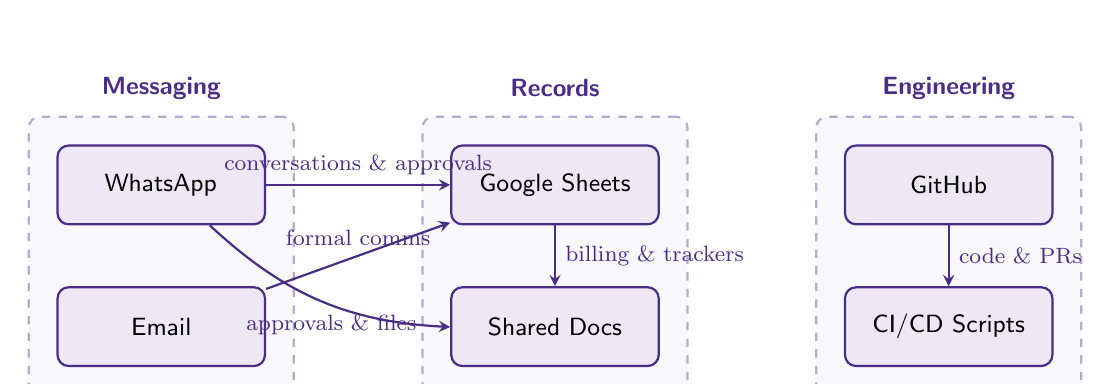
\begin{tikzpicture}[
    every node/.style={font=\sffamily\small},
    grouplabel/.style={font=\sffamily\bfseries\small, color=primary},
    box/.style={
        rectangle,
        rounded corners,
        draw=primary,
        fill=secondary,
        thick,
        text width=2.4cm,
        align=center,
        minimum height=1.0cm
    },
    grpbox/.style={draw=primary!40, dashed, thick, rounded corners, fill=primary!4, inner sep=10pt},
    arrow/.style={->, >=stealth, thick, color=primary}
]

% NODES
\node[box] (wa)    at (0, 1.6)  {WhatsApp};
\node[box] (email) at (0, -0.2) {Email};

\node[box] (sheets) at (5, 1.6)  {Google Sheets};
\node[box] (docs)   at (5, -0.2) {Shared Docs};

\node[box] (gh) at (10, 1.6)  {GitHub};
\node[box] (ci) at (10, -0.2) {CI/CD Scripts};

% GROUP BOXES
\begin{pgfonlayer}{background}
    \node[grpbox, fit=(wa)(email)] (msg) {};
    \node[grpbox, fit=(sheets)(docs)] (rec) {};
    \node[grpbox, fit=(gh)(ci)] (eng) {};
\end{pgfonlayer}

\node[grouplabel] at (msg.north) [yshift=0.35cm] {Messaging};
\node[grouplabel] at (rec.north) [yshift=0.35cm] {Records};
\node[grouplabel] at (eng.north) [yshift=0.35cm] {Engineering};

% ARROWS
\draw[arrow] (wa)    -- node[above, font=\footnotesize] {conversations \& approvals} (sheets);
\draw[arrow] (wa)    edge[bend right=20] node[below, font=\footnotesize, pos=0.55] {approvals \& files} (docs);
\draw[arrow] (gh)    -- node[right, font=\footnotesize] {code \& PRs} (ci);
\draw[arrow] (sheets) -- node[right, font=\footnotesize] {billing \& trackers} (docs);
\draw[arrow] (email) -- node[above, font=\footnotesize, pos=0.5] {formal comms} (sheets);

\end{tikzpicture}
}
\caption{Principal Tools and Dominant Information Flows in the Current System}
\end{figure}

\subsection{Tool-Based Operational Environment}
Because no single platform coordinates the company's work, each tool feeds into day-to-day operations independently. The hub-and-spoke view below illustrates how operations sit at the centre of several disconnected tools, with no direct integration between the spokes themselves.

\begin{figure}[H]
\centering
\resizebox{0.85\textwidth}{!}{
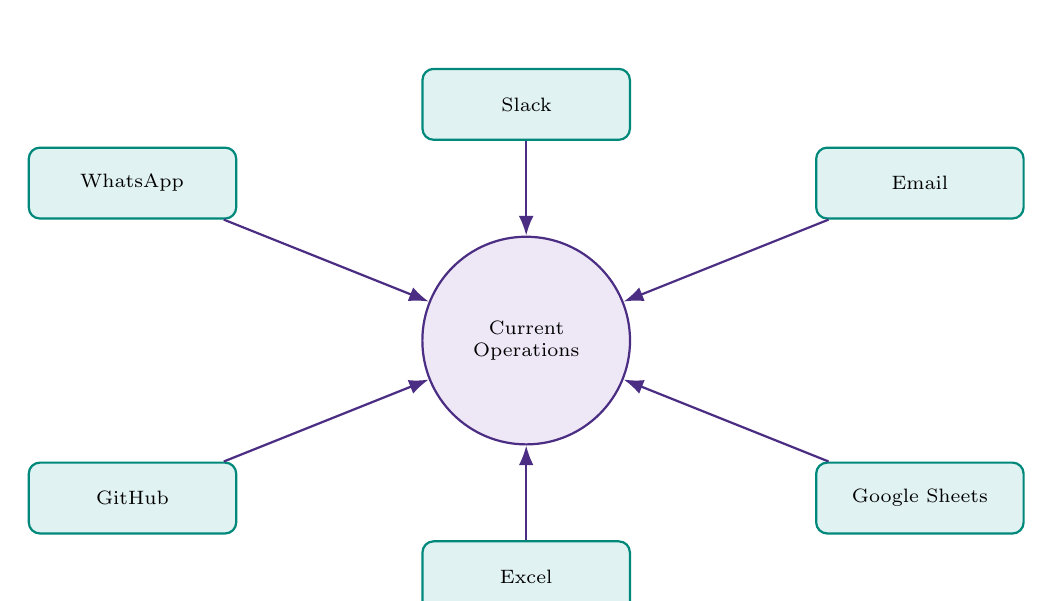
\begin{tikzpicture}[
    every node/.style={font=\scriptsize},
    tool/.style={
        rectangle,
        rounded corners,
        draw=accent,
        fill=softteal,
        thick,
        text width=2.4cm,
        minimum height=0.9cm,
        align=center
    },
    center/.style={
        circle,
        draw=primary,
        fill=secondary,
        thick,
        text width=2.3cm,
        minimum size=2.4cm,
        align=center
    },
    arrow/.style={thick, -{Latex[length=2.5mm]}, color=primary}
]

\node[center] (ops) at (0,0) {Current\\Operations};

\node[tool] (wa) at (-5,2) {WhatsApp};
\node[tool] (slack) at (0,3) {Slack};
\node[tool] (email) at (5,2) {Email};
\node[tool] (github) at (-5,-2) {GitHub};
\node[tool] (excel) at (0,-3) {Excel};
\node[tool] (sheets) at (5,-2) {Google Sheets};

\draw[arrow] (wa) -- (ops);
\draw[arrow] (slack) -- (ops);
\draw[arrow] (email) -- (ops);
\draw[arrow] (github) -- (ops);
\draw[arrow] (excel) -- (ops);
\draw[arrow] (sheets) -- (ops);

\end{tikzpicture}
}
\caption{Current Tool-Based Operational Environment}
\end{figure}

\section{Current Workflow}
The following sequence describes a typical workflow for handling a client request in the present environment:

\begin{enumerate}[leftmargin=2em]
    \item The client submits a request or approval via WhatsApp or email.
    \item The project manager (PM) or account lead records the request informally in chat and sometimes copies the details into a Google Sheet for tracking.
    \item The PM clarifies scope in chat and allocates work by creating tasks in GitHub or assigning developers directly.
    \item Developers implement the change and create pull requests; notifications are sent through chat channels.
    \item Quality assurance or the PM approves the change (often communicated via chat); deployment is executed with project-specific scripts.
    \item Financial and status updates are recorded manually in Sheets for billing and reporting.
\end{enumerate}

This workflow is practical for a small team and allows quick communication. However, it becomes less effective as the number of projects, clients, and developers increases. Since the workflow depends on manual coordination, project information can become scattered. For example, the client's requirement may be in WhatsApp, task progress may be in GitHub, and final reporting may be in Google Sheets. Without a centralised system, it becomes difficult to maintain a single source of truth.

\subsection{Current Workflow Diagram}

\begin{figure}[H]
\centering
\resizebox{0.85\textwidth}{!}{
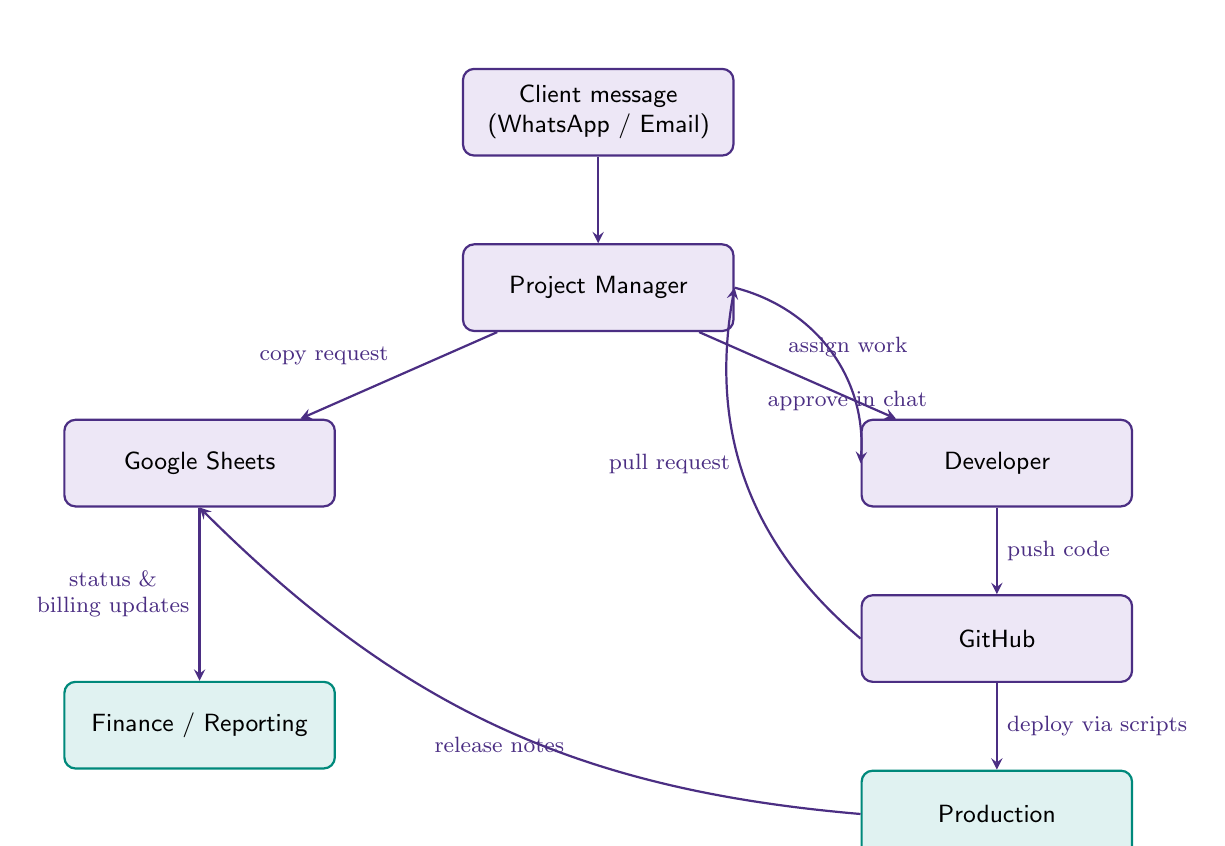
\begin{tikzpicture}[
    every node/.style={font=\sffamily\small},
    node distance=1.1cm and 1.6cm,
    box/.style={
        rectangle,
        rounded corners,
        draw=primary,
        fill=secondary,
        thick,
        text width=3.2cm,
        align=center,
        minimum height=1.1cm
    },
    extbox/.style={
        rectangle,
        rounded corners,
        draw=accent,
        fill=softteal,
        thick,
        text width=3.2cm,
        align=center,
        minimum height=1.1cm
    },
    arrow/.style={->, >=stealth, thick, color=primary}
]

\node[box] (client) {Client message\\(WhatsApp / Email)};
\node[box, below=of client] (pm) {Project Manager};
\node[box, below left=of pm] (sheets) {Google Sheets};
\node[box, below right=of pm] (dev) {Developer};
\node[box, below=of dev] (gh) {GitHub};
\node[extbox, below=of gh] (prod) {Production};
\node[extbox, below=2.2cm of sheets] (finance) {Finance / Reporting};

% ARROWS
\draw[arrow] (client) -- (pm);
\draw[arrow] (pm) -- node[above left, font=\footnotesize] {copy request} (sheets);
\draw[arrow] (pm) -- node[above right, font=\footnotesize, pos=0.4] {assign work} (dev);
\draw[arrow] (dev) -- node[right, font=\footnotesize] {push code} (gh);
\draw[arrow] (gh.west) to[bend left=30] node[left, font=\footnotesize, pos=0.55] {pull request} (pm.east);
\draw[arrow] (pm.east) to[bend left=40] node[below, font=\footnotesize, pos=0.65] {approve in chat} (dev.west);
\draw[arrow] (gh) -- node[right, font=\footnotesize] {deploy via scripts} (prod);
\draw[arrow] (sheets) -- node[left, font=\footnotesize, align=center] {status \&\\billing updates} (finance);
\draw[arrow] (prod.west) to[bend left=20] node[below, font=\footnotesize] {release notes} (sheets.south);

\end{tikzpicture}
}
\caption{Current Workflow for Handling a Client Request}
\end{figure}

\subsection{Operational Swimlane View}
To make the dependencies explicit, the swimlane diagram below maps the same workflow across three actors --- the client, the project manager, and the developer team. The shaded region highlights the high-dependency zone in which the project manager mediates almost every hand-off, and where information is exchanged through unstructured, informal channels.

\begin{figure}[H]
\centering
\resizebox{\textwidth}{!}{
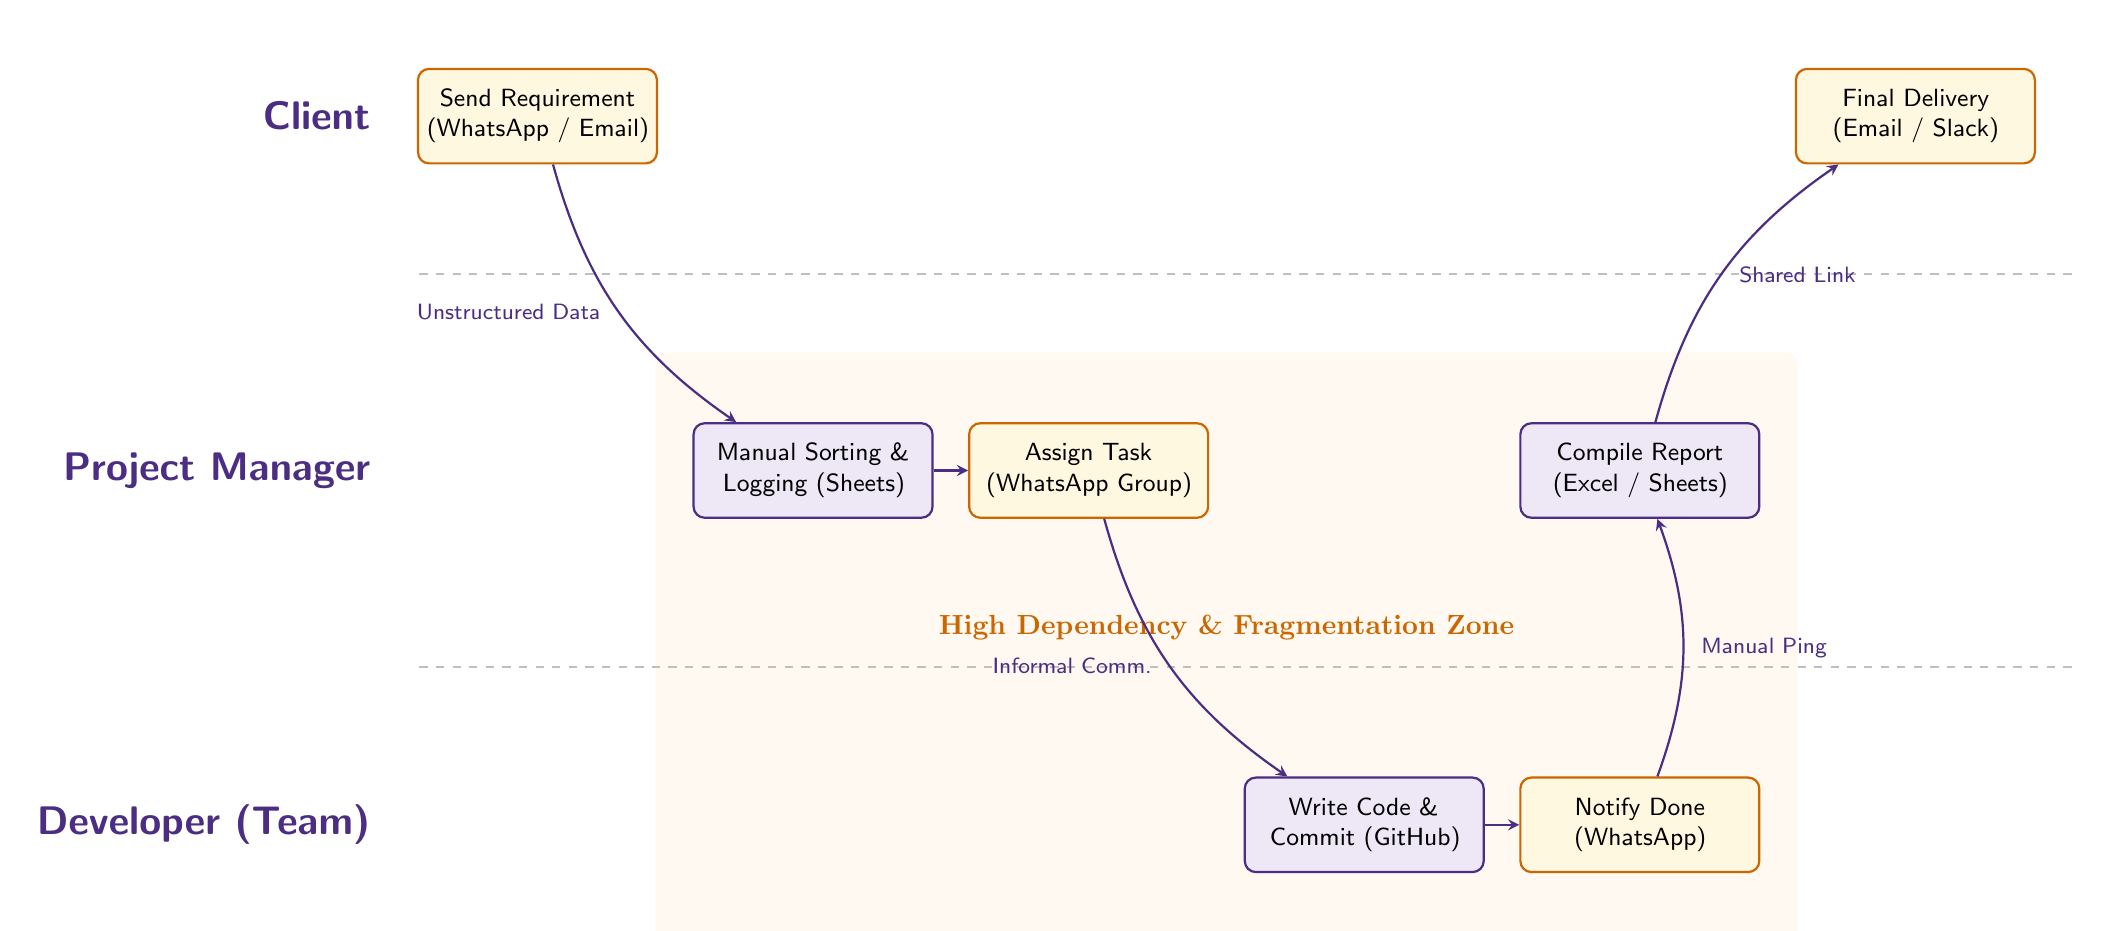
\begin{tikzpicture}[
    every node/.style={font=\sffamily\small},
    swimlane/.style={draw=gray!50, dashed, thick},
    box/.style={
        rectangle,
        rounded corners,
        draw=primary,
        fill=secondary,
        thick,
        text width=2.8cm,
        align=center,
        minimum height=1.2cm
    },
    riskbox/.style={
        rectangle,
        rounded corners,
        draw=orange!80!black,
        fill=softcream,
        thick,
        text width=2.8cm,
        align=center,
        minimum height=1.2cm
    },
    arrow/.style={->, >=stealth, thick, color=primary},
    labelnode/.style={font=\sffamily\Large\bfseries, color=primary}
]

% SWIMLANES
\draw[swimlane] (0,2.5) -- (21,2.5);
\draw[swimlane] (0,-2.5) -- (21,-2.5);

% LANE LABELS
\node[labelnode, left] at (-0.5, 4.5) {Client};
\node[labelnode, left] at (-0.5, 0) {Project Manager};
\node[labelnode, left] at (-0.5, -4.5) {Developer (Team)};

% NODES
\node[riskbox] (req) at (1.5, 4.5) {Send Requirement\\(WhatsApp / Email)};
\node[box] (log) at (5.0, 0) {Manual Sorting \&\\Logging (Sheets)};
\node[riskbox] (assign) at (8.5, 0) {Assign Task\\(WhatsApp Group)};
\node[box] (code) at (12.0, -4.5) {Write Code \&\\Commit (GitHub)};
\node[riskbox] (notify) at (15.5, -4.5) {Notify Done\\(WhatsApp)};
\node[box] (report) at (15.5, 0) {Compile Report\\(Excel / Sheets)};
\node[riskbox] (delivery) at (19.0, 4.5) {Final Delivery\\(Email / Slack)};

% ARROWS
\draw[arrow] (req) edge[bend right=20] node[left, xshift=-0.1cm] {\footnotesize Unstructured Data} (log);
\draw[arrow] (log) -- (assign);
\draw[arrow] (assign) edge[bend right=20] node[left, xshift=-0.1cm] {\footnotesize Informal Comm.} (code);
\draw[arrow] (code) -- (notify);
\draw[arrow] (notify) edge[bend right=20] node[right, xshift=0.1cm] {\footnotesize Manual Ping} (report);
\draw[arrow] (report) edge[bend left=20] node[right, xshift=0.1cm] {\footnotesize Shared Link} (delivery);

% BACKGROUND HIGHLIGHT FOR RISK AREA
\begin{pgfonlayer}{background}
    \fill[orange!5, rounded corners] (3.0, 1.5) rectangle (17.5, -6);
    \node[orange!80!black, font=\bfseries] at (10.25, -2.00) {High Dependency \& Fragmentation Zone};
\end{pgfonlayer}

\end{tikzpicture}
}
\caption{Current Operational Swimlane Diagram Showing the PM Bottleneck}
\end{figure}

\subsection{Process Interpretation}
The diagrams show that the present workflow is heavily dependent on the project manager as an intermediary between the client, the development team and the administrative record-keeping process. Information begins in chat or email, is then copied manually into Sheets, passed verbally or informally to developers, and finally reconciled again for finance and reporting. This arrangement provides flexibility, but it also introduces delays, duplication and a high risk of inconsistency because the same request is represented in several disconnected places.

\begin{highlightBox}
\textbf{System Observation:} The existing workflow works, but it is heavily dependent on manual communication. The system lacks a centralised dashboard where requirements, tasks, development progress, reports, and decisions can be tracked together.
\end{highlightBox}

\subsection*{Observations}
\begin{itemize}[leftmargin=2em]
    \item Decisions and approvals are frequently recorded only in informal chat channels and not attached to formal project artifacts.
    \item Multiple manual hand-offs and unstructured transfers of information increase the probability of errors and omissions.
    \item Financial and management reporting depend on manual reconciliation across disparate artefacts.
\end{itemize}

\section{Need for System Improvement}
The main need for improvement comes from the gap between the company's growing operational requirements and its current semi-structured information system. As NextStepBD handles more clients and more development tasks, the existing tool-based workflow becomes difficult to manage. Manual coordination can slow down decision-making, increase dependency on managers, and create confusion among developers. The current configuration of tools and processes generates several operational risks:

\begin{itemize}[leftmargin=2em]
    \item \textbf{Loss of authoritative approvals:} informal confirmations in chat are not reliably recorded against tasks.
    \item \textbf{Data inconsistency:} the absence of a canonical data store leads to duplication and conflicting records.
    \item \textbf{Manual process burden:} project managers and administrators devote substantial time to reconciliation and coordination rather than value-adding work.
    \item \textbf{Security and compliance exposure:} sensitive data is sometimes shared through insecure channels without audit trails.
    \item \textbf{Scalability limitations:} reliance on manual processes and key individuals creates bottlenecks that constrain growth.
\end{itemize}

A modern information system should not only store data but also connect people, processes, and tools. For NextStepBD, this means the improved system should connect client requirements, task assignment, developer work, communication history, reporting data, and project status. An appropriate improvement strategy must be pragmatic: it should preserve users' existing preferred communication channels while capturing and formalising the items that must be auditable and actionable.

\section{Problem Identification}
Through observation of the company's operations, informal interviews with team members, and an analysis of the current workflow, five priority problems have been identified that will be addressed in the remainder of this report. Each problem is presented with a concise description, an illustrative example and the principal stakeholders affected.

Before detailing the problems, it is useful to identify the stakeholders whose work is shaped by the current system. The table below summarises each stakeholder group, their primary concern, and the way the existing environment falls short for them. These groups are revisited throughout the report --- in the feasibility analysis, the planning chapter, and the interviews and questionnaires of Chapter~4.

\begin{table}[H]
\centering
\renewcommand{\arraystretch}{1.35}
\small
\begin{tabularx}{\textwidth}{|p{3cm}|X|X|}
\hline
\rowcolor{secondary}
\textbf{Stakeholder} & \textbf{Primary Concern} & \textbf{Current Pain Point} \\
\hline
Management (CEO) & Predictable delivery, profitability, and visibility into risk. & Limited real-time visibility; decisions rely on manually assembled, sometimes conflicting reports. \\
\hline
Project Managers & Coordinating clients and developers; protecting scope and billing. & Act as a single communication bridge and become a bottleneck; spend heavily on manual reconciliation. \\
\hline
Developers & Clear tasks, stable requirements, and minimal context switching. & Ambiguous, chat-based requirements and frequent tool switching reduce focus and cause rework. \\
\hline
QA / Team Leads & Releasing stable, reviewed code. & Ad-hoc testing and manual, chat-approved deployments increase the risk of defects reaching clients. \\
\hline
Finance / Operations & Accurate billing and reliable records. & Invoices depend on manual cross-referencing of disparate sheets, producing discrepancies. \\
\hline
HR & Smooth onboarding and reduced key-person dependency. & No skills inventory or documented handoffs; onboarding is slow and knowledge is concentrated in individuals. \\
\hline
Clients & Clear communication and traceable approvals. & Approvals are informal and hard to retrieve, creating uncertainty during billing or scope disputes. \\
\hline
\end{tabularx}
\caption{Stakeholder Analysis --- Concerns and Current Pain Points}
\end{table}

\subsection{Problem 1 --- Fragmented Communication and Collaboration}
\begin{problemBox}
Project decisions, approvals and important clarifications are routinely exchanged via informal messaging channels (e.g., WhatsApp) and are not consistently captured in structured project artefacts.
\end{problemBox}

The root of this problem is that NextStepBD treats conversational tools as both the communication channel \emph{and} the system of record. A message in a WhatsApp thread may contain a binding approval, a scope change, or a clarification that materially affects delivery, yet it is never promoted into a tracked, attributable artefact. Because these channels are unstructured and ephemeral, the same decision is interpreted differently by different team members, and there is no reliable way to reconstruct \emph{who} agreed to \emph{what}, and \emph{when}. As project volume grows, the cognitive burden of monitoring multiple chat threads compounds, and important items are silently lost between conversations.

\textbf{Illustrative example:} A client posts a one-line approval in a WhatsApp group; developers proceed without the PM adding the approval to the tracked requirement, later resulting in scope disagreement when the client claims a different feature was agreed.

\textbf{Impact:} Rework, missed approvals, client dissatisfaction, weakened billing evidence, and potential contractual disputes.

\textbf{Stakeholders:} Project management, development teams, QA, and clients.

\subsection{Problem 2 --- System Fragmentation and Lack of Integration}
\begin{problemBox}
Multiple independent tools are used without an integration strategy, requiring manual cross-referencing and reconciliation.
\end{problemBox}

Each tool in the current environment was adopted to solve a single local need --- GitHub for code, Sheets for tracking, WhatsApp for talking, email for formal correspondence --- but none of them share data. The result is a set of disconnected ``islands of information'' that must be bridged manually by staff acting as human integrations. Every time a fact changes in one place (a task status, a client contact, a billing figure), someone must remember to update it everywhere else, and in practice this rarely happens consistently. This absence of an integration layer is the structural cause from which several of the other problems descend: without connected systems there can be no single source of truth, no automated traceability, and no reliable cross-tool reporting.

\textbf{Illustrative example:} Customer and billing status are recorded in separate Google Sheets maintained by different teams, so an invoice is generated against an out-of-date feature list, leading to inconsistent invoicing and a reconciliation cycle.

\textbf{Impact:} High administrative overhead, duplicated effort, data drift between tools, and impaired decision quality from conflicting records.

\textbf{Stakeholders:} Operations, finance, project management, and executive management.

\subsection{Problem 3 --- Data Management and Governance Deficiencies}
\begin{problemBox}
There is no single source of truth for core business entities; data duplication and unsystematic updates compromise reporting and analysis.
\end{problemBox}

Core business entities --- customers, projects, requirements, and invoices --- have no canonical home and no defined owner. The same entity is re-created in several spreadsheets, each maintained by a different person with a different naming convention, and there is no validation, versioning, or audit trail to indicate which copy is authoritative. Without governance rules (mandatory fields, unique identifiers, retention policy, and clear stewardship), the organisation cannot trust its own data: reports must be assembled by hand from inconsistent sources, and every figure is open to dispute. This deficiency directly undermines billing accuracy and the leadership's ability to make data-driven decisions.

\textbf{Illustrative example:} Conflicting invoice records for the same client appear in two different trackers, producing an accounting discrepancy that takes several staff-hours to investigate and resolve.

\textbf{Impact:} Financial risk, billing errors, audit difficulty, and reduced managerial visibility into the true state of the business.

\textbf{Stakeholders:} Finance, executive management, and project management.

\subsection{Problem 4 --- Security and Access Control Risks}
\begin{problemBox}
Sensitive information is exchanged through informal channels without consistent access controls or audit trails.
\end{problemBox}

Because there is no central system, sensitive material --- client credentials, personally identifiable information (PII), and contractual details --- circulates through the same informal channels used for casual conversation. Access is governed by whoever happens to be in a chat group rather than by role, there is no logging of who viewed or changed sensitive data, and no defined retention or redaction policy. This creates exposure on two fronts: an external breach risk if a personal device or account is compromised, and an internal governance risk because the company cannot demonstrate, for audit or compliance purposes, who had access to what. As the client base spans multiple jurisdictions, this gap also carries contractual and regulatory weight.

\textbf{Illustrative example:} Credentials or PII are pasted into a WhatsApp transcript that persists indefinitely on multiple personal phones, with no record of access, no expiry, and no way to revoke it.

\textbf{Impact:} Risk of data breaches, regulatory non-compliance, loss of client trust, and reputational harm.

\textbf{Stakeholders:} Clients, legal/compliance, IT/security, and management.

\subsection{Problem 5 --- Scalability and Operational Bottlenecks}
\begin{problemBox}
Manual task assignment and single-point decision-making create performance constraints and dependency on individual staff.
\end{problemBox}

The current way of working scales linearly with headcount rather than with capability: every additional client or project adds proportional manual coordination, and that coordination is concentrated in a few key individuals --- chiefly the project managers --- who act as the routing layer for almost all work. This produces classic single-point-of-failure behaviour. When a key person is overloaded, on leave, or leaves the company, their undocumented knowledge and in-flight decisions leave with them, and the pipeline stalls. The lack of templates, role-based assignment, and onboarding structure means new hires take weeks to become productive, further limiting the organisation's ability to grow without a disproportionate rise in overhead.

\textbf{Illustrative example:} When the PM is unavailable for a day, routine approvals and task routing stall across several projects because no one else has the context or authority to proceed.

\textbf{Impact:} Reduced throughput, longer lead times, key-person risk, slow onboarding, and staff burnout.

\textbf{Stakeholders:} Human resources, team leads, project management, and developers.

\section{Problem Severity Overview}
The following graph shows the estimated severity level of the identified problems based on their impact on operations, stability, and scalability. The scores reflect both the frequency with which each problem disrupts delivery and the difficulty of recovering from its consequences.

\begin{figure}[H]
\centering
\resizebox{\textwidth}{!}{
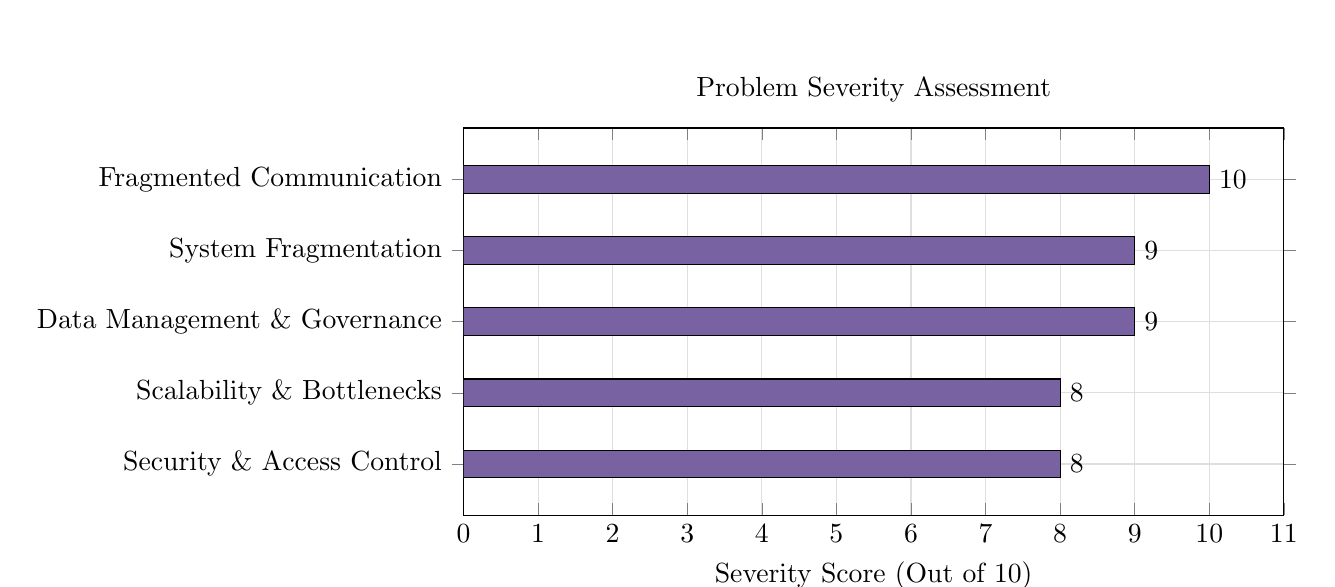
\begin{tikzpicture}
\begin{axis}[
    xbar,
    width=12cm,
    height=6.5cm,
    enlarge y limits=0.18,
    xmin=0,
    xmax=11,
    xlabel={Severity Score (Out of 10)},
    symbolic y coords={
        {Security \& Access Control},
        {Scalability \& Bottlenecks},
        {Data Management \& Governance},
        {System Fragmentation},
        {Fragmented Communication}
    },
    ytick=data,
    nodes near coords,
    grid=major,
    major grid style={draw=gray!25},
    title={Problem Severity Assessment}
]
\addplot[fill=primary!75] coordinates {
    (8,{Security \& Access Control})
    (8,{Scalability \& Bottlenecks})
    (9,{Data Management \& Governance})
    (9,{System Fragmentation})
    (10,{Fragmented Communication})
};
\end{axis}
\end{tikzpicture}
}
\caption{Estimated Severity of Identified Problems}
\end{figure}

\section{Summary of Identified Needs}
The analysis in this chapter suggests a set of core needs for the organisation:

\begin{enumerate}[leftmargin=2em]
    \item Mechanisms to capture and record authoritative approvals and decisions from informal channels.
    \item A canonical data store for customers, projects and requirements to reduce duplication and enable reliable reporting.
    \item Integration between collaboration tools and the canonical store to maintain familiar user interfaces while ensuring data integrity.
    \item Basic governance controls (RBAC, audit logs, PII handling) to reduce exposure.
    \item Automation of routine workflow tasks to reduce manual coordination and improve scalability.
\end{enumerate}

\section{Conclusion}
This chapter has established the organisational context and a set of well-defined problems that motivate the proposed system interventions. NextStepBD has successfully established a functional working system using available digital tools; however, the system lacks the structure, integration, and centralised control required for sustainable growth.

These problems compound one another: weak communication and data governance create task confusion, the lack of an integrated system enforces the project-manager bottleneck, and informal handling of sensitive data introduces security exposure. Therefore, the company needs an integrated information system that connects requirement management, task tracking, development workflow, communication history, and reliable reporting. The subsequent chapters will analyse requirements, evaluate feasibility, and propose concrete, phased solutions designed to be both practical and technically feasible within the organisation's operational constraints.

% ================================================================
% END OF CHAPTER 1
% ================================================================


% ================================================================
% START OF CHAPTER 2 — Initial Feasibility Study
% ================================================================
\chapter{Initial Feasibility Study}

\section{Introduction}
This chapter performs an initial feasibility study for the proposed improvement initiative at NextStepBD. The purpose of the study is to assess whether the recommended solution approach is technically possible, financially reasonable, operationally acceptable and realistic to implement within the organisation's time and resource constraints.

The proposed direction is not to replace the company's existing communication habits, but to support them with a structured and integrated information environment. Accordingly, the analysis considers five identified problems and sketches \textbf{three candidate solution strategies} that the organisation could adopt to address them. Each strategy is described in Chapter~4 against the same five problems, where a comparative Technical, Economic, Operational, and Schedule evaluation selects the recommended approach. The feasibility framework used in this chapter follows the standard \textbf{Technical, Economic, and Operational (TEO)} model, extended with a schedule dimension, and is applied per problem rather than per system so that the foundational feasibility of addressing each problem is established independently.

\begin{noteBox}
\textbf{Feasibility Focus:} The objective of this chapter is not only to propose solutions, but also to determine which solutions are realistic, affordable, and suitable for NextStepBD's current operational environment.
\end{noteBox}

\begin{table}[H]
\centering
\renewcommand{\arraystretch}{1.3}
\begin{tabularx}{\textwidth}{|p{4cm}|X|}
\hline
\rowcolor{secondary}
\textbf{Feasibility Dimension} & \textbf{Evaluation Question} \\
\hline
\textbf{Technical Feasibility} & Can the proposed solution be implemented using available technology, tools, infrastructure, and technical skills? \\
\hline
\textbf{Economic Feasibility} & Are the expected benefits greater than the cost of implementation, training, operation, and maintenance? \\
\hline
\textbf{Operational Feasibility} & Can the organisation realistically adopt and continue using the solution within its existing workflow and culture? \\
\hline
\textbf{Schedule Feasibility} & Can the solution be delivered incrementally within a realistic timeframe without disrupting billable work? \\
\hline
\end{tabularx}
\caption{TEO Feasibility Evaluation Criteria}
\end{table}

\begin{figure}[H]
\centering
\resizebox{\textwidth}{!}{
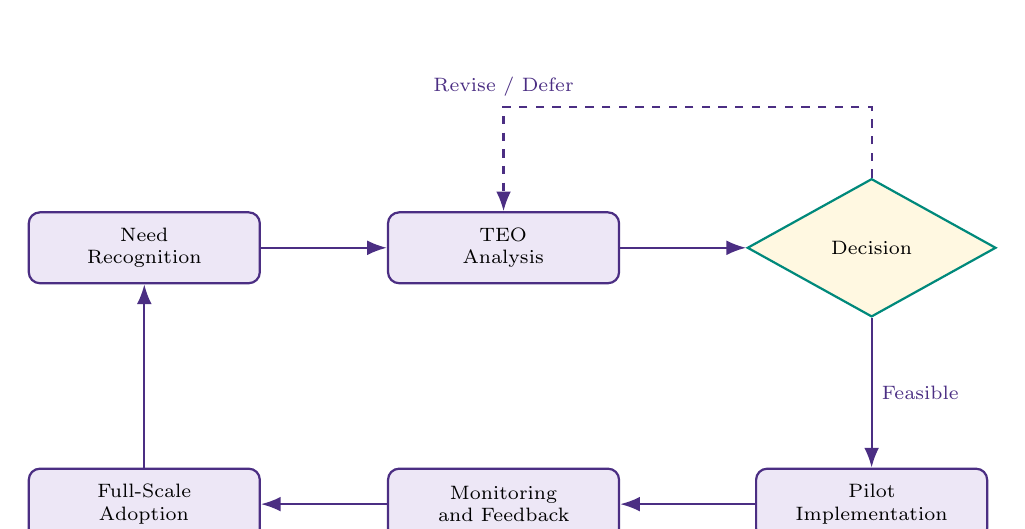
\begin{tikzpicture}[
    node distance=1.6cm,
    every node/.style={font=\scriptsize},
    process/.style={
        rectangle,
        rounded corners,
        draw=primary,
        fill=secondary,
        thick,
        text width=2.7cm,
        minimum height=0.9cm,
        align=center
    },
    decision/.style={
        diamond,
        draw=accent,
        fill=softcream,
        thick,
        aspect=1.8,
        text width=2.2cm,
        align=center
    },
    arrow/.style={thick, -{Latex[length=2.5mm]}, color=primary}
]

\node[process] (need) {Need\\Recognition};
\node[process, right=of need] (analysis) {TEO\\Analysis};
\node[decision, right=of analysis] (decision) {Decision};
\node[process, below=1.9cm of decision] (pilot) {Pilot\\Implementation};
\node[process] (monitor) at (analysis |- pilot) {Monitoring\\and Feedback};
\node[process] (scale) at (need |- pilot) {Full-Scale\\Adoption};

\draw[arrow] (need) -- (analysis);
\draw[arrow] (analysis) -- (decision);
\draw[arrow] (decision) -- node[right, font=\scriptsize]{Feasible} (pilot);
\draw[arrow] (pilot) -- (monitor);
\draw[arrow] (monitor) -- (scale);
\draw[arrow] (scale) -- (need);
\draw[arrow, dashed] (decision.north) -- ++(0,0.9) -| node[above, font=\scriptsize]{Revise / Defer} (analysis.north);

\end{tikzpicture}
}
\caption{Initial Feasibility Governance Cycle for NextStepBD}
\end{figure}

\section{Initial Feasibility Analysis}

\textbf{Baseline Assumptions for Calculations:} NextStepBD is defined as an organisation of approximately 50 employees (developers, UI/UX, QA, PMs). Economic feasibility assumes an internal exchange mapping of \$1 USD $\approx$ 120 BDT. All software cost estimations are based on standardised enterprise monthly licensing fees. Employee training costs assume an average internal valuation of \$15/hour per developer.

\subsection{Problem 01 --- Fragmented Communication and Collaboration}

\begin{problemBox}
Important decisions, approvals and clarifications are frequently communicated through informal channels such as WhatsApp and email. These exchanges are not consistently captured in a formal project record, which leads to misunderstandings, repeated clarification cycles and scope disputes.
\end{problemBox}

\textbf{Technical feasibility.} This problem is highly feasible to address because the company can keep using the communication tools it already uses while adding a capture layer to record important decisions. A central platform can receive message metadata, manual confirmations or webhook-triggered events and convert them into structured records. Since the initial solution does not require replacing WhatsApp or email, the technical effort is moderate and can be implemented incrementally.

\textbf{Economic feasibility.} The economic cost is reasonable because the organisation can begin with a small pilot and use a limited number of integrations. The company will not need to build a complete messaging platform from scratch. Instead, it can invest in lightweight automation, integration services and a collaboration tool subscription or configuration. The expected return comes from fewer missed approvals, less rework and fewer delays.

\textbf{Operational feasibility.} The proposed solution aligns well with current user behaviour because staff and clients can continue using familiar communication channels. Important items are simply captured into a formal system. This makes the solution operationally feasible and acceptable to users, provided that the capture process is simple and does not add unnecessary friction.

\textbf{Schedule feasibility.} This problem can be addressed early in the project because it depends mostly on workflow design, integration, and configuration of existing tools. A basic pilot can be delivered within a short timeframe, especially if the organisation starts with a small number of project teams.

\begin{table}[H]
\centering
\renewcommand{\arraystretch}{1.3}
\begin{tabularx}{\textwidth}{|p{3cm}|p{2.5cm}|X|}
\hline
\rowcolor{secondary}
\textbf{Dimension} & \textbf{Rating} & \textbf{Justification} \\
\hline
Technical & High & A capture layer can be built on top of existing tools using native webhooks and APIs; no replacement required. \\
\hline
Economic & High & Lightweight automation and a single collaboration subscription are offset by reduced rework and missed approvals. \\
\hline
Operational & High & Users keep familiar channels; only the formalisation step is new. \\
\hline
Overall Viability & Very Feasible & Recommended as an early, high-impact win. \\
\hline
\end{tabularx}
\caption{Communication Capture --- TEO Feasibility Summary}
\end{table}

\begin{summaryBox}
This problem is highly feasible to address because it can be improved without replacing the company's existing communication channels. The technical effort is moderate, the cost is manageable, and the operational impact is positive because users keep working in familiar tools while approvals are captured more reliably.
\end{summaryBox}

\begin{recommendBox}
\textbf{Priority Action:} Introduce a lightweight capture layer that records approvals and decisions from existing channels into a structured project record.

\textbf{Business Value:} Eliminates lost approvals and creates an auditable trail without disrupting how staff and clients already communicate.
\end{recommendBox}

\subsection{Problem 02 --- System Fragmentation and Lack of Integration}

\begin{problemBox}
The company currently uses several disconnected tools such as Google Sheets, GitHub, email and chat applications. Because these systems are not integrated, data must be copied manually and frequently becomes inconsistent.
\end{problemBox}

\textbf{Technical feasibility.} This problem is technically feasible to solve using a central data layer, APIs and connectors. Existing tools provide standard APIs and webhooks, which makes integration practical. A canonical database can act as the source of truth while other tools exchange data through controlled interfaces.

\textbf{Economic feasibility.} The cost of integration is moderate. It is cheaper to connect existing tools than to replace them. The main investment is in integration development, data mapping and maintenance. The long-term benefit is reduced duplication and lower administrative overhead.

\textbf{Operational feasibility.} A central integration approach is operationally appropriate because it reduces the need for staff to cross-check multiple records manually. However, it must be introduced carefully to avoid disrupting existing work habits. The integration should therefore be gradual and focused on high-value processes first.

\textbf{Schedule feasibility.} The problem can be solved in phases. The first phase can connect a small number of sources, such as Sheets and GitHub, before more complex sources are added. This phased approach is schedule-feasible and reduces implementation risk.

\begin{table}[H]
\centering
\renewcommand{\arraystretch}{1.3}
\begin{tabularx}{\textwidth}{|p{4cm}|X|X|}
\hline
\rowcolor{secondary}
\textbf{Area} & \textbf{Current State} & \textbf{Proposed State} \\
\hline
Data Location & Scattered across Sheets, GitHub, email & Canonical database as single source of truth \\
\hline
Synchronisation & Manual copy-paste between tools & Automated sync via APIs and webhooks \\
\hline
Consistency & Frequent duplication and conflicts & Controlled interfaces enforce one record \\
\hline
\end{tabularx}
\caption{System Integration --- Current vs Proposed State}
\end{table}

\begin{summaryBox}
This problem is highly feasible because it can be solved incrementally through standard integrations. The cost is reasonable, the implementation can be phased, and the operational benefit is strong because staff will no longer need to manually reconcile disconnected tools.
\end{summaryBox}

\begin{recommendBox}
\textbf{Priority Action:} Establish a canonical data layer and connect existing tools through phased API/webhook integrations.

\textbf{Business Value:} Removes isolated information silos and provides one reliable, automatically synchronised source for project data.
\end{recommendBox}

\subsection{Problem 03 --- Data Management and Governance Deficiencies}

\begin{problemBox}
No single authoritative data repository exists for customers, projects and requirements. As a result, duplicate records and conflicting updates occur, which weakens reporting and managerial control.
\end{problemBox}

\textbf{Technical feasibility.} A central database with carefully designed entities, validation rules and audit logging is technically straightforward for a software company to implement. Modern relational databases and integration frameworks are mature and reliable.

\textbf{Economic feasibility.} The cost is justified because poor data management directly affects billing accuracy, reporting and decision-making. Improving data quality reduces hidden costs such as manual reconciliation and rework. Although there is some upfront design and migration effort, the long-term savings are substantial.

\textbf{Operational feasibility.} This improvement is operationally feasible because it gives management a clearer view of business information. The main challenge is ensuring that users trust the central system and use it consistently. This can be addressed by making the system the preferred source for reporting and task linkage.

\textbf{Schedule feasibility.} This problem should be addressed early, but it does not need to be solved all at once. Core data entities can be introduced first, and existing records can be migrated gradually. This makes the schedule manageable.

\begin{table}[H]
\centering
\renewcommand{\arraystretch}{1.3}
\begin{tabularx}{\textwidth}{|p{3cm}|p{2.5cm}|X|}
\hline
\rowcolor{secondary}
\textbf{Dimension} & \textbf{Rating} & \textbf{Justification} \\
\hline
Technical & High & Relational databases, validation rules and audit logging are mature, well-understood technologies. \\
\hline
Economic & High & Better data quality directly improves billing accuracy and reduces costly reconciliation. \\
\hline
Operational & Med-High & Value is clear, but consistent adoption and trust in the central record must be cultivated. \\
\hline
Overall Viability & Feasible (phased) & Strategically important; introduce core entities first and migrate gradually. \\
\hline
\end{tabularx}
\caption{Data Governance --- TEO Feasibility Summary}
\end{table}

\begin{summaryBox}
This problem is feasible and strategically important. A central database and governance model are technically straightforward, economically justified, and operationally valuable because they improve reporting accuracy and reduce duplication.
\end{summaryBox}

\begin{recommendBox}
\textbf{Priority Action:} Define a canonical data model for customers, projects and requirements, with validation and audit logging, then migrate records in stages.

\textbf{Business Value:} Produces trustworthy reporting, eliminates conflicting records, and strengthens managerial visibility and billing accuracy.
\end{recommendBox}

\subsection{Problem 04 --- Security and Access Control Risks}

\begin{problemBox}
Sensitive information is sometimes shared through informal channels and there is no consistent access control or audit trail for data changes. This creates risk for the organisation and its clients.
\end{problemBox}

\textbf{Technical feasibility.} The problem is feasible to address through role-based access control, central authentication, audit logging and improved handling of sensitive fields. These are standard features in modern systems and can be built using existing identity management tools and secure storage practices.

\textbf{Economic feasibility.} The financial justification is strong because security incidents, data leaks and compliance failures can be costly. Implementing security controls is cheaper than dealing with the consequences of a breach. Much of the required capability can also be provided by open-source or managed services.

\textbf{Operational feasibility.} Security controls are operationally feasible, but they must be introduced in a way that does not obstruct daily work. Access rules should match actual roles, and approval workflows should remain simple. If controls are too strict or difficult to use, staff may try to bypass them.

\textbf{Schedule feasibility.} Basic security controls can be introduced alongside the early platform work. Authentication, role mapping and audit logging should be part of the first release rather than postponed, because security is a foundational requirement.

\begin{table}[H]
\centering
\renewcommand{\arraystretch}{1.3}
\begin{tabularx}{\textwidth}{|p{3cm}|p{2.5cm}|X|}
\hline
\rowcolor{secondary}
\textbf{Dimension} & \textbf{Rating} & \textbf{Justification} \\
\hline
Technical & High & RBAC, central authentication and audit logging are standard, available capabilities. \\
\hline
Economic & High & Controls are far cheaper than the cost of a breach or compliance failure. \\
\hline
Operational & Medium & Must be role-aware and lightweight, otherwise staff may bypass the controls. \\
\hline
Overall Viability & Necessary \& Feasible & Treat as a baseline requirement embedded in the first release. \\
\hline
\end{tabularx}
\caption{Security \& Access Control --- TEO Feasibility Summary}
\end{table}

\begin{summaryBox}
This problem is feasible and should be treated as a baseline requirement. The technical controls are standard and available, the cost is justified by risk reduction, and the operational fit is strong if the controls are designed to be lightweight and role-aware.
\end{summaryBox}

\begin{recommendBox}
\textbf{Priority Action:} Embed role-based access control, central authentication and audit logging into the foundational release.

\textbf{Business Value:} Protects client data and credentials, provides an audit trail, and reduces regulatory and reputational risk.
\end{recommendBox}

\subsection{Problem 05 --- Scalability and Operational Bottlenecks}

\begin{problemBox}
Manual processes, single-person dependencies and a lack of standardised workflow create bottlenecks as the team grows. The company becomes increasingly dependent on a few key individuals.
\end{problemBox}

\textbf{Technical feasibility.} This problem is technically feasible to solve through workflow automation, task templates, role-based assignment and monitoring. These are not highly experimental capabilities; they are common in process-oriented software environments.

\textbf{Economic feasibility.} The problem has strong economic justification because it directly affects productivity, speed of delivery and staff utilisation. Reducing bottlenecks improves throughput and helps the company handle more projects without a proportional increase in overhead.

\textbf{Operational feasibility.} The solution is operationally feasible if the company accepts more structured work assignment and task visibility. Existing staff can keep their familiar collaboration tools, while the structured system ensures that no work item depends on memory or personal follow-up alone.

\textbf{Schedule feasibility.} Scalability improvements should be introduced in parallel with workflow and integration improvements. They can begin with templates, notifications and assignment rules, then expand into richer automation as the organisation matures.

\begin{table}[H]
\centering
\renewcommand{\arraystretch}{1.3}
\begin{tabularx}{\textwidth}{|p{3cm}|p{2.5cm}|X|}
\hline
\rowcolor{secondary}
\textbf{Dimension} & \textbf{Rating} & \textbf{Justification} \\
\hline
Technical & High & Workflow automation, templates and role-based assignment are common, proven features. \\
\hline
Economic & High & Reducing bottlenecks raises throughput without a proportional rise in overhead. \\
\hline
Operational & High & Staff keep familiar tools; structure ensures no task depends on a single person's memory. \\
\hline
Overall Viability & Highly Feasible & Introduce in parallel with workflow and integration work. \\
\hline
\end{tabularx}
\caption{Scalability \& Workflow --- TEO Feasibility Summary}
\end{table}

\begin{summaryBox}
This problem is highly feasible because workflow automation and role-based assignment are common features in modern systems. The cost is moderate, the benefits are significant, and the changes fit the organisation's need to reduce dependence on a few key individuals.
\end{summaryBox}

\begin{recommendBox}
\textbf{Priority Action:} Introduce task templates, role-based assignment rules and monitoring to standardise work and remove single-person dependencies.

\textbf{Business Value:} Increases delivery throughput, improves staff utilisation, and lets the company scale without proportional management overhead.
\end{recommendBox}

\section{Comparative Feasibility Summary}
The table below summarises the relative feasibility of each problem area.

\begin{table}[H]
\centering
\renewcommand{\arraystretch}{1.4}
\small
\begin{tabularx}{\textwidth}{|>{\raggedright\arraybackslash}X|c|c|c|c|c|}
\hline
\rowcolor{secondary}
\textbf{Problem} & \textbf{Tech.} & \textbf{Econ.} & \textbf{Ops.} & \textbf{Sched.} & \textbf{Overall Assessment} \\
\hline
Fragmented Communication \& Collaboration & High & High & High & High & Very feasible \\
\hline
System Fragmentation \& Lack of Integration & High & High & Med-High & Med-High & Very feasible \\
\hline
Data Management \& Governance Deficiencies & High & High & Med-High & Medium & Feasible (phased migration) \\
\hline
Security \& Access Control Risks & High & High & Medium & High & Necessary and feasible \\
\hline
Scalability \& Operational Bottlenecks & High & High & High & Med-High & Highly feasible \\
\hline
\end{tabularx}
\caption{Comparative Feasibility Analysis of the Five Identified Problems}
\end{table}

\begin{figure}[H]
\centering
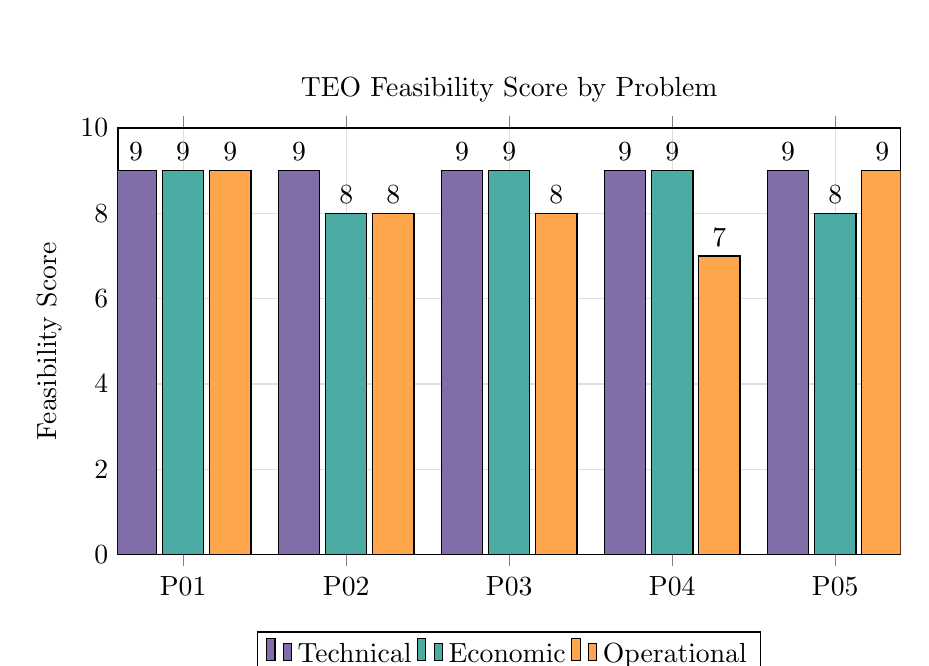
\begin{tikzpicture}
\begin{axis}[
    ybar,
    width=0.95\textwidth,
    height=7cm,
    bar width=15pt,
    ymin=0,
    ymax=10,
    ylabel={Feasibility Score},
    symbolic x coords={P01,P02,P03,P04,P05},
    xtick=data,
    nodes near coords,
    nodes near coords align={vertical},
    legend style={at={(0.5,-0.18)}, anchor=north, legend columns=3},
    grid=major,
    major grid style={draw=gray!25},
    title={TEO Feasibility Score by Problem}
]
\addplot[fill=primary!70] coordinates {(P01,9) (P02,9) (P03,9) (P04,9) (P05,9)};
\addplot[fill=accent!70] coordinates {(P01,9) (P02,8) (P03,9) (P04,9) (P05,8)};
\addplot[fill=orange!70] coordinates {(P01,9) (P02,8) (P03,8) (P04,7) (P05,9)};
\legend{Technical, Economic, Operational}
\end{axis}
\end{tikzpicture}
\caption{Technical, Economic, and Operational Feasibility Comparison}
\end{figure}

\textbf{Interpretation}
\begin{itemize}[leftmargin=2em]
    \item All five problems are feasible to address, but they should not be approached as separate, unrelated projects.
    \item A shared governed-data foundation is required by any of the realistic solution strategies; without it, downstream fixes to communication, fragmentation, or governance tend to reproduce the same inconsistency in new places.
    \item Process formalisation (requirements, approvals, task routing, escalation) and delivery automation (CI/CD, monitoring, incident response) are needed in addition to the foundation, and the right way to combine them is a strategic choice rather than a foregone conclusion.
    \item Security and access control must be designed as a shared service across whatever system is selected, not bolted on after the fact.
\end{itemize}

\section{Indicative Implementation Considerations}
Regardless of which solution strategy is ultimately selected, certain implementation principles apply to all of them. The detail of the chosen roadmap is developed in Chapter~4 (Section~4.4) once the strategy is fixed, and the full release plan, decision gates, and acceptance framework are elaborated in Chapter~5 (Design). This chapter therefore states the principles only, not the specific phase plan.

\begin{itemize}[leftmargin=2em]
    \item \textbf{Foundation before process, and process before delivery.} A governed data model, identity, audit, and integration core must be in place before workflow changes and delivery automation can be relied upon. Reversing this order produces tools that look integrated but still depend on manual reconciliation.
    \item \textbf{Incremental over big-bang.} Each release should be small enough to be measured, reversible, and isolated from billable work. The pilot should run on real projects, not on a synthetic dataset, and should exit cleanly if it does not meet its acceptance criteria.
    \item \textbf{Configuration over rebuild.} Where a mature commercial product (collaboration, monitoring, identity, observability) already meets the requirement, it should be configured rather than replaced by custom code, so that engineering effort is reserved for the unique integration and governance layer.
    \item \textbf{Remove the old record before adding the new one.} Each rollout phase should include a decision about which spreadsheet, manual report, or informal approval practice will be retired; otherwise the new system becomes additional work and never realises the saving.
    \item \textbf{Security is cross-cutting, not optional.} Role-based access, central authentication, audit logging, and redaction are introduced in the foundation release and enforced across every later layer.
    \item \textbf{Process ownership is named early.} Data, workflow, integration, and security owners are assigned before the pilot starts; without explicit ownership, validation rules, dashboards, and access lists gradually become unreliable.
\end{itemize}

\noindent The detailed release plan, twenty-four-week Gantt, decision gates, and pilot acceptance framework for the recommended strategy are developed in Chapter~4 and elaborated in Chapter~5.

\section{Implementation Priority}
While all five problems are feasible, they differ in urgency. The chart below ranks the proposed improvements by implementation priority, balancing the severity established in Chapter 1 against the dependency each item has on the shared foundation.

\begin{figure}[H]
\centering
\resizebox{\textwidth}{!}{
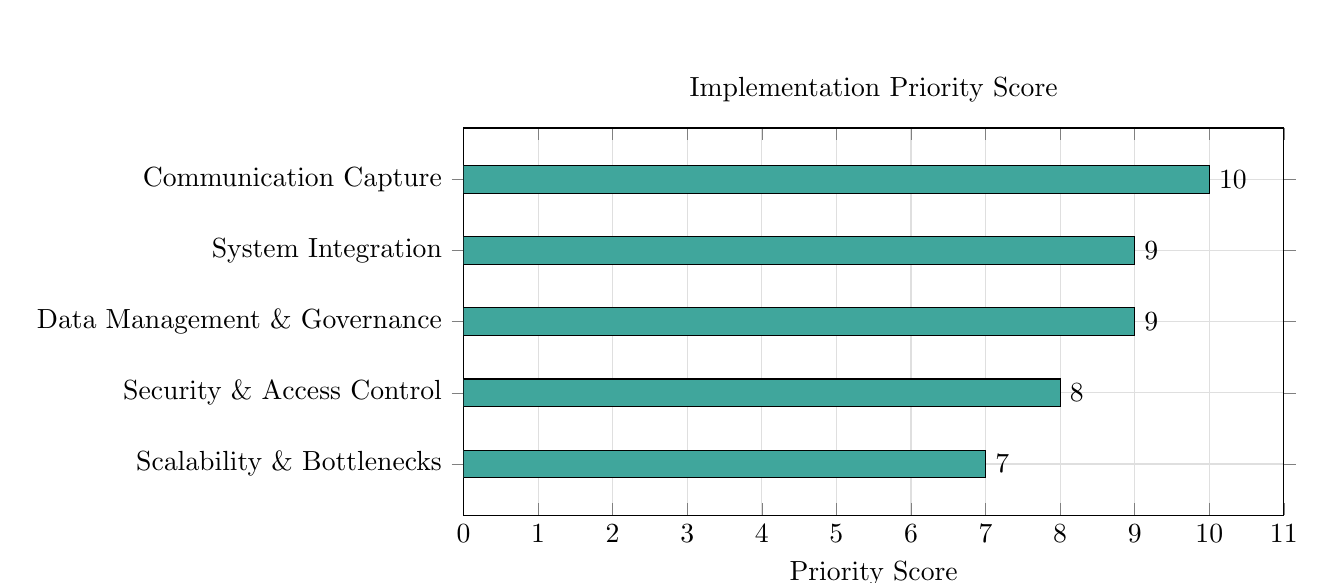
\begin{tikzpicture}
\begin{axis}[
    xbar,
    width=12cm,
    height=6.5cm,
    enlarge y limits=0.18,
    xmin=0,
    xmax=11,
    xlabel={Priority Score},
    symbolic y coords={
        {Scalability \& Bottlenecks},
        {Security \& Access Control},
        {Data Management \& Governance},
        {System Integration},
        {Communication Capture}
    },
    ytick=data,
    nodes near coords,
    grid=major,
    major grid style={draw=gray!25},
    title={Implementation Priority Score}
]
\addplot[fill=accent!75] coordinates {
    (7,{Scalability \& Bottlenecks})
    (8,{Security \& Access Control})
    (9,{Data Management \& Governance})
    (9,{System Integration})
    (10,{Communication Capture})
};
\end{axis}
\end{tikzpicture}
}
\caption{Priority Ranking of Proposed Improvements}
\end{figure}

\section{Conclusion}
The initial feasibility study shows that the proposed solution is realistic, implementable and economically justified. None of the five identified problems requires a fully custom end-to-end platform to be built at once. Instead, the recommended approach is to combine a central integration layer, a configured collaboration tool, and a DevOps/observability platform in a phased implementation.

The company does not need heavy capital injections; rather, it requires an overhaul of its organisational workflow and engineering principles. The most urgent changes are establishing reliable communication capture and a central integration layer, because every other improvement depends on that shared foundation. This approach balances technical feasibility, user acceptance and organisational capacity while addressing the core operational weaknesses identified in Chapter 1.

% ================================================================
% END OF CHAPTER 2
% ================================================================


% ================================================================
% START OF CHAPTER 3 — Project Planning
% ================================================================
\chapter{Project Planning}

\section{Introduction}
This chapter presents the project plan for NextStepBD's improvement initiative. It sets out the scope, schedule, stakeholder engagement approach, cost considerations and quality arrangements that will guide design and pilot activities. The chapter draws on the problem statements and feasibility analysis in Chapters 1 and 2 and translates those findings into a practical plan for review and approval.

The chapter uses standard project-planning terms. It covers scope refinement, schedule development, stakeholder engagement, cost considerations and quality planning. Because the organisation will keep its current communication channels, the plan focuses on integrating informal inputs safely and with minimal disruption. The emphasis is on preparation: analysis, stakeholder validation, pilot design and monitoring setup.

\begin{highlightBox}
\textbf{Planning Focus:} This chapter explains how the project plan is developed for each priority problem. For every problem it presents a Work Breakdown Structure (WBS), a planning-focused Gantt chart, a record of stakeholder validation, and high-level cost and quality plans --- all scoped to preparation and pilot activities rather than full rollout.
\end{highlightBox}

\section{Planning in NextStepBD}
Project governance for this initiative will be established as a lightweight, accountable structure appropriate for a small-to-medium software services company. The governance model comprises an executive sponsor (senior company partner), a project manager (internal PM/PO), a small steering committee (executive sponsor, head of delivery, head of operations, finance representative), and a cross-functional project team (backend developer, integration specialist, QA/DevOps engineer, business analyst). External consultants may be engaged for specialised integration tasks as required.

Scope definition will be constrained to planning and pilot preparation activities during the initial project phase; the intention is to deliver planning artefacts, validated designs and pilots that demonstrate the expected operational improvements before full organisational rollout. Baseline planning deliverables include Work Breakdown Structures (WBS) for each identified problem area, detailed schedules (Gantt), stakeholder engagement records and a draft cost and quality management plan. Risk management and procurement strategies will be described in follow-up documentation but are considered in the schedule and stakeholder planning herein.

\begin{figure}[H]
\centering
\resizebox{0.95\textwidth}{!}{
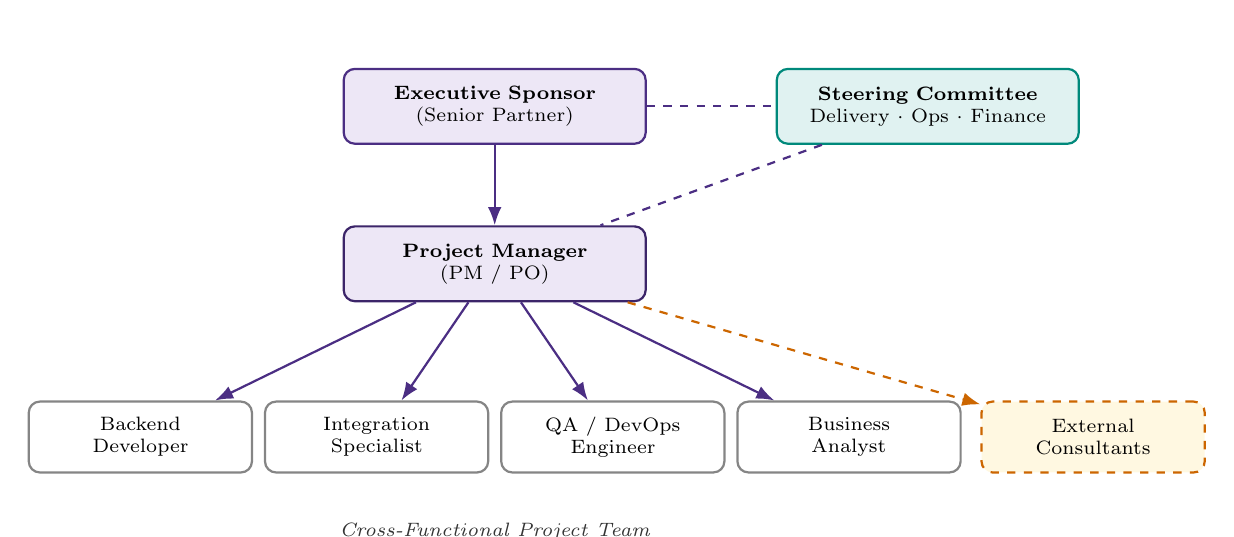
\begin{tikzpicture}[
    every node/.style={font=\scriptsize},
    sponsor/.style={rectangle, rounded corners, draw=primary, fill=secondary, thick, text width=3.6cm, minimum height=0.95cm, align=center},
    committee/.style={rectangle, rounded corners, draw=accent, fill=softteal, thick, text width=3.6cm, minimum height=0.95cm, align=center},
    pm/.style={rectangle, rounded corners, draw=primary!80!black, fill=secondary, thick, text width=3.6cm, minimum height=0.95cm, align=center},
    team/.style={rectangle, rounded corners, draw=darkgray!60, fill=white, thick, text width=2.6cm, minimum height=0.9cm, align=center},
    ext/.style={rectangle, rounded corners, draw=orange!80!black, fill=softcream, dashed, thick, text width=2.6cm, minimum height=0.9cm, align=center},
    arrow/.style={thick, -{Latex[length=2.3mm]}, color=primary},
    line/.style={thick, color=primary}
]

\node[sponsor] (sponsor) at (0,0) {\textbf{Executive Sponsor}\\(Senior Partner)};
\node[committee] (committee) at (5.5,0) {\textbf{Steering Committee}\\Delivery $\cdot$ Ops $\cdot$ Finance};
\node[pm] (pm) at (0,-2) {\textbf{Project Manager}\\(PM / PO)};

\draw[arrow] (sponsor) -- (pm);
\draw[line, dashed] (sponsor) -- (committee);
\draw[line, dashed] (committee) -- (pm);

% Team members
\node[team] (be)  at (-4.5,-4.2) {Backend\\Developer};
\node[team] (int) at (-1.5,-4.2) {Integration\\Specialist};
\node[team] (qa)  at (1.5,-4.2) {QA / DevOps\\Engineer};
\node[team] (ba)  at (4.5,-4.2) {Business\\Analyst};
\node[ext]  (ext) at (7.6,-4.2) {External\\Consultants};

\draw[arrow] (pm) -- (be);
\draw[arrow] (pm) -- (int);
\draw[arrow] (pm) -- (qa);
\draw[arrow] (pm) -- (ba);
\draw[arrow, color=orange!80!black, dashed] (pm) -- (ext);

\node[font=\scriptsize\itshape, color=darkgray] at (0,-5.4) {Cross-Functional Project Team};

\end{tikzpicture}
}
\caption{Project Governance Structure for the Planning Initiative}
\end{figure}

\section{Planning to Resolve the Problems}
This section presents planning activities tailored to each of the priority problems identified in Chapter 1. For each problem the chapter provides a Work Breakdown Structure (WBS); a Gantt chart derived from the WBS focusing on analysis and planning activities; a synthetic record of stakeholder validation and feedback; high-level cost management considerations; and a problem-specific quality management plan. The WBS and Gantt charts are deliberately planning-focused and do not assume implementation progress beyond preparation, pilot configuration and validation.

% ----------------------------------------------------------------
% PROBLEM 01
% ----------------------------------------------------------------
\subsection{Problem 01 --- Fragmented Communication \& Collaboration}

\textbf{Problem context.} NextStepBD depends heavily on chat-based communication for approvals, clarification, and day-to-day coordination. In practice, important decisions can remain buried in long message threads, which makes it difficult to trace what was agreed, who approved it, and which work item it relates to. This creates delays, repeated clarification, and weak evidence for delivery decisions.

\subsubsection{Schedule Management}
The Work Breakdown Structure (WBS) below decomposes the planning effort into nine work packages, from problem analysis through to documentation.

\begin{table}[H]
\centering
\renewcommand{\arraystretch}{1.25}
\small
\begin{tabularx}{\textwidth}{|c|p{4.2cm}|X|}
\hline
\rowcolor{secondary}
\textbf{WBS} & \textbf{Work Package} & \textbf{Key Activities} \\
\hline
1.1 & Problem Analysis & Review chat message patterns and sample threads; identify decision/approval artefacts and their distribution. \\
\hline
1.2 & Root Cause Validation & Verify communication dependency on PMs; map failed handoffs and typical consequences. \\
\hline
1.3 & Stakeholder Review & Facilitate validation workshop (PMs, developers, account managers); document inputs and acceptance criteria. \\
\hline
1.4 & Requirement Refinement & Define capture requirements (what is an ``official'' approval); specify operator review UI requirements. \\
\hline
1.5 & Solution Design & Design capture flow and API contract to central platform; define UX for one-click confirmation. \\
\hline
1.6 & Implementation Planning & Define pilot scope and success metrics; identify pilot teams and access requirements. \\
\hline
1.7 & Testing \& Validation Planning & Define test cases for capture accuracy and latency; plan pilot acceptance tests and measurement method. \\
\hline
1.8 & Monitoring \& Evaluation Planning & Define monitoring KPIs (capture rate, error rate); establish dashboard and reporting cadence. \\
\hline
1.9 & Documentation & Prepare user guides and operator runbook; prepare stakeholder sign-off package. \\
\hline
\end{tabularx}
\caption{WBS --- Problem 01: Fragmented Communication \& Collaboration}
\end{table}

\begin{figure}[H]
\centering
\resizebox{\textwidth}{!}{
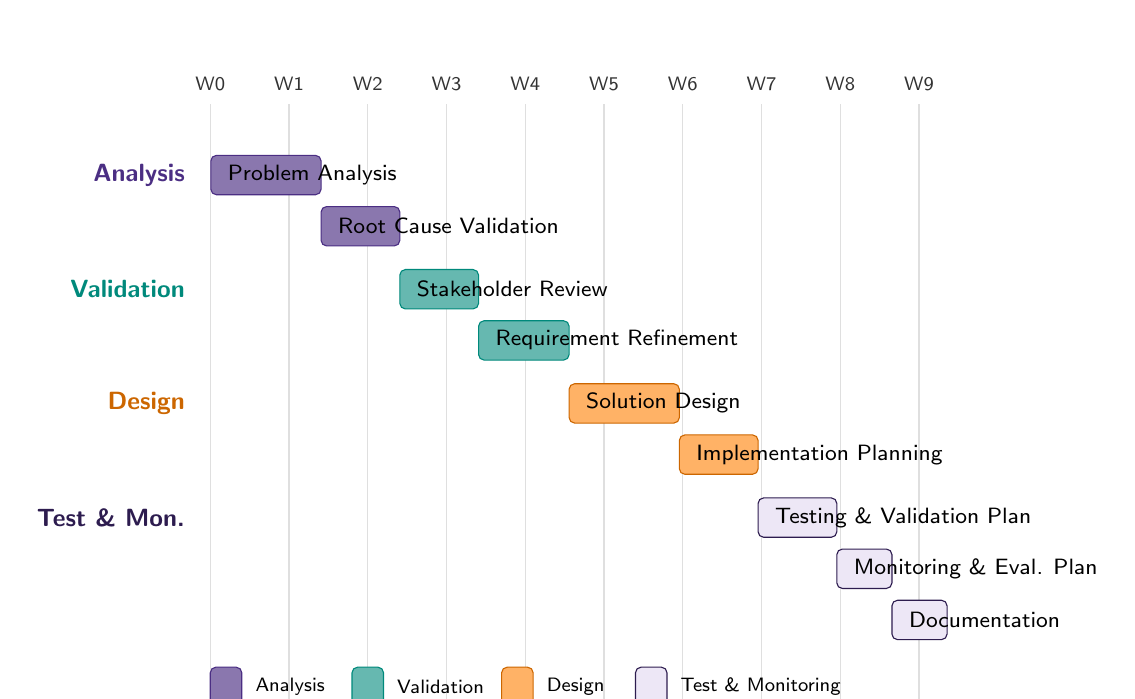
\begin{tikzpicture}[
    every node/.style={font=\sffamily\small},
    sectionlabel/.style={font=\sffamily\bfseries\small, anchor=east},
    tasklabel/.style={font=\sffamily\footnotesize, anchor=west},
    barA/.style={rectangle, rounded corners=2pt, draw=primary, fill=primary!65, minimum height=0.5cm},
    barB/.style={rectangle, rounded corners=2pt, draw=accent, fill=accent!60, minimum height=0.5cm},
    barC/.style={rectangle, rounded corners=2pt, draw=orange!80!black, fill=orange!60, minimum height=0.5cm},
    barD/.style={rectangle, rounded corners=2pt, draw=primary!60!black, fill=secondary, minimum height=0.5cm},
]
% Scale: 1 unit = 1 week. Start 2026-06-01. ~9 weeks.
\foreach \w in {0,1,...,9} {
    \draw[gray!25] (\w,0.5) -- (\w,-7.2);
    \node[font=\sffamily\scriptsize, color=darkgray, anchor=south] at (\w,0.55) {W\w};
}
% Analysis (primary)
\node[sectionlabel, color=primary] at (-0.2,-0.4) {Analysis};
\node[barA, anchor=west, minimum width=1.4cm] at (0,-0.4) {}; \node[tasklabel] at (0.1,-0.4) {Problem Analysis};
\node[barA, anchor=west, minimum width=1.0cm] at (1.4,-1.05) {}; \node[tasklabel] at (1.5,-1.05) {Root Cause Validation};
% Validation (accent)
\node[sectionlabel, color=accent] at (-0.2,-1.85) {Validation};
\node[barB, anchor=west, minimum width=1.0cm] at (2.4,-1.85) {}; \node[tasklabel] at (2.5,-1.85) {Stakeholder Review};
\node[barB, anchor=west, minimum width=1.15cm] at (3.4,-2.5) {}; \node[tasklabel] at (3.5,-2.5) {Requirement Refinement};
% Design (orange)
\node[sectionlabel, color=orange!80!black] at (-0.2,-3.3) {Design};
\node[barC, anchor=west, minimum width=1.4cm] at (4.55,-3.3) {}; \node[tasklabel] at (4.65,-3.3) {Solution Design};
\node[barC, anchor=west, minimum width=1.0cm] at (5.95,-3.95) {}; \node[tasklabel] at (6.05,-3.95) {Implementation Planning};
% Test & Monitoring (secondary)
\node[sectionlabel, color=primary!60!black] at (-0.2,-4.75) {Test \& Mon.};
\node[barD, anchor=west, minimum width=1.0cm] at (6.95,-4.75) {}; \node[tasklabel] at (7.05,-4.75) {Testing \& Validation Plan};
\node[barD, anchor=west, minimum width=0.7cm] at (7.95,-5.4) {}; \node[tasklabel] at (8.05,-5.4) {Monitoring \& Eval. Plan};
\node[barD, anchor=west, minimum width=0.7cm] at (8.65,-6.05) {}; \node[tasklabel] at (8.75,-6.05) {Documentation};
% Legend
\node[barA, minimum width=0.4cm] at (0.2,-6.9) {}; \node[anchor=west, font=\sffamily\scriptsize] at (0.45,-6.9) {Analysis};
\node[barB, minimum width=0.4cm] at (2.0,-6.9) {}; \node[anchor=west, font=\sffamily\scriptsize] at (2.25,-6.9) {Validation};
\node[barC, minimum width=0.4cm] at (3.9,-6.9) {}; \node[anchor=west, font=\sffamily\scriptsize] at (4.15,-6.9) {Design};
\node[barD, minimum width=0.4cm] at (5.6,-6.9) {}; \node[anchor=west, font=\sffamily\scriptsize] at (5.85,-6.9) {Test \& Monitoring};
\end{tikzpicture}
}
\caption{Planning Gantt Chart --- Problem 01 (Weeks from 1 June 2026)}
\end{figure}

\subsubsection{Stakeholder Engagement}
Following the problem presentation, a stakeholder validation workshop was facilitated with project managers, senior developers, and account leads.

\textbf{Validation summary.} Project managers emphasised that approvals in chat are frequently informal and often lack context (for example, missing scope boundaries or acceptance criteria). Developers reported that chat-only approvals lead to divergent interpretations of requirements, especially for multi-iteration features. Account leads observed that client confirmations are sometimes fragmented across multiple messages, which complicates billing evidence.

\textbf{Concerns raised.} Stakeholders were concerned about the administrative burden introduced by any capture mechanism that required extensive manual entry; they emphasised the need for a low-friction, one-click confirmation flow. Several team members flagged possible privacy concerns where client messages included PII, requiring controlled redaction and access restrictions. PMs, already time-constrained, requested automation to reduce manual reconciliation rather than additional tasks.

\begin{noteBox}
\textbf{Refinement to problem definition:} Based on feedback, the team refined the focus to capturing \emph{contextual approvals} (approval + scope fragment + timestamp + actor) rather than raw chat transcripts. The requirement set now includes a mandatory minimal metadata model (approval flag, requirement reference, approver identity) and an operator review queue for ambiguous items.
\end{noteBox}

\textbf{Constraints and incorporation.} Stakeholders identified WhatsApp API limitations (templates, rate limits) and occasional offline access for some clients. The planning team will include a lightweight human-in-the-loop operator flow, enforce strict PII redaction, and prioritise automation to minimise PM workload. The pilot scope will include two project teams with representative client types (local and international).

\subsubsection{Cost Management}
A high-level cost approach focuses on resource identification and control rather than detailed budgeting at this stage. Expected resources include one backend integration engineer (part-time), one frontend/UI resource for the operator confirmation UI (part-time), one QA/tester (part-time), and a 20\% allocation of a PM for stakeholder coordination. Contract costs for a WhatsApp gateway (e.g., Twilio or a managed provider) are anticipated if the managed API path is selected. Cost control strategies include using open-source integration tools where possible, limiting the pilot to two projects, and deferring expensive connectors until validated.

\subsubsection{Quality Management}
\begin{summaryBox}
\textbf{Quality objectives:} (1) capture 95\% of formal approvals related to tracked requirements during the pilot; (2) reduce approval-related clarification cycles by 50\% in pilot projects; (3) ensure no unredacted PII is stored in the canonical database.
\end{summaryBox}

\textbf{Acceptance criteria.} The pilot is accepted if the operator queue demonstrates capture accuracy above 95\% on a test sample and stakeholders confirm that captured approvals can be unambiguously linked to work items. Security acceptance requires demonstration of redaction and controlled access.

\textbf{Measurement and control.} Quality is measured through sampling and automated metrics: \texttt{capture\_rate}, \texttt{review\_resolution\_time}, and the number of PII exposures. Daily ingestion metrics and a weekly quality review are established. Mitigations for quality risks (false positives/negatives, operator backlog) include conservative confidence thresholds, a capped operator queue, and escalation rules for unresolved items.

% ----------------------------------------------------------------
% PROBLEM 02
% ----------------------------------------------------------------
\subsection{Problem 02 --- System Fragmentation \& Lack of Integration}

\textbf{Problem context.} NextStepBD currently uses multiple tools and data stores that do not communicate consistently with one another. Information often has to be copied manually from one platform to another, which increases the chance of errors, duplicate records, and missed updates. The lack of integration also makes it harder for staff to get a single, reliable view of operational information.

\subsubsection{Schedule Management}

\begin{table}[H]
\centering
\renewcommand{\arraystretch}{1.25}
\small
\begin{tabularx}{\textwidth}{|c|p{4.2cm}|X|}
\hline
\rowcolor{secondary}
\textbf{WBS} & \textbf{Work Package} & \textbf{Key Activities} \\
\hline
1.1 & Problem Analysis & Catalogue existing data stores and tools; map high-frequency cross-system workflows. \\
\hline
1.2 & Root Cause Validation & Identify barriers to integration (APIs, rate limits, workflows); prioritise integration targets by business value. \\
\hline
1.3 & Stakeholder Review & Conduct workshops with operations and finance; validate integration priorities and constraints. \\
\hline
1.4 & Requirement Refinement & Define canonical data model requirements; define connector contracts and event models. \\
\hline
1.5 & Solution Design & Design integration architecture and API contracts; define retry, queuing and error-handling strategies. \\
\hline
1.6 & Implementation Planning & Pilot connector selection and scheduling; provision queue and integration infrastructure. \\
\hline
1.7 & Testing \& Validation Planning & Integration test plan and environment design; reconciliation test cases and acceptance criteria. \\
\hline
1.8 & Monitoring \& Evaluation Planning & Define integration health KPIs; define reconciliation reporting cadence. \\
\hline
1.9 & Documentation & API contract documentation; integration runbooks and operator procedures. \\
\hline
\end{tabularx}
\caption{WBS --- Problem 02: System Fragmentation \& Lack of Integration}
\end{table}

\begin{figure}[H]
\centering
\resizebox{\textwidth}{!}{
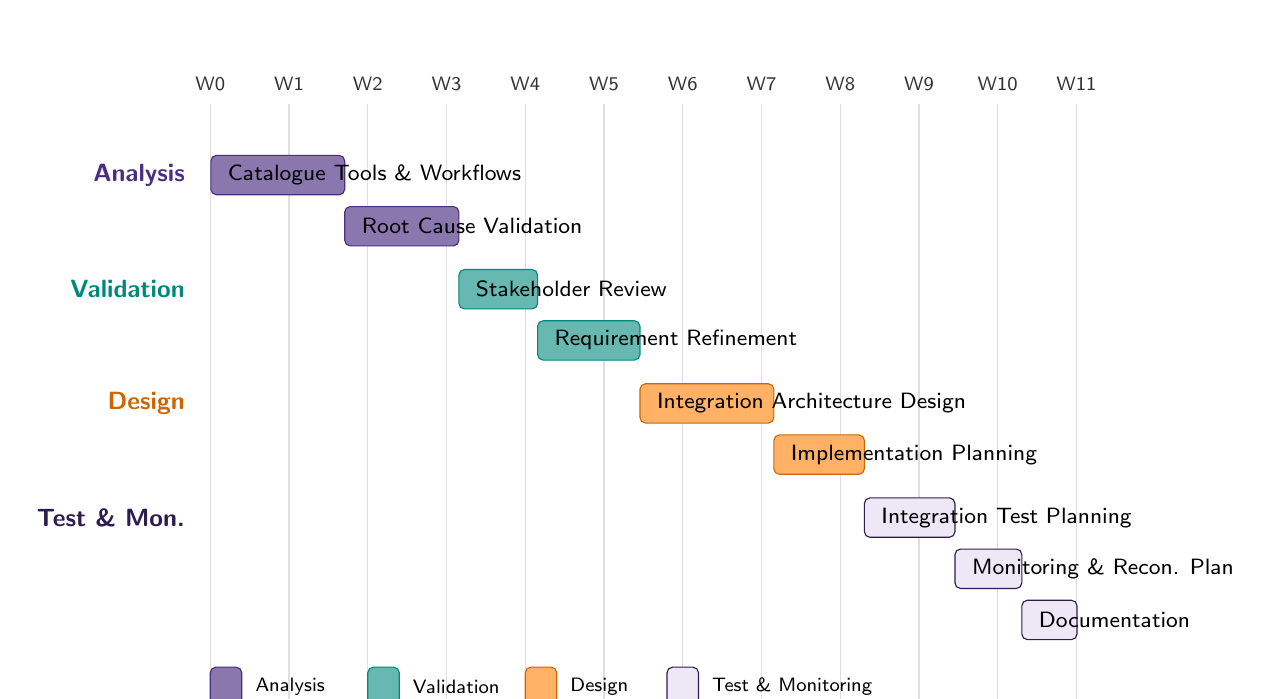
\begin{tikzpicture}[
    every node/.style={font=\sffamily\small},
    sectionlabel/.style={font=\sffamily\bfseries\small, anchor=east},
    tasklabel/.style={font=\sffamily\footnotesize, anchor=west},
    barA/.style={rectangle, rounded corners=2pt, draw=primary, fill=primary!65, minimum height=0.5cm},
    barB/.style={rectangle, rounded corners=2pt, draw=accent, fill=accent!60, minimum height=0.5cm},
    barC/.style={rectangle, rounded corners=2pt, draw=orange!80!black, fill=orange!60, minimum height=0.5cm},
    barD/.style={rectangle, rounded corners=2pt, draw=primary!60!black, fill=secondary, minimum height=0.5cm},
]
% ~11 weeks
\foreach \w in {0,1,...,11} {
    \draw[gray!25] (\w,0.5) -- (\w,-7.2);
    \node[font=\sffamily\scriptsize, color=darkgray, anchor=south] at (\w,0.55) {W\w};
}
\node[sectionlabel, color=primary] at (-0.2,-0.4) {Analysis};
\node[barA, anchor=west, minimum width=1.7cm] at (0,-0.4) {}; \node[tasklabel] at (0.1,-0.4) {Catalogue Tools \& Workflows};
\node[barA, anchor=west, minimum width=1.45cm] at (1.7,-1.05) {}; \node[tasklabel] at (1.8,-1.05) {Root Cause Validation};
\node[sectionlabel, color=accent] at (-0.2,-1.85) {Validation};
\node[barB, anchor=west, minimum width=1.0cm] at (3.15,-1.85) {}; \node[tasklabel] at (3.25,-1.85) {Stakeholder Review};
\node[barB, anchor=west, minimum width=1.3cm] at (4.15,-2.5) {}; \node[tasklabel] at (4.25,-2.5) {Requirement Refinement};
\node[sectionlabel, color=orange!80!black] at (-0.2,-3.3) {Design};
\node[barC, anchor=west, minimum width=1.7cm] at (5.45,-3.3) {}; \node[tasklabel] at (5.55,-3.3) {Integration Architecture Design};
\node[barC, anchor=west, minimum width=1.15cm] at (7.15,-3.95) {}; \node[tasklabel] at (7.25,-3.95) {Implementation Planning};
\node[sectionlabel, color=primary!60!black] at (-0.2,-4.75) {Test \& Mon.};
\node[barD, anchor=west, minimum width=1.15cm] at (8.3,-4.75) {}; \node[tasklabel] at (8.4,-4.75) {Integration Test Planning};
\node[barD, anchor=west, minimum width=0.85cm] at (9.45,-5.4) {}; \node[tasklabel] at (9.55,-5.4) {Monitoring \& Recon. Plan};
\node[barD, anchor=west, minimum width=0.7cm] at (10.3,-6.05) {}; \node[tasklabel] at (10.4,-6.05) {Documentation};
\node[barA, minimum width=0.4cm] at (0.2,-6.9) {}; \node[anchor=west, font=\sffamily\scriptsize] at (0.45,-6.9) {Analysis};
\node[barB, minimum width=0.4cm] at (2.2,-6.9) {}; \node[anchor=west, font=\sffamily\scriptsize] at (2.45,-6.9) {Validation};
\node[barC, minimum width=0.4cm] at (4.2,-6.9) {}; \node[anchor=west, font=\sffamily\scriptsize] at (4.45,-6.9) {Design};
\node[barD, minimum width=0.4cm] at (6.0,-6.9) {}; \node[anchor=west, font=\sffamily\scriptsize] at (6.25,-6.9) {Test \& Monitoring};
\end{tikzpicture}
}
\caption{Planning Gantt Chart --- Problem 02 (Weeks from 1 June 2026)}
\end{figure}

\subsubsection{Stakeholder Engagement}
Stakeholders engaged for this topic included operations leads, finance representatives, and senior engineers.

\textbf{Validation and feedback.} Operations emphasised the prevalence of unsystematic, manual reconciliation tasks consuming several person-days each month. Finance described specific reconciliation errors that had previously led to misinvoicing. Engineers identified integration constraints, including the lack of stable external IDs in some Sheets, inconsistent schema versions, and API rate limits for certain provider integrations. All parties prioritised connectors that directly reduce reconciliation labour (Sheets-to-canonical customer mapping and GitHub issue status to project trackers).

\textbf{Concerns raised.} Engineering stakeholders warned about the time required to implement robust deduplication and mapping logic, particularly for legacy Sheets with inconsistent headings. Finance requested that the canonical model preserve provenance for all data to enable auditability. Operations requested that integrations be resilient and observable to avoid silent failures.

\begin{noteBox}
\textbf{Refinement to problem definition:} The problem was refined to focus on high-value integration points and to emphasise the requirement for provenance metadata. The WBS was adjusted to include reconciliation test cases and provenance-preservation requirements.
\end{noteBox}

\textbf{Constraints and incorporation.} Constraints include unstructured spreadsheets, potential data cleansing, and API rate limits. The team will prioritise connectors that reduce manual reconciliation first, allocate a data-cleaning sprint in the pilot, and include comprehensive reconciliation reports in acceptance criteria.

\subsubsection{Cost Management}
Resource expectations focus on a small integration team: one integration engineer full-time for the pilot period, one data analyst (part-time) for mapping and cleaning, and one QA resource for integration testing. Infrastructure costs include queueing/messaging and modest compute; if a managed iPaaS is chosen, subscription fees must be budgeted. Cost control strategies include staging connectors (start with Sheets and GitHub), using open-source middleware where appropriate, and deferring expensive enterprise connectors until the central model is proven.

\subsubsection{Quality Management}
\begin{summaryBox}
\textbf{Quality objectives:} (1) successful, auditable synchronisation of core data fields for 95\% of sample records; (2) reconciliation reports generated automatically and checked weekly; (3) maintenance of provenance for all synchronised records.
\end{summaryBox}

\textbf{Acceptance and measurement.} The integration pilot must demonstrate end-to-end synchronisation for the selected connectors with clear reconciliation outputs and error-handling behaviour. Quality is measured by data synchronisation success rate, reconciliation discrepancy counts, and mean time to detect synchronisation failures. Scheduled reconciliation jobs and dashboards surface anomalies, with alerting when error thresholds are exceeded. Quality assurance includes contract tests, mock endpoint tests, and sample-based reconciliation validation.

% ----------------------------------------------------------------
% PROBLEM 03
% ----------------------------------------------------------------
\subsection{Problem 03 --- Data Management \& Governance Deficiencies}

\textbf{Problem context.} Several working records appear to be maintained in spreadsheets and informal files without a consistent data structure or ownership model. This makes it difficult to keep records accurate, track their origin, or decide which version should be treated as current. As the company grows, these weaknesses can affect reporting quality, billing accuracy, and general operational control.

\subsubsection{Schedule Management}

\begin{table}[H]
\centering
\renewcommand{\arraystretch}{1.25}
\small
\begin{tabularx}{\textwidth}{|c|p{4.2cm}|X|}
\hline
\rowcolor{secondary}
\textbf{WBS} & \textbf{Work Package} & \textbf{Key Activities} \\
\hline
1.1 & Problem Analysis & Inventory data sources and owners; identify primary inconsistencies and duplication patterns. \\
\hline
1.2 & Root Cause Validation & Trace lineage for representative records; validate ownership and custodianship responsibilities. \\
\hline
1.3 & Stakeholder Review & Hold governance workshop (finance, operations, delivery); agree minimal canonical data model and retention rules. \\
\hline
1.4 & Requirement Refinement & Define schema and mandatory fields; define provenance and retention policy requirements. \\
\hline
1.5 & Solution Design & Design canonical store and data lifecycle; specify migration and reconciliation strategy. \\
\hline
1.6 & Implementation Planning & Plan migration sprints and validation checks; define roles for data stewardship. \\
\hline
1.7 & Testing \& Validation Planning & Define migration validation tests and acceptance criteria; plan governance audits and sampling. \\
\hline
1.8 & Monitoring \& Evaluation Planning & Establish data quality KPIs (completeness, consistency); schedule periodic data quality reports. \\
\hline
1.9 & Documentation & Data dictionary and stewardship guide; retention and redaction policies. \\
\hline
\end{tabularx}
\caption{WBS --- Problem 03: Data Management \& Governance Deficiencies}
\end{table}

\begin{figure}[H]
\centering
\resizebox{\textwidth}{!}{
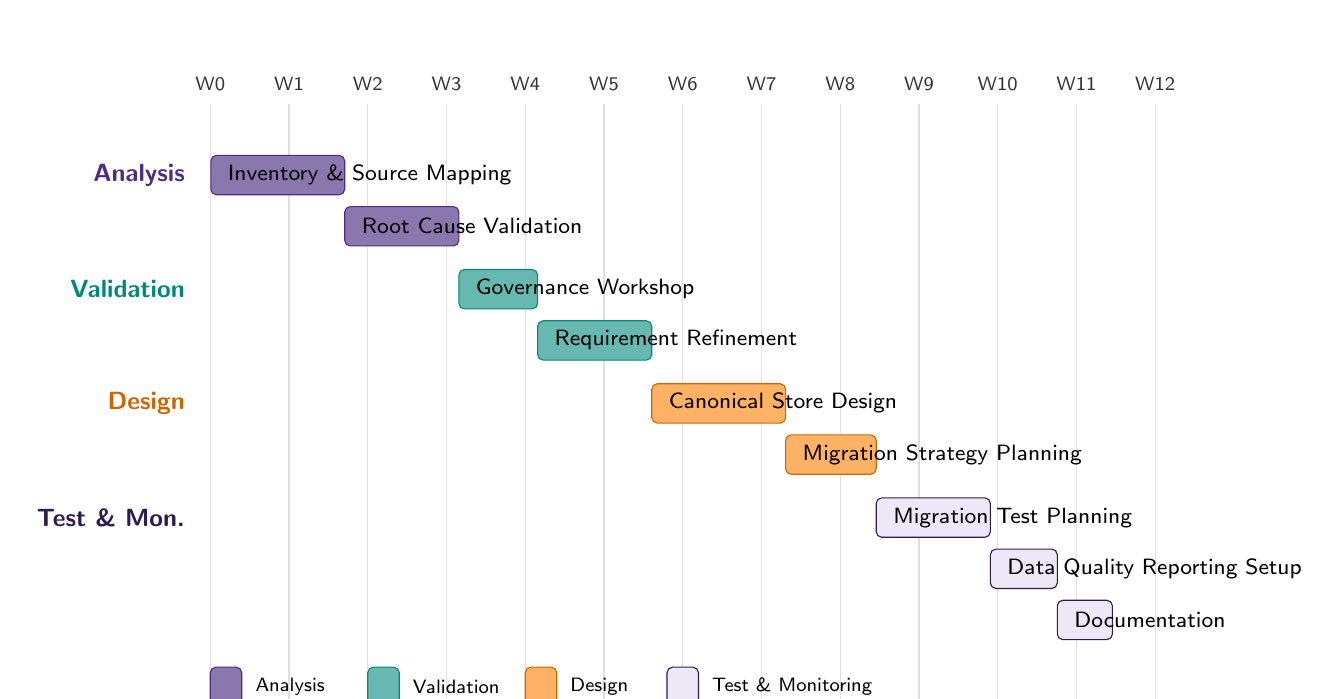
\begin{tikzpicture}[
    every node/.style={font=\sffamily\small},
    sectionlabel/.style={font=\sffamily\bfseries\small, anchor=east},
    tasklabel/.style={font=\sffamily\footnotesize, anchor=west},
    barA/.style={rectangle, rounded corners=2pt, draw=primary, fill=primary!65, minimum height=0.5cm},
    barB/.style={rectangle, rounded corners=2pt, draw=accent, fill=accent!60, minimum height=0.5cm},
    barC/.style={rectangle, rounded corners=2pt, draw=orange!80!black, fill=orange!60, minimum height=0.5cm},
    barD/.style={rectangle, rounded corners=2pt, draw=primary!60!black, fill=secondary, minimum height=0.5cm},
]
% ~12 weeks
\foreach \w in {0,1,...,12} {
    \draw[gray!25] (\w,0.5) -- (\w,-7.2);
    \node[font=\sffamily\scriptsize, color=darkgray, anchor=south] at (\w,0.55) {W\w};
}
\node[sectionlabel, color=primary] at (-0.2,-0.4) {Analysis};
\node[barA, anchor=west, minimum width=1.7cm] at (0,-0.4) {}; \node[tasklabel] at (0.1,-0.4) {Inventory \& Source Mapping};
\node[barA, anchor=west, minimum width=1.45cm] at (1.7,-1.05) {}; \node[tasklabel] at (1.8,-1.05) {Root Cause Validation};
\node[sectionlabel, color=accent] at (-0.2,-1.85) {Validation};
\node[barB, anchor=west, minimum width=1.0cm] at (3.15,-1.85) {}; \node[tasklabel] at (3.25,-1.85) {Governance Workshop};
\node[barB, anchor=west, minimum width=1.45cm] at (4.15,-2.5) {}; \node[tasklabel] at (4.25,-2.5) {Requirement Refinement};
\node[sectionlabel, color=orange!80!black] at (-0.2,-3.3) {Design};
\node[barC, anchor=west, minimum width=1.7cm] at (5.6,-3.3) {}; \node[tasklabel] at (5.7,-3.3) {Canonical Store Design};
\node[barC, anchor=west, minimum width=1.15cm] at (7.3,-3.95) {}; \node[tasklabel] at (7.4,-3.95) {Migration Strategy Planning};
\node[sectionlabel, color=primary!60!black] at (-0.2,-4.75) {Test \& Mon.};
\node[barD, anchor=west, minimum width=1.45cm] at (8.45,-4.75) {}; \node[tasklabel] at (8.55,-4.75) {Migration Test Planning};
\node[barD, anchor=west, minimum width=0.85cm] at (9.9,-5.4) {}; \node[tasklabel] at (10.0,-5.4) {Data Quality Reporting Setup};
\node[barD, anchor=west, minimum width=0.7cm] at (10.75,-6.05) {}; \node[tasklabel] at (10.85,-6.05) {Documentation};
\node[barA, minimum width=0.4cm] at (0.2,-6.9) {}; \node[anchor=west, font=\sffamily\scriptsize] at (0.45,-6.9) {Analysis};
\node[barB, minimum width=0.4cm] at (2.2,-6.9) {}; \node[anchor=west, font=\sffamily\scriptsize] at (2.45,-6.9) {Validation};
\node[barC, minimum width=0.4cm] at (4.2,-6.9) {}; \node[anchor=west, font=\sffamily\scriptsize] at (4.45,-6.9) {Design};
\node[barD, minimum width=0.4cm] at (6.0,-6.9) {}; \node[anchor=west, font=\sffamily\scriptsize] at (6.25,-6.9) {Test \& Monitoring};
\end{tikzpicture}
}
\caption{Planning Gantt Chart --- Problem 03 (Weeks from 1 June 2026)}
\end{figure}

\subsubsection{Stakeholder Engagement}
Governance workshops involved finance, delivery leads and an operations representative.

\textbf{Validation and feedback.} Finance insisted on immutable provenance records and explicit retention policies for billing-related fields. Delivery leads highlighted that imposing strict mandatory fields prematurely would block engineering work; they recommended a phased approach where a minimal viable schema is enforced initially and additional fields are gradually required. Operations asked for clear data stewardship responsibilities and a lightweight process for resolving data conflicts.

\textbf{Concerns raised.} Stakeholders were concerned about the cost and time required for large-scale data cleansing, and cautioned against governance policy that could slow legitimate work. Another concern was the potential disruption to reporting if canonicalisation changed identifiers used by external finance systems.

\begin{noteBox}
\textbf{Refinement to problem definition:} The definition was adjusted to prioritise a minimal viable canonical schema and to introduce a staged governance model (pilot $\rightarrow$ extend) to reduce initial disruption.
\end{noteBox}

\textbf{Constraints and incorporation.} Large legacy Sheets with inconsistent keys were identified as a principal constraint, with migration errors that could affect billing as a key risk. The team will allocate a data-cleaning sprint, provision a part-time data analyst, and design the migration plan with careful rollback and reconciliation checkpoints.

\subsubsection{Cost Management}
Resource needs include a data analyst (part-time), integration-engineer support for migration tooling, and a portion of the PM's time. Infrastructure may require temporary compute/storage for staging and reconciliation. Cost monitoring uses time-tracking and milestone-based controls; cost control prioritises high-impact data fields, automates cleaning where feasible, and defers low-value normalisation.

\subsubsection{Quality Management}
\begin{summaryBox}
\textbf{Quality objectives:} (1) canonical-schema completeness of mandatory fields for 90\% of migrated records in the pilot; (2) reconciliation discrepancy rate below the defined threshold; (3) documented data lineage for billing-critical records.
\end{summaryBox}

\textbf{Acceptance and measurement.} The pilot migration must pass reconciliation tests, and stakeholders must confirm the canonical representation supports required reporting. Data completeness, duplication rates, and reconciliation discrepancy counts are measured via sampling and automated checks. Weekly data-quality reports and escalation handle unresolved discrepancies. Mitigations for quality risks (irreversible data loss, legacy identifier mismatches) include snapshot backups, staged migration, and migration dry-runs with pre-defined reconciliation scripts.

% ----------------------------------------------------------------
% PROBLEM 04
% ----------------------------------------------------------------
\subsection{Problem 04 --- Security \& Access Control Risks}

\textbf{Problem context.} Some operational information appears to move across tools with limited access control and limited audit visibility. This can lead to inconsistent handling of sensitive data, unclear responsibility for access decisions, and greater exposure if an account is shared or compromised. A more controlled approach is needed so that sensitive records can be handled with clearer rules and better traceability.

\subsubsection{Schedule Management}

\begin{table}[H]
\centering
\renewcommand{\arraystretch}{1.25}
\small
\begin{tabularx}{\textwidth}{|c|p{4.2cm}|X|}
\hline
\rowcolor{secondary}
\textbf{WBS} & \textbf{Work Package} & \textbf{Key Activities} \\
\hline
1.1 & Problem Analysis & Inventory channels and typical PII exposures; review current access-control practices and gaps. \\
\hline
1.2 & Root Cause Validation & Identify processes that allow credential sharing; map regulatory/compliance obligations. \\
\hline
1.3 & Stakeholder Review & Consult legal, operations and client-facing roles; validate risk appetite and policy priorities. \\
\hline
1.4 & Requirement Refinement & Define RBAC model requirements and SSO needs; define PII handling and redaction rules. \\
\hline
1.5 & Solution Design & Design authentication and authorisation architecture; define audit logging and retention specifications. \\
\hline
1.6 & Implementation Planning & Plan SSO/RBAC integration and secret management; prepare access-control test plan. \\
\hline
1.7 & Testing \& Validation Planning & Define security acceptance tests and penetration checks; define audit review schedules. \\
\hline
1.8 & Monitoring \& Evaluation Planning & Define audit-log monitoring KPIs; define incident detection and response plan. \\
\hline
1.9 & Documentation & Security policy and role matrix; incident response and redaction guides. \\
\hline
\end{tabularx}
\caption{WBS --- Problem 04: Security \& Access Control Risks}
\end{table}

\begin{figure}[H]
\centering
\resizebox{\textwidth}{!}{
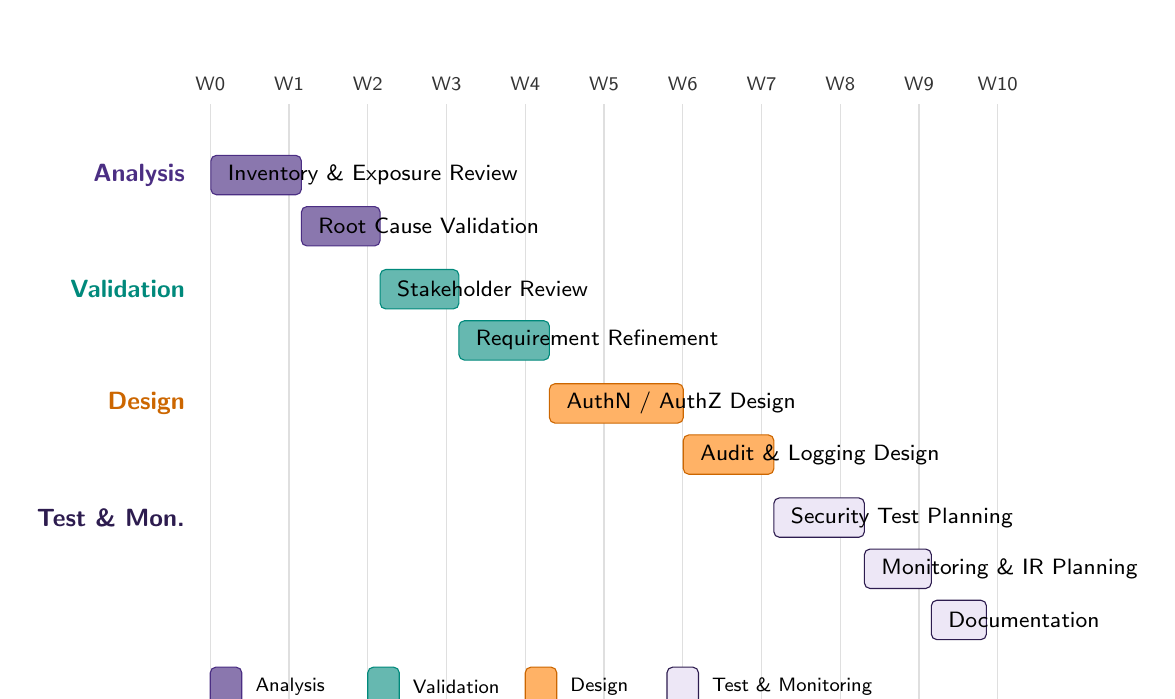
\begin{tikzpicture}[
    every node/.style={font=\sffamily\small},
    sectionlabel/.style={font=\sffamily\bfseries\small, anchor=east},
    tasklabel/.style={font=\sffamily\footnotesize, anchor=west},
    barA/.style={rectangle, rounded corners=2pt, draw=primary, fill=primary!65, minimum height=0.5cm},
    barB/.style={rectangle, rounded corners=2pt, draw=accent, fill=accent!60, minimum height=0.5cm},
    barC/.style={rectangle, rounded corners=2pt, draw=orange!80!black, fill=orange!60, minimum height=0.5cm},
    barD/.style={rectangle, rounded corners=2pt, draw=primary!60!black, fill=secondary, minimum height=0.5cm},
]
% ~9.5 weeks
\foreach \w in {0,1,...,10} {
    \draw[gray!25] (\w,0.5) -- (\w,-7.2);
    \node[font=\sffamily\scriptsize, color=darkgray, anchor=south] at (\w,0.55) {W\w};
}
\node[sectionlabel, color=primary] at (-0.2,-0.4) {Analysis};
\node[barA, anchor=west, minimum width=1.15cm] at (0,-0.4) {}; \node[tasklabel] at (0.1,-0.4) {Inventory \& Exposure Review};
\node[barA, anchor=west, minimum width=1.0cm] at (1.15,-1.05) {}; \node[tasklabel] at (1.25,-1.05) {Root Cause Validation};
\node[sectionlabel, color=accent] at (-0.2,-1.85) {Validation};
\node[barB, anchor=west, minimum width=1.0cm] at (2.15,-1.85) {}; \node[tasklabel] at (2.25,-1.85) {Stakeholder Review};
\node[barB, anchor=west, minimum width=1.15cm] at (3.15,-2.5) {}; \node[tasklabel] at (3.25,-2.5) {Requirement Refinement};
\node[sectionlabel, color=orange!80!black] at (-0.2,-3.3) {Design};
\node[barC, anchor=west, minimum width=1.7cm] at (4.3,-3.3) {}; \node[tasklabel] at (4.4,-3.3) {AuthN / AuthZ Design};
\node[barC, anchor=west, minimum width=1.15cm] at (6.0,-3.95) {}; \node[tasklabel] at (6.1,-3.95) {Audit \& Logging Design};
\node[sectionlabel, color=primary!60!black] at (-0.2,-4.75) {Test \& Mon.};
\node[barD, anchor=west, minimum width=1.15cm] at (7.15,-4.75) {}; \node[tasklabel] at (7.25,-4.75) {Security Test Planning};
\node[barD, anchor=west, minimum width=0.85cm] at (8.3,-5.4) {}; \node[tasklabel] at (8.4,-5.4) {Monitoring \& IR Planning};
\node[barD, anchor=west, minimum width=0.7cm] at (9.15,-6.05) {}; \node[tasklabel] at (9.25,-6.05) {Documentation};
\node[barA, minimum width=0.4cm] at (0.2,-6.9) {}; \node[anchor=west, font=\sffamily\scriptsize] at (0.45,-6.9) {Analysis};
\node[barB, minimum width=0.4cm] at (2.2,-6.9) {}; \node[anchor=west, font=\sffamily\scriptsize] at (2.45,-6.9) {Validation};
\node[barC, minimum width=0.4cm] at (4.2,-6.9) {}; \node[anchor=west, font=\sffamily\scriptsize] at (4.45,-6.9) {Design};
\node[barD, minimum width=0.4cm] at (6.0,-6.9) {}; \node[anchor=west, font=\sffamily\scriptsize] at (6.25,-6.9) {Test \& Monitoring};
\end{tikzpicture}
}
\caption{Planning Gantt Chart --- Problem 04 (Weeks from 1 June 2026)}
\end{figure}

\subsubsection{Stakeholder Engagement}
Security planning workshops were held with legal counsel (internal or external), operations, and client-facing leads.

\textbf{Validation and feedback.} Legal counsel recommended conservative retention and explicit conditions for unredaction, noting potential client contractual obligations. Operations requested pragmatic retention intervals and fast, auditable redaction procedures. Delivery leads noted the need to avoid over-restrictive access that would interfere with urgent support activities.

\textbf{Concerns raised.} Stakeholders were concerned about the complexity of retrofitting SSO and RBAC into disparate legacy tools (for example, Google Sheets and WhatsApp), emphasising the need for a phased approach and documented exceptions. Another concern was the potential increase in support tickets resulting from new access controls.

\begin{noteBox}
\textbf{Refinement to problem definition:} The team prioritised audit logging, SSO for internal systems, and production secrets management as first-order items; full SSO for external client communications was deferred pending provider support.
\end{noteBox}

\textbf{Constraints and incorporation.} Constraints include limitations of third-party messaging platforms for access control and the need to manage exceptions where SSO is not possible. The plan integrates lightweight SSO for internal systems and vault-based secrets management; redaction workflows and audit reviews are built into pilot acceptance criteria.

\subsubsection{Cost Management}
Resource expectations include security-architect advisory time (part-time), an identity-provider subscription (if a managed SSO is used), and engineering time to integrate SSO and secrets management. Cost monitoring captures licence and integration effort; control is exercised by phasing upgrades and evaluating trade-offs between managed and self-hosted solutions.

\subsubsection{Quality Management}
\begin{summaryBox}
\textbf{Quality objectives:} (1) audit logging for critical operations with 100\% coverage of canonical record changes in the pilot; (2) a demonstrated controlled redaction/unredaction process; (3) RBAC for internal systems with role definitions and logging.
\end{summaryBox}

\textbf{Acceptance and measurement.} Audit logs must be available for review and role-based policies validated through test cases; redaction and unredaction require appropriate approvals and are recorded. Audit completeness, the number of redaction incidents, and role-assignment accuracy are measured, and security testing includes basic penetration checks and role-misconfiguration tests. Continuous monitoring of audit logs and scheduled audits provide ongoing control; quality control validates log integrity and role enforcement during pilot exercises.

% ----------------------------------------------------------------
% PROBLEM 05
% ----------------------------------------------------------------
\subsection{Problem 05 --- Scalability \& Operational Bottlenecks}

\textbf{Problem context.} As the company takes on more projects, a number of routine tasks still depend on a few key individuals and manual follow-up. This can slow onboarding, make task assignment inconsistent, and create bottlenecks when staff are unavailable. Without better process support, these issues can limit the organisation's ability to grow smoothly.

\subsubsection{Schedule Management}

\begin{table}[H]
\centering
\renewcommand{\arraystretch}{1.25}
\small
\begin{tabularx}{\textwidth}{|c|p{4.2cm}|X|}
\hline
\rowcolor{secondary}
\textbf{WBS} & \textbf{Work Package} & \textbf{Key Activities} \\
\hline
1.1 & Problem Analysis & Map recurring bottlenecks and single-person dependencies; measure onboarding time and common failure modes. \\
\hline
1.2 & Root Cause Validation & Trace process steps that require manual PM intervention; validate capacity constraints and staff time allocation. \\
\hline
1.3 & Stakeholder Review & Workshop with HR, PMs and team leads; validate training and capacity-planning needs. \\
\hline
1.4 & Requirement Refinement & Define templates and automation requirements; define onboarding checklist and competency criteria. \\
\hline
1.5 & Solution Design & Design automation flows (auto-assignment, escalation); design onboarding materials and micro-training modules. \\
\hline
1.6 & Implementation Planning & Prepare pilot automation rules and metrics; define training schedule and mentors. \\
\hline
1.7 & Testing \& Validation Planning & Define pilot evaluation metrics (throughput, cycle time); plan user acceptance tests and training feedback sessions. \\
\hline
1.8 & Monitoring \& Evaluation Planning & Establish throughput and cycle-time KPIs; define retention and workload monitoring. \\
\hline
1.9 & Documentation & Onboarding guides and templates; process playbooks and escalation paths. \\
\hline
\end{tabularx}
\caption{WBS --- Problem 05: Scalability \& Operational Bottlenecks}
\end{table}

\begin{figure}[H]
\centering
\resizebox{\textwidth}{!}{
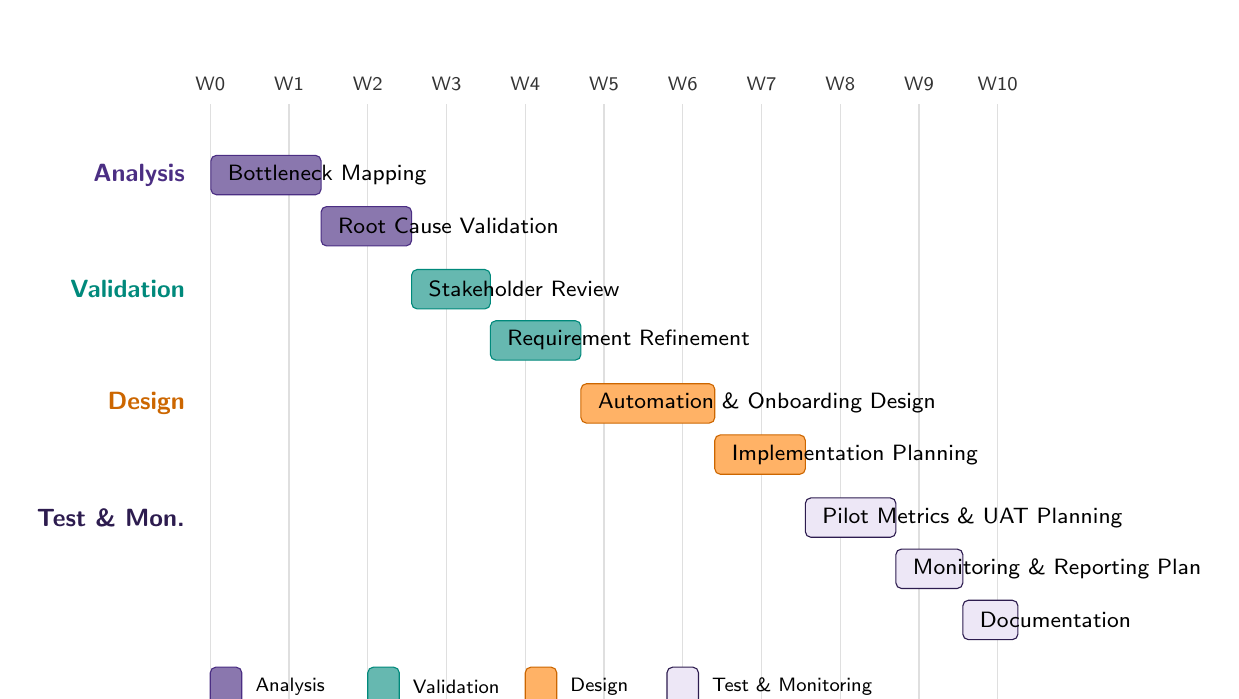
\begin{tikzpicture}[
    every node/.style={font=\sffamily\small},
    sectionlabel/.style={font=\sffamily\bfseries\small, anchor=east},
    tasklabel/.style={font=\sffamily\footnotesize, anchor=west},
    barA/.style={rectangle, rounded corners=2pt, draw=primary, fill=primary!65, minimum height=0.5cm},
    barB/.style={rectangle, rounded corners=2pt, draw=accent, fill=accent!60, minimum height=0.5cm},
    barC/.style={rectangle, rounded corners=2pt, draw=orange!80!black, fill=orange!60, minimum height=0.5cm},
    barD/.style={rectangle, rounded corners=2pt, draw=primary!60!black, fill=secondary, minimum height=0.5cm},
]
% ~10 weeks
\foreach \w in {0,1,...,10} {
    \draw[gray!25] (\w,0.5) -- (\w,-7.2);
    \node[font=\sffamily\scriptsize, color=darkgray, anchor=south] at (\w,0.55) {W\w};
}
\node[sectionlabel, color=primary] at (-0.2,-0.4) {Analysis};
\node[barA, anchor=west, minimum width=1.4cm] at (0,-0.4) {}; \node[tasklabel] at (0.1,-0.4) {Bottleneck Mapping};
\node[barA, anchor=west, minimum width=1.15cm] at (1.4,-1.05) {}; \node[tasklabel] at (1.5,-1.05) {Root Cause Validation};
\node[sectionlabel, color=accent] at (-0.2,-1.85) {Validation};
\node[barB, anchor=west, minimum width=1.0cm] at (2.55,-1.85) {}; \node[tasklabel] at (2.65,-1.85) {Stakeholder Review};
\node[barB, anchor=west, minimum width=1.15cm] at (3.55,-2.5) {}; \node[tasklabel] at (3.65,-2.5) {Requirement Refinement};
\node[sectionlabel, color=orange!80!black] at (-0.2,-3.3) {Design};
\node[barC, anchor=west, minimum width=1.7cm] at (4.7,-3.3) {}; \node[tasklabel] at (4.8,-3.3) {Automation \& Onboarding Design};
\node[barC, anchor=west, minimum width=1.15cm] at (6.4,-3.95) {}; \node[tasklabel] at (6.5,-3.95) {Implementation Planning};
\node[sectionlabel, color=primary!60!black] at (-0.2,-4.75) {Test \& Mon.};
\node[barD, anchor=west, minimum width=1.15cm] at (7.55,-4.75) {}; \node[tasklabel] at (7.65,-4.75) {Pilot Metrics \& UAT Planning};
\node[barD, anchor=west, minimum width=0.85cm] at (8.7,-5.4) {}; \node[tasklabel] at (8.8,-5.4) {Monitoring \& Reporting Plan};
\node[barD, anchor=west, minimum width=0.7cm] at (9.55,-6.05) {}; \node[tasklabel] at (9.65,-6.05) {Documentation};
\node[barA, minimum width=0.4cm] at (0.2,-6.9) {}; \node[anchor=west, font=\sffamily\scriptsize] at (0.45,-6.9) {Analysis};
\node[barB, minimum width=0.4cm] at (2.2,-6.9) {}; \node[anchor=west, font=\sffamily\scriptsize] at (2.45,-6.9) {Validation};
\node[barC, minimum width=0.4cm] at (4.2,-6.9) {}; \node[anchor=west, font=\sffamily\scriptsize] at (4.45,-6.9) {Design};
\node[barD, minimum width=0.4cm] at (6.0,-6.9) {}; \node[anchor=west, font=\sffamily\scriptsize] at (6.25,-6.9) {Test \& Monitoring};
\end{tikzpicture}
}
\caption{Planning Gantt Chart --- Problem 05 (Weeks from 1 June 2026)}
\end{figure}

\subsubsection{Stakeholder Engagement}
Stakeholder discussions involved HR, PMs and delivery leads.

\textbf{Validation and feedback.} HR indicated that current onboarding typically requires 4--6 weeks to reach productive contribution and that a structured checklist and mentor program could reduce this by at least two weeks. Project managers advised that many routine assignments are decided by habit and that an explicit skills inventory with capacity tagging would enable automated assignment without excessive friction. Delivery leads requested careful control of automated escalation to avoid noisy notifications.

\textbf{Concerns raised.} Stakeholders were concerned about the burden of maintaining a skills inventory and hesitated about overly prescriptive automation that might misassign complex tasks. There were also concerns about training bandwidth for mentors.

\begin{noteBox}
\textbf{Refinement to problem definition:} The solution was refined to emphasise automated support for routine assignment only, with manual override for complex cases. Onboarding improvements were specified as checklist-driven micro-training modules that complement mentoring rather than replace it.
\end{noteBox}

\textbf{Constraints and incorporation.} Constraints include limited HR capacity for mentoring and potential resistance from senior staff to automated assignment. The plan incorporates a lightweight skills-tagging template, a mentoring roster, and a limited-scope pilot; metrics collected during the pilot will drive further automation.

\subsubsection{Cost Management}
Anticipated resources include training-content development (one instructional designer or contractor), part-time mentor allocations from senior staff, and engineering time to implement automation templates and reporting. Cost control measures include reusing existing documentation where possible and prioritising micro-training over full course development.

\subsubsection{Quality Management}
\begin{summaryBox}
\textbf{Quality objectives:} (1) reduce average onboarding time by a measurable amount in the pilot; (2) ensure automated-assignment accuracy for routine tasks meets an acceptable threshold (e.g., 90\%); (3) maintain staff satisfaction as measured by post-pilot surveys.
\end{summaryBox}

\textbf{Acceptance and measurement.} The pilot must demonstrate improved onboarding metrics and acceptable assignment accuracy without degrading staff satisfaction. Onboarding time, cycle-time for routine tasks, assignment-correction rate, and staff-satisfaction survey results are captured. Weekly pilot reviews drive corrective actions for misassignment patterns and refinement of skills tags. Mitigations for quality risks (misassignment, staff pushback) include manual override, a visible audit trail for assignment decisions, and an opt-in period for affected teams.

\section{Conclusion}
This chapter converts the findings from Chapters 1 and 2 into a practical planning framework. For each problem the project team has produced a Work Breakdown Structure (WBS), a planning-focused Gantt chart, a record of stakeholder feedback, and high-level cost and quality approaches. The focus is on preparing pilots and validation activities that reduce risk and keep disruption to a minimum. Successful system development depends not only on technical feasibility but also on careful planning, stakeholder involvement, and a realistic, staged implementation strategy --- principles that carry forward into the system modelling and design work of the following chapters.

% ================================================================
% END OF CHAPTER 3
% ================================================================


% ================================================================
% START OF CHAPTER 4 — Analysis
% ================================================================
\chapter{Analysis}

\section{Introduction}
The primary purpose of this chapter is to present a comprehensive analysis of the existing operational environment at NextStepBD. Before designing a new system, it is essential to obtain a total understanding of the company's current practices, processes, capabilities, and challenges. To achieve this, a structured information-gathering strategy was formulated and executed. The findings from these activities allow for a robust assessment of business requirements and system constraints. Reviewing historical records, understanding operating procedures, and engaging stakeholders form the foundation for defining project scope and designing viable solutions.

\section{Information Gathering}
Effective information gathering serves as the baseline for accurate system analysis. The analysis employed a multi-faceted approach to gather both qualitative and quantitative insights. This phase includes reviewing existing literature, standard operating procedures, and business forms, which lay the groundwork for subsequent on-site observations, interviews, and structured questionnaires to validate and expand upon the initial findings.

\subsection{Review of Literature, Procedure and Forms}
This preliminary phase involves examining documented evidence of how NextStepBD operates. By analysing the company's publicly available literature, internal process guidelines, and the forms used to capture business data, we identify the baseline state of operations and highlight workflow gaps. Document analysis is frequently used during requirement elicitation to understand the current state before moving to the desired future state.

\subsubsection{Review of Literature}
A review of the company's official website and public literature reveals that NextStepBD operates with over a decade of service excellence, transitioning from a core software development team to a prominent provider of scalable, AI-powered enterprise solutions. Their external product portfolio features Voice AI Agents supporting multiple languages, Omnichannel Platforms for customer engagement, WhatsApp Marketing Managers, and HealthTech AI assistants. Beyond software products, they provide full-service enterprise development and creative content solutions to a vast global market. Their literature emphasises attributes like rapid deployment, enterprise-grade security, broad digital reach, and seamless integration capabilities, successfully serving hundreds of industry-leading enterprise clients. However, contrasting this outward technical maturity with internal documents reveals a paradox: while their client-facing solutions are highly automated, their internal operations face scaling challenges and fragmentation due to rapid organisational growth.

\subsubsection{Review of Procedures}
An examination of NextStepBD's internal operating procedures highlights workflows that remain heavily dependent on manual coordination. Beyond core technical operations, business handling procedures also reflect informal processing:

\begin{itemize}[leftmargin=2em]
    \item \textbf{Client Requirement Elicitation:} Initial client requirements and feature requests are predominantly gathered via informal channels such as WhatsApp or email threads. These requests are manually extrapolated into work items by Project Managers without formal sign-offs, frequently leading to scope ambiguity.
    \item \textbf{Development Process:} The development workflow begins with project managers manually assigning tasks to developers, with code generation and versioning handled via GitHub. However, the process suffers from limited internal documentation, informal peer review practices, and the absence of a standardised, automated development pipeline.
    \item \textbf{Quality Assurance and Testing:} Testing is largely ad-hoc, mostly performed directly by developers or Project Managers instead of a dedicated QA workflow. Without systematic test plan coverage, code stability occasionally suffers before production deployment.
    \item \textbf{Deployment Process:} Once code is finalised, team leads manually review it before deployment. The deployment itself relies largely on manual execution and explicit verbal or chat-based approvals rather than an automated Continuous Integration/Continuous Deployment (CI/CD) pipeline. Finally, client notifications are communicated manually via WhatsApp or email.
    \item \textbf{Billing and Invoicing:} Invoicing relies heavily on manual reconciliation. Project Managers compile completed features from disparate Google Sheets, and invoices are manually generated in Excel. Delivery of invoices and tracking of payments is handled through individual emails, creating delays and occasional discrepancies due to human error.
    \item \textbf{Customer Support \& Incident Management:} Post-deployment bug reports and support requests bypass a formal ticketing system, routing directly to developers or managers via chat. Resolution tracking is unstructured, making it difficult to analyse historical defect rates or enforce performance SLAs.
\end{itemize}

The following diagrams illustrate the informal nature of the current core operations, highlighting the central bottlenecks and manual dependencies.

\begin{figure}[H]
\centering
\resizebox{0.7\textwidth}{!}{
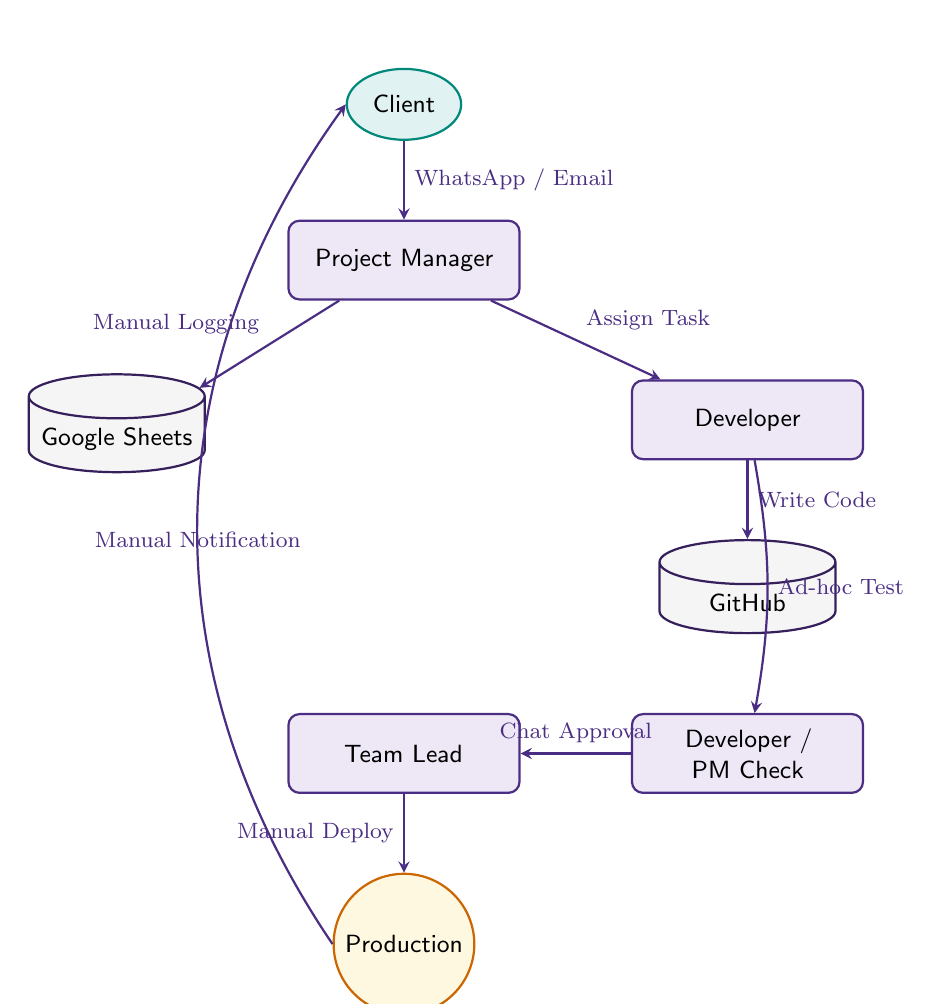
\begin{tikzpicture}[
    every node/.style={font=\sffamily\small},
    node distance=1.0cm and 1.4cm,
    actor/.style={ellipse, draw=accent, fill=softteal, thick, minimum height=0.9cm, align=center},
    proc/.style={rectangle, rounded corners, draw=primary, fill=secondary, thick, text width=2.7cm, align=center, minimum height=1.0cm},
    store/.style={cylinder, shape border rotate=90, aspect=0.25, draw=primary!70!black, fill=softgray, thick, text width=2.0cm, align=center, minimum height=1.0cm},
    prod/.style={circle, draw=orange!80!black, fill=softcream, thick, align=center, minimum size=1.4cm},
    arrow/.style={->, >=stealth, thick, color=primary}
]
\node[actor] (client) {Client};
\node[proc, below=of client] (pm) {Project Manager};
\node[store, below left=of pm] (sheets) {Google Sheets};
\node[proc, below right=of pm] (dev) {Developer};
\node[store, below=of dev] (gh) {GitHub};
\node[proc, below=1.0cm of gh] (qa) {Developer / PM Check};
\node[proc, left=of qa] (tl) {Team Lead};
\node[prod, below=of tl] (prod) {Production};

\draw[arrow] (client) -- node[right, font=\footnotesize] {WhatsApp / Email} (pm);
\draw[arrow] (pm) -- node[above left, font=\footnotesize] {Manual Logging} (sheets);
\draw[arrow] (pm) -- node[above right, font=\footnotesize] {Assign Task} (dev);
\draw[arrow] (dev) -- node[right, font=\footnotesize] {Write Code} (gh);
\draw[arrow] (dev) to[bend left=10] node[right, font=\footnotesize] {Ad-hoc Test} (qa);
\draw[arrow] (qa) -- node[above, font=\footnotesize] {Chat Approval} (tl);
\draw[arrow] (tl) -- node[left, font=\footnotesize] {Manual Deploy} (prod);
\draw[arrow] (prod.west) to[bend left=35] node[below, font=\footnotesize] {Manual Notification} (client.west);
\end{tikzpicture}
}
\caption{Current Engineering \& Delivery Workflow}
\end{figure}

\begin{figure}[H]
\centering
\resizebox{\textwidth}{!}{
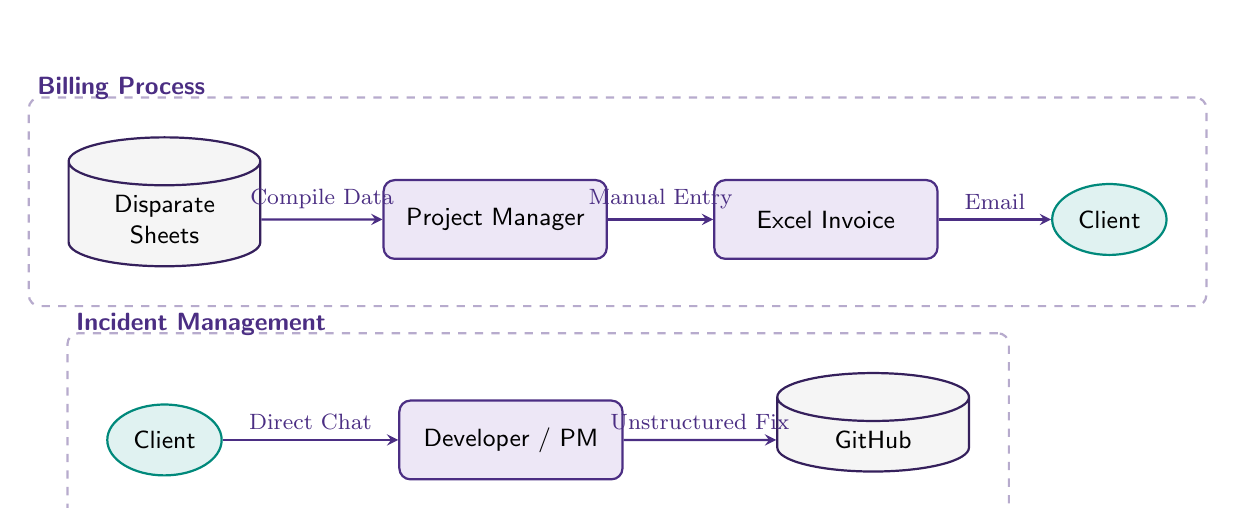
\begin{tikzpicture}[
    every node/.style={font=\sffamily\small},
    actor/.style={ellipse, draw=accent, fill=softteal, thick, minimum height=0.9cm, align=center},
    proc/.style={rectangle, rounded corners, draw=primary, fill=secondary, thick, text width=2.6cm, align=center, minimum height=1.0cm},
    store/.style={cylinder, shape border rotate=90, aspect=0.25, draw=primary!70!black, fill=softgray, thick, text width=2.2cm, align=center, minimum height=1.0cm},
    grp/.style={draw=primary!40, dashed, thick, rounded corners, inner sep=14pt},
    arrow/.style={->, >=stealth, thick, color=primary}
]
% --- Billing subgraph ---
\node[store] (s2) at (0,0) {Disparate Sheets};
\node[proc] (pm2) at (4.2,0) {Project Manager};
\node[proc] (xl) at (8.4,0) {Excel Invoice};
\node[actor] (c2) at (12.0,0) {Client};
\draw[arrow] (s2) -- node[above, font=\footnotesize] {Compile Data} (pm2);
\draw[arrow] (pm2) -- node[above, font=\footnotesize] {Manual Entry} (xl);
\draw[arrow] (xl) -- node[above, font=\footnotesize] {Email} (c2);

% --- Incident subgraph ---
\node[actor] (c3) at (0,-2.8) {Client};
\node[proc] (sup) at (4.4,-2.8) {Developer / PM};
\node[store] (gh2) at (9.0,-2.8) {GitHub};
\draw[arrow] (c3) -- node[above, font=\footnotesize] {Direct Chat} (sup);
\draw[arrow] (sup) -- node[above, font=\footnotesize] {Unstructured Fix} (gh2);

% --- Group boxes ---
\begin{pgfonlayer}{background}
    \node[grp, fit=(s2)(pm2)(xl)(c2)] (gB) {};
    \node[grp, fit=(c3)(sup)(gh2)] (gI) {};
\end{pgfonlayer}
\node[font=\sffamily\bfseries\small, color=primary, anchor=west] at (gB.north west) [yshift=3pt] {Billing Process};
\node[font=\sffamily\bfseries\small, color=primary, anchor=west] at (gI.north west) [yshift=3pt] {Incident Management};
\end{tikzpicture}
}
\caption{Current Billing and Support Workflows}
\end{figure}

While these procedures offer a high degree of situational flexibility, they create significant bottlenecks. The reliance on manual approvals, lack of automated workflows, and informal quality checks restrict operational scalability and introduce heavy dependencies on specific personnel.

\subsubsection{Review of Forms}
NextStepBD primarily utilises unstructured spreadsheets (such as Google Sheets and Microsoft Excel) instead of dedicated, relational database forms for their internal record-keeping. Handling core entity data through static, multi-authored files heavily risks data integrity, creating vulnerabilities and duplications.

The table below summarises the critical forms analysed, their current medium, and the identified operational gaps.

\begin{table}[H]
\centering
\renewcommand{\arraystretch}{1.35}
\small
\begin{tabularx}{\textwidth}{|p{2.6cm}|X|p{2.3cm}|X|}
\hline
\rowcolor{secondary}
\textbf{Form / Record Type} & \textbf{Purpose} & \textbf{Current Format} & \textbf{Limitations \& Gaps} \\
\hline
\textbf{Customer Records} & Capture client identification, contacts, and contract histories. & Disparate Excel / Google Sheets & No centralised repository; high data duplication; poor access control for sensitive data. \\
\hline
\textbf{Employee Setup \& Skills} & Track developer profiles, competencies, and system access rights. & Flat Spreadsheets & Lacks integration with task assignments; difficult to query for capacity planning. \\
\hline
\textbf{Task Assignment Form} & Allocate project work, track deadlines, and monitor completion statuses. & WhatsApp messages / Google Sheets & Highly informal; lacks automated reminders, time-tracking, and dependency mapping. \\
\hline
\textbf{Performance Review} & Evaluate employee efficiency and track historical appraisal data. & Word Documents / Printed PDFs & Not systematically integrated with daily task execution records; stored in isolated drives. \\
\hline
\textbf{Billing \& Invoice Form} & Bill clients for completed milestones or retainer periods. & Manual Excel Templates & Requires manual cross-referencing with task sheets; prone to calculation and tracking errors. \\
\hline
\textbf{Incident / Support Ticket} & Log bugs, system failures, and feature requests post-deployment. & Email threads \& Chat Logs & No standardised intake form; difficult to track resolution times, SLAs, or defect trends. \\
\hline
\end{tabularx}
\caption{Analysis of Critical Forms, Current Medium, and Operational Gaps}
\end{table}

\subsection{On Site Observation}
Due to scheduling constraints, the prevalence of remote and hybrid work models adopted by the team, and confidentiality requirements for ongoing projects, conducting a formal, prolonged on-site observation of the workflows was not possible for this study. Instead, the analysis relies more heavily on self-reported data through interviews and questionnaires, as well as the documentation analysis provided above.

\subsection{Interview}
To gain a deeper, qualitative understanding of the operational challenges, semi-structured interviews were conducted with key stakeholders across NextStepBD. These interviews helped identify unwritten rules, cultural pain points, and specific areas where the informal systems are failing to scale.

% Custom list style for interview Q&A
% (uses description-like layout)
\newcommand{\interviewQ}[1]{\vspace{2pt}\noindent\textbf{Q: #1}\par}
\newcommand{\interviewA}[1]{\noindent\textit{A:}~#1\par\vspace{4pt}}

\subsubsection{Interview with CEO}
\interviewQ{Can you describe the company's current strategic priorities for the next 12--24 months?}
\interviewA{Over the next year or two, our primary focus is strengthening recurring revenue streams while improving the predictability and quality of delivery. Practically, this means investing selectively in tools and process improvements that reduce rework and late deliveries, piloting automation to relieve project managers of repetitive reconciliation tasks, and packaging a small set of services into repeatable product offerings that generate steadier income. We are conscious of cost and time-to-value, so early pilots should deliver measurable operational benefits within a few months.}
\interviewQ{What are the most important operational risks you see today?}
\interviewA{The most pressing risks are fragmented information flows that lead to misaligned scope and billing, single-person knowledge dependencies, and the use of informal channels for sensitive client data. Fragmented records create disputes that take time to resolve and harm client trust; key-person dependencies create single points of failure when staff leave or are unavailable; and informal handling of PII or credentials raises legal and reputational exposure. Mitigations should therefore focus on reliable capture of approvals, shared knowledge practices, and stronger access controls.}
\interviewQ{How do you measure service delivery success and client satisfaction?}
\interviewA{We track a mix of operational and customer-facing indicators: on-time delivery rates, a basic client satisfaction check after each engagement, the volume and severity of billing disputes, and the time PMs spend on reconciliation activities. Qualitative feedback from account leads also informs our assessment, especially where repeated clarifications or churn indicate deeper process issues. Over time I'd like these measures to be automated or surfaced on dashboards so we can act faster.}
\interviewQ{Which processes or tools do you think limit the company's ability to scale?}
\interviewA{Reliance on spreadsheets and chat for approvals and record-keeping is a major limiter. Without canonical identifiers for clients and contracts and a reliable capture mechanism for approvals, we add headcount to preserve consistency rather than improving efficiency. Likewise, tools that require duplicate entry or do not integrate well force manual reconciliation work that does not scale.}
\interviewQ{How are decisions about investment in tools, integrations, and people made?}
\interviewA{Decisions are made by weighing ROI against time-to-value and risk. For urgent pain points we prefer low-friction SaaS pilots to prove value quickly; for structural capabilities or compliance needs we consider funded internal or custom work. Larger expenditures typically require a sponsor-level approval and a clear business case showing cost savings or revenue protection.}
\interviewQ{How do you currently obtain evidence for client approvals, scope changes, or billing disputes?}
\interviewA{Evidence today is ad hoc: threaded chats, e-mails, occasional screenshots and entries in shared Sheets are stitched together when needed. This reactive process is time-consuming and unreliable, making it hard to resolve disputes quickly or to provide audit-grade records. A structured capture mechanism that attaches minimal metadata (who, when, what) to approvals would significantly reduce resolution time.}
\interviewQ{What is your view on balancing quick fixes (SaaS) versus developing custom systems?}
\interviewA{I favour starting with SaaS where it buys speed, lowers upfront cost, and reduces immediate pain. If a SaaS pilot proves the business case and data ownership or auditability is a concern, we can invest in custom systems for long-term control. The decision depends on the pilot results, costs, and how much control we need over data lifecycle and provenance.}
\interviewQ{How do you prioritise competing requests from clients, delivery, and operations?}
\interviewA{We prioritise by client impact and revenue risk first, then by recurring operational cost (tasks that repeatedly consume staff time), and finally by ease and speed of implementation. This approach protects cashflow and targets reductions in predictable overhead; however, we also keep a small buffer for strategic bets or compliance work.}
\interviewQ{Can you describe any recent incidents where fragmented communication or data issues caused a material problem?}
\interviewA{One recent example involved a short WhatsApp message from a client that was interpreted as approval, but because it wasn't linked to the tracked requirement the PM and developer implemented a different set of expectations. The result was a scope mismatch, a delayed invoice and a time-consuming reconciliation involving three teams. That incident highlighted how informal approvals cause downstream rework and client friction.}
\interviewQ{What outcomes would make a project like this successful from your perspective?}
\interviewA{Success would include a measurable reduction in reconciliation and dispute resolution time, consistent capture of approvals linked to work items during pilots, demonstrable freed-up PM capacity, and positive qualitative feedback from staff and at least one client who participated in the pilot. I'd also want clear, objective dashboards showing capture rates, error rates, and operator queue health to make a confident go/no-go decision.}
\interviewQ{How should project-level success metrics map back to leadership KPIs and compensation?}
\interviewA{We should define success metrics that are both operationally meaningful and visible at the leadership level so they can influence prioritisation and resource allocation. Concrete measures might include reduction in hours spent on reconciliation per month, percentage of approvals captured in the canonical system, decrease in the number and duration of billing disputes, and an improvement in on-time delivery rates for pilot teams. These metrics should be reported on a regular cadence and tied into leadership dashboards; where appropriate, they can inform bonuses or recognition for teams that adopt the workflows and demonstrate measurable gains. Importantly, metrics must be resilient to gaming --- use a combination of automated capture rates and sampled qualitative audits rather than single-source figures, and ensure that short-term incentives don't encourage cutting corners on data quality or client communication.}
\interviewQ{Are there legal, client, or regulatory constraints around data residency, retention and access that the solution must respect?}
\interviewA{Yes --- we have clients in multiple jurisdictions and a mix of contractual obligations that affect how long records must be kept and who can access them. Any design must respect contractual retention windows, the need to pseudonymise or redact sensitive information before keeping long-term records, and the right-to-be-forgotten requirements where applicable. We also need to be able to produce audit trails for billing disputes or compliance checks, so immutable or versioned logs with provenance metadata are important. When considering managed services, ensure they offer clear export and deletion guarantees, and map any third-party storage locations to our legal obligations before proceeding with a pilot.}
\interviewQ{How do you expect change management and training to be handled to ensure staff adopt new workflows?}
\interviewA{Change management should be built into the pilot; it cannot be an afterthought. I expect a small cohort-based rollout where a handful of teams use the new confirmation and ingestion flows while we run frequent check-ins, gather feedback and iterate on UX and exception handling. Champions within each team must be identified to act as first-line support and to encourage peers. Training should be concise and role-specific --- a short demo, one-page cheat-sheets, and a few short videos addressing common edge cases --- and paired with an accessible rollback or manual-override path so staff retain control. Finally, leadership should visibly support the change by prioritising triage of pilot issues and by recognising teams that participate actively.}
\interviewQ{What criteria should we use when selecting SaaS vendors or gateway providers for messaging and integration?}
\interviewA{Vendor selection should prioritise data portability, clear SLAs, security certifications, and the ability to meet practical integration needs such as webhook reliability and template support for channels like WhatsApp. Evaluate whether the vendor allows you to export raw message content and metadata, supports programmatic redaction or tokenisation, and provides sufficient observability into delivery and rate-limit events. Cost and support responsiveness matter, but they come after assurances around data control and auditability for our use case. Also check commercial terms for limits on API usage, template approvals, and costs for scaling beyond pilot volumes; vendors that lock data into proprietary formats or hinder export should be avoided for core canonical workflows.}
\interviewQ{If the pilot demonstrates measurable benefit, what is an acceptable timeline and investment profile for scaling the solution?}
\interviewA{If pilots deliver the expected reduction in reconciliation time and improved client satisfaction, I would expect a phased scaling plan over 3--9 months depending on scope. The first phase (3 months) should expand the integration to additional high-value accounts and harden operator workflows; the second phase (next 3--6 months) should address full onboarding of remaining teams and remove temporary manual workarounds. Budget-wise, I'm open to a modest upfront investment for a focused 3--6 month pilot (covering SSO, minimal engineering effort, and a managed connector) followed by a defined budget for scaling only if KPIs are met. The scaling plan should include contingency for additional engineering and support, a clear ROI timeline, and a prioritised backlog so we avoid building features that don't materially improve the core metrics.}

\subsubsection{Interview with HR}
\interviewQ{Describe the current onboarding process for new hires. What typically takes the longest?}
\interviewA{We welcome new hires with standard orientation documents and pair them with a mentor who provides practical guidance in the first weeks. The longest items are arranging access across multiple tools and transferring nuanced project context, including client preferences and informal norms; as a result it typically takes two to four weeks for a new hire to feel productive. Mentors invest significant time answering ad hoc questions and clarifying undocumented practices, which slows overall onboarding throughput.}
\interviewQ{How are role responsibilities and handoffs documented and enforced?}
\interviewA{Formal job descriptions exist, but daily handoffs are often captured in managers' notes, meeting updates or informal documents rather than a single authoritative system. Enforcement is chiefly manager-driven and varies by team, which can create inconsistencies and misunderstandings during transitions. A lightweight centralised handoff record and a simple checklist would improve continuity.}
\interviewQ{How is staff workload and capacity tracked today?}
\interviewA{Workload is tracked in spreadsheets and through manager estimates during planning meetings; there is no single live capacity dashboard. Because of that, capacity issues can remain hidden until they cause delays and require reactive reallocation. Implementing a simple capacity view would allow more proactive balancing and reduce last-minute bottlenecks.}
\interviewQ{Are there recurring staffing or skills gaps that affect delivery?}
\interviewA{Yes --- we often see gaps in specialist skills and slower ramping for junior staff due to inconsistent onboarding depth and the lack of a maintained skills inventory. When demand spikes we rely on temporary reassignments, which disrupts planned work. A basic skills registry and periodic upskilling sessions would mitigate this.}
\interviewQ{What HR policies govern access to client data and communications?}
\interviewA{We rely on contractual confidentiality clauses and standard account permissions provided by each tool. We lack company-wide automated controls over chat history and shared documents, which increases exposure risk for sensitive information. Strengthening role-based access and retention policies would reduce this vulnerability.}
\interviewQ{How do you collect feedback from staff about tools and processes?}
\interviewA{Feedback is collected via occasional surveys and through line managers during one-on-ones. Response rates and follow-through can be inconsistent, which makes it hard to prioritise and act on feedback. A continuous lightweight feedback channel with tracked follow-up would improve responsiveness.}
\interviewQ{What training or knowledge-transfer activities exist to reduce single-person dependencies?}
\interviewA{We rely on buddy systems and ad-hoc recorded sessions for knowledge sharing, but we do not currently run a formal curriculum or scheduled cross-training. Consequently, important knowledge can remain concentrated in a few individuals. Introducing structured documentation sprints and a rotation schedule would help spread expertise.}
\interviewQ{How would improved process automation change HR workload or training needs?}
\interviewA{Automation could remove routine administrative tasks such as account provisioning and recurring compliance checks, freeing HR and mentors to focus on coaching and development. However, we would need to invest in initial training and change-management activities to ensure that staff adopt new tools and understand updated workflows.}
\interviewQ{How is employee performance measured relative to process adherence?}
\interviewA{Performance assessments focus mainly on delivery KPIs and manager evaluations; process adherence is observed informally rather than being quantitatively tracked. This means that consistently following process is not always directly rewarded. Introducing a small set of measurable process indicators could help align behaviour with desired practices.}
\interviewQ{What concerns would you have about introducing new tools that change daily workflows?}
\interviewA{Key concerns are adoption friction, a temporary spike in support requests, and the potential for privacy or access-control lapses if tools are not configured correctly. Clear rollout plans, short training sessions, and role-based access rules would help mitigate these issues.}
\interviewQ{What retention challenges do you observe and how do they relate to process pain points?}
\interviewA{Retention challenges often stem from repetitive administrative workloads and unclear career progression for junior staff. When staff feel stuck in low-value tasks without development opportunities, they are more likely to look elsewhere. Reducing manual work and clarifying growth paths would help retention.}
\interviewQ{How well does the current performance review process identify training needs?}
\interviewA{Reviews are periodic but tend to emphasise delivery outcomes rather than explicit skill gaps, making it harder to plan proactive training. A competency-based review framework would better surface development needs and help plan targeted training interventions.}
\interviewQ{How are remote and hybrid work arrangements handled from a policy perspective?}
\interviewA{Remote work is permitted but policies are informal and vary across teams, leading to inconsistent expectations around availability and communication. Defining core hours, expected response times and equipment provisioning would increase predictability for client-facing work.}
\interviewQ{What succession planning exists for critical roles?}
\interviewA{Succession planning is limited and largely informal; critical responsibilities are often known but not comprehensively documented. Establishing documented alternates and cross-training critical functions would reduce the risk of disruption when key staff are unavailable.}
\interviewQ{How would you prioritise HR initiatives if given a modest budget for improvements?}
\interviewA{I would prioritise building a basic skills inventory and a structured onboarding checklist to reduce time-to-productivity, followed by lightweight automation for administrative tasks. Investing in mentor training and a small documentation backlog would deliver meaningful improvements quickly.}

\subsubsection{Interview with Engineering Manager}
\interviewQ{How is the current development and deployment workflow organised?}
\interviewA{Our current workflow uses feature branches in GitHub with CI/CD orchestrated through GitHub Actions, separate staging and production environments, and manual gates for significant releases. Developers open PRs and request reviews, and releases include a brief verification step by QA or the PM to ensure migrations and release notes are correct. This balance works for our team size but relies on human checks for some safety-critical steps.}
\interviewQ{What are the main pain points in integrating third-party tools (Sheets, WhatsApp, GitHub)?}
\interviewA{Primary pain points include inconsistent or missing identifiers in Sheets, schema drift, WhatsApp template and rate constraints, and uneven webhook support from certain providers. These issues make connectors brittle and require ongoing data cleaning and exception handling. Building resilient connectors requires investment in retries, deduplication logic and operator workflows to handle edge cases.}
\interviewQ{How do you manage schema or API changes for external services?}
\interviewA{We cope with changes via informal contract tests, close cross-team coordination and occasional emergency fixes. There is no formal schema registry or automated change detection, so breaking changes sometimes surface in production. A lightweight contract-testing framework and versioned connector interfaces would reduce these incidents.}
\interviewQ{Describe the current approach to logging, monitoring and incident response.}
\interviewA{We aggregate application logs, but monitoring is fragmented and alerting is configured in several places. Incident response is coordinated over chat and handled ad hoc; this is manageable for smaller incidents but scales poorly for complex outages that span multiple systems. Clear runbooks, centralised alerting and post-incident reviews would improve resilience.}
\interviewQ{What testing strategies are in place for integration points (unit, integration, contract tests)?}
\interviewA{Unit testing is mature, but integration and contract tests are less consistent and typically created per-connector as needed. For higher-confidence integrations we add mock endpoints and reconciliation test cases, but a standardised pipeline for integration testing would increase reliability.}
\interviewQ{How do you prioritise engineering work against operational support tasks?}
\interviewA{Production incidents and urgent support tickets take precedence; planned integration work is scheduled into sprints based on business value and available capacity. We try to reserve a portion of velocity for technical debt and platform improvements to avoid long-term accumulation of operational fragility.}
\interviewQ{What infrastructure or platform constraints (hosting, secret management) should we consider?}
\interviewA{We have limited staging environments, secrets are managed in a simple vault or via environment variables, and budget constraints affect our choice between managed and self-hosted services. These constraints inform decisions about how much to invest in ephemeral testing infrastructure or managed middleware.}
\interviewQ{How would you evaluate an integration platform (self-hosted vs managed)?}
\interviewA{A managed platform is attractive if it reduces maintenance, provides robust retry/observability, and offers SLA-backed support; however, it must also allow data export and provenance controls. If a managed service cannot meet data control or redaction requirements, a self-hosted solution may be warranted despite higher operational cost.}
\interviewQ{What are typical SLAs you can support for synchronization and reconciliation jobs?}
\interviewA{For pilots we can support hourly bulk synchronisations reliably. Near-real-time syncing is feasible for small volumes but requires careful monitoring and rate-limit handling. Tight SLAs for high-volume real-time processing would require additional investment in infrastructure and observability.}
\interviewQ{What data privacy and redaction controls are feasible within current tooling?}
\interviewA{We can implement redaction at ingestion and enforce role-based access in the canonical store; however, some third-party platforms may restrict how redaction can be applied downstream. The recommended approach is to perform redaction before persisting to external systems and to maintain detailed audit logs for access.}
\interviewQ{How do you manage technical debt and prioritise refactoring work?}
\interviewA{Technical debt is tracked in the backlog and usually tackled when it impacts delivery or stability; we don't have a systematic cadence for refactoring. Allocating a regular percentage of sprint capacity for debt reduction would help maintain velocity and reduce long-term support costs.}
\interviewQ{What metrics do you use to assess integration health?}
\interviewA{Key metrics include sync success rate, reconciliation discrepancy counts, mean time to detect and resolve errors, queue depth, and operator backlog age. Tracking these metrics over time helps prioritise improvements and detect regressions early.}
\interviewQ{What is your approach to secure credential management for integrations?}
\interviewA{Credentials are stored in a secrets vault or environment variables with limited access; rotation is manual in many cases. Automating credential rotation and integrating secrets with the deployment pipeline would reduce exposure risk and administrative overhead.}
\interviewQ{How do you plan capacity for peak loads or bursts?}
\interviewA{We prefer batching and throttling strategies with backpressure handling rather than attempting to scale for unbounded real-time throughput. For anticipated large bursts we schedule bulk sync windows and, if necessary, provision temporary resources to handle the load.}
\interviewQ{What would you like to see improved in the developer experience to help integrations succeed?}
\interviewA{Better sandbox or mock endpoints for external services, a lightweight schema registry, reusable connector templates, and clearer contract-testing tooling would improve development speed and reduce surprises in production. Improved documentation and example mappings for common sheets formats would also help reduce onboarding time for new connectors.}

\subsubsection{Interview with Employees}
\interviewQ{Describe a typical day and the tools you use most frequently.}
\interviewA{A typical day involves frequent context switching between WhatsApp/Slack for quick messages, Google Sheets for trackers, GitHub for code and issue management, and our task tracker for assignments. Much of the day is spent clarifying small points, updating trackers and responding to client or internal queries, which creates cognitive load and frequent interruptions. These transitions make it difficult to maintain deep focus and increase the time required to complete higher-value tasks.}
\interviewQ{How do you capture decisions, approvals and changes to scope?}
\interviewA{Most decisions and approvals are captured informally in chat; only when a dispute or billing need is anticipated do we add formal notes to Sheets or ticket comments. This reactive capture process often results in incomplete records that are hard to audit later. A lightweight confirmation workflow that attaches metadata to an approval would improve traceability.}
\interviewQ{Which tasks require repeated manual work or copy-paste between tools?}
\interviewA{Repetitive tasks include copying client messages into Sheets, updating statuses in multiple systems, and reconciling billing notes. These manual steps take time and are prone to mistakes, diverting effort from client communication and quality assurance.}
\interviewQ{What problems do you face when tracking task ownership or deadlines?}
\interviewA{Ownership gets blurred when several people contribute to a thread, and fragmented context leads to missed deadlines because not everyone shares the same understanding of the task. Having a single authoritative owner field linked to the approval or task would reduce confusion and improve accountability.}
\interviewQ{How often do you need to ask colleagues to clarify prior messages or decisions?}
\interviewA{I typically need to ask for clarifications multiple times per week, especially when approvals were informal or lacked key details. These clarifications interrupt workflows and can compound delays as items pile up.}
\interviewQ{What would make your daily work noticeably easier?}
\interviewA{A one-click confirmation flow that links approvals to the related task, clearer templates for client requests, and fewer overlapping tools would make daily work noticeably easier and reduce rework. Even small structured messages that capture essential metadata would save time.}
\interviewQ{Are there tools or features you currently avoid because they are too slow or unreliable?}
\interviewA{We avoid heavy CRMs and any tools requiring duplicate entry or manual syncing. Tools that add friction to quick conversational workflows rarely get adopted, even if they offer better structure.}
\interviewQ{Do you keep copies of client messages or important approvals outside of work tools? Why?}
\interviewA{Yes---sometimes I take screenshots or keep local notes because the main tools don't always preserve context in a retrievable way. This helps in dispute scenarios but introduces security and organisational consistency issues.}
\interviewQ{How comfortable are you with small automation that reduces repetitive tasks?}
\interviewA{I'm open to small automations that reduce repetitive work, provided they preserve key context and offer an easy manual override for exceptions. Suggested automations that surface recommended updates rather than auto-applying them would be most acceptable.}
\interviewQ{What would you want to see in training or documentation for new workflows?}
\interviewA{Short, practical how-to guides, quick video demos for common tasks and in-app tips are most effective. Long manuals are rarely read; bite-sized guidance works best for adoption.}
\interviewQ{How easily can you access historical project notes when needed?}
\interviewA{Accessing historical notes is often time-consuming because records are scattered across chat threads, Sheets and ticket comments. Search is imperfect and context can be lost, so reconstructing history frequently requires asking colleagues directly.}
\interviewQ{Who do you contact when you find inconsistent or missing information?}
\interviewA{We escalate to the project manager or account lead, and if necessary, to the person who last updated the tracker. This approach depends heavily on people's availability and can introduce delays.}
\interviewQ{What worries you most about partial automation of tasks you currently perform manually?}
\interviewA{I worry automation might misclassify messages or strip important context, leading to incorrect updates that are hard to detect. Without a clear audit trail and manual override, automation could cause more harm than benefit.}
\interviewQ{Would you be willing to participate in a pilot for a new approval capture workflow?}
\interviewA{Yes---I would participate if the pilot minimizes disruption and includes a rollback plan. I would expect regular check-ins so issues can be addressed quickly.}
\interviewQ{How do you see knowledge-sharing happening informally today?}
\interviewA{Knowledge-sharing happens through quick messages, recorded calls and shadowing, but it's inconsistent and not always archived properly. Creating short, searchable notes from key sessions would make knowledge propagation more reliable.}

\subsubsection{Interview with Customers}
\interviewQ{How do you prefer to communicate with our team (chat, email, calls)?}
\interviewA{I prefer WhatsApp or chat for quick clarifications and short questions, and e-mail for formal confirmations or anything that might affect invoicing or scope. For more complex discussions I am open to scheduled calls, but agreeing up front on a single channel for confirmations reduces ambiguity and speeds decisions.}
\interviewQ{Do you feel confident that your approvals and confirmations are recorded accurately?}
\interviewA{Not always. While I assume the provider captures approvals, the lack of an explicit confirmation mechanism creates uncertainty; I'd feel more confident with a clear, single-step confirmation tied to the task or change.}
\interviewQ{Have you experienced delays or repeated questions from the team due to unclear instructions?}
\interviewA{Occasionally --- follow-up questions arise when instructions are incomplete or when staff interpret context differently. These small delays add up and can be avoided with clearer templates or a short confirmation workflow.}
\interviewQ{How important is it for you that approvals are traceable for billing or contract reasons?}
\interviewA{Very important. Traceable approvals are essential for billing clarity and for resolving disputes efficiently. When approvals are time-stamped and linked to a task, reconciliation is straightforward.}
\interviewQ{What is the simplest way we could make communication easier for you?}
\interviewA{A short confirmation message or an in-app button that records the approval would make it much easier and reduce the need for follow-ups. If that confirmation were also included in the invoice or a weekly summary, it would streamline billing conversations.}
\interviewQ{Would you be comfortable using a brief in-app confirmation workflow if it saved time?}
\interviewA{Yes --- I would use a quick in-app confirmation if it's low-friction and doesn't add extra steps to my normal routine. Anything that reduces follow-ups and speeds resolution is welcome.}
\interviewQ{How much documentation would you expect attached to an approval (e.g., scope note, screenshots)?}
\interviewA{For minor approvals a short scope note suffices; for larger changes I expect a brief description of impact on timeline and cost, plus any relevant screenshots. Keeping documentation concise but sufficient is important.}
\interviewQ{Have you ever disputed an invoice due to unclear approvals? What happened?}
\interviewA{Yes---once a billing dispute arose because a scope change was implemented without a clear, linked approval. It required sharing chat logs and emails to resolve and took several days. A recorded approval would have resolved it quicker.}
\interviewQ{How do you prefer to receive project summaries or release notes?}
\interviewA{I prefer short weekly summaries via email with links to any supporting messages or tickets. Highlighting decisions and open actions at the top makes it easier to scan.}
\interviewQ{What would make you more confident in the company's record-keeping around approvals?}
\interviewA{Automatic linking of approvals to the relevant ticket, a visible audit trail showing who approved and when, and easy export options for records would increase confidence. Simple access controls and clear retention policies would also help.}
\interviewQ{How do you expect disputes to be handled, and what turnaround time is acceptable?}
\interviewA{I expect disputes to be acknowledged within two business days and resolved within a week for routine matters. Faster acknowledgement demonstrates attention and reduces escalation.}
\interviewQ{Are you concerned about how your messages are stored or who can access them?}
\interviewA{Somewhat --- I expect providers to limit access to necessary staff and to redact sensitive content when appropriate. Clear policies on retention and deletion would reassure me.}
\interviewQ{Would you participate in a pilot that changes how approvals are captured if it reduced billing errors?}
\interviewA{Yes --- I would participate if the pilot is low-friction and demonstrably reduces billing issues. Being part of the pilot would let me feed back on the UX and ensure it meets client needs.}
\interviewQ{How would you like to be informed when a change affects timeline or cost?}
\interviewA{I would like an immediate notification via the agreed channel summarising the impact on timeline and cost, followed by an updated plan or invoice if required. Clear, concise communication reduces uncertainty and supports planning.}
\interviewQ{What trust signals would you expect before sharing sensitive information in chat?}
\interviewA{I would expect a clear privacy policy, limited access controls, evidence of secure storage and redaction capabilities, and the option to mark messages as sensitive. Knowing there is an auditable approval mechanism and that data access is logged would increase trust.}

\subsection{Questionnaires}
To supplement the qualitative interviews with broader metric-focused trends, structured questionnaires were distributed to various groups within and outside the company.

\subsubsection{Data Collection Strategy}
The strategy involved sending targeted online surveys via Google Forms to distinct stakeholder groups: Executive Leadership, HR/Operations, Engineering Management, Staff Developers, and a subset of active Clients. The forms consisted primarily of Likert-scale questions, multiple-choice options, and short-form text fields to ensure high completion rates and to generate measurable data for the subsequent system design phases.

\begin{noteBox}
\textbf{Respondent groups and sample sizes:} the CEO, HR, and Engineering Manager questionnaires were each completed by the single role-holder in that position. The \textbf{Employee survey received 15 responses ($n = 15$)} from staff developers and delivery personnel, and the Customer survey was completed by a representative subset of active clients. For the single-respondent leadership and management questionnaires, the values reported are the individual scores; for the Employee survey, charts show the \emph{number of respondents} (out of 15) selecting each point on the scale, while aggregate figures use the mean of the 15 responses.
\end{noteBox}

\subsubsection{Questionnaire with CEO}
\begin{enumerate}[leftmargin=2em]
    \item The company has clear, consistently-applied processes for capturing client approvals.
    \item Current tools give leadership a reliable view of project status.
    \item Operational errors (billing, scope drift) are primarily caused by process gaps rather than resourcing.
    \item The company can afford short-term SaaS subscriptions to solve urgent problems.
    \item Data provenance and auditability are high priorities for the company.
    \item Improvements in integrations would significantly reduce operational overhead.
    \item I am willing to allocate budget to a validated pilot that reduces manual reconciliation.
    \item Leadership has enough visibility into project risk and bottlenecks to intervene early.
    \item The company can support a small pilot without disrupting core delivery commitments.
    \item Standardising approvals and data capture is worth the effort even if it changes informal habits.
\end{enumerate}

\subsubsection{Questionnaire with HR}
\begin{enumerate}[leftmargin=2em]
    \item New hires reach baseline productivity within two months.
    \item Role responsibilities are clearly documented and accessible.
    \item We have reliable data on individual and team capacity.
    \item There is sufficient internal training to support new tools.
    \item Skills and competencies are regularly updated in a central place.
    \item HR receives frequent requests to clarify task ownership.
    \item Automation would free enough staff time to justify its cost.
    \item Access to client communications is managed appropriately for privacy.
    \item We have an effective mentor program for junior staff.
    \item Staff are generally open to small process changes that reduce repetitive work.
    \item We have a documented cross-training plan for critical roles.
    \item Staff can easily find up-to-date onboarding and process documents.
    \item HR receives enough feedback to improve workflows before problems become serious.
\end{enumerate}

\subsubsection{Questionnaire with Employees}
\begin{enumerate}[leftmargin=2em]
    \item I can find the latest version of a client instruction without asking a colleague.
    \item I often spend time reconciling information between tools.
    \item Approvals given in chat are usually sufficient for me to proceed.
    \item I regularly need to redact or remove sensitive client information before saving it.
    \item Automated assignment would reduce my time on routine tasks.
    \item I have clear guidance on which channel to use for formal approvals.
    \item I am confident that the tools we use maintain accurate records for billing.
    \item I sometimes save client messages locally for my reference.
    \item I would use a one-click confirmation flow if it were available.
    \item I receive too many notifications from tools.
    \item I can access historical project notes easily.
    \item I know who to contact when a data inconsistency is found.
    \item I feel the current workflows support timely delivery.
    \item I have adequate time for impromptu clarifications that arise during a project.
    \item I am willing to try small workflow changes if they reduce manual work.
    \item How often do you copy data between tools?
    \item How often do you need to escalate a clarification to a manager?
\end{enumerate}

\subsubsection{Questionnaire with Customers}
\begin{enumerate}[leftmargin=2em]
    \item I am satisfied with the clarity of communication from Nextstepbd.
    \item I can easily confirm scope changes when requested.
    \item I have experienced billing issues caused by miscommunication.
    \item I would prefer a formal confirmation button for approvals rather than informal messages.
    \item I find it easy to retrieve past messages or confirmations when needed.
    \item Response times to my queries are acceptable.
    \item I trust the company to handle my data appropriately.
    \item I would be willing to use a brief in-app confirmation step if it saves clarification time.
    \item I have needed the company to produce evidence of approval for billing or audit purposes.
    \item Overall, I am satisfied with project delivery.
\end{enumerate}

\subsubsection{Questionnaire with Engineering Manager}
\begin{enumerate}[leftmargin=2em]
    \item Our engineering team can support a small integration pilot within existing capacity.
    \item We have sufficient testing environments for integration validation.
    \item The current logging and monitoring practices are adequate for production use.
    \item We can implement redaction and access controls without major platform changes.
    \item Managed iPaaS solutions would reduce engineering effort compared to building connectors in-house.
    \item We have clear procedures for rolling back migrations or syncs.
    \item Integration work is easier when canonical IDs are available across systems.
    \item Rate limits on external APIs are a significant constraint for planned integrations.
    \item We have an established process for maintaining connector code and tests.
    \item Observability tools are available to track end-to-end integration health.
    \item Our team can add secure redaction and audit logging without major architectural changes.
    \item We have a reliable process for validating external schema or API changes before release.
    \item Managed connectors or iPaaS tools would reduce long-term maintenance risk for integrations.
\end{enumerate}

\subsubsection{Questionnaires Rubrics and Scoring Guidance}
\label{ssub:rubrics}
To interpret the structured responses objectively without disclosing sensitive aggregate data prematurely, the following scoring rubrics and aggregate thresholds were defined.

\begin{noteBox}
\textbf{General Likert Interpretation (Per-Item)}
\begin{itemize}[leftmargin=1.5em]
    \item \textbf{1 (Strongly disagree / Never):} Clear problem or strong negative signal.
    \item \textbf{2 (Disagree / Rarely):} Concerning; likely needs targeted action.
    \item \textbf{3 (Neutral / Sometimes):} Mixed; investigate with follow-ups or qualitative interviews.
    \item \textbf{4 (Agree / Often):} Positive signal; may still have isolated issues.
    \item \textbf{5 (Strongly agree / Always):} Strong positive signal; generally healthy in this area.
\end{itemize}
\end{noteBox}

\begin{summaryBox}
\textbf{Suggested Aggregate Thresholds (Per Questionnaire)}
\begin{itemize}[leftmargin=1.5em]
    \item \textbf{Average $\leq$ 2.5 (High Priority):} Plan immediate remedial actions and detailed follow-up interviews.
    \item \textbf{Average $>$ 2.5 and $<$ 3.5 (Medium Priority):} Investigate specific low-scoring items and validate with interviews.
    \item \textbf{Average $\geq$ 3.5 (Low Priority):} Maintain and monitor; consider pilot for incremental improvement.
\end{itemize}
\end{summaryBox}

\section{Information Representation / Analysis}
The qualitative interviews and structured questionnaires described in the previous section produced a substantial body of evidence about NextStepBD's current operations. To make this evidence actionable, the raw responses are represented here as charts and graphs. Visualising the data exposes patterns that are difficult to detect in narrative form: where stakeholders agree, where perceptions diverge by role, and which problem areas attract the strongest negative or positive signals. This section therefore consolidates the questionnaire results into per-stakeholder summaries and cross-stakeholder comparisons that directly inform the requirements and design decisions in the chapters that follow.

The charts are organised by stakeholder group --- CEO, HR, Engineering Manager, Employees, and Customers --- followed by two comparison charts that contrast perspectives across groups. Unless otherwise noted, questionnaire items use a Likert scale from 1 (strongly disagree / never) to 5 (strongly agree / always), interpreted using the rubric defined in Section~\ref{ssub:rubrics} above; for employee items that record a distribution, the charts show the number of respondents who selected each point on the scale.

\subsection{Charts and Graphs of the Information Gathering Tools}

% ----------------------------------------------------------------
% CEO
% ----------------------------------------------------------------
\subsubsection{CEO Questionnaire Results}
The CEO's responses (Figure~\ref{fig:ceo_q}) show strong support for standardisation and data governance, with more moderate confidence in current project visibility.

\begin{figure}[H]
\centering
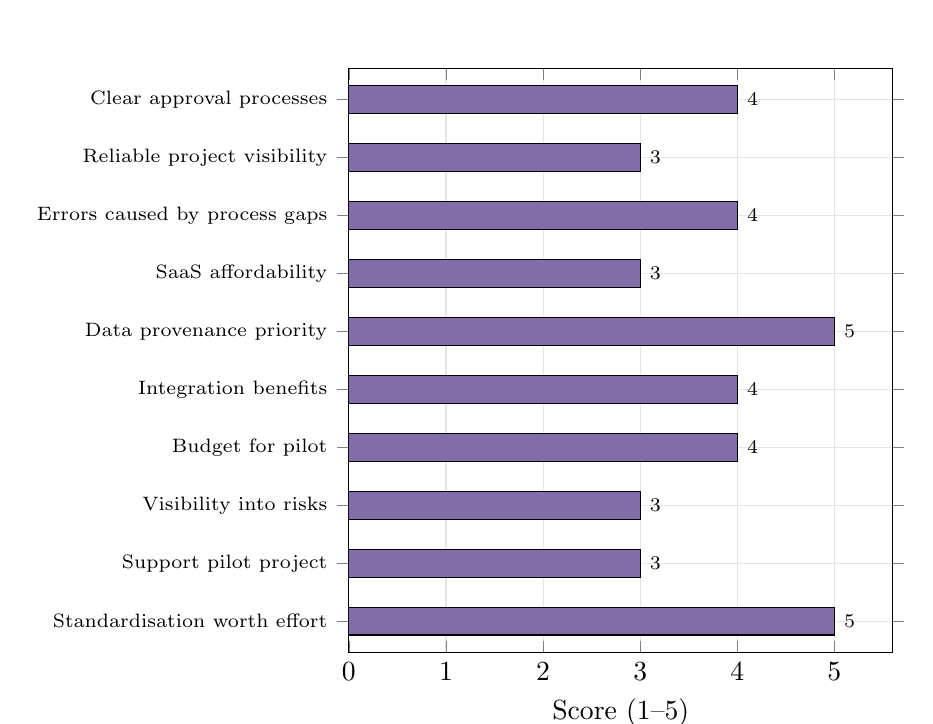
\begin{tikzpicture}
\begin{axis}[
    xbar,
    width=0.7\textwidth,
    height=9cm,
    xmin=0, xmax=5.6,
    xtick={0,1,2,3,4,5},
    xlabel={Score (1--5)},
    bar width=10pt,
    enlarge y limits=0.06,
    nodes near coords, nodes near coords align={horizontal},
    every node near coord/.append style={font=\scriptsize},
    symbolic y coords={
        {Standardisation worth effort},
        {Support pilot project},
        {Visibility into risks},
        {Budget for pilot},
        {Integration benefits},
        {Data provenance priority},
        {SaaS affordability},
        {Errors caused by process gaps},
        {Reliable project visibility},
        {Clear approval processes}
    },
    ytick=data,
    y tick label style={font=\scriptsize},
    grid=major, major grid style={draw=gray!20},
]
\addplot[fill=primary!70] coordinates {
    (4,{Clear approval processes})
    (3,{Reliable project visibility})
    (4,{Errors caused by process gaps})
    (3,{SaaS affordability})
    (5,{Data provenance priority})
    (4,{Integration benefits})
    (4,{Budget for pilot})
    (3,{Visibility into risks})
    (3,{Support pilot project})
    (5,{Standardisation worth effort})
};
\end{axis}
\end{tikzpicture}
\caption{CEO Questionnaire Results}
\label{fig:ceo_q}
\end{figure}

\textbf{Key findings:} strong support for standardisation; data governance considered critical; moderate confidence in current visibility; and strong support for integration initiatives.

% ----------------------------------------------------------------
% HR
% ----------------------------------------------------------------
\subsubsection{HR Questionnaire Results}
HR responses (Figure~\ref{fig:hr_q}) highlight weak knowledge management and cross-training, while indicating that staff are generally receptive to change.

\begin{figure}[H]
\centering
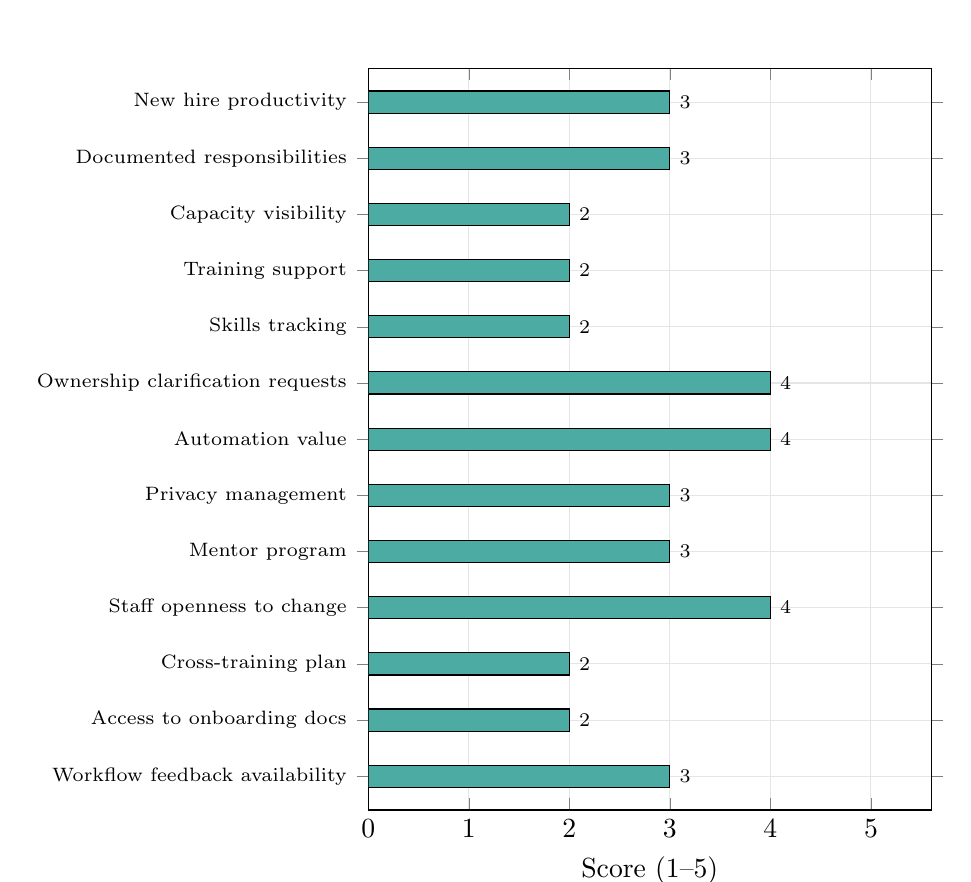
\begin{tikzpicture}
\begin{axis}[
    xbar,
    width=0.72\textwidth,
    height=11cm,
    xmin=0, xmax=5.6,
    xtick={0,1,2,3,4,5},
    xlabel={Score (1--5)},
    bar width=8pt,
    enlarge y limits=0.05,
    nodes near coords, nodes near coords align={horizontal},
    every node near coord/.append style={font=\scriptsize},
    symbolic y coords={
        {Workflow feedback availability},
        {Access to onboarding docs},
        {Cross-training plan},
        {Staff openness to change},
        {Mentor program},
        {Privacy management},
        {Automation value},
        {Ownership clarification requests},
        {Skills tracking},
        {Training support},
        {Capacity visibility},
        {Documented responsibilities},
        {New hire productivity}
    },
    ytick=data,
    y tick label style={font=\scriptsize},
    grid=major, major grid style={draw=gray!20},
]
\addplot[fill=accent!70] coordinates {
    (3,{New hire productivity})
    (3,{Documented responsibilities})
    (2,{Capacity visibility})
    (2,{Training support})
    (2,{Skills tracking})
    (4,{Ownership clarification requests})
    (4,{Automation value})
    (3,{Privacy management})
    (3,{Mentor program})
    (4,{Staff openness to change})
    (2,{Cross-training plan})
    (2,{Access to onboarding docs})
    (3,{Workflow feedback availability})
};
\end{axis}
\end{tikzpicture}
\caption{HR Questionnaire Results}
\label{fig:hr_q}
\end{figure}

\textbf{Key findings:} weak knowledge management; weak cross-training; staff generally receptive to change; and frequent ownership confusion.

% ----------------------------------------------------------------
% Engineering Manager
% ----------------------------------------------------------------
\subsubsection{Engineering Manager Questionnaire Results}
The Engineering Manager's day-to-day operational view (Figure~\ref{fig:em_q}) provides strong evidence of tool fragmentation and low confidence in documentation access, alongside strong support for workflow automation.

\begin{figure}[H]
\centering
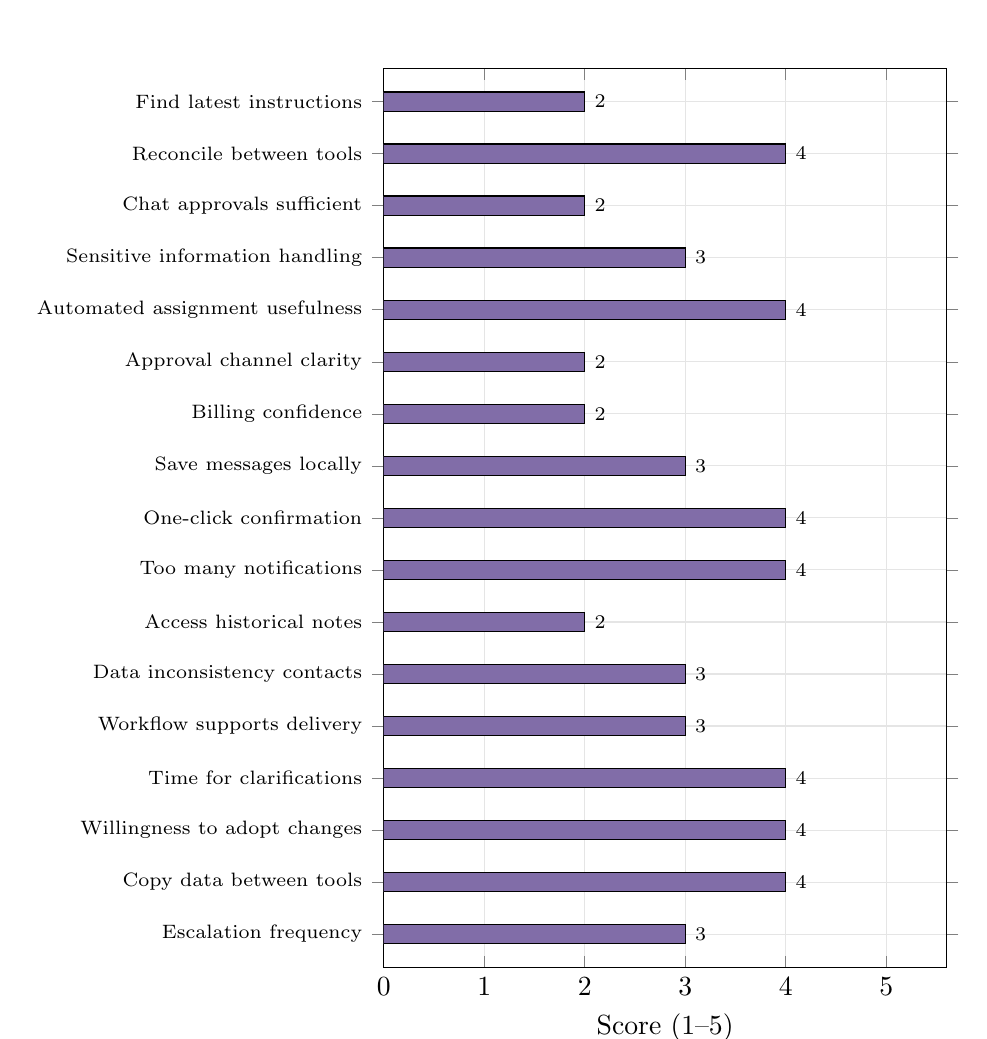
\begin{tikzpicture}
\begin{axis}[
    xbar,
    width=0.72\textwidth,
    height=13cm,
    xmin=0, xmax=5.6,
    xtick={0,1,2,3,4,5},
    xlabel={Score (1--5)},
    bar width=7pt,
    enlarge y limits=0.04,
    nodes near coords, nodes near coords align={horizontal},
    every node near coord/.append style={font=\scriptsize},
    symbolic y coords={
        {Escalation frequency},
        {Copy data between tools},
        {Willingness to adopt changes},
        {Time for clarifications},
        {Workflow supports delivery},
        {Data inconsistency contacts},
        {Access historical notes},
        {Too many notifications},
        {One-click confirmation},
        {Save messages locally},
        {Billing confidence},
        {Approval channel clarity},
        {Automated assignment usefulness},
        {Sensitive information handling},
        {Chat approvals sufficient},
        {Reconcile between tools},
        {Find latest instructions}
    },
    ytick=data,
    y tick label style={font=\scriptsize},
    grid=major, major grid style={draw=gray!20},
]
\addplot[fill=primary!70] coordinates {
    (2,{Find latest instructions})
    (4,{Reconcile between tools})
    (2,{Chat approvals sufficient})
    (3,{Sensitive information handling})
    (4,{Automated assignment usefulness})
    (2,{Approval channel clarity})
    (2,{Billing confidence})
    (3,{Save messages locally})
    (4,{One-click confirmation})
    (4,{Too many notifications})
    (2,{Access historical notes})
    (3,{Data inconsistency contacts})
    (3,{Workflow supports delivery})
    (4,{Time for clarifications})
    (4,{Willingness to adopt changes})
    (4,{Copy data between tools})
    (3,{Escalation frequency})
};
\end{axis}
\end{tikzpicture}
\caption{Engineering Manager Questionnaire Results}
\label{fig:em_q}
\end{figure}

\textbf{Key findings:} strong evidence of tool fragmentation; low confidence in documentation access; and strong support for workflow automation.

% ----------------------------------------------------------------
% EMPLOYEES (7 charts)
% ----------------------------------------------------------------
\subsubsection{Employee Survey Results}
The employee survey captured response distributions across fifteen Likert items and two frequency items. The following charts group related items to expose specific operational pain points, ending with a summary of average scores by problem area.

% --- Fig: Info access ---
\begin{figure}[H]
\centering
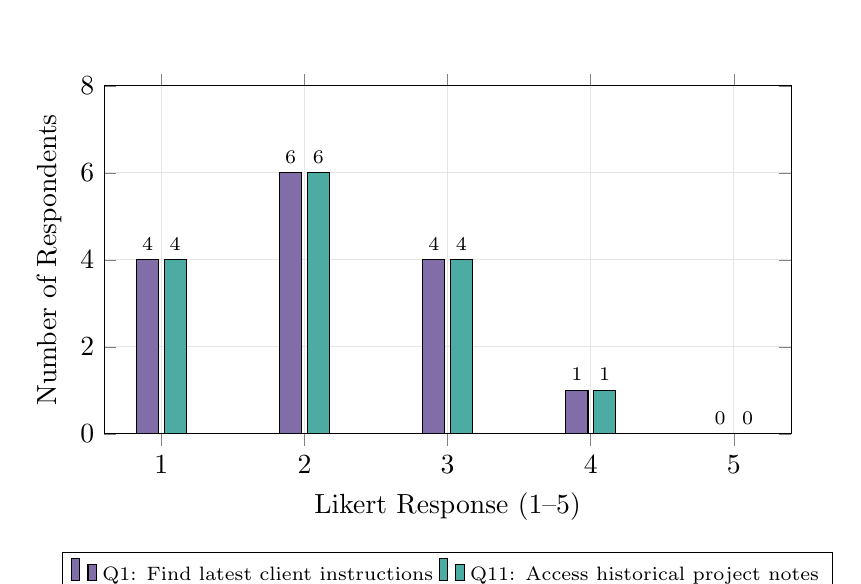
\begin{tikzpicture}
\begin{axis}[
    ybar,
    width=0.85\textwidth, height=6cm,
    bar width=8pt,
    ymin=0, ymax=8,
    ylabel={Number of Respondents},
    xlabel={Likert Response (1--5)},
    symbolic x coords={1,2,3,4,5},
    xtick=data,
    nodes near coords, every node near coord/.append style={font=\scriptsize},
    legend style={at={(0.5,-0.34)}, anchor=north, legend columns=2, font=\scriptsize},
    grid=major, major grid style={draw=gray!20},
]
\addplot[fill=primary!70] coordinates {(1,4)(2,6)(3,4)(4,1)(5,0)};
\addplot[fill=accent!70]  coordinates {(1,4)(2,6)(3,4)(4,1)(5,0)};
\legend{Q1: Find latest client instructions, Q11: Access historical project notes}
\end{axis}
\end{tikzpicture}
\caption{Employee Difficulty Finding and Accessing Project Information}
\label{fig:emp_info}
\end{figure}
\textbf{Supports:} fragmented communication and lack of knowledge management. Most employees disagree that they can readily locate current instructions or historical notes.

% --- Fig: Fragmentation ---
\begin{figure}[H]
\centering
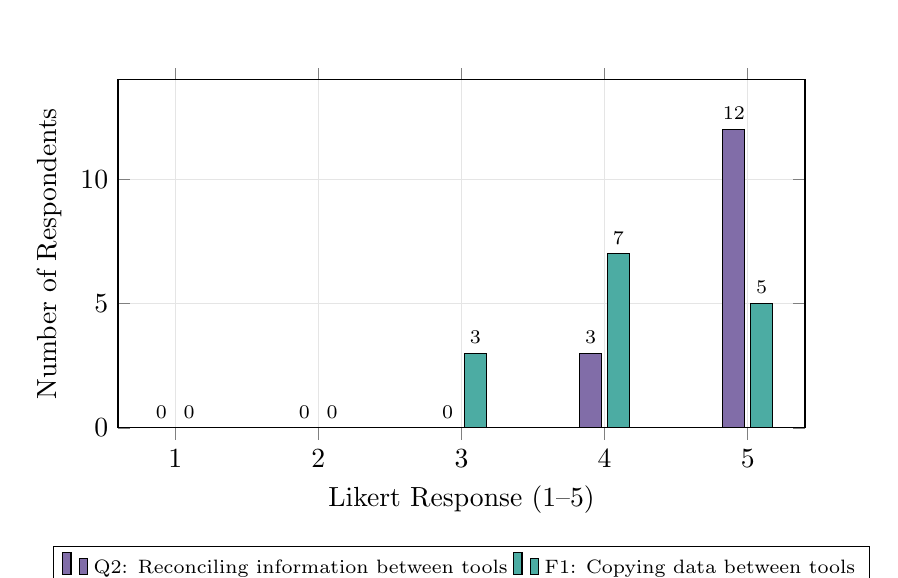
\begin{tikzpicture}
\begin{axis}[
    ybar,
    width=0.85\textwidth, height=6cm,
    bar width=8pt,
    ymin=0, ymax=14,
    ylabel={Number of Respondents},
    xlabel={Likert Response (1--5)},
    symbolic x coords={1,2,3,4,5},
    xtick=data,
    nodes near coords, every node near coord/.append style={font=\scriptsize},
    legend style={at={(0.5,-0.34)}, anchor=north, legend columns=2, font=\scriptsize},
    grid=major, major grid style={draw=gray!20},
]
\addplot[fill=primary!70] coordinates {(1,0)(2,0)(3,0)(4,3)(5,12)};
\addplot[fill=accent!70]  coordinates {(1,0)(2,0)(3,3)(4,7)(5,5)};
\legend{Q2: Reconciling information between tools, F1: Copying data between tools}
\end{axis}
\end{tikzpicture}
\caption{Employee-Reported Impact of System Fragmentation}
\label{fig:emp_frag}
\end{figure}
\textbf{Supports:} system fragmentation and manual processes. This is among the strongest signals in the survey --- the overwhelming majority of employees frequently reconcile and copy data between tools.

% --- Fig: Approvals ---
\begin{figure}[H]
\centering
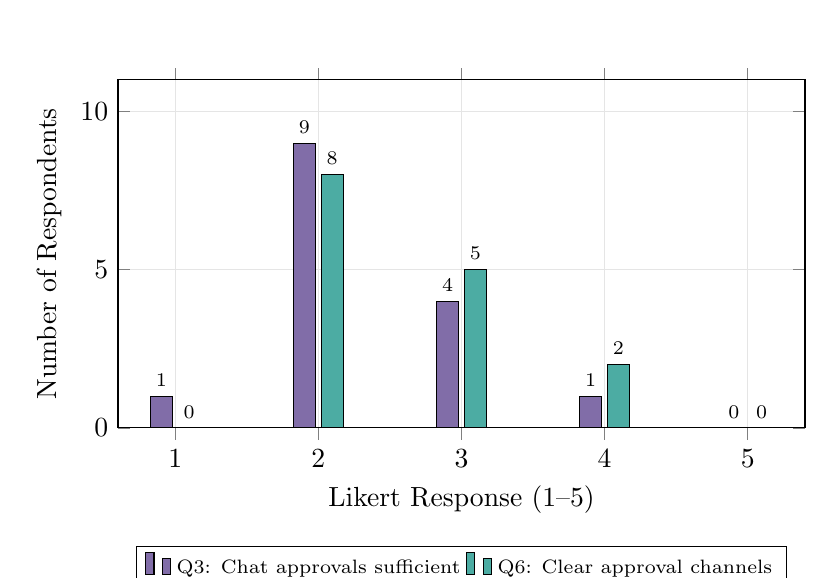
\begin{tikzpicture}
\begin{axis}[
    ybar,
    width=0.85\textwidth, height=6cm,
    bar width=8pt,
    ymin=0, ymax=11,
    ylabel={Number of Respondents},
    xlabel={Likert Response (1--5)},
    symbolic x coords={1,2,3,4,5},
    xtick=data,
    nodes near coords, every node near coord/.append style={font=\scriptsize},
    legend style={at={(0.5,-0.34)}, anchor=north, legend columns=2, font=\scriptsize},
    grid=major, major grid style={draw=gray!20},
]
\addplot[fill=primary!70] coordinates {(1,1)(2,9)(3,4)(4,1)(5,0)};
\addplot[fill=accent!70]  coordinates {(1,0)(2,8)(3,5)(4,2)(5,0)};
\legend{Q3: Chat approvals sufficient, Q6: Clear approval channels}
\end{axis}
\end{tikzpicture}
\caption{Employee Approval and Communication Challenges}
\label{fig:emp_appr}
\end{figure}
\textbf{Supports:} WhatsApp dependency and an informal approval process. Few employees consider chat approvals sufficient or feel they have clear approval channels.

% --- Fig: Governance ---
\begin{figure}[H]
\centering
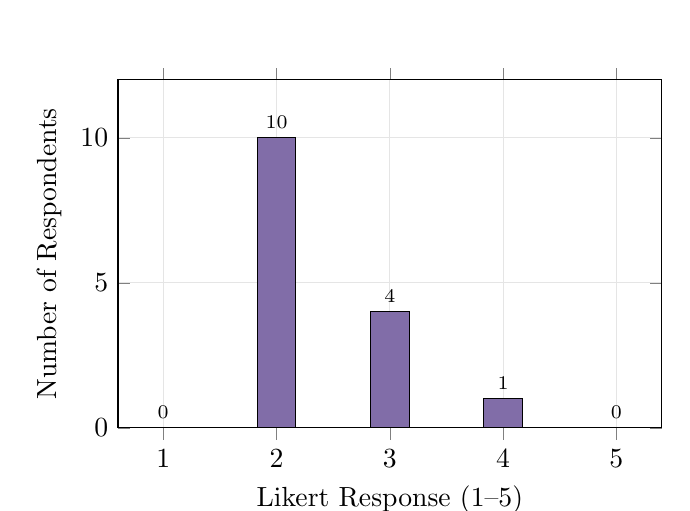
\begin{tikzpicture}
\begin{axis}[
    ybar,
    width=0.7\textwidth, height=6cm,
    bar width=14pt,
    ymin=0, ymax=12,
    ylabel={Number of Respondents},
    xlabel={Likert Response (1--5)},
    symbolic x coords={1,2,3,4,5},
    xtick=data,
    nodes near coords, every node near coord/.append style={font=\scriptsize},
    grid=major, major grid style={draw=gray!20},
]
\addplot[fill=primary!70] coordinates {(1,0)(2,10)(3,4)(4,1)(5,0)};
\end{axis}
\end{tikzpicture}
\caption{Employee Confidence in Billing Record Accuracy (Q7)}
\label{fig:emp_gov}
\end{figure}
\textbf{Supports:} data governance issues and multiple sources of truth. Confidence in billing-record accuracy is low, concentrated at the disagree end of the scale.

% --- Fig: Security ---
\begin{figure}[H]
\centering
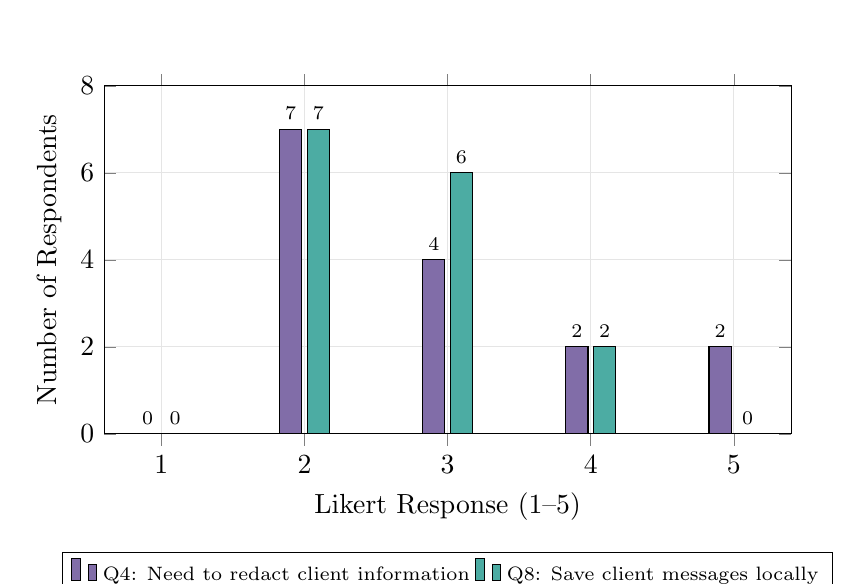
\begin{tikzpicture}
\begin{axis}[
    ybar,
    width=0.85\textwidth, height=6cm,
    bar width=8pt,
    ymin=0, ymax=8,
    ylabel={Number of Respondents},
    xlabel={Likert Response (1--5)},
    symbolic x coords={1,2,3,4,5},
    xtick=data,
    nodes near coords, every node near coord/.append style={font=\scriptsize},
    legend style={at={(0.5,-0.34)}, anchor=north, legend columns=2, font=\scriptsize},
    grid=major, major grid style={draw=gray!20},
]
\addplot[fill=primary!70] coordinates {(1,0)(2,7)(3,4)(4,2)(5,2)};
\addplot[fill=accent!70]  coordinates {(1,0)(2,7)(3,6)(4,2)(5,0)};
\legend{Q4: Need to redact client information, Q8: Save client messages locally}
\end{axis}
\end{tikzpicture}
\caption{Employee Security and Sensitive Information Handling}
\label{fig:emp_sec}
\end{figure}
\textbf{Supports:} security risks and informal data handling. A notable share of employees report needing to redact client information and saving client messages locally.

% --- Fig: Automation readiness ---
\begin{figure}[H]
\centering
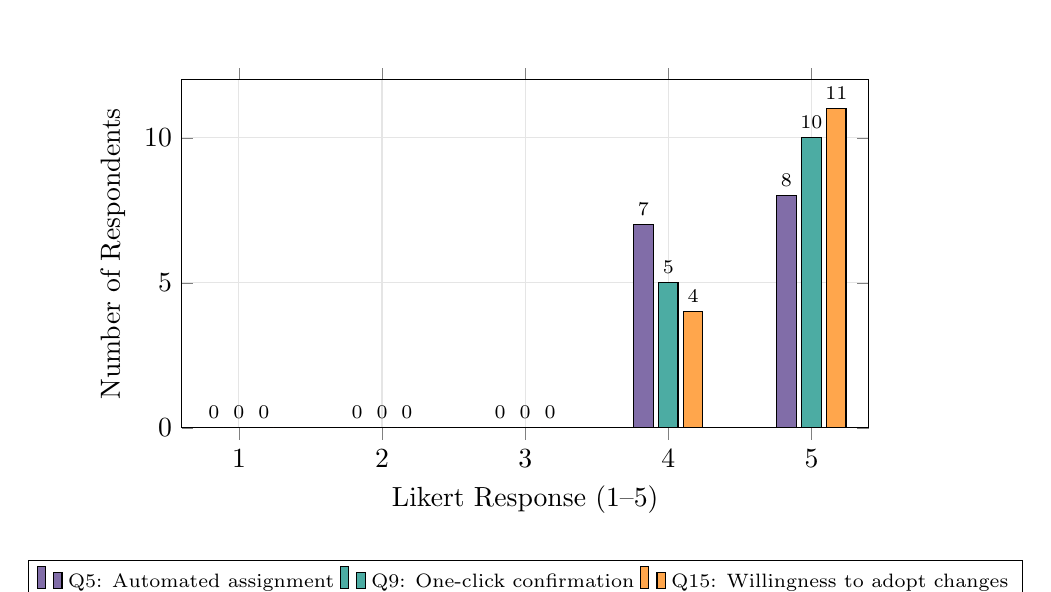
\begin{tikzpicture}
\begin{axis}[
    ybar,
    width=0.85\textwidth, height=6cm,
    bar width=7pt,
    ymin=0, ymax=12,
    ylabel={Number of Respondents},
    xlabel={Likert Response (1--5)},
    symbolic x coords={1,2,3,4,5},
    xtick=data,
    nodes near coords, every node near coord/.append style={font=\scriptsize},
    legend style={at={(0.5,-0.38)}, anchor=north, legend columns=3, font=\scriptsize},
    grid=major, major grid style={draw=gray!20},
]
\addplot[fill=primary!70] coordinates {(1,0)(2,0)(3,0)(4,7)(5,8)};
\addplot[fill=accent!70]  coordinates {(1,0)(2,0)(3,0)(4,5)(5,10)};
\addplot[fill=orange!70]  coordinates {(1,0)(2,0)(3,0)(4,4)(5,11)};
\legend{Q5: Automated assignment, Q9: One-click confirmation, Q15: Willingness to adopt changes}
\end{axis}
\end{tikzpicture}
\caption{Employee Readiness for Process Automation}
\label{fig:emp_auto}
\end{figure}
\textbf{Supports:} scalability issues and the feasibility of the proposed system. Every employee response falls at ``agree'' or ``strongly agree'', justifying the proposed automation later in the report.

% --- Fig: Average by problem area ---
\begin{figure}[H]
\centering
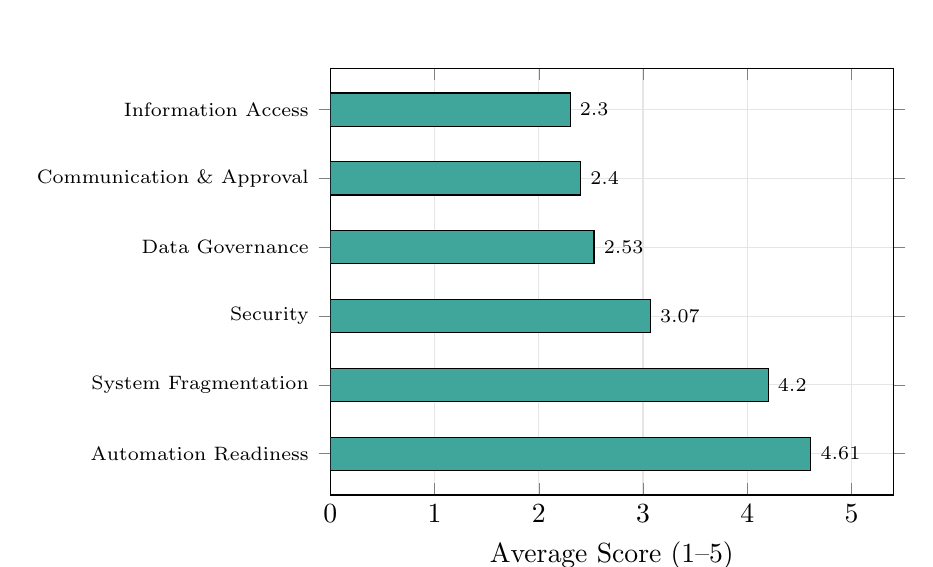
\begin{tikzpicture}
\begin{axis}[
    xbar,
    width=0.72\textwidth, height=7cm,
    xmin=0, xmax=5.4,
    xtick={0,1,2,3,4,5},
    xlabel={Average Score (1--5)},
    bar width=12pt,
    enlarge y limits=0.12,
    nodes near coords, nodes near coords align={horizontal},
    every node near coord/.append style={font=\scriptsize},
    symbolic y coords={
        {Automation Readiness},
        {System Fragmentation},
        {Security},
        {Data Governance},
        {Communication \& Approval},
        {Information Access}
    },
    ytick=data,
    y tick label style={font=\scriptsize},
    grid=major, major grid style={draw=gray!20},
]
\addplot[fill=accent!75] coordinates {
    (2.30,{Information Access})
    (2.40,{Communication \& Approval})
    (2.53,{Data Governance})
    (3.07,{Security})
    (4.20,{System Fragmentation})
    (4.61,{Automation Readiness})
};
\end{axis}
\end{tikzpicture}
\caption{Average Employee Score by Problem Area}
\label{fig:emp_avg}
\end{figure}
\textbf{Summary chart.} This view clearly shows that (1) system fragmentation is the biggest pain point, (2) employees strongly support automation, (3) information access and communication are weak, and (4) security is moderate but still concerning.

% ----------------------------------------------------------------
% CUSTOMERS
% ----------------------------------------------------------------
\subsubsection{Customer Questionnaire Results}
Customer responses (Figure~\ref{fig:cust_q}) indicate generally positive satisfaction, with a clear preference for more formal approval mechanisms.

\begin{figure}[H]
\centering
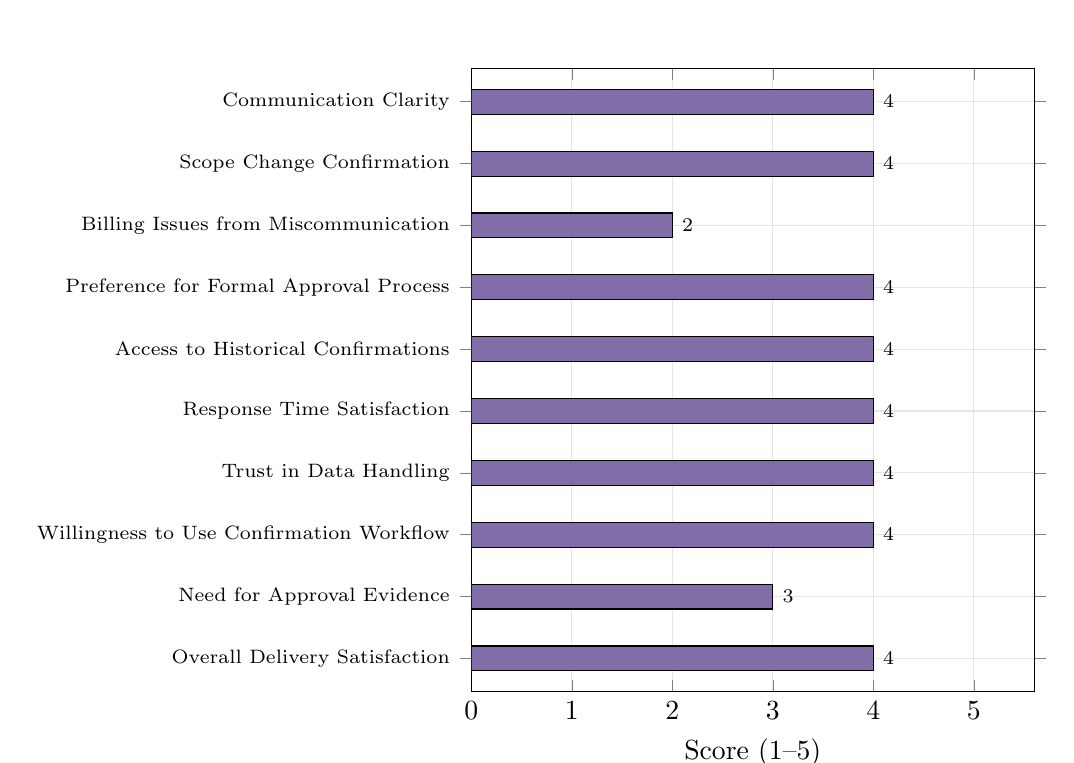
\begin{tikzpicture}
\begin{axis}[
    xbar,
    width=0.72\textwidth, height=9.5cm,
    xmin=0, xmax=5.6,
    xtick={0,1,2,3,4,5},
    xlabel={Score (1--5)},
    bar width=9pt,
    enlarge y limits=0.06,
    nodes near coords, nodes near coords align={horizontal},
    every node near coord/.append style={font=\scriptsize},
    symbolic y coords={
        {Overall Delivery Satisfaction},
        {Need for Approval Evidence},
        {Willingness to Use Confirmation Workflow},
        {Trust in Data Handling},
        {Response Time Satisfaction},
        {Access to Historical Confirmations},
        {Preference for Formal Approval Process},
        {Billing Issues from Miscommunication},
        {Scope Change Confirmation},
        {Communication Clarity}
    },
    ytick=data,
    y tick label style={font=\scriptsize},
    grid=major, major grid style={draw=gray!20},
]
\addplot[fill=primary!70] coordinates {
    (4,{Communication Clarity})
    (4,{Scope Change Confirmation})
    (2,{Billing Issues from Miscommunication})
    (4,{Preference for Formal Approval Process})
    (4,{Access to Historical Confirmations})
    (4,{Response Time Satisfaction})
    (4,{Trust in Data Handling})
    (4,{Willingness to Use Confirmation Workflow})
    (3,{Need for Approval Evidence})
    (4,{Overall Delivery Satisfaction})
};
\end{axis}
\end{tikzpicture}
\caption{Customer Questionnaire Results}
\label{fig:cust_q}
\end{figure}

The customer questionnaire indicates generally positive satisfaction with project delivery, communication quality, response times, and data handling practices. However, customers expressed a preference for more formal approval mechanisms and indicated occasional needs for documented approval evidence during billing and audit activities. These findings support the proposed introduction of structured approval workflows and centralised record management, while suggesting that the operational issues identified internally have not yet significantly affected overall customer satisfaction.

% ----------------------------------------------------------------
% COMPARISON CHARTS
% ----------------------------------------------------------------
\subsubsection{Stakeholder Comparison of Key Issues}
Mapping a few representative questions to the identified problems shows that different stakeholder groups perceive the same underlying issues (Figure~\ref{fig:stake_cmp}).

\begin{figure}[H]
\centering
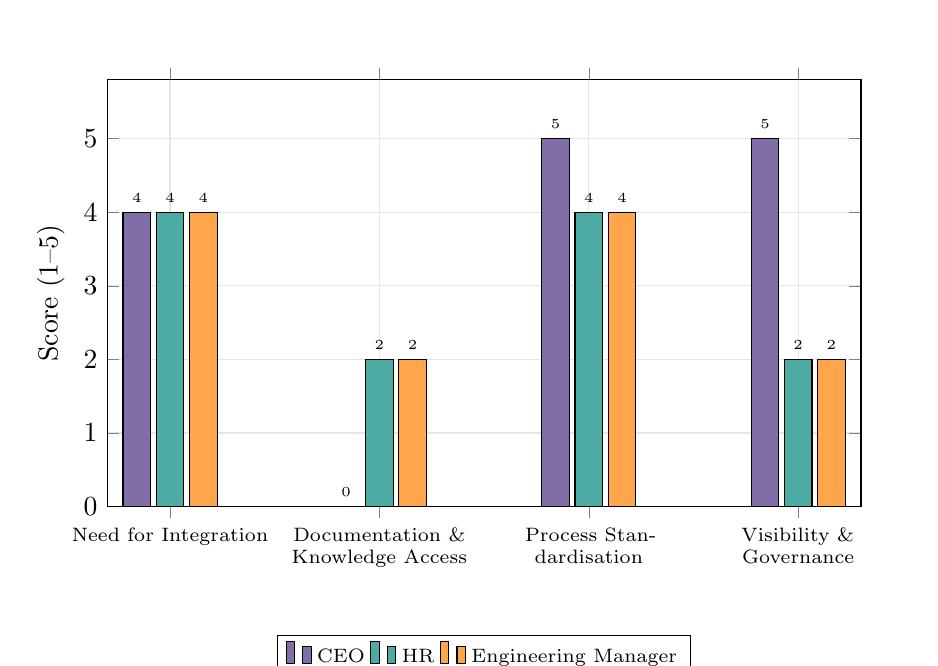
\begin{tikzpicture}
\begin{axis}[
    ybar,
    width=0.92\textwidth, height=7cm,
    bar width=10pt,
    ymin=0, ymax=5.8,
    ytick={0,1,2,3,4,5},
    ylabel={Score (1--5)},
    symbolic x coords={
        {Need for Integration},
        {Documentation \& Knowledge Access},
        {Process Standardisation},
        {Visibility \& Governance}
    },
    xtick=data,
    x tick label style={font=\scriptsize, text width=2.6cm, align=center},
    nodes near coords, every node near coord/.append style={font=\tiny},
    legend style={at={(0.5,-0.30)}, anchor=north, legend columns=3, font=\scriptsize},
    grid=major, major grid style={draw=gray!20},
]
\addplot[fill=primary!70] coordinates {
    ({Need for Integration},4) ({Documentation \& Knowledge Access},0)
    ({Process Standardisation},5) ({Visibility \& Governance},5)};
\addplot[fill=accent!70] coordinates {
    ({Need for Integration},4) ({Documentation \& Knowledge Access},2)
    ({Process Standardisation},4) ({Visibility \& Governance},2)};
\addplot[fill=orange!70] coordinates {
    ({Need for Integration},4) ({Documentation \& Knowledge Access},2)
    ({Process Standardisation},4) ({Visibility \& Governance},2)};
\legend{CEO, HR, Engineering Manager}
\end{axis}
\end{tikzpicture}
\caption{Stakeholder Comparison of Key Issues}
\label{fig:stake_cmp}
\end{figure}

\textbf{Note:} the CEO did not respond to the documentation/knowledge-access item, shown here as zero. This comparison demonstrates that leadership prioritises governance, HR emphasises workforce readiness, and the Engineering Manager experiences operational inefficiencies directly --- yet all groups support process improvement.

\subsubsection{Stakeholder Support for Process Standardisation and Automation}
Finally, aggregating each group's support for standardisation and workflow improvement (Figure~\ref{fig:stake_support}) shows broad, cross-cutting endorsement of change.

\begin{figure}[H]
\centering
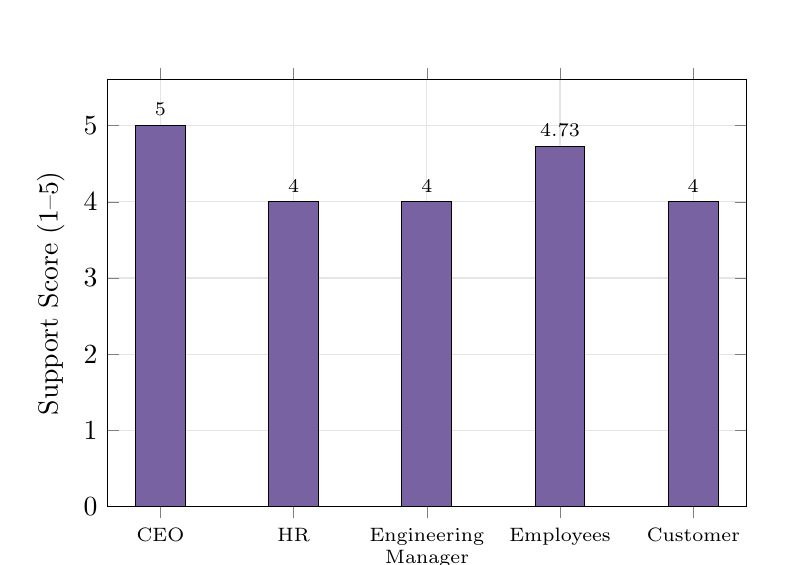
\begin{tikzpicture}
\begin{axis}[
    ybar,
    width=0.8\textwidth, height=7cm,
    bar width=18pt,
    ymin=0, ymax=5.6,
    ytick={0,1,2,3,4,5},
    ylabel={Support Score (1--5)},
    symbolic x coords={CEO, HR, {Engineering Manager}, Employees, Customer},
    xtick=data,
    x tick label style={font=\scriptsize, text width=2cm, align=center},
    nodes near coords, every node near coord/.append style={font=\scriptsize},
    grid=major, major grid style={draw=gray!20},
]
\addplot[fill=primary!75] coordinates {
    (CEO,5) (HR,4) ({Engineering Manager},4) (Employees,4.73) (Customer,4)};
\end{axis}
\end{tikzpicture}
\caption{Stakeholder Support for Process Standardisation and Workflow Improvements}
\label{fig:stake_support}
\end{figure}

This final chart captures the central conclusion of the analysis: the proposed information-system improvements are supported by all major stakeholder groups --- leadership, management, employees, and customers alike. That consensus provides a strong mandate for the system design work that follows in the next chapter.

% ================================================================
% REPLACEMENT SECTION: Data Flow Diagrams (5 Level-1 DFDs, one per problem)
% This replaces the old "4.3.2.2 Subsystem DFDs" part.
% Keep the Context Diagram (Level 0) as-is, then add five focused Level-1 DFDs.
% ================================================================

\subsection{Data Flow Diagram (DFD) of Existing System}

Data Flow Diagrams (DFDs) were developed to represent the flow of information within NextStepBD's current operational environment. The diagrams illustrate how information is created, transferred, stored, and utilised across different stakeholders and systems. The purpose of these DFDs is to identify inefficiencies, duplication of effort, communication gaps, and operational bottlenecks within the existing environment.

The analysis revealed that information frequently moves through multiple disconnected platforms including WhatsApp, Email, Google Sheets, GitHub, and manual records. As a result, critical business information is often duplicated, inconsistently maintained, and difficult to trace. The DFDs presented below visualise these issues and provide the foundation for the improved system proposed in later chapters.

The diagrams use standard DFD notation: \emph{external entities} are shown as solid rectangles, \emph{processes} as circles, \emph{data stores} as open-ended (Gane--Sarson style) bars, and \emph{data flows} as labelled directed arrows.

% ----------------------------------------------------------------
% 4.3.2.1 Context Diagram (Level 0) — kept unchanged
% ----------------------------------------------------------------
\subsubsection{DFD of Whole Existing System (Context Diagram)}

The Context DFD (Figure~\ref{fig:dfd_context}) provides a high-level view of the entire organisation as a single system (\textbf{P0}) and illustrates its interactions with four external entities: Customers (E1), Management/CEO (E2), Employees (E3), and the HR Department (E4). Process P0 represents all operational activities currently performed by the company using a combination of manual procedures and disconnected software tools.

\begin{figure}[H]
\centering
\resizebox{0.92\textwidth}{!}{
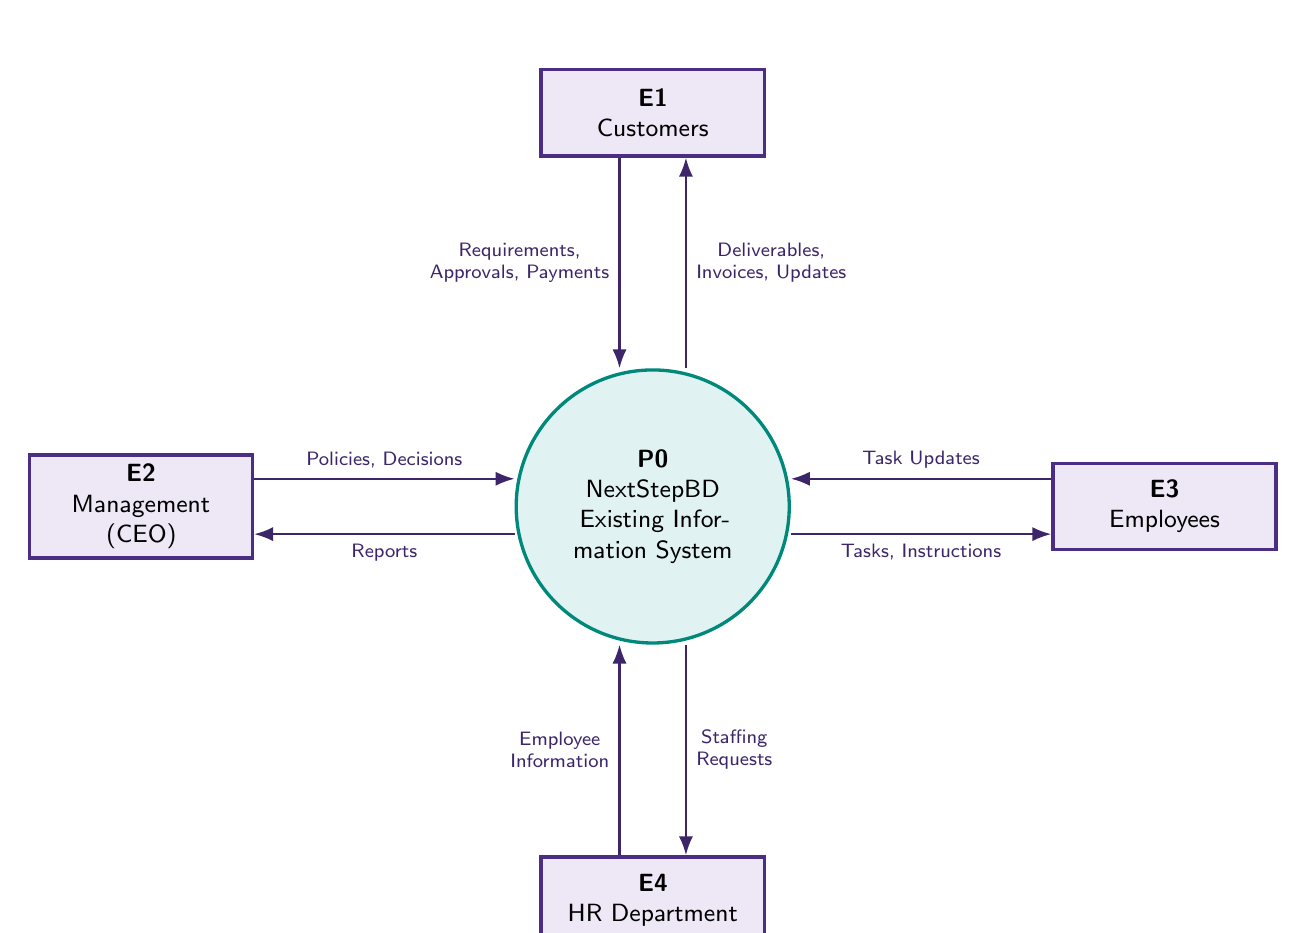
\begin{tikzpicture}[
    every node/.style={font=\sffamily\small},
    entity/.style={rectangle, draw=primary, fill=secondary, very thick, text width=2.6cm, align=center, minimum height=1.1cm},
    proc/.style={circle, draw=accent, fill=softteal, very thick, text width=2.8cm, align=center, minimum size=3.2cm},
    flow/.style={-{Latex[length=2.4mm]}, thick, color=primary!80!black},
    flab/.style={font=\scriptsize\sffamily, align=center}
]
% Central process
\node[proc] (p0) at (0,0) {\textbf{P0}\\NextStepBD Existing Information System};

% External entities (corners)
\node[entity] (cust) at (0,5)    {\textbf{E1}\\Customers};
\node[entity] (ceo)  at (-6.5,0) {\textbf{E2}\\Management (CEO)};
\node[entity] (emp)  at (6.5,0)  {\textbf{E3}\\Employees};
\node[entity] (hr)   at (0,-5)   {\textbf{E4}\\HR Department};

% Customer flows
\draw[flow] ([xshift=-12pt]cust.south) -- ([xshift=-12pt]p0.north)
    node[flab, midway, left] {Requirements,\\Approvals, Payments};
\draw[flow] ([xshift=12pt]p0.north) -- ([xshift=12pt]cust.south)
    node[flab, midway, right] {Deliverables,\\Invoices, Updates};

% CEO flows
\draw[flow] ([yshift=10pt]ceo.east) -- ([yshift=10pt]p0.west)
    node[flab, midway, above] {Policies, Decisions};
\draw[flow] ([yshift=-10pt]p0.west) -- ([yshift=-10pt]ceo.east)
    node[flab, midway, below] {Reports};

% Employees flows
\draw[flow] ([yshift=10pt]emp.west) -- ([yshift=10pt]p0.east)
    node[flab, midway, above] {Task Updates};
\draw[flow] ([yshift=-10pt]p0.east) -- ([yshift=-10pt]emp.west)
    node[flab, midway, below] {Tasks, Instructions};

% HR flows
\draw[flow] ([xshift=-12pt]hr.north) -- ([xshift=-12pt]p0.south)
    node[flab, midway, left] {Employee\\Information};
\draw[flow] ([xshift=12pt]p0.south) -- ([xshift=12pt]hr.north)
    node[flab, midway, right] {Staffing\\Requests};
\end{tikzpicture}
}
\caption{Context Diagram (Level 0) of the Existing Information System}
\label{fig:dfd_context}
\end{figure}

\noindent The context diagram makes clear that every external entity transacts through a single, undifferentiated information ``system'' that is in reality a patchwork of manual procedures and disconnected tools. This single point of mediation is where most of the company's traceability and reconciliation problems originate.

% ----------------------------------------------------------------
% NEW: Five separate Level-1 DFDs — one for each identified problem
% ----------------------------------------------------------------
\subsubsection{Level 1 DFDs — One per Identified Problem Area}

The following five Level~1 DFDs provide focused views of the current system, each centred on one of the five priority problems identified in Chapter~1. Each diagram highlights the specific processes, data stores, and flows that contribute to that problem.

% ========================================================
% PROBLEM 1: Fragmented Communication & Collaboration
% ========================================================
\paragraph{A. Level 1 DFD — Problem 1: Fragmented Communication \& Collaboration}

This diagram (Figure~\ref{fig:dfd_prob1}) focuses on how requirements, approvals, and decisions flow through informal channels. It shows the heavy reliance on WhatsApp and email as both communication medium and de-facto record, with almost no structured capture into project artefacts.

\begin{figure}[H]
\centering
\resizebox{\textwidth}{!}{
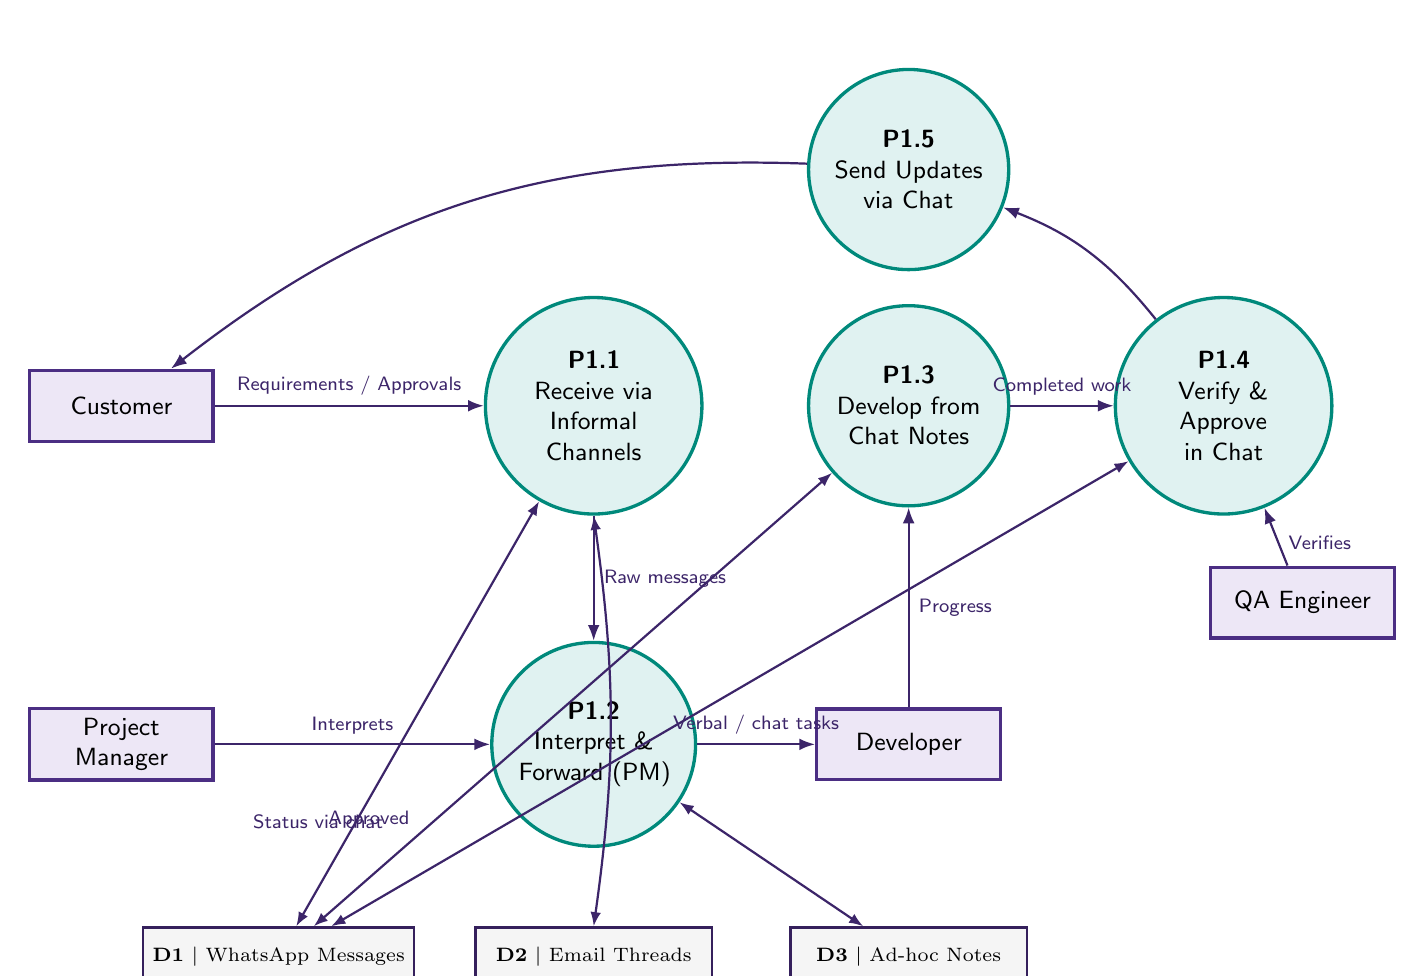
\begin{tikzpicture}[
    every node/.style={font=\sffamily\small},
    entity/.style={rectangle, draw=primary, fill=secondary, very thick, text width=2.1cm, align=center, minimum height=0.9cm},
    proc/.style={circle, draw=accent, fill=softteal, very thick, text width=2.0cm, align=center, minimum size=2.4cm},
    flow/.style={-{Latex[length=2.0mm]}, thick, color=primary!80!black},
    store/.style={thick, color=primary!70!black},
    flab/.style={font=\scriptsize\sffamily, align=center}
]
% External entities
\node[entity] (cust) at (-2.5,5.5) {Customer};
\node[entity] (pm)   at (-2.5,1.2) {Project Manager};
\node[entity] (dev)  at (7.5,1.2)  {Developer};
\node[entity] (qa)   at (12.5,3.0) {QA Engineer};

% Processes (Problem 1 focus)
\node[proc] (p11) at (3.5,5.5)  {\textbf{P1.1}\\Receive via\\Informal Channels};
\node[proc] (p12) at (3.5,1.2)  {\textbf{P1.2}\\Interpret \&\\Forward (PM)};
\node[proc] (p13) at (7.5,5.5)  {\textbf{P1.3}\\Develop from\\Chat Notes};
\node[proc] (p14) at (11.5,5.5) {\textbf{P1.4}\\Verify \&\\Approve in Chat};
\node[proc] (p15) at (7.5,8.5)  {\textbf{P1.5}\\Send Updates\\via Chat};

% Problematic data stores
\node[draw=primary!70!black, fill=softgray, thick, minimum width=3.2cm, minimum height=0.75cm, align=center, font=\scriptsize] (d1) at (-0.5,-1.5) {\textbf{D1} \textbar{} WhatsApp Messages};
\node[draw=primary!70!black, fill=softgray, thick, minimum width=3.0cm, minimum height=0.75cm, align=center, font=\scriptsize] (d2) at (3.5,-1.5) {\textbf{D2} \textbar{} Email Threads};
\node[draw=primary!70!black, fill=softgray, thick, minimum width=3.0cm, minimum height=0.75cm, align=center, font=\scriptsize] (d3) at (7.5,-1.5) {\textbf{D3} \textbar{} Ad-hoc Notes};

% Flows
\draw[flow] (cust) -- (p11) node[flab,midway,above]{Requirements / Approvals};
\draw[flow] (pm) -- (p12) node[flab,midway,above]{Interprets};
\draw[flow] (p11) -- (p12) node[flab,midway,right]{Raw messages};
\draw[flow] (p12) -- (dev) node[flab,midway,above]{Verbal / chat tasks};
\draw[flow] (dev) -- (p13) node[flab,midway,right]{Progress};
\draw[flow] (p13) -- (p14) node[flab,midway,above]{Completed work};
\draw[flow] (qa) -- (p14) node[flab,pos=0.4,right]{Verifies};
\draw[flow] (p14) to[bend right=15] (p15) node[flab,pos=0.5,above right]{Approved};
\draw[flow] (p15) to[bend right=20] (cust) node[flab,midway,above]{Status via chat};

% Bidirectional store links (the core problem)
\draw[flow,{Latex[length=1.8mm]}-{Latex[length=1.8mm]}] (p11) -- (d1);
\draw[flow,{Latex[length=1.8mm]}-{Latex[length=1.8mm]}] (p11.south) to[bend left=8] (d2.north);
\draw[flow,{Latex[length=1.8mm]}-{Latex[length=1.8mm]}] (p12) -- (d3);
\draw[flow,{Latex[length=1.8mm]}-{Latex[length=1.8mm]}] (p13) -- (d1);
\draw[flow,{Latex[length=1.8mm]}-{Latex[length=1.8mm]}] (p14) -- (d1);
\end{tikzpicture}
}
\caption{Level~1 DFD — Problem 1: Fragmented Communication \& Collaboration}
\label{fig:dfd_prob1}
\end{figure}

\begin{problemBox}
\textbf{Key problems visible:} All approvals and decisions live only in transient chat/email stores (D1–D3). There is no structured hand-off to a canonical project record. The Project Manager is the sole interpreter and gatekeeper, creating a severe bottleneck and zero traceability.
\end{problemBox}

% ========================================================
% PROBLEM 2: System Fragmentation & Lack of Integration
% ========================================================
\paragraph{B. Level 1 DFD — Problem 2: System Fragmentation \& Lack of Integration}

This diagram (Figure~\ref{fig:dfd_prob2}) shows how the same business information is scattered across five completely separate tools with no automated synchronisation. Every cross-tool action requires manual copy-paste or re-entry.

\begin{figure}[H]
\centering
\resizebox{\textwidth}{!}{
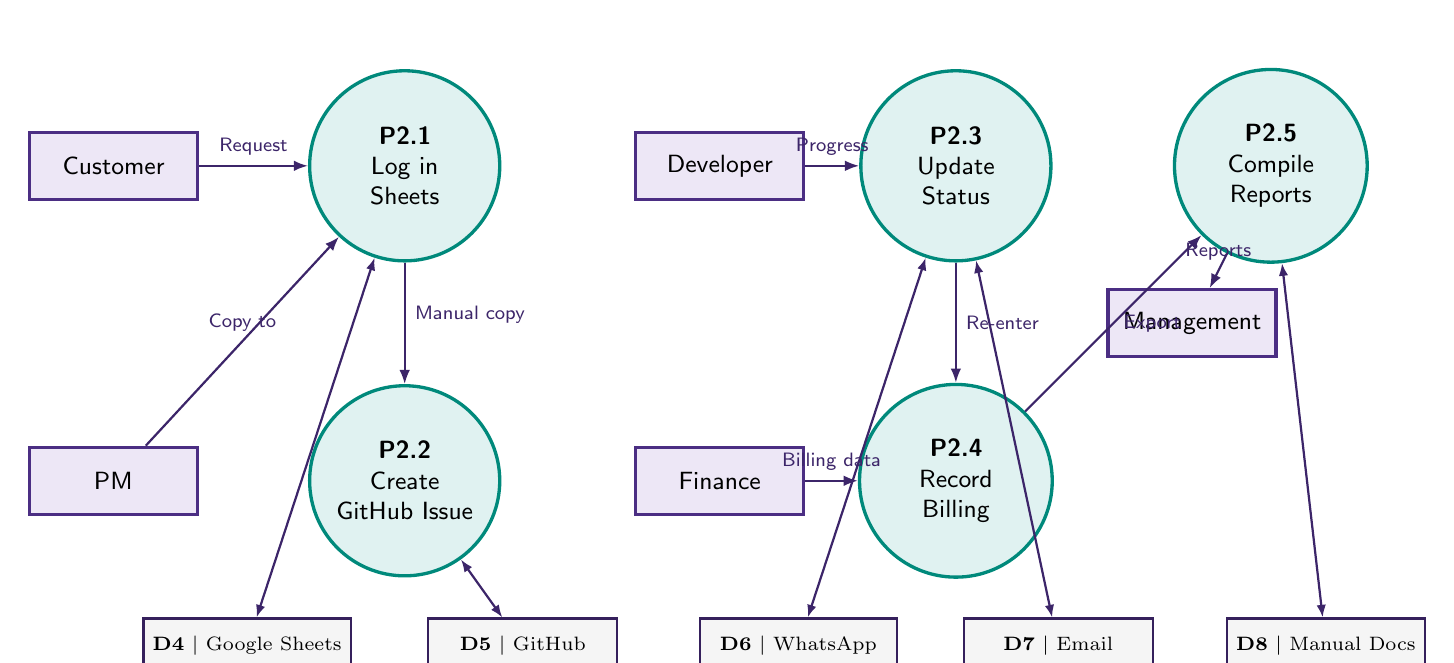
\begin{tikzpicture}[
    every node/.style={font=\sffamily\small},
    entity/.style={rectangle, draw=primary, fill=secondary, very thick, text width=1.9cm, align=center, minimum height=0.85cm},
    proc/.style={circle, draw=accent, fill=softteal, very thick, text width=1.85cm, align=center, minimum size=2.1cm},
    flow/.style={-{Latex[length=1.8mm]}, thick, color=primary!80!black},
    store/.style={thick, color=primary!70!black},
    flab/.style={font=\scriptsize\sffamily, align=center}
]
% Entities
\node[entity] (cust) at (-3.2,4.8) {Customer};
\node[entity] (pm)   at (-3.2,0.8) {PM};
\node[entity] (dev)  at (4.5,4.8)  {Developer};
\node[entity] (fin)  at (4.5,0.8)  {Finance};
\node[entity] (mgt)  at (10.5,2.8){Management};

% Processes
\node[proc] (p21) at (0.5,4.8)  {\textbf{P2.1}\\Log in\\Sheets};
\node[proc] (p22) at (0.5,0.8)  {\textbf{P2.2}\\Create\\GitHub Issue};
\node[proc] (p23) at (7.5,4.8)  {\textbf{P2.3}\\Update\\Status};
\node[proc] (p24) at (7.5,0.8)  {\textbf{P2.4}\\Record\\Billing};
\node[proc] (p25) at (11.5,4.8) {\textbf{P2.5}\\Compile\\Reports};

% Five disconnected stores (the fragmentation problem)
\node[draw=primary!70!black, fill=softgray, thick, minimum width=2.6cm, minimum height=0.7cm, align=center, font=\scriptsize] (d4) at (-1.5,-1.3) {\textbf{D4} \textbar{} Google Sheets};
\node[draw=primary!70!black, fill=softgray, thick, minimum width=2.4cm, minimum height=0.7cm, align=center, font=\scriptsize] (d5) at (2.0,-1.3) {\textbf{D5} \textbar{} GitHub};
\node[draw=primary!70!black, fill=softgray, thick, minimum width=2.5cm, minimum height=0.7cm, align=center, font=\scriptsize] (d6) at (5.5,-1.3) {\textbf{D6} \textbar{} WhatsApp};
\node[draw=primary!70!black, fill=softgray, thick, minimum width=2.4cm, minimum height=0.7cm, align=center, font=\scriptsize] (d7) at (8.8,-1.3) {\textbf{D7} \textbar{} Email};
\node[draw=primary!70!black, fill=softgray, thick, minimum width=2.5cm, minimum height=0.7cm, align=center, font=\scriptsize] (d8) at (12.2,-1.3) {\textbf{D8} \textbar{} Manual Docs};

% Flows showing manual hand-offs
\draw[flow] (cust) -- (p21) node[flab,midway,above]{Request};
\draw[flow] (pm) -- (p21) node[flab,midway,above]{Copy to};
\draw[flow] (p21) -- (p22) node[flab,midway,right,yshift=3pt]{Manual copy};
\draw[flow] (dev) -- (p23) node[flab,midway,above]{Progress};
\draw[flow] (p23) -- (p24) node[flab,midway,right]{Re-enter};
\draw[flow] (fin) -- (p24) node[flab,midway,above]{Billing data};
\draw[flow] (p24) -- (p25) node[flab,midway,right]{Export};
\draw[flow] (p25) -- (mgt) node[flab,midway,above]{Reports};

% All stores are isolated (no arrows between them)
\draw[flow,{Latex[length=1.6mm]}-{Latex[length=1.6mm]}] (p21) -- (d4);
\draw[flow,{Latex[length=1.6mm]}-{Latex[length=1.6mm]}] (p22) -- (d5);
\draw[flow,{Latex[length=1.6mm]}-{Latex[length=1.6mm]}] (p23) -- (d6);
\draw[flow,{Latex[length=1.6mm]}-{Latex[length=1.6mm]}] (p23) -- (d7);
\draw[flow,{Latex[length=1.6mm]}-{Latex[length=1.6mm]}] (p25) -- (d8);
\end{tikzpicture}
}
\caption{Level~1 DFD — Problem 2: System Fragmentation \& Lack of Integration}
\label{fig:dfd_prob2}
\end{figure}

\begin{problemBox}
\textbf{Key problems visible:} Five completely independent data stores with no integration. Every status change or approval requires manual re-entry. There is no automated propagation of information between tools.
\end{problemBox}

% ========================================================
% PROBLEM 3: Data Management & Governance Deficiencies
% ========================================================
\paragraph{C. Level 1 DFD — Problem 3: Data Management \& Governance Deficiencies}

This diagram (Figure~\ref{fig:dfd_prob3}) illustrates the absence of a single authoritative source for core business entities. The same customer or project data exists in multiple places and is updated independently.

\begin{figure}[H]
\centering
\resizebox{\textwidth}{!}{
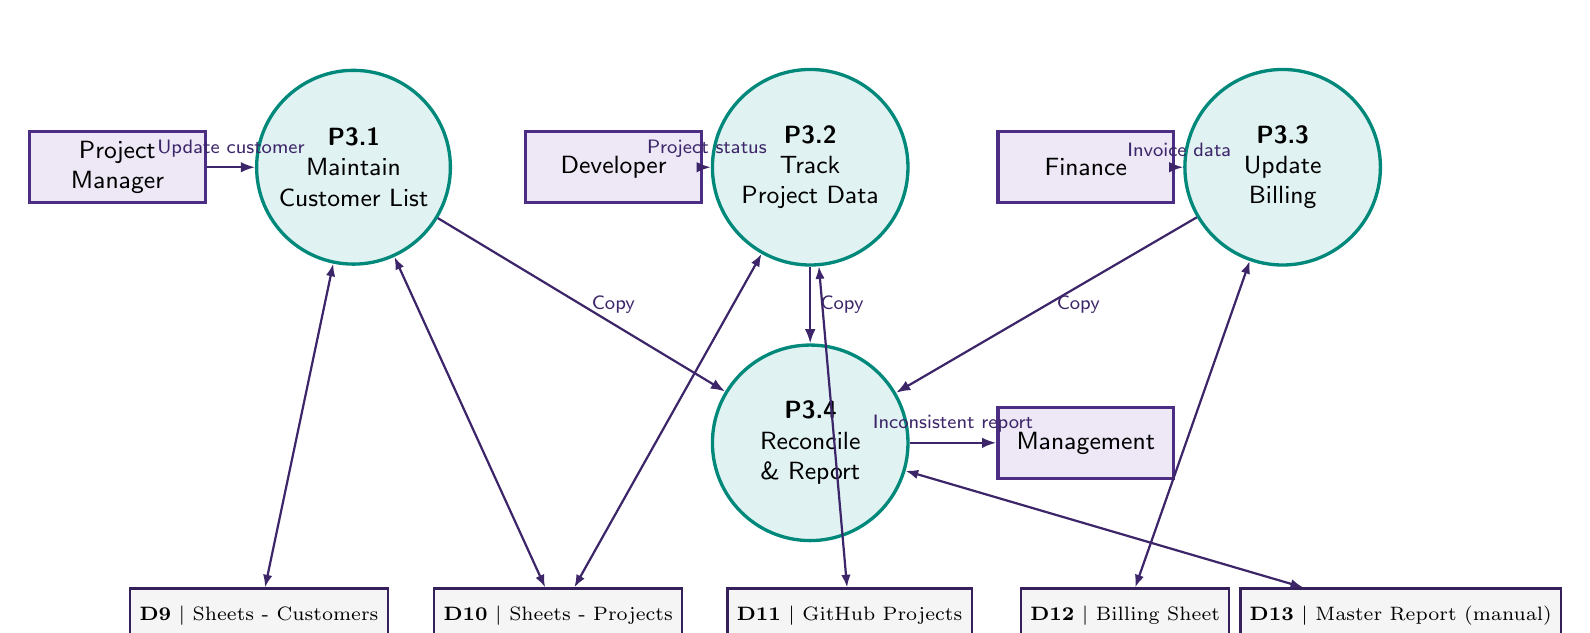
\begin{tikzpicture}[
    every node/.style={font=\sffamily\small},
    entity/.style={rectangle, draw=primary, fill=secondary, very thick, text width=2.0cm, align=center, minimum height=0.9cm},
    proc/.style={circle, draw=accent, fill=softteal, very thick, text width=1.9cm, align=center, minimum size=2.15cm},
    flow/.style={-{Latex[length=1.8mm]}, thick, color=primary!80!black},
    store/.style={thick, color=primary!70!black},
    flab/.style={font=\scriptsize\sffamily, align=center}
]
% Entities
\node[entity] (pm)   at (-2.8,4.5) {Project Manager};
\node[entity] (dev)  at (3.5,4.5)  {Developer};
\node[entity] (fin)  at (9.5,4.5)  {Finance};
\node[entity] (mgt)  at (9.5,1.0)  {Management};

% Processes
\node[proc] (p31) at (0.2,4.5)  {\textbf{P3.1}\\Maintain\\Customer List};
\node[proc] (p32) at (6.0,4.5)  {\textbf{P3.2}\\Track\\Project Data};
\node[proc] (p33) at (12.0,4.5) {\textbf{P3.3}\\Update\\Billing};
\node[proc] (p34) at (6.0,1.0)  {\textbf{P3.4}\\Reconcile\\\& Report};

% Multiple conflicting stores for the same data
\node[draw=primary!70!black, fill=softgray, thick, minimum width=2.8cm, minimum height=0.7cm, align=center, font=\scriptsize] (d9)  at (-1.0,-1.2) {\textbf{D9} \textbar{} Sheets - Customers};
\node[draw=primary!70!black, fill=softgray, thick, minimum width=2.6cm, minimum height=0.7cm, align=center, font=\scriptsize] (d10) at (2.8,-1.2) {\textbf{D10} \textbar{} Sheets - Projects};
\node[draw=primary!70!black, fill=softgray, thick, minimum width=2.5cm, minimum height=0.7cm, align=center, font=\scriptsize] (d11) at (6.5,-1.2) {\textbf{D11} \textbar{} GitHub Projects};
\node[draw=primary!70!black, fill=softgray, thick, minimum width=2.6cm, minimum height=0.7cm, align=center, font=\scriptsize] (d12) at (10.0,-1.2) {\textbf{D12} \textbar{} Billing Sheet};
\node[draw=primary!70!black, fill=softgray, thick, minimum width=2.7cm, minimum height=0.7cm, align=center, font=\scriptsize] (d13) at (13.5,-1.2) {\textbf{D13} \textbar{} Master Report (manual)};

% Flows showing duplication
\draw[flow] (pm) -- (p31) node[flab,midway,above]{Update customer};
\draw[flow] (dev) -- (p32) node[flab,midway,above]{Project status};
\draw[flow] (fin) -- (p33) node[flab,midway,above]{Invoice data};
\draw[flow] (p31) -- (p34) node[flab,midway,right]{Copy};
\draw[flow] (p32) -- (p34) node[flab,midway,right]{Copy};
\draw[flow] (p33) -- (p34) node[flab,midway,right]{Copy};
\draw[flow] (p34) -- (mgt) node[flab,midway,above]{Inconsistent report};

% All stores are written independently
\draw[flow,{Latex[length=1.6mm]}-{Latex[length=1.6mm]}] (p31) -- (d9);
\draw[flow,{Latex[length=1.6mm]}-{Latex[length=1.6mm]}] (p31) -- (d10);
\draw[flow,{Latex[length=1.6mm]}-{Latex[length=1.6mm]}] (p32) -- (d10);
\draw[flow,{Latex[length=1.6mm]}-{Latex[length=1.6mm]}] (p32) -- (d11);
\draw[flow,{Latex[length=1.6mm]}-{Latex[length=1.6mm]}] (p33) -- (d12);
\draw[flow,{Latex[length=1.6mm]}-{Latex[length=1.6mm]}] (p34) -- (d13);
\end{tikzpicture}
}
\caption{Level~1 DFD — Problem 3: Data Management \& Governance Deficiencies}
\label{fig:dfd_prob3}
\end{figure}

\begin{problemBox}
\textbf{Key problems visible:} The same core entities (customers, projects, billing) are maintained independently in at least five different stores. No canonical record exists. Reconciliation is entirely manual and error-prone.
\end{problemBox}

% ========================================================
% PROBLEM 4: Security & Access Control Risks
% ========================================================
\paragraph{D. Level 1 DFD — Problem 4: Security \& Access Control Risks}

This diagram (Figure~\ref{fig:dfd_prob4}) highlights how sensitive information travels through the same insecure, unaudited channels used for everyday conversation, with no role-based controls or logging.

\begin{figure}[H]
\centering
\resizebox{\textwidth}{!}{
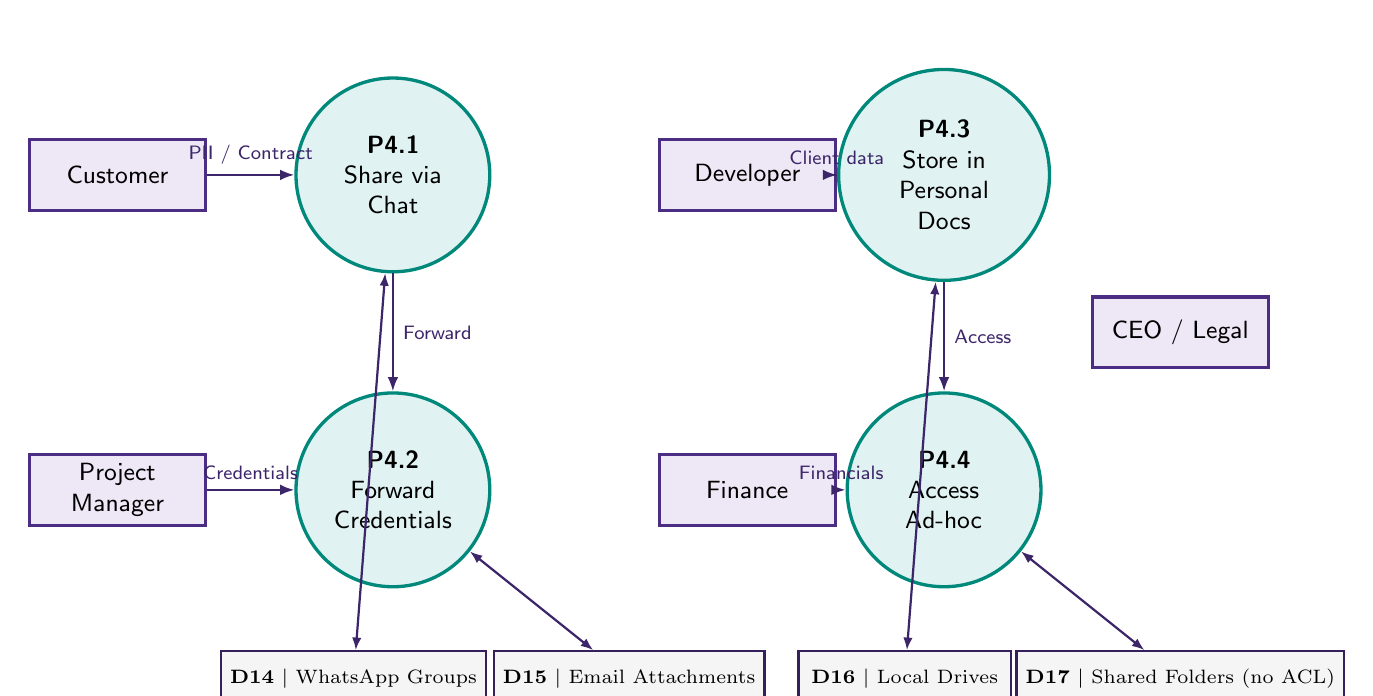
\begin{tikzpicture}[
    every node/.style={font=\sffamily\small},
    entity/.style={rectangle, draw=primary, fill=secondary, very thick, text width=2.0cm, align=center, minimum height=0.9cm},
    proc/.style={circle, draw=accent, fill=softteal, very thick, text width=1.9cm, align=center, minimum size=2.15cm},
    flow/.style={-{Latex[length=1.8mm]}, thick, color=primary!80!black},
    store/.style={thick, color=primary!70!black},
    flab/.style={font=\scriptsize\sffamily, align=center}
]
% Entities
\node[entity] (cust) at (-2.5,5.0) {Customer};
\node[entity] (pm)   at (-2.5,1.0) {Project Manager};
\node[entity] (dev)  at (5.5,5.0)  {Developer};
\node[entity] (fin)  at (5.5,1.0)  {Finance};
\node[entity] (ceo)  at (11.0,3.0) {CEO / Legal};

% Processes
\node[proc] (p41) at (1.0,5.0)  {\textbf{P4.1}\\Share via\\Chat};
\node[proc] (p42) at (1.0,1.0)  {\textbf{P4.2}\\Forward\\Credentials};
\node[proc] (p43) at (8.0,5.0)  {\textbf{P4.3}\\Store in\\Personal Docs};
\node[proc] (p44) at (8.0,1.0)  {\textbf{P4.4}\\Access\\Ad-hoc};

% Uncontrolled stores
\node[draw=primary!70!black, fill=softgray, thick, minimum width=2.8cm, minimum height=0.7cm, align=center, font=\scriptsize] (d14) at (0.5,-1.4) {\textbf{D14} \textbar{} WhatsApp Groups};
\node[draw=primary!70!black, fill=softgray, thick, minimum width=2.6cm, minimum height=0.7cm, align=center, font=\scriptsize] (d15) at (4.0,-1.4) {\textbf{D15} \textbar{} Email Attachments};
\node[draw=primary!70!black, fill=softgray, thick, minimum width=2.7cm, minimum height=0.7cm, align=center, font=\scriptsize] (d16) at (7.5,-1.4) {\textbf{D16} \textbar{} Local Drives};
\node[draw=primary!70!black, fill=softgray, thick, minimum width=2.5cm, minimum height=0.7cm, align=center, font=\scriptsize] (d17) at (11.0,-1.4) {\textbf{D17} \textbar{} Shared Folders (no ACL)};

% Sensitive flows
\draw[flow] (cust) -- (p41) node[flab,midway,above]{PII / Contract};
\draw[flow] (pm) -- (p42) node[flab,midway,above]{Credentials};
\draw[flow] (p41) -- (p42) node[flab,midway,right]{Forward};
\draw[flow] (dev) -- (p43) node[flab,midway,above]{Client data};
\draw[flow] (fin) -- (p44) node[flab,midway,above]{Financials};
\draw[flow] (p43) -- (p44) node[flab,midway,right]{Access};

% No controls on stores
\draw[flow,{Latex[length=1.6mm]}-{Latex[length=1.6mm]}] (p41) -- (d14);
\draw[flow,{Latex[length=1.6mm]}-{Latex[length=1.6mm]}] (p42) -- (d15);
\draw[flow,{Latex[length=1.6mm]}-{Latex[length=1.6mm]}] (p43) -- (d16);
\draw[flow,{Latex[length=1.6mm]}-{Latex[length=1.6mm]}] (p44) -- (d17);
\end{tikzpicture}
}
\caption{Level~1 DFD — Problem 4: Security \& Access Control Risks}
\label{fig:dfd_prob4}
\end{figure}

\begin{problemBox}
\textbf{Key problems visible:} Sensitive data (PII, credentials, contracts) flows through the same unaudited channels as casual chat. There are no access controls, no audit logs, and no distinction between public and confidential information.
\end{problemBox}

% ========================================================
% PROBLEM 5: Scalability & Operational Bottlenecks
% ========================================================
\paragraph{E. Level 1 DFD — Problem 5: Scalability \& Operational Bottlenecks}

This diagram (Figure~\ref{fig:dfd_prob5}) shows the extreme centralisation of coordination and decision-making around a very small number of individuals (primarily the Project Manager), making the entire operation dependent on their availability.

\begin{figure}[H]
\centering
\resizebox{\textwidth}{!}{
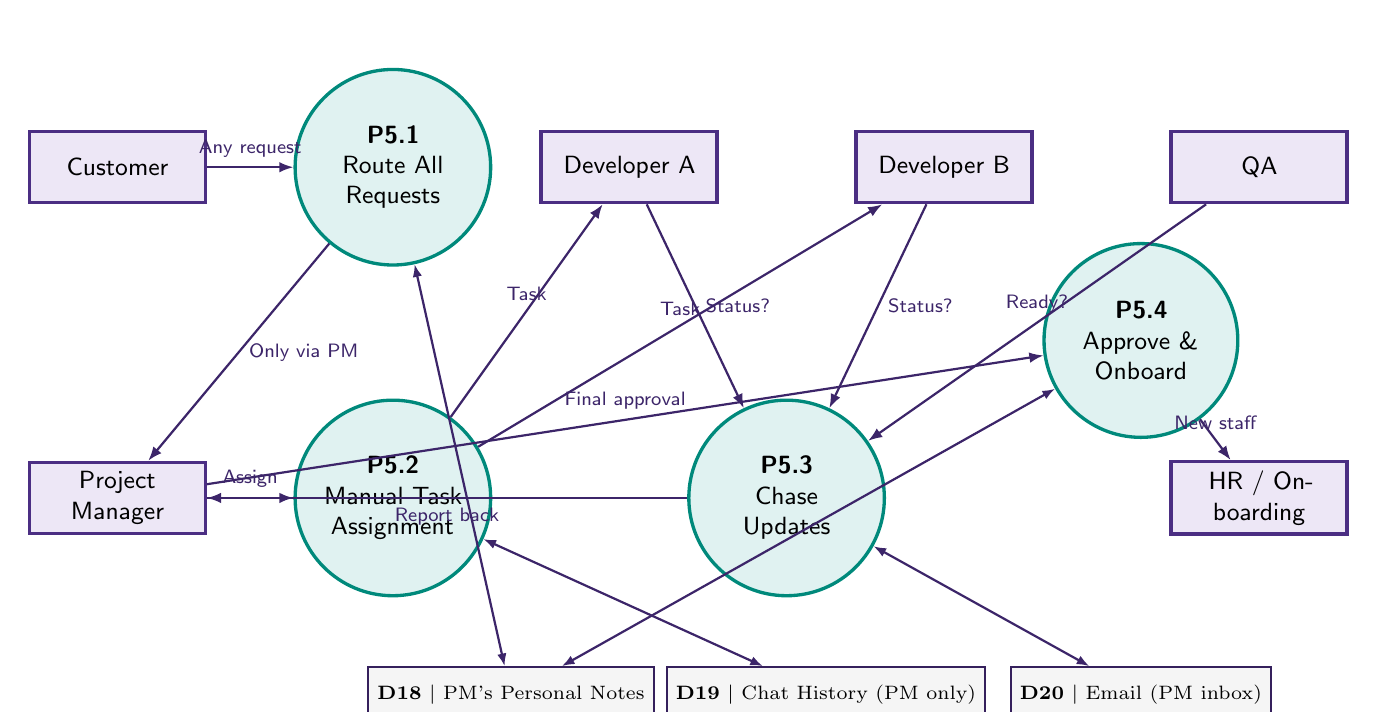
\begin{tikzpicture}[
    every node/.style={font=\sffamily\small},
    entity/.style={rectangle, draw=primary, fill=secondary, very thick, text width=2.0cm, align=center, minimum height=0.9cm},
    proc/.style={circle, draw=accent, fill=softteal, very thick, text width=1.9cm, align=center, minimum size=2.15cm},
    flow/.style={-{Latex[length=1.8mm]}, thick, color=primary!80!black},
    store/.style={thick, color=primary!70!black},
    flab/.style={font=\scriptsize\sffamily, align=center}
]
% Entities
\node[entity] (cust) at (-3.5,5.2) {Customer};
\node[entity] (pm)   at (-3.5,1.0) {Project Manager};
\node[entity] (dev1) at (3.0,5.2)  {Developer A};
\node[entity] (dev2) at (7.0,5.2)  {Developer B};
\node[entity] (qa)   at (11.0,5.2) {QA};
\node[entity] (hr)   at (11.0,1.0) {HR / Onboarding};

% Processes (all funnelling through PM)
\node[proc] (p51) at (0.0,5.2)  {\textbf{P5.1}\\Route All\\Requests};
\node[proc] (p52) at (0.0,1.0)  {\textbf{P5.2}\\Manual Task\\Assignment};
\node[proc] (p53) at (5.0,1.0)  {\textbf{P5.3}\\Chase\\Updates};
\node[proc] (p54) at (9.5,3.0)  {\textbf{P5.4}\\Approve \&\\Onboard};

% Bottleneck stores
\node[draw=primary!70!black, fill=softgray, thick, minimum width=2.8cm, minimum height=0.7cm, align=center, font=\scriptsize] (d18) at (1.5,-1.5) {\textbf{D18} \textbar{} PM's Personal Notes};
\node[draw=primary!70!black, fill=softgray, thick, minimum width=2.6cm, minimum height=0.7cm, align=center, font=\scriptsize] (d19) at (5.5,-1.5) {\textbf{D19} \textbar{} Chat History (PM only)};
\node[draw=primary!70!black, fill=softgray, thick, minimum width=2.7cm, minimum height=0.7cm, align=center, font=\scriptsize] (d20) at (9.5,-1.5) {\textbf{D20} \textbar{} Email (PM inbox)};

% All coordination arrows go through PM processes
\draw[flow] (cust) -- (p51) node[flab,midway,above]{Any request};
\draw[flow] (p51) -- (pm) node[flab,midway,right]{Only via PM};
\draw[flow] (pm) -- (p52) node[flab,midway,above]{Assign};
\draw[flow] (p52) -- (dev1) node[flab,midway,above]{Task};
\draw[flow] (p52) -- (dev2) node[flab,midway,above]{Task};
\draw[flow] (dev1) -- (p53) node[flab,midway,right]{Status?};
\draw[flow] (dev2) -- (p53) node[flab,midway,right]{Status?};
\draw[flow] (qa) -- (p53) node[flab,midway,above]{Ready?};
\draw[flow] (p53) -- (pm) node[flab,midway,below]{Report back};
\draw[flow] (pm) -- (p54) node[flab,midway,above]{Final approval};
\draw[flow] (p54) -- (hr) node[flab,midway,above]{New staff};

% PM's personal stores
\draw[flow,{Latex[length=1.6mm]}-{Latex[length=1.6mm]}] (p51) -- (d18);
\draw[flow,{Latex[length=1.6mm]}-{Latex[length=1.6mm]}] (p52) -- (d19);
\draw[flow,{Latex[length=1.6mm]}-{Latex[length=1.6mm]}] (p53) -- (d20);
\draw[flow,{Latex[length=1.6mm]}-{Latex[length=1.6mm]}] (p54) -- (d18);
\end{tikzpicture}
}
\caption{Level~1 DFD — Problem 5: Scalability \& Operational Bottlenecks}
\label{fig:dfd_prob5}
\end{figure}

\begin{problemBox}
\textbf{Key problems visible:} Virtually every significant flow (task assignment, status chasing, approvals, onboarding) passes through the Project Manager. When the PM is unavailable or overloaded, the entire delivery pipeline stalls. Knowledge and authority are not distributed.
\end{problemBox}

\noindent Together, these five focused Level~1 diagrams, along with the Context Diagram, expose the structural roots of all five organisational problems identified in Chapter~1. They establish a clear analytical baseline against which the proposed centralised information system will be designed in subsequent chapters.

% ================================================================
% END OF REPLACEMENT DFD SECTION
% ================================================================

% ================================================================

% ================================================================
% START OF SECTION 4.4 — Detailed Feasibility Analysis and Recommendation
% ================================================================
\section{Detailed Feasibility Analysis and Recommendation}
\label{sec:detailed-feasibility-and-recommendation}

\subsection{Introduction}
The information-gathering activities, stakeholder interviews, questionnaires, charts, and Data
Flow Diagrams in the preceding sections established that NextStepBD's current operating model is
functional but structurally fragmented. The organisation relies on several disconnected platforms,
informal approval channels, manually reconciled records, and a small number of key individuals
who coordinate a large proportion of operational work. The purpose of this section is therefore
to move from problem description to a comparative feasibility judgement and to recommend a
concrete solution strategy that NextStepBD can implement within its technical, economic, and
operational constraints.

The analysis is anchored on the five priority problems identified in Chapter~1:
\begin{enumerate}[label=\arabic*., leftmargin=1.8em]
    \item Fragmented Communication and Collaboration;
    \item System Fragmentation and Lack of Integration;
    \item Data Management and Governance Deficiencies;
    \item Security and Access Control Risks; and
    \item Scalability and Operational Bottlenecks.
\end{enumerate}

For each problem the section summarises the root cause, the supporting evidence, the
performance impact, and the economic or organisational consequence. The next part evaluates
\textbf{three genuinely alternative solution strategies} that the organisation could adopt in
response: a \textbf{Buy} strategy based on an off-the-shelf enterprise suite, a
\textbf{Configure} strategy based on configuring existing best-of-breed tools around a small
integration core, and a \textbf{Build} strategy based on developing a custom central platform in
house. Each strategy is described in terms of the same five problems so that the comparison is
direct, and is then rated for technical, economic, operational, and schedule feasibility. A
comparative scoring table is used to select a recommended strategy. The detailed design of the
recommended strategy --- functional and non-functional requirements, data migration plan,
security architecture, rollout plan, testing and acceptance framework, and change management
--- is developed in Chapter~5 (Design).

\begin{figure}[H]
\centering
\resizebox{\textwidth}{!}{%
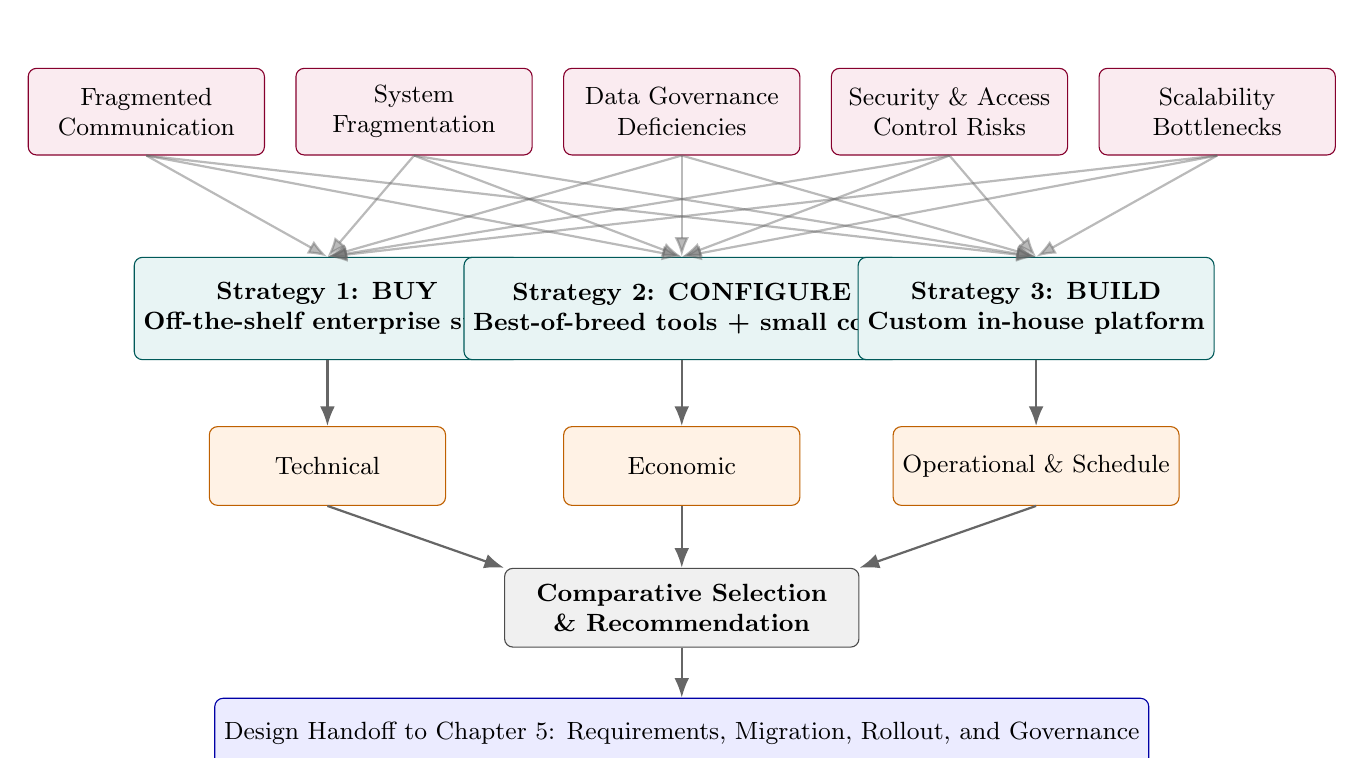
\begin{tikzpicture}[
    font=\small,
    problem/.style={draw=purple!70!black, rounded corners=3pt, fill=purple!8,
        minimum width=3.0cm, minimum height=1.1cm, align=center},
    strategy/.style={draw=teal!70!black, rounded corners=3pt, fill=teal!9,
        minimum width=4.0cm, minimum height=1.3cm, align=center, font=\small\bfseries},
    evaluate/.style={draw=orange!75!black, rounded corners=3pt, fill=orange!10,
        minimum width=3.0cm, minimum height=1.0cm, align=center},
    decision/.style={draw=black!70, rounded corners=3pt, fill=black!6,
        minimum width=4.5cm, minimum height=1.0cm, align=center, font=\small\bfseries},
    rollout/.style={draw=blue!65!black, rounded corners=3pt, fill=blue!8,
        minimum width=10.5cm, minimum height=0.9cm, align=center},
    arrow/.style={-{Latex[length=2.5mm]}, thick, draw=black!60}
]

% Five problems across the top
\node[problem] (p1) at (0,4.5) {Fragmented\\Communication};
\node[problem] (p2) at (3.4,4.5) {System\\Fragmentation};
\node[problem] (p3) at (6.8,4.5) {Data Governance\\Deficiencies};
\node[problem] (p4) at (10.2,4.5) {Security \& Access\\Control Risks};
\node[problem] (p5) at (13.6,4.5) {Scalability\\Bottlenecks};

% Three candidate strategies below
\node[strategy] (Sbuy)  at (2.3,2.0) {Strategy 1: \textbf{BUY}\\Off-the-shelf enterprise suite};
\node[strategy] (Sconf) at (6.8,2.0) {Strategy 2: \textbf{CONFIGURE}\\Best-of-breed tools + small core};
\node[strategy] (Sbuild) at (11.3,2.0) {Strategy 3: \textbf{BUILD}\\Custom in-house platform};

% Feasibility lenses applied to each strategy
\node[evaluate] (T) at (2.3,0.0) {Technical};
\node[evaluate] (E) at (6.8,0.0) {Economic};
\node[evaluate] (O) at (11.3,0.0) {Operational \& Schedule};

% Decision
\node[decision] (D) at (6.8,-1.8) {Comparative Selection\\\& Recommendation};

% Design handoff (elaborated in Chapter 5)
\node[rollout] (R) at (6.8,-3.4) {Design Handoff to Chapter 5: Requirements, Migration, Rollout, and Governance};

% Connections: each problem informs each strategy
\foreach \p in {p1,p2,p3,p4,p5}{
    \draw[arrow, opacity=0.45] (\p.south) -- (Sbuy.north);
    \draw[arrow, opacity=0.45] (\p.south) -- (Sconf.north);
    \draw[arrow, opacity=0.45] (\p.south) -- (Sbuild.north);
}
% Strategies feed evaluation
\draw[arrow] (Sbuy.south)  -- (T.north);
\draw[arrow] (Sconf.south)  -- (E.north);
\draw[arrow] (Sbuild.south) -- (O.north);
% Evaluation to decision
\draw[arrow] (T.south) -- (D.north west);
\draw[arrow] (E.south) -- (D.north);
\draw[arrow] (O.south) -- (D.north east);
% Decision to rollout
\draw[arrow] (D.south) -- (R.north);

\end{tikzpicture}%
}
\caption{Comparative Feasibility Framework --- Three Alternative Solution Strategies
         for the Five Identified Problems}
\label{fig:feasibility-framework}
\end{figure}

% ----------------------------------------------------------------
\subsection{Root Cause Analysis of Identified Problems}
\label{subsec:root-cause-analysis}

The five problems identified in Chapter~1 do not operate independently. Communication gaps
create incomplete records, incomplete records increase fragmentation, fragmented data weakens
access control and reporting, and all four conditions increase dependence on project managers and
senior engineers. Selecting one visible problem and treating it in isolation would therefore
produce only temporary improvement. The root causes summarised below are the analytical baseline
against which the three solution strategies are evaluated.

\subsubsection{Problem 01: Fragmented Communication and Collaboration}
\textbf{Root cause.} Informal communication tools are used both for conversation and as a de
facto system of record. Client requirements, approvals, clarifications, and delivery
confirmations may remain inside WhatsApp threads, email messages, or personal notes instead of
being linked to formal project artefacts. The project manager frequently becomes the human
routing layer between clients, developers, QA personnel, finance, and management.

\textbf{Evidence from information gathering.} The employee analysis produced a low average score
of 2.4 for communication and approval clarity. The Engineering Manager also rated
approval-channel clarity and the sufficiency of chat approvals at 2 out of 5. Customers remained
broadly satisfied but expressed a preference for formal approval mechanisms and access to
historical confirmations. The DFD in Figure~\ref{fig:dfd_prob1} shows approvals distributed
across WhatsApp, email, and project notes without a single traceable record.

\textbf{Performance impact.} Repeated clarification cycles, delayed task initiation,
misinterpretation of scope and acceptance criteria, weak traceability during scope disputes and
billing verification, and increased context switching for developers and account leads.

\textbf{Economic and organisational impact.} Hidden labour cost through repeated meetings,
message searching, manual confirmation, and rework; delayed approvals postpone delivery and
billing; unrecovered scope expansion during client disputes.

\subsubsection{Problem 02: System Fragmentation and Lack of Integration}
\textbf{Root cause.} NextStepBD uses WhatsApp, Slack, email, GitHub, Excel, Google Sheets, shared
documents, and project-specific scripts as separate operational tools. These platforms are useful
individually, but the current environment has no common integration layer or canonical record
that keeps project, task, approval, billing, and delivery information synchronised.

\textbf{Evidence from information gathering.} System fragmentation produced one of the strongest
negative signals in the employee survey (average problem score 4.2). The Engineering Manager
also reported high levels of cross-tool reconciliation and data copying. The DFD in
Figure~\ref{fig:dfd_prob2} demonstrates that management reporting requires aggregation from
Google Sheets, GitHub, and manual documents.

\textbf{Performance impact.} Duplicate data entry, inconsistent updates, slow reporting,
synchronisation failures, missing tasks or status changes, and reduced management visibility.

\textbf{Economic and organisational impact.} Manual reconciliation consumes delivery time; the
cost of maintaining disconnected systems rises almost linearly with the number of clients.

\subsubsection{Problem 03: Data Management and Governance Deficiencies}
\textbf{Root cause.} The organisation lacks a formally governed data model for customers,
projects, requirements, approvals, tasks, invoices, and support incidents. The same information
may appear in multiple spreadsheets or documents with different identifiers, formats, and levels
of completeness. Data ownership, validation rules, retention periods, and change history are not
consistently defined.

\textbf{Evidence from information gathering.} The employee survey produced an average score of
2.53 for data governance, and confidence in billing-record accuracy was concentrated at the
lower end of the scale. Management reported only moderate visibility into project risk, while HR
identified weak knowledge and capacity tracking. The absence of a single source of truth is
visible in the current-state DFDs.

\textbf{Performance impact.} Conflicting records, weak reporting accuracy, delayed managerial
decisions, difficulty linking requirements, approvals, tasks, deliverables, and invoices, and
limited ability to measure delivery performance consistently.

\textbf{Economic and organisational impact.} Direct billing risk and indirect administrative
cost; weakened forecasting, profitability analysis, and audit readiness; future integrations
reproduce existing inconsistencies if a governed model is not introduced.

\subsubsection{Problem 04: Security and Access Control Risks}
\textbf{Root cause.} Sensitive client information, credentials, screenshots, and personal data
may be shared through informal channels or stored on personal devices. Access control differs by
tool, and the company cannot consistently demonstrate who accessed, changed, exported, or deleted
a record. Secrets management, redaction, retention, and audit logging are not uniformly
enforced.

\textbf{Evidence from information gathering.} The employee security score was 3.07, indicating
moderate but material concern. Survey results showed that some employees save client messages
locally or need to redact client information. Stakeholder interviews also raised concerns about
PII, credential handling, role-based access, and the difficulty of retrofitting SSO across
legacy tools.

\textbf{Performance impact.} Slower incident response, risk of unauthorised access or
accidental disclosure, inconsistent security practices, difficulty revoking access, and reduced
confidence in the integrity of client and operational records.

\textbf{Economic and organisational impact.} A security incident can produce legal cost, service
disruption, contractual penalties, client loss, and reputational damage. Weak auditability
reduces eligibility for enterprise work and increases the effort required to respond to client
security reviews.

\subsubsection{Problem 05: Scalability and Operational Bottlenecks}
\textbf{Root cause.} Routine task assignment, approval routing, onboarding, escalation,
reporting, and coordination are concentrated in a small number of managers and senior staff.
Processes are not consistently supported by templates, role-based assignment, skills data,
automated reminders, or measurable service levels. Organisational knowledge therefore remains
person-dependent.

\textbf{Evidence from information gathering.} HR reported weak capacity visibility, skills
tracking, cross-training, and access to onboarding documents. Stakeholders indicated that
onboarding may require four to six weeks before a new employee becomes productive. At the same
time, employee automation readiness was very high, with an average score of 4.61, and all
responses to automation-related questions were at ``agree'' or ``strongly agree''.

\textbf{Performance impact.} Delayed decisions when key staff are unavailable, inconsistent task
assignment, long onboarding time, increased notification noise, and limited ability to increase
project volume without proportional management effort.

\textbf{Economic and organisational impact.} The organisation cannot scale efficiently when
every additional project requires more manual coordination. Key-person dependency raises
continuity risk and contributes to staff overload.

\begin{table}[H]
\centering
\caption{Root Cause Analysis Summary for NextStepBD}
\label{tab:root-cause-summary}
\small
\renewcommand{\arraystretch}{1.25}
\begin{tabularx}{\textwidth}{>{\raggedright\arraybackslash}p{2.7cm}
                                >{\raggedright\arraybackslash}p{3.6cm}
                                >{\raggedright\arraybackslash}X
                                >{\raggedright\arraybackslash}p{3.0cm}}
\toprule
\textbf{Problem} & \textbf{Primary Root Cause} & \textbf{Key Evidence} & \textbf{Main Consequence} \\
\midrule
Fragmented communication & Informal channels act as the system of record & Communication and approval score 2.4; approval clarity rated 2/5 & Rework, delay, and weak approval traceability \\
System fragmentation & No integration layer between operational tools & Fragmentation score 4.2; frequent reconciliation and copy-paste & High administrative effort and inconsistent status \\
Data governance deficiencies & No canonical model, ownership, or validation rules & Governance score 2.53; low billing confidence; multiple data stores & Unreliable reporting and billing risk \\
Security and access risks & Sensitive data handled across tools without consistent RBAC and audit & Security score 3.07; local storage and redaction concerns & Breach, compliance, and client-trust exposure \\
Scalability bottlenecks & Manual routing and key-person dependency & Onboarding takes 4--6 weeks; automation readiness 4.61 & Limited throughput and slow growth \\
\bottomrule
\end{tabularx}
\end{table}

\subsubsection{Cross-Problem Dependency and Prioritisation Analysis}
\label{sec:cross-problem-analysis}

A cause-and-effect review shows three structural layers. The \textbf{foundation layer} contains
identity, access, the canonical data model, audit history, backup, and integration rules. The
\textbf{process layer} contains requirement capture, approvals, task routing, escalation,
billing readiness, and onboarding. The \textbf{delivery layer} contains build, testing,
deployment, monitoring, incident response, and performance measurement. Improvement at the
delivery layer will remain fragile if the foundation and process layers are not addressed first.
The dependency chain indicates that the highest-leverage intervention is to establish a governed
information foundation and then formalise the workflows that create and update that information.
This layering is used as a lens for comparing the three candidate strategies in the next
section.

\begin{figure}[H]
\centering
\resizebox{0.96\textwidth}{!}{%
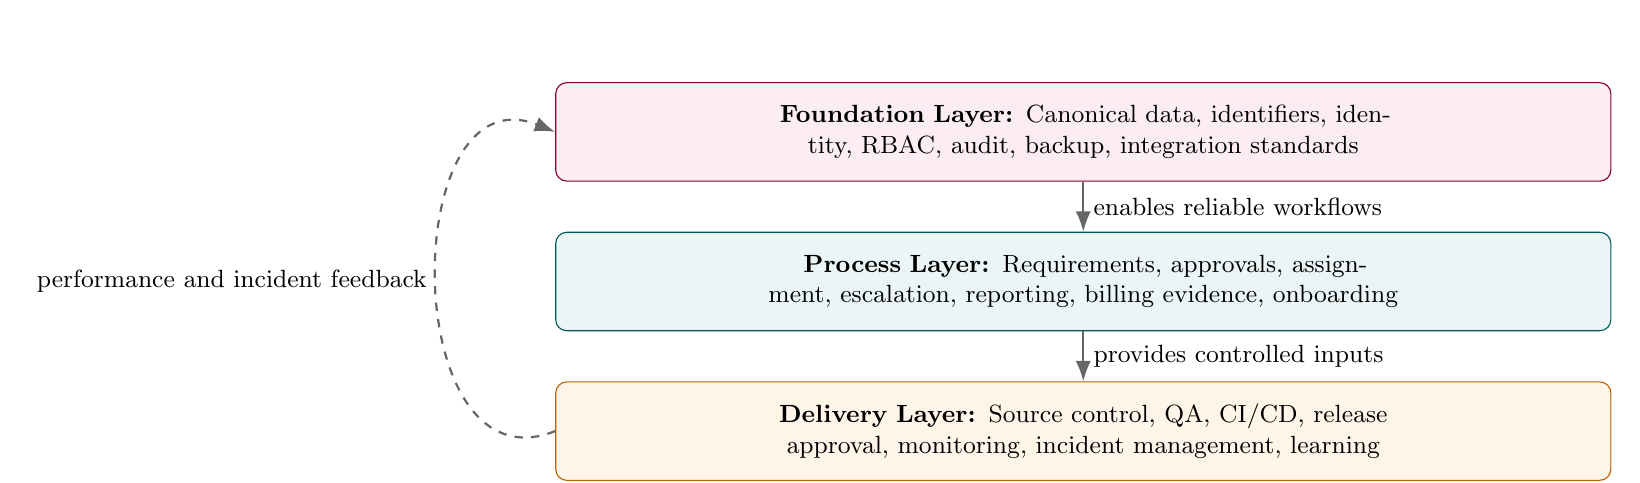
\begin{tikzpicture}[
    font=\small,
    layer/.style={draw=purple!70!black, rounded corners=4pt, minimum width=13.4cm,
        minimum height=1.25cm, align=center, fill=purple!7, text width=12.8cm},
    arrow/.style={-{Latex[length=2.6mm]}, thick, draw=black!60}
]
\node[layer] (foundation) at (0,0) {\textbf{Foundation Layer:} Canonical data, identifiers, identity, RBAC, audit, backup, integration standards};
\node[layer, fill=teal!8, draw=teal!70!black] (process) at (0,-1.9) {\textbf{Process Layer:} Requirements, approvals, assignment, escalation, reporting, billing evidence, onboarding};
\node[layer, fill=orange!9, draw=orange!75!black] (delivery) at (0,-3.8) {\textbf{Delivery Layer:} Source control, QA, CI/CD, release approval, monitoring, incident management, learning};
\draw[arrow] (foundation) -- node[right]{enables reliable workflows} (process);
\draw[arrow] (process) -- node[right]{provides controlled inputs} (delivery);
\draw[arrow, dashed] (delivery.west) .. controls +(-2.0,-.8) and +(-2.0,.8) .. node[left, align=center]{performance and incident feedback} (foundation.west);
\end{tikzpicture}%
}
\caption{Dependency Layers Connecting the Five Identified Problems}
\label{fig:dependency-layers}
\end{figure}

% ----------------------------------------------------------------
\subsection{Three Alternative Solution Strategies}
\label{subsec:alternative-strategies}

The five problems are interdependent. However, the organisation does not have to commit to a
single, predetermined stack before understanding the realistic options. The classical
information-systems decision space offers three strategic postures, each of which can in
principle address all five problems, but in very different ways and at very different cost,
risk, and time horizons. The strategies are described in the same order for every problem so
that the comparison that follows is direct.

\subsubsection{Strategy 1 --- Buy: Off-the-Shelf Enterprise Suite}
\label{sec:strategy-buy}

\textbf{Strategy description.} Replace the current patchwork with a single, integrated
enterprise suite such as an end-to-end Professional Services Automation (PSA) or Enterprise
Resource Planning (ERP) platform. The suite would natively cover customer records, project
planning, time tracking, approvals, billing, basic reporting, and access control. Existing
tools (Sheets, GitHub, WhatsApp) would be retained only for casual or specialised use, and the
suite would be the system of record for all five problem areas.

\textbf{Application to the five problems.}
\begin{itemize}[leftmargin=1.6em]
    \item \textbf{Communication:} the suite's approval, request, and notification modules
          displace chat as the official approval channel.
    \item \textbf{Fragmentation:} the suite replaces rather than integrates the disconnected
          tools, eliminating the integration gap but requiring users to migrate their workflows.
    \item \textbf{Data governance:} the suite's canonical schema, validation rules, and audit
          logs are used as-is, removing the need to design governance from scratch.
    \item \textbf{Security:} SSO, RBAC, audit, and retention are typically built in.
    \item \textbf{Scalability:} workflow templates, role-based assignment, and reporting are
          provided out of the box.
\end{itemize}

\textbf{Key advantage.} Shortest path to a governed end-to-end system; vendors provide
documentation, support, and continuous updates.

\textbf{Key disadvantage.} Suite workflows rarely match the way a small services company
actually works, so adoption friction is high; licences are recurring; customisation beyond
configuration is difficult and expensive; and lock-in risk is significant because data
extracts may be lossy or incomplete.

\subsubsection{Strategy 2 --- Configure: Best-of-Breed Tools Around a Small Integration Core}
\label{sec:strategy-configure}

\textbf{Strategy description.} Keep the team's preferred chat and development tools, configure
a best-of-breed collaboration and workflow tool (e.g., Jira, ClickUp, Notion, Linear) for task
and approval management, and connect everything to a small, narrowly scoped \emph{integration
core} that records canonical entities (customer, project, requirement, approval) and exchanges
data with the other tools through APIs and webhooks. A modest DevOps, QA, and observability
stack (CI/CD pipelines, monitoring, alerting) is layered on top using standard tooling.

\textbf{Application to the five problems.}
\begin{itemize}[leftmargin=1.6em]
    \item \textbf{Communication:} chat tools remain in use, but important decisions are
          \emph{captured} into the workflow tool or the integration core through a one-click
          confirmation or operator review.
    \item \textbf{Fragmentation:} the integration core is the single source of truth for the
          entities that matter most; selected fields are synchronised with Sheets, GitHub, and
          other tools.
    \item \textbf{Data governance:} the integration core defines the canonical schema, with
          validation, duplicate detection, provenance, and audit logging; data stewardship rules
          are written into the operating model.
    \item \textbf{Security:} SSO, RBAC, secrets management, and audit logs are introduced in
          the foundation release, with the workflow tool and integration core as control
          points.
    \item \textbf{Scalability:} workflow templates, role-based assignment, capacity tags, and
          standard onboarding checklists are configured in the workflow tool and connected to
          the canonical record.
\end{itemize}

\textbf{Key advantage.} Best fit to NextStepBD's existing skills, current tools, and
collaborative culture. The integration core is small, the workflow tool is familiar, and
adoption is incremental.

\textbf{Key disadvantage.} The integration core still needs to be designed, built, and
maintained; the organisation has to manage a multi-vendor environment; and the success of the
strategy depends heavily on disciplined configuration and process ownership.

\subsubsection{Strategy 3 --- Build: Custom In-House Central Platform}
\label{sec:strategy-build}

\textbf{Strategy description.} Develop a fully custom, in-house information platform that
ingests data from the current tools, normalises it into a rich canonical model, and exposes a
unified user interface for all five problem areas. Custom modules cover requirements,
approvals, task tracking, billing readiness, security, and reporting, and the platform is
extended with bespoke DevOps and observability capabilities over time.

\textbf{Application to the five problems.}
\begin{itemize}[leftmargin=1.6em]
    \item \textbf{Communication:} the custom platform can be designed to ingest and reflect
          chat content, allowing highly tailored approval capture.
    \item \textbf{Fragmentation:} all information is consolidated inside the platform, removing
          external integration gaps entirely.
    \item \textbf{Data governance:} the platform can encode exactly the governance rules the
          organisation wants, including provenance, audit, retention, and redaction.
    \item \textbf{Security:} the platform can implement any required control, with no
          constraint from a vendor's feature set.
    \item \textbf{Scalability:} the platform can be designed for the specific growth pattern of
          the business, with custom automation and routing rules.
\end{itemize}

\textbf{Key advantage.} Maximum control and the closest possible match to the organisation's
needs over the long term; no licence or vendor constraint; full ownership of data and
roadmap.

\textbf{Key disadvantage.} Highest cost, longest timeline, largest project risk. NextStepBD
would be diverting scarce engineering capacity from billable client work, and would have to
maintain every part of the system --- UI, integration, security, performance, recovery,
compliance --- itself.

% ----------------------------------------------------------------
\subsection{Comparative Feasibility Evaluation of the Three Strategies}
\label{sec:comparative-feasibility}

The three strategies are now compared on a common set of dimensions: technical feasibility,
economic feasibility, operational feasibility, schedule feasibility, and problem coverage.
Where useful, indicative cost is described in bands rather than exact figures, because the
final numbers depend on vendor selection, scope, and pilot outcomes.

\subsubsection{Problem Coverage Matrix}
\label{sec:coverage-matrix}

The matrix below scores each strategy's ability to address each of the five problems on a
four-point scale (\textbf{F}ull, \textbf{P}artial, \textbf{L}imited, \textbf{N}one). ``Full''
means the strategy natively addresses the problem; ``Partial'' means the strategy addresses it
but with caveats or residual manual steps; ``Limited'' means the strategy touches the problem
only indirectly; ``None'' means the strategy does not address the problem.

\begin{table}[H]
\centering
\caption{Problem Coverage Matrix for the Three Solution Strategies}
\label{tab:coverage-matrix}
\renewcommand{\arraystretch}{1.30}
\begin{tabularx}{\textwidth}{>{\raggedright\arraybackslash}p{3.6cm}
                                >{\centering\arraybackslash}p{2.0cm}
                                >{\centering\arraybackslash}p{2.4cm}
                                >{\centering\arraybackslash}p{2.4cm}}
\toprule
\textbf{Identified Problem} & \textbf{Strategy 1: Buy} & \textbf{Strategy 2: Configure} & \textbf{Strategy 3: Build} \\
\midrule
1. Fragmented Communication \& Collaboration & Partial & Full & Full \\
2. System Fragmentation \& Lack of Integration & Full & Full & Full \\
3. Data Management \& Governance Deficiencies & Full & Full & Full \\
4. Security \& Access Control Risks & Full & Partial & Full \\
5. Scalability \& Operational Bottlenecks & Partial & Full & Full \\
\midrule
\textbf{Overall coverage} & \textbf{High, with two partials} & \textbf{High, one partial} & \textbf{Highest, but at highest cost} \\
\bottomrule
\end{tabularx}
\end{table}

The matrix shows that all three strategies can, in principle, address all five problems. The
differences are not in \emph{whether} they address each problem, but in \emph{how completely}
they do so, \emph{at what cost}, and \emph{on what timeline}. The next subsections evaluate
those differences.

\subsubsection{Technical Feasibility Comparison}
\label{sec:technical-comparison}

\textbf{Strategy 1 (Buy).} Technically the lowest effort for NextStepBD, because the
infrastructure and core code are owned by the vendor. However, the organisation must still
integrate the suite with any tool that is intentionally kept (for example, GitHub), and must
customise the suite's data model and workflow to its own terminology. Suitability depends on
whether a vendor's configuration options can support a small, project-driven services
company, which is a market that is often underserved by larger enterprise suites.

\textbf{Strategy 2 (Configure).} Technically feasible with a small, focused engineering team.
A canonical data store, a thin integration core, a configured collaboration tool, and standard
DevOps tooling are all well-understood technologies. The architecture is modular and can be
introduced without replacing all existing tools. The constraint is that engineering time
remains limited and must be balanced against billable work.

\textbf{Strategy 3 (Build).} Technically the most demanding. The organisation must design,
implement, test, secure, scale, and maintain every component: ingestion, normalisation,
workflow engine, user interface, integrations, security, observability, and recovery.
Technical risk is concentrated in two areas: the long development timeline (during which
requirements may shift) and the long maintenance tail (during which the in-house team becomes
permanently responsible for operational reliability).

\begin{table}[H]
\centering
\caption{Technical Feasibility by Strategy}
\label{tab:tech-feasibility}
\small
\renewcommand{\arraystretch}{1.20}
\begin{tabularx}{\textwidth}{>{\raggedright\arraybackslash}p{3.2cm}
                                >{\centering\arraybackslash}p{1.8cm}
                                >{\raggedright\arraybackslash}X}
\toprule
\textbf{Strategy} & \textbf{Rating} & \textbf{Reason} \\
\midrule
Strategy 1: Buy & Medium--High & Lowest in-house effort; constrained by vendor feature set and configuration ceiling \\
Strategy 2: Configure & High & Modular architecture, mature components, fits the team's skills \\
Strategy 3: Build & Medium & High ambition, but high in-house responsibility and long technical runway \\
\bottomrule
\end{tabularx}
\end{table}

\subsubsection{Economic Feasibility Comparison}
\label{sec:economic-comparison}

Costs are described in three bands relative to NextStepBD's size and budget:
\textbf{Low} (recurring licence plus light implementation), \textbf{Medium} (combination of
licence, configuration, and modest engineering), and \textbf{High} (significant engineering
plus the opportunity cost of diverted billable capacity).

\textbf{Strategy 1 (Buy).} Total cost depends heavily on licence model. Per-seat enterprise
suites for ~50 users with the modules required for NextStepBD typically sit in the
\textbf{Medium--High} band when summed over three years. Implementation services from the
vendor or a partner are a separate, often significant, line item. Operational savings come
from reduced reconciliation and faster reporting, but are partly offset by per-seat fees and
future price increases.

\textbf{Strategy 2 (Configure).} Most of the cost is internal engineering time plus
subscriptions for the configured collaboration tool and any managed iPaaS, identity, or
observability services. Total cost is typically in the \textbf{Medium} band, with the
advantage that cost scales with usage rather than seat count and that the in-house team
develops reusable capability that lowers future cost.

\textbf{Strategy 3 (Build).} Highest cost. In addition to infrastructure and tools, the
organisation must fund a multi-quarter engineering programme and absorb the opportunity cost
of diverted billable capacity. Cost is typically in the \textbf{High} band for the first two
to three years. Long-term operating cost may be lower than Strategy 1, but the upfront
investment and risk-adjusted return are unfavourable for a 50-person services company.

\begin{table}[H]
\centering
\caption{Indicative Cost and Benefit by Strategy}
\label{tab:cost-comparison}
\small
\renewcommand{\arraystretch}{1.18}
\begin{tabularx}{\textwidth}{>{\raggedright\arraybackslash}p{3.2cm}
                                >{\raggedright\arraybackslash}X
                                >{\raggedright\arraybackslash}X}
\toprule
\textbf{Dimension} & \textbf{Strategy 1: Buy} & \textbf{Strategy 2: Configure} \\
\midrule
Year-1 cost & High (licence + implementation) & Medium (engineering + selected subscriptions) \\
Ongoing cost & Recurring licence that scales with seats & Lower recurring cost; mainly internal maintenance \\
Time-to-value & Moderate (depends on implementation partner) & Fast for the pilot, slower for full rollout \\
Switching cost & High (data and process lock-in) & Moderate (open APIs and portable identifiers) \\
\midrule
\textbf{Dimension} & \textbf{Strategy 3: Build} & \textbf{Notes} \\
\midrule
Year-1 cost & Highest (large engineering programme) & Diverts significant capacity from billable work \\
Ongoing cost & Lower per-user, but high maintenance burden & Permanent platform team required \\
Time-to-value & Slowest (typically 9--18 months to a useful pilot) & Value delivered late, with high reversal cost \\
Switching cost & Low (organisation owns the code) & Requires sustained engineering investment \\
\bottomrule
\end{tabularx}
\end{table}

\subsubsection{Operational Feasibility Comparison}
\label{sec:operational-comparison}

\textbf{Strategy 1 (Buy).} Operational fit depends on how closely the suite's workflows match
the way a small services company actually works. A general-purpose suite may impose process
discipline that the team experiences as additional overhead, and the long adoption curve
(common in suite rollouts) can be demoralising for a 50-person team used to informal,
fast-moving practice. Support scores in Section~4.3 are positive, but they reflect openness
to improvement in general, not endorsement of a specific suite.

\textbf{Strategy 2 (Configure).} Best operational fit for NextStepBD. The configured
collaboration tool is familiar to most users, chat tools are preserved, and the integration
core is invisible to end users. The main operational task is not switching tools but changing
habits: capturing important decisions, using templates, and retiring duplicate manual
records. Stakeholder support scores (CEO 5, HR 4, Engineering Manager 4, employees 4.73,
customers 4) indicate strong endorsement for this kind of process standardisation.

\textbf{Strategy 3 (Build).} Operational risk is highest. A custom platform must be learned,
trusted, and operated by a 50-person team that has limited spare capacity. Even a successful
build leaves the team dependent on a small group of in-house developers for ongoing
maintenance, reproducing the same key-person dependency the strategy is meant to remove.

\subsubsection{Schedule Feasibility Comparison}
\label{sec:schedule-comparison}

The three strategies have very different realistic timelines. The phased pilot described later
in this section is sized for Strategy 2; the same pilot would be considerably shorter for
Strategy 1 (because there is less to build) and considerably longer for Strategy 3 (because
there is more).

\begin{table}[H]
\centering
\caption{Indicative Timeline and Pilot Effort by Strategy}
\label{tab:schedule-comparison}
\small
\renewcommand{\arraystretch}{1.18}
\begin{tabularx}{\textwidth}{>{\raggedright\arraybackslash}p{3.2cm}
                                >{\raggedright\arraybackslash}X
                                >{\raggedright\arraybackslash}p{2.4cm}}
\toprule
\textbf{Strategy} & \textbf{Realistic Pilot Timeline} & \textbf{Full Rollout Estimate} \\
\midrule
Strategy 1: Buy & 3--4 months to a working pilot & 9--12 months organisation-wide \\
Strategy 2: Configure & 4--6 months to a working pilot & 6--9 months organisation-wide \\
Strategy 3: Build & 9--12 months to a working pilot & 18--24 months organisation-wide \\
\bottomrule
\end{tabularx}
\end{table}

\subsubsection{Weighted Comparative Scoring}
\label{sec:weighted-scoring}

The five feasibility dimensions are weighted to reflect the organisation's priorities: cost
control and operational fit are weighted highest because they most directly determine whether
the chosen strategy will actually be used; technical and schedule feasibility are weighted
moderately; and problem coverage is treated as a minimum entry condition (any strategy that
does not address all five problems at least partially is excluded).

\begin{table}[H]
\centering
\caption{Weighted Comparative Scoring of the Three Strategies}
\label{tab:weighted-scoring}
\renewcommand{\arraystretch}{1.20}
\begin{tabularx}{\textwidth}{>{\raggedright\arraybackslash}p{3.6cm}
                                >{\centering\arraybackslash}p{1.4cm}
                                >{\centering\arraybackslash}p{1.4cm}
                                >{\centering\arraybackslash}p{1.4cm}
                                >{\raggedright\arraybackslash}p{3.0cm}}
\toprule
\textbf{Decision Criterion (weight)} & \textbf{Buy} & \textbf{Configure} & \textbf{Build} & \textbf{Comment} \\
\midrule
Problem coverage (20\%) & 4 & 5 & 5 & All three are acceptable; Configure and Build are strongest \\
Technical feasibility (15\%) & 3 & 5 & 3 & Configure uses mature components directly in the team's skills \\
Economic feasibility (25\%) & 2 & 4 & 2 & Configure is the lowest realistic total cost for a 50-person services company \\
Operational feasibility (25\%) & 3 & 5 & 3 & Configure best matches existing culture and skills \\
Schedule feasibility (15\%) & 4 & 4 & 2 & Configure delivers a useful pilot in a realistic timeframe \\
\midrule
\textbf{Weighted total (out of 5)} & \textbf{3.05} & \textbf{4.60} & \textbf{3.00} & \textbf{Configure leads clearly} \\
\bottomrule
\end{tabularx}
\end{table}

The weighted comparison makes the recommendation unambiguous for NextStepBD's current size,
skill mix, and operational profile. \textbf{Strategy 2 (Configure) is the recommended
solution strategy.} The remainder of this section describes how the recommended strategy is
operationalised, not how the alternatives could be combined.

% ----------------------------------------------------------------
\subsection{Recommended Solution: Strategy 2 --- Configure}
\label{sec:recommended-strategy}

The recommended strategy is to configure best-of-breed tools around a small, narrowly scoped
integration core, with the architecture depicted in Figure~\ref{fig:integrated-target-architecture}.
The integration core holds the canonical record of customers, projects, requirements,
approvals, tasks, billing status, and key capacity data; a configured collaboration and
workflow tool provides the human-facing workspace; and a DevOps, QA, and observability stack
provides delivery reliability. Identity, RBAC, audit, redaction, data quality, backup, and
monitoring operate as cross-cutting controls across all three layers.

\begin{figure}[H]
\centering
\resizebox{0.98\textwidth}{!}{%
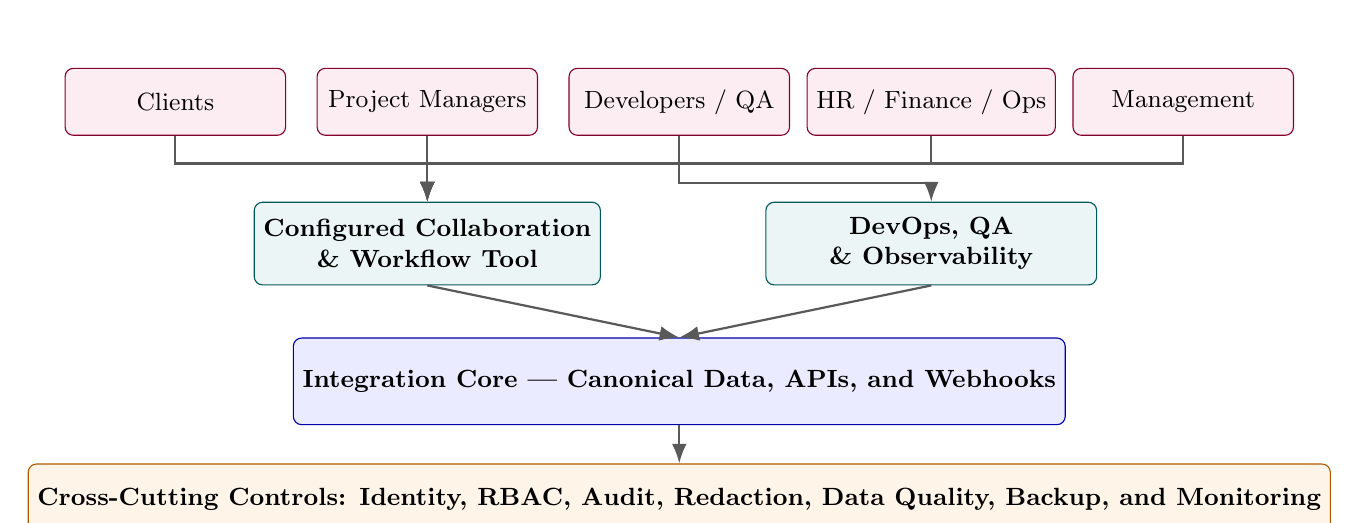
\begin{tikzpicture}[
    font=\small,
    box/.style={draw=teal!70!black, rounded corners=3pt, fill=teal!8,
        minimum width=4.2cm, minimum height=1.05cm, align=center, font=\small\bfseries},
    user/.style={draw=purple!70!black, rounded corners=3pt, fill=purple!7,
        minimum width=2.8cm, minimum height=.85cm, align=center},
    cross/.style={draw=orange!70!black, rounded corners=3pt, fill=orange!9,
        minimum width=12.0cm, minimum height=.9cm, align=center, font=\small\bfseries},
    core/.style={draw=blue!65!black, rounded corners=3pt, fill=blue!8,
        minimum width=9.8cm, minimum height=1.1cm, align=center, font=\small\bfseries},
    arrow/.style={-{Latex[length=2.5mm]}, thick, draw=black!65}
]
\node[user] (client) at (0,3.0) {Clients};
\node[user] (pm) at (3.2,3.0) {Project Managers};
\node[user] (dev) at (6.4,3.0) {Developers / QA};
\node[user] (ops) at (9.6,3.0) {HR / Finance / Ops};
\node[user] (mgmt) at (12.8,3.0) {Management};

\node[box] (workflow) at (3.2,1.2) {Configured Collaboration\\\& Workflow Tool};
\node[box] (devops) at (9.6,1.2) {DevOps, QA\\\& Observability};
\node[core] (data) at (6.4,-.55) {Integration Core --- Canonical Data, APIs, and Webhooks};
\node[cross] (security) at (6.4,-2.05) {Cross-Cutting Controls: Identity, RBAC, Audit, Redaction, Data Quality, Backup, and Monitoring};

\foreach \u in {client,pm,dev,ops,mgmt}{\draw[arrow] (\u.south) -- ++(0,-.35) -| (workflow.north);}
\draw[arrow] (dev.south) -- ++(0,-.6) -| (devops.north);
\draw[arrow] (workflow.south) -- (data.north);
\draw[arrow] (devops.south) -- (data.north);
\draw[arrow] (data.south) -- (security.north);
\end{tikzpicture}%
}
\caption{Recommended Target Architecture for the Configure Strategy}
\label{fig:integrated-target-architecture}
\end{figure}

\textbf{Why this strategy over the alternatives.}
\begin{itemize}[leftmargin=1.6em]
    \item It addresses all five problems in depth without the lock-in and licence exposure
          of Strategy 1, and without the cost, schedule, and maintenance exposure of
          Strategy 3.
    \item It builds on NextStepBD's existing capability as a software and automation company
          rather than depending on a vendor's domain expertise.
    \item It allows the team to keep its preferred chat and development tools, which is the
          single most important operational prerequisite for adoption in a small,
          fast-moving company.
    \item It is deliverable in a phased pilot inside a realistic budget and timeline, and the
          pilot itself produces reusable components that lower the cost of every later
          phase.
\end{itemize}

\textbf{What this strategy does not promise.}
\begin{itemize}[leftmargin=1.6em]
    \item It does not eliminate all informal communication. Chat tools remain valuable for
          urgent and social interaction; the strategy is to capture important decisions, not
          to forbid chat.
    \item It does not, by itself, fix poor process discipline. The recommended workflows,
          templates, and acceptance criteria only work if the team uses them. Change
          management is therefore a co-equal part of the programme, not an optional add-on.
    \item It does not, by itself, make legacy data clean. Migration is selective: active
          master data and active transactional records are migrated; reference material
          remains in read-only archive unless a defined use case justifies structured
          migration.
\end{itemize}

% =================================================================
% NOTE:
% The detailed design material that used to follow the "Recommended
% Solution" subsection (functional and non-functional requirements,
% data migration plan, security architecture, comprehensive feasibility
% of the recommended strategy, implementation and rollout plan, testing
% and acceptance framework, measurement framework, change management,
% governance, scenario analysis, and the rollout-level conclusion) has
% been intentionally moved out of Section 4.4.
%
% It now lives in a separate file:
%   chapter_5_design_materials.tex
% which will be reused when Chapter 5 (Design) is written.
%
% Section 4.4 now closes with a short Conclusion that recommends
% Strategy 2 (Configure) and hands off the detailed design to
% Chapter 5.
% =================================================================

\subsection{Conclusion}
\label{sec:analysis-conclusion}

The comparative feasibility analysis in this section supports a single, defensible
recommendation. All three candidate solution strategies are capable of addressing the five
identified problems, but they differ sharply in cost, risk, timeline, and fit with
NextStepBD's current culture and skills. The weighted scoring summarised in
Table~\ref{tab:weighted-scoring} is unambiguous for the organisation's current size and
operational profile: \textbf{Strategy 2 (Configure) is the recommended solution.}

The Configure strategy is recommended because it:

\begin{itemize}[leftmargin=1.6em]
    \item achieves full coverage of four of the five problems and strong partial coverage of
          the fifth (security), without the lock-in and licence exposure of Strategy 1 and
          without the cost, schedule, and maintenance exposure of Strategy 3;
    \item is the lowest realistic total cost in the three-year horizon for a 50-person
          services company, with cost scaling with usage rather than seat count;
    \item is the best operational fit, because it preserves the team's preferred chat and
          development tools and introduces governance through a familiar collaboration
          product;
    \item is deliverable in a realistic pilot timeline (4--6 months to a working pilot,
          6--9 months to full rollout) without diverting engineering capacity from billable
          work for an extended period; and
    \item is materially reversible at every phase, because data and processes remain in
          portable, API-accessible tools rather than being absorbed into a proprietary
          suite or a custom codebase.
\end{itemize}

Equally important are the limits of this recommendation. The Configure strategy does not
eliminate informal communication, does not by itself fix poor process discipline, and does
not by itself make legacy data clean. Each of these limits is addressed elsewhere in the
design: informal communication is preserved by design, process discipline is the subject of
the implementation and change-management plan developed in Chapter~5, and data quality is
handled through a controlled migration approach.

\textbf{Decision.} NextStepBD should proceed with a \textbf{phased pilot based on the
Configure strategy}, scoped to two representative project teams, with a small integration
core, a configured collaboration and workflow tool, and a standard DevOps, QA, and
observability stack. The pilot should run against explicit acceptance criteria and decision
gates, and expansion beyond the pilot should be based on measured evidence rather than
schedule pressure.

\textbf{Handoff to design.} The detailed design of the recommended strategy --- including
the functional and non-functional requirements baseline, the data migration and integration
control plan, the security architecture, the phased release plan, the testing and
acceptance framework, the measurement framework, change management, operating governance, and
the sensitivity analysis --- is developed in Chapter~5 (Design). Section~4.4 has selected
the strategy; Chapter~5 specifies the system.

% =================================================================

% END OF CHAPTER 4 — Analysis
% ================================================================

% =================================================================
% START OF CHAPTER 5 — Design
% =================================================================

\chapter{Design}

% ----------------------------------------------------------------
\section{Introduction}
\label{sec:design-introduction}

The Design chapter translates the analytical findings and the comparative feasibility
conclusion of Chapter~4 into concrete system specifications for the recommended solution.
The detailed analysis in Section~4.4 evaluated three alternative solution strategies
(Buy, Configure, Build) against the five priority problems and, on the basis of weighted
comparative scoring, recommended the \textbf{Configure} strategy: keep the team's
preferred chat and development tools, configure a best-of-breed collaboration and workflow
tool, and connect everything to a small integration core that records the canonical
business entities (customer, project, requirement, approval, task) and exchanges data
with the other tools through APIs and webhooks. This chapter specifies the design of
that recommended system in full.

The chapter is organised into four principal design areas, each closing a different
class of question about the future system.

\begin{itemize}[leftmargin=1.6em]
    \item \textbf{Data Flow Diagrams (DFDs).} Section~5.2 presents the top-level
          proposed-system DFD and three subsystem DFDs that decompose the most
          operationally critical processes. Together they show how information
          flows between users, processes, data stores, and external systems in the
          redesigned operating environment.
    \item \textbf{Database Design.} Section~5.3 presents the Entity-Relationship
          (ER) diagram and the normalised relational table specifications for the
          canonical data model. This section defines exactly how the canonical
          entities are persisted, what their attributes and constraints are, and
          how referential integrity is preserved across the integration core.
    \item \textbf{Form Design.} Section~5.4 presents the user interface
          specifications for the five operational forms that bank staff
          --- here, NextStepBD staff and clients --- use to enter data into the
          system. Each form is purpose-calibrated to its user role and to the
          process it feeds.
    \item \textbf{Conclusion.} Section~5.5 synthesises how the DFDs, the
          database design, and the forms work as an integrated whole, and links
          the design back to the cost-benefit projections of Section~4.4.
\end{itemize}

The design presented in this chapter adheres to the following modelling conventions,
which are also used in the existing-state DFDs of Chapter~4 for consistency:

\begin{itemize}[leftmargin=1.6em]
    \item \textbf{Data Flow Diagrams} use the Gane--Sarson notation already
          used in Chapter~4: external entities are shown as solid rectangles,
          processes as labelled circles, data stores as open-ended bars, and data
          flows as labelled directed arrows.
    \item \textbf{Entity-Relationship modelling} uses standard Chen-style notation:
          entities as rectangles, attributes as ovals, and relationships as
          connecting lines with cardinality indicators (1, M, N).
    \item \textbf{Relational database design} targets Third Normal Form (3NF) to
          eliminate update anomalies and redundancy, with explicit primary keys,
          foreign keys, and integrity constraints (NOT NULL, UNIQUE, CHECK) applied
          systematically.
\end{itemize}

Every design choice in this chapter is traceable to one of the three inputs: the root
cause analysis of the five problems (Section~4.4), the comparative evaluation of the
three solution strategies (Section~4.4), and the supporting technical, economic, and
operational feasibility judgements (Section~4.4). The design is the implementable
expression of the recommendation, not a separate creative exercise.

\begin{highlightBox}
\textbf{What this chapter covers.} The design of the Configure strategy
selected in Section~4.4: a top-level DFD and three subsystem DFDs (Section~5.2),
an ER diagram and 8 normalised table specifications (Section~5.3), five
operational form designs plus an integration summary (Section~5.4), and a
synthesis conclusion (Section~5.5). What this chapter does \emph{not} cover is
the rollout plan, the pilot acceptance criteria, the testing matrix, and the
change-management plan --- these are deferred to Chapter~6.
\end{highlightBox}

% ----------------------------------------------------------------
\section{Data Flow Diagrams of the Proposed System}
\label{sec:design-dfds}

The Data Flow Diagrams in this section model the information architecture of the
recommended Configure strategy. The diagrams are organised hierarchically: a single
top-level diagram shows the complete proposed system, and three subsystem diagrams
decompose the most operationally critical processes into their constituent
sub-processes, revealing the internal data flows and logic that drive each functional
area.

The Gane--Sarson DFD notation used here is identical to the notation used in the
existing-state DFDs of Chapter~4, so the visual language remains consistent across
analysis and design. The diagrams that follow are intentionally compact: each
subsystem DFD carries only the entities, processes, and stores that are new or
substantially modified relative to the existing state, with cross-cutting controls
(identity, audit, redaction) shown as a single block at the top level rather than
repeated at every level.

The new-system DFDs in this section are deliberately drawn \emph{as a delta on top
of} the existing-state DFDs of Chapter~4 (Figures~\ref{fig:dfd_context}--\ref{fig:dfd_prob5})
rather than as a standalone target architecture. The same four external entities
(E1 Customers, E2 Management/CEO, E3 Employees, E4 HR Department) appear in both
the existing and the new context diagrams, and the existing data stores (D1--D13 in
the Chapter~4 level-1 DFDs --- WhatsApp, email, Sheets, GitHub, etc.) are shown
as \emph{legacy stores} in the new diagrams, retained in use but now connected to
a single new canonical store (D-canonical) through the integration core. The
two new top-level DFDs in this section make this migration visible: the first
shows the new system as a replacement for the undifferentiated process P0 of the
existing context diagram, and the second shows the same architecture with
labelled data flows and problem tags so the reader can see which flow addresses
which of the five problems identified in Chapter~1.

% ----------------------------------------------------------------
\subsection{Complete System DFD (New System Replacing P0)}
\label{sec:dfd-complete}

Figure~\ref{fig:dfd-complete-system} shows the top-level DFD of the recommended
new system, drawn with the same four external entities as the existing context
diagram (Chapter~4, Figure~\ref{fig:dfd_context}). The single undifferentiated
process P0 of the existing diagram is replaced by a structured set of new
processes: the integration core (P-new-core), the configured collaboration and
workflow tool (P-new-collab), and the DevOps, QA, and observability stack
(P-new-devops). The existing data stores D1--D13 from the level-1 DFDs in
Chapter~4 are shown in the diagram as legacy stores that remain in use but are
now bridged to a single new canonical store (D-canonical) through the
integration core. Cross-cutting controls (identity, RBAC, audit, redaction) are
shown as a single block that wraps the new architecture.

\begin{figure}[H]
\centering
\resizebox{\textwidth}{!}{%
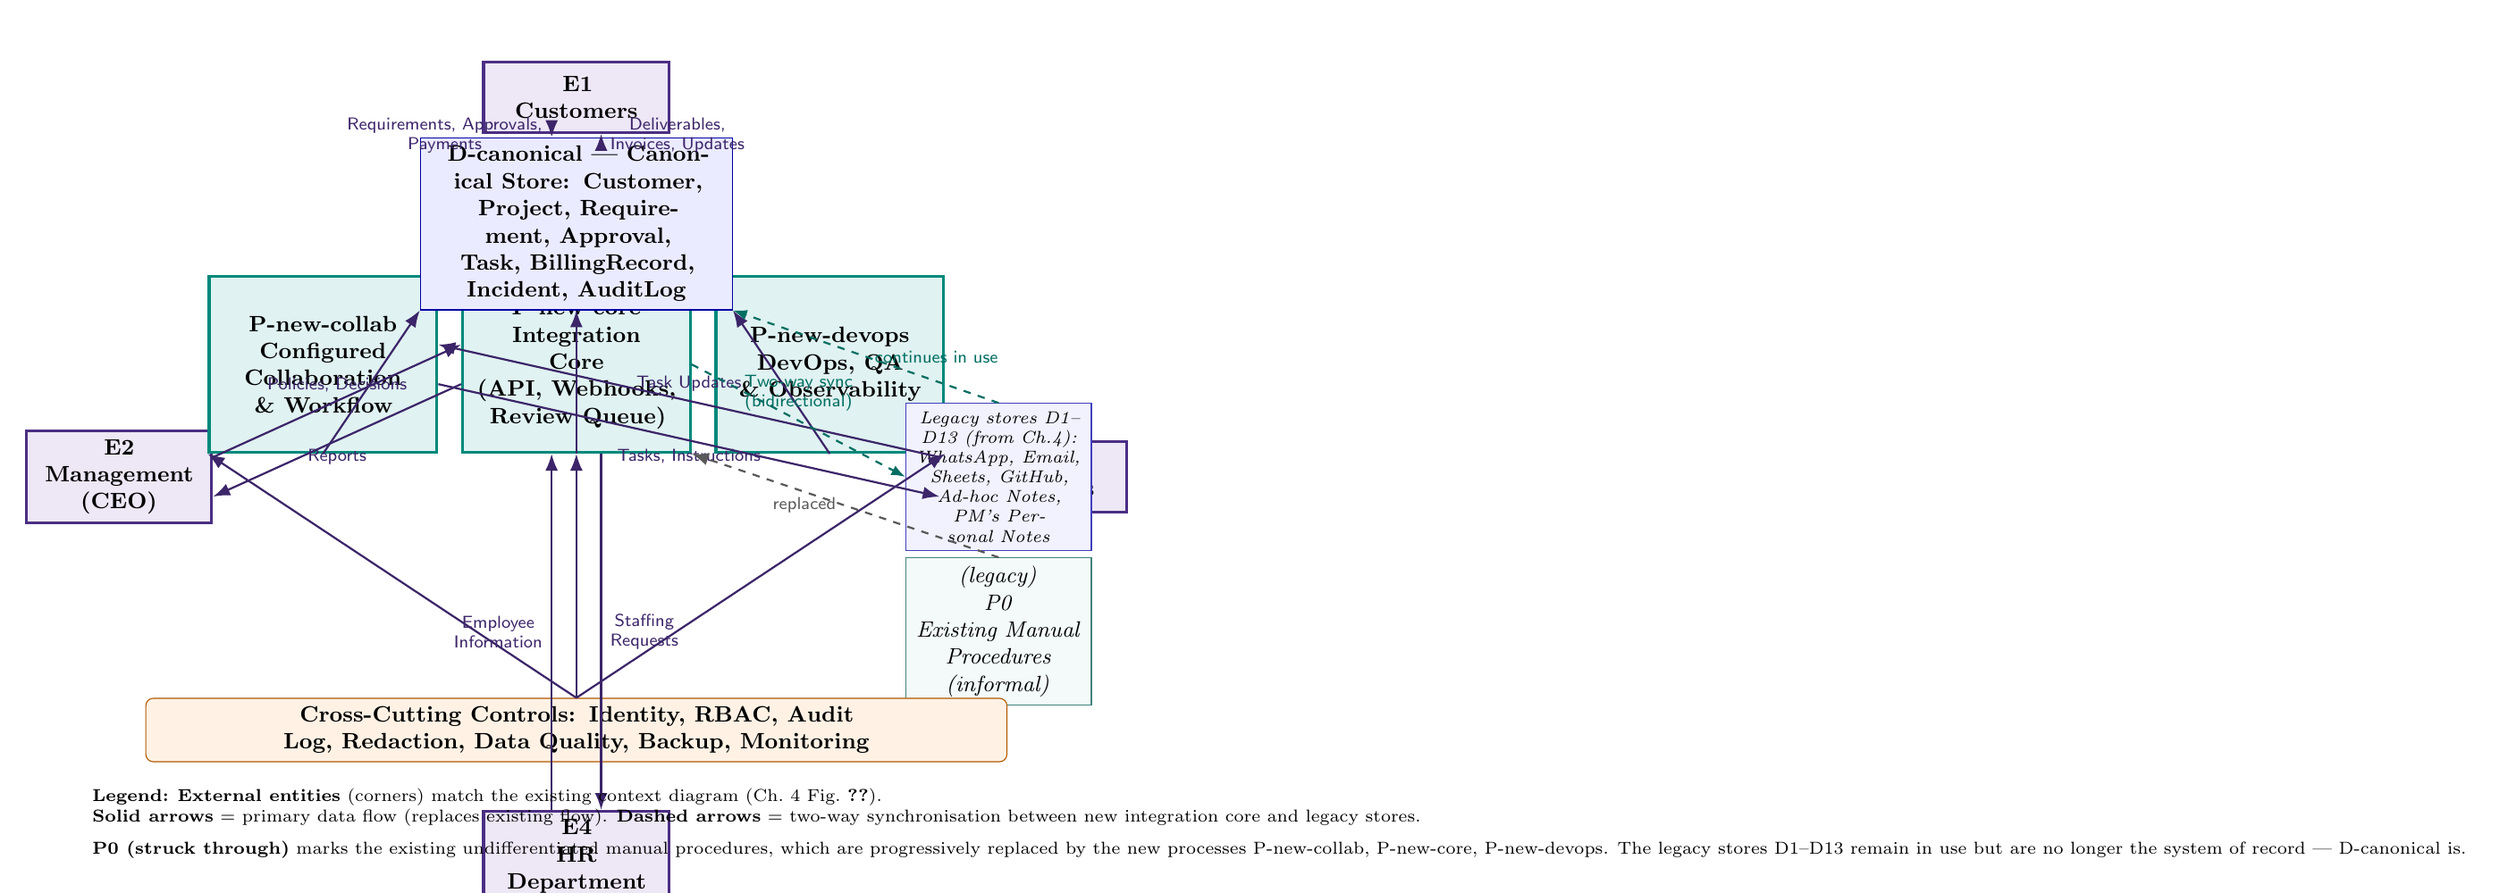
\begin{tikzpicture}[
    font=\small,
    entity/.style={draw=primary, fill=secondary, very thick, text width=2.4cm,
        align=center, minimum height=1.0cm, font=\small\bfseries},
    procnew/.style={draw=accent, fill=softteal, very thick, text width=3.0cm,
        align=center, minimum size=2.5cm, font=\small\bfseries},
    proclegacy/.style={draw=accent!50!gray, fill=softteal!40, text width=2.4cm,
        align=center, minimum size=2.0cm, font=\small\itshape},
    storenew/.style={draw=blue!65!black, fill=blue!8, text width=4.2cm,
        align=center, minimum height=1.0cm, font=\small\bfseries},
    storlegacy/.style={draw=blue!50!gray, fill=blue!5, text width=2.4cm,
        align=center, minimum height=0.85cm, font=\scriptsize\itshape},
    cross/.style={draw=orange!70!black, rounded corners=3pt, fill=orange!10,
        text width=12.0cm, align=center, minimum height=0.9cm,
        font=\small\bfseries},
    flow/.style={-{Latex[length=2.4mm]}, thick, color=primary!80!black},
    flowsync/.style={-{Latex[length=2.0mm]}, thick, dashed, color=accent!80!black},
    flab/.style={font=\scriptsize\sffamily, align=center}
]

% --- External entities (same as existing context diagram) ---
\node[entity] (cust) at (0,    5.4) {\textbf{E1}\\Customers};
\node[entity] (ceo)  at (-6.5, 0) {\textbf{E2}\\Management\\(CEO)};
\node[entity] (emp)  at (6.5,  0) {\textbf{E3}\\Employees};
\node[entity] (hr)   at (0,   -5.4) {\textbf{E4}\\HR\\Department};

% --- New system processes (replacing P0) ---
\node[procnew] (pcollab) at (-3.6, 1.6) {P-new-collab\\Configured\\Collaboration\\\& Workflow};
\node[procnew] (pcore)   at (0,    1.6) {P-new-core\\Integration\\Core\\(API, Webhooks,\\Review Queue)};
\node[procnew] (pdevops) at (3.6,  1.6) {P-new-devops\\DevOps, QA\\\& Observability};

% --- New canonical store ---
\node[storenew] (dcanon) at (0, 3.6) {D-canonical --- Canonical Store: Customer, Project,
    Requirement, Approval, Task, BillingRecord, Incident, AuditLog};

% --- Legacy stores (existing D1--D13) shown faded on the right ---
\node[storlegacy] (lstore) at (6.0, 0) {Legacy stores D1--D13 (from Ch.4):\\WhatsApp, Email,
    Sheets, GitHub, Ad-hoc Notes,\\PM's Personal Notes};
\node[proclegacy] (p0) at (6.0, -2.2) {(legacy)\\P0\\Existing Manual\\Procedures\\(informal)};

% --- Cross-cutting controls ---
\node[cross] (security) at (0, -3.6)
    {Cross-Cutting Controls: Identity, RBAC, Audit Log, Redaction, Data Quality, Backup, Monitoring};

% --- Customer flows (same as existing context diagram) ---
\draw[flow] ([xshift=-10pt]cust.south) -- ([xshift=-10pt]dcanon.north)
    node[flab, midway, left] {Requirements, Approvals,\\Payments};
\draw[flow] ([xshift=10pt]dcanon.north) -- ([xshift=10pt]cust.south)
    node[flab, midway, right] {Deliverables,\\Invoices, Updates};

% --- Management (CEO) flows ---
\draw[flow] ([yshift=8pt]ceo.east) -- ([yshift=8pt]pcore.west)
    node[flab, midway, above] {Policies, Decisions};
\draw[flow] ([yshift=-8pt]pcore.west) -- ([yshift=-8pt]ceo.east)
    node[flab, midway, below] {Reports};

% --- Employees flows ---
\draw[flow] ([yshift=8pt]emp.west) -- ([yshift=8pt]pcollab.east)
    node[flab, midway, above] {Task Updates};
\draw[flow] ([yshift=-8pt]pcollab.east) -- ([yshift=-8pt]emp.west)
    node[flab, midway, below] {Tasks, Instructions};

% --- HR flows ---
\draw[flow] ([xshift=-10pt]hr.north) -- ([xshift=-10pt]pcore.south)
    node[flab, midway, left] {Employee\\Information};
\draw[flow] ([xshift=10pt]pcore.south) -- ([xshift=10pt]hr.north)
    node[flab, midway, right] {Staffing\\Requests};

% --- Internal new-system flows ---
\draw[flow] (pcollab.south) -- (dcanon.south west);
\draw[flow] (pcore.south) -- (dcanon.south);
\draw[flow] (pdevops.south) -- (dcanon.south east);

% --- New system bridges legacy stores (sync) ---
\draw[flowsync] (pcore.east) -- node[flab, midway, above]{\scriptsize Two-way sync\\(bidirectional)} (lstore.west);
\draw[flowsync] (lstore.north) -- node[flab, midway, right]{\scriptsize continues in use} (dcanon.south east);

% --- Legacy process P0 fades to the new system (migration) ---
\draw[flow, dashed, color=gray!70!black] (p0.north) -- node[flab, midway, left]{\scriptsize replaced} (pcore.south east);

% --- Cross-cutting controls wrap the new architecture ---
\draw[flow] (security.north) -- (pcollab.south west);
\draw[flow] (security.north) -- (pcore.south);
\draw[flow] (security.north) -- (pdevops.south east);

% --- Legend ---
\node[anchor=west, font=\scriptsize, align=left] at (-7.0, -4.7) {%
    \textbf{Legend:} \textbf{External entities} (corners) match the existing context
    diagram (Ch.~4 Fig.~\ref{fig:dfd_context}).\\
    \textbf{Solid arrows} = primary data flow (replaces existing flow). \textbf{Dashed
    arrows} = two-way synchronisation between new integration core and legacy stores.};
\node[anchor=west, font=\scriptsize, align=left] at (-7.0, -5.3) {%
    \textbf{P0 (struck through)} marks the existing undifferentiated manual procedures,
    which are progressively replaced by the new processes P-new-collab, P-new-core,
    P-new-devops. The legacy stores D1--D13 remain in use but are no longer the
    system of record --- D-canonical is.};

\end{tikzpicture}%
}
\caption{Complete System DFD --- the recommended new system drawn on top of
the existing context diagram. External entities (E1--E4) are the same as
Chapter~4, Figure~\ref{fig:dfd_context}; the undifferentiated process P0 is
replaced by three new processes (P-new-collab, P-new-core, P-new-devops) and
one canonical store (D-canonical). The existing data stores D1--D13 remain in
use but are now bridged to the canonical store through the integration core.}
\label{fig:dfd-complete-system}
\end{figure}

\noindent The diagram makes three architectural decisions visible that are
not visible in the existing-state DFDs of Chapter~4.

\begin{itemize}[leftmargin=1.6em]
    \item \textbf{The new system has structure where P0 had none.} The
          existing context diagram collapses all operations into a single
          process P0, which is exactly the abstraction that hides the
          fragmentation problem. The new diagram breaks P0 into three
          explicit new processes --- collaboration, integration core, and
          DevOps --- so the reader can see which layer is responsible for
          what, and so the governance controls can be attached to the
          right layer.
    \item \textbf{Legacy stores D1--D13 are kept but demoted.} The
          existing tools (WhatsApp, Sheets, GitHub, email, etc.) do not
          disappear. They remain in use, but they are no longer the
          \emph{system of record} --- the canonical store D-canonical is. The
          dashed arrows show the two-way synchronisation between the
          integration core and each legacy store. This is the Configure
          strategy in picture form: keep the tools the team already uses,
          layer governance over them, do not replace them.
    \item \textbf{Cross-cutting controls wrap the new architecture.} The
          existing system has no equivalent to the cross-cutting controls
          block. In the new system, identity, RBAC, audit, redaction, data
          quality, backup, and monitoring are implemented once in the
          integration core and enforced across every other layer, which
          is the structural answer to Problems~2 (fragmentation) and~4
          (security).
\end{itemize}

\noindent The same architecture, drawn with the data flows that the new
system actually carries and the problems those flows address, is shown in
Figure~\ref{fig:dfd-problem-solving}. That figure makes explicit \emph{why}
each flow exists and \emph{which} of the five problems identified in
Chapter~1 it solves, so the design can be read as a direct response to the
analysis rather than as a generic target architecture.

\begin{figure}[H]
\centering
\resizebox{\textwidth}{!}{%
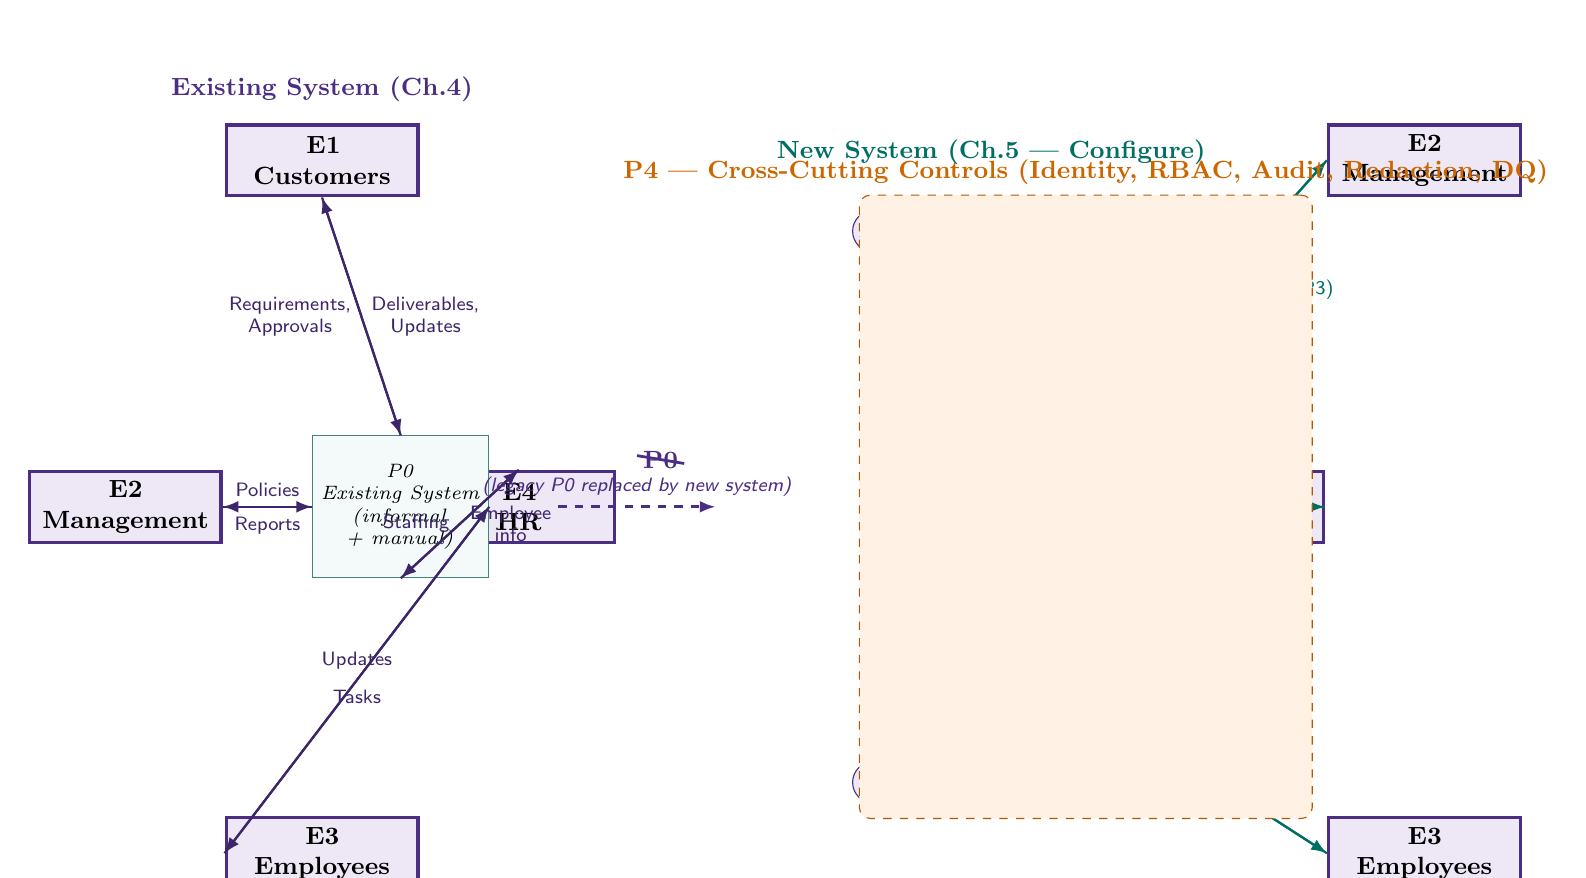
\begin{tikzpicture}[
    font=\small,
    entity/.style={draw=primary, fill=secondary, very thick, text width=2.2cm,
        align=center, minimum height=0.9cm, font=\small\bfseries},
    procold/.style={draw=accent!50!gray, fill=softteal!40, text width=2.0cm,
        align=center, minimum size=1.8cm, font=\scriptsize\itshape},
    procnew/.style={draw=accent, fill=softteal, text width=2.4cm,
        align=center, minimum size=2.2cm, font=\small\bfseries},
    ptag/.style={circle, draw=primary, fill=secondary, inner sep=1.2pt,
        font=\scriptsize\bfseries, minimum size=3.6mm},
    flow/.style={-{Latex[length=2.0mm]}, thick, color=primary!80!black},
    flownew/.style={-{Latex[length=2.0mm]}, thick, color=accent!80!black},
    flab/.style={font=\scriptsize\sffamily, align=center},
    fnlab/.style={font=\scriptsize\sffamily, align=center, color=accent!80!black}
]

% =====================================================
% EXISTING SYSTEM (LEFT HALF)  --- mirrors Ch.4 Fig. 4.1
% =====================================================

% External entities (left half)
\node[entity] (e1L) at (-7.0, 4.4) {\textbf{E1}\\Customers};
\node[entity] (e2L) at (-9.5, 0)  {\textbf{E2}\\Management};
\node[entity] (e3L) at (-7.0, -4.4) {\textbf{E3}\\Employees};
\node[entity] (e4L) at (-4.5, 0)  {\textbf{E4}\\HR};

% Existing process P0 (single undifferentiated, in the centre-left)
\node[procold] (p0) at (-6.0, 0) {P0\\Existing System\\(informal + manual)};

% Existing flow labels (mirroring Ch.4 Fig. 4.1)
\draw[flow] (e1L.south) -- node[flab, midway, left]{\scriptsize Requirements,\\Approvals} (p0.north);
\draw[flow] (p0.north) -- node[flab, midway, right]{\scriptsize Deliverables,\\Updates} (e1L.south);
\draw[flow] (e2L.east) -- node[flab, midway, above]{\scriptsize Policies} (p0.west);
\draw[flow] (p0.west) -- node[flab, midway, below]{\scriptsize Reports} (e2L.east);
\draw[flow] (e3L.west) -- node[flab, midway, above]{\scriptsize Updates} (p0.east);
\draw[flow] (p0.east) -- node[flab, midway, below]{\scriptsize Tasks} (e3L.west);
\draw[flow] (e4L.north) -- node[flab, midway, left]{\scriptsize Staffing} (p0.south);
\draw[flow] (p0.south) -- node[flab, midway, right]{\scriptsize Employee\\info} (e4L.north);

% Label for existing system
\node[font=\small\bfseries, color=primary] at (-7.0, 5.3) {Existing System (Ch.4)};

% =====================================================
% NEW SYSTEM (RIGHT HALF)  --- replaces P0
% =====================================================

% External entities (right half, same labels)
\node[entity] (e1R) at ( 4.5, 0)  {\textbf{E1}\\Customers};
\node[entity] (e2R) at ( 7.0, 4.4) {\textbf{E2}\\Management};
\node[entity] (e3R) at ( 7.0,-4.4) {\textbf{E3}\\Employees};
\node[entity] (e4R) at ( 4.5, 0)  {\textbf{E4}\\HR};

% New processes (replacing P0)
\node[procnew] (pcollab) at (1.5, 2.5) {P-new-collab\\Collaboration\\\& Workflow};
\node[procnew] (pcore)   at (1.5, 0)   {P-new-core\\Integration\\Core};
\node[procnew] (pdevops) at (1.5,-2.5) {P-new-devops\\DevOps,\\QA \& Obs.};

% Canonical store (between processes and external entities)
\node[procnew, text width=2.2cm, minimum size=1.0cm, fill=blue!8, draw=blue!65!black]
    (canon) at (4.0, 0) {D-canonical\\Customer,\\Project, Req,\\Task, \ldots};

% Problem badges near the new flows they address
\node[ptag] (p1) at (0.0,  3.5) {P1};
\node[ptag] (p2) at (3.5,  2.5) {P2};
\node[ptag] (p3) at (3.5,  0.0) {P3};
\node[ptag] (p4) at (3.5, -1.5) {P4};
\node[ptag] (p5) at (0.0, -3.5) {P5};

% New data flows (with problem tags implicitly on the diagrams below)
% e1 (Customers) -> P-new-collab (P1 fix: capture informal request)
\draw[flownew] (e1R.west) -- node[fnlab, midway, above]{\scriptsize Requirements\\(P1)} (pcollab.east);
\draw[flownew] (pcollab.east) -- node[fnlab, midway, below]{\scriptsize Deliverables} (e1R.west);
% e2 (Management) -> P-new-core (reports)
\draw[flownew] (e2R.west) -- node[fnlab, midway, left]{\scriptsize Policies} (pcore.north east);
\draw[flownew] (pcore.north east) -- node[fnlab, midway, right]{\scriptsize Reports (P3)} (e2R.west);
% e3 (Employees) -> P-new-devops (tasks/updates)
\draw[flownew] (e3R.west) -- node[fnlab, midway, below]{\scriptsize Updates} (pdevops.east);
\draw[flownew] (pdevops.east) -- node[fnlab, midway, above]{\scriptsize Tasks (P5)} (e3R.west);
% e4 (HR) -> P-new-core (employee info / staffing)
\draw[flownew] (e4R.east) -- node[fnlab, midway, above]{\scriptsize Employee\\info} (pcore.east);
\draw[flownew] (pcore.east) -- node[fnlab, midway, below]{\scriptsize Staffing} (e4R.east);

% New processes -> canonical store (P2, P3)
\draw[flownew] (pcollab.south) -- node[fnlab, midway, right]{\scriptsize Req/Approval\\(P2)} (canon.north west);
\draw[flownew] (pcore.east) -- node[fnlab, midway, above]{\scriptsize Sync\\(P3)} (canon.west);
\draw[flownew] (pdevops.north) -- node[fnlab, midway, right]{\scriptsize Release\\evidence (P2)} (canon.south west);

% Cross-cutting (P4) shown as a halo around the new system
\node[draw=orange!70!black, dashed, rounded corners, fill=orange!10,
    fit=(pcollab)(pcore)(pdevops)(canon), inner sep=10pt,
    label={[font=\small\bfseries, color=orange!80!black]above:{P4 --- Cross-Cutting Controls (Identity, RBAC, Audit, Redaction, DQ)}}] (halo) {};

% Label for new system
\node[font=\small\bfseries, color=accent!80!black] at (1.5, 4.5) {New System (Ch.5 --- Configure)};

% =====================================================
% MIGRATION ARROW (existing -> new)
% =====================================================
\draw[flow, dashed, very thick, color=primary] (-4.0, 0) -- node[flab, midway, above]{\textit{(legacy P0 replaced by new system)}} (-2.0, 0);

% "P0" struck-through effect, drawn manually as a node
\node[font=\small\bfseries, color=primary] at (-2.7, 0.6) {P0};
\draw[line width=1pt, color=primary] (-3.0, 0.65) -- (-2.4, 0.55);

\end{tikzpicture}%
}
\caption{Problem-Solving System DFD --- side-by-side comparison of the
existing system (left, from Chapter~4 Figure~\ref{fig:dfd_context}) and
the new system (right, replacing P0). External entities (E1--E4) are
the same in both halves. The problem badges (P1--P5) on the new flows
indicate which of the five Chapter~1 problems each flow addresses; the
full mapping is given in Table~\ref{tab:problem-flow-mapping}.}
\label{fig:dfd-problem-solving}
\end{figure}

\noindent Figure~\ref{fig:dfd-problem-solving} is read as a left-to-right
migration: the existing P0 on the left is replaced by the new processes
(P-new-collab, P-new-core, P-new-devops) and the new canonical store on
the right, with the same four external entities (E1--E4) and the same flow
categories as the existing context diagram. Every new flow is tagged with
the problem it addresses (P1--P5). The full mapping, including the specific
record or evidence that each new flow produces, is given in
Table~\ref{tab:problem-flow-mapping}.

\begin{table}[H]
\centering
\caption{Problem-to-Flow Mapping --- which new flow addresses which
problem, and the canonical record or evidence it produces.}
\label{tab:problem-flow-mapping}
\small
\renewcommand{\arraystretch}{1.30}
\setlength{\tabcolsep}{6pt}
\rowcolors{2}{roweven}{rowodd}
\begin{tabularx}{\textwidth}{>{\raggedright\arraybackslash}p{1.3cm}
                                >{\raggedright\arraybackslash}p{3.6cm}
                                >{\raggedright\arraybackslash}p{4.6cm}
                                >{\raggedright\arraybackslash}X}
\toprule
\textbf{Prob.} & \textbf{New Flow} & \textbf{Canonical Record / Evidence} & \textbf{What Changes for the User} \\
\midrule
P1 & Customer $\rightarrow$ Requirement Intake
      & \texttt{Requirements} (with \texttt{SourceMessage} provenance)
      & A chat message becomes a queryable record, not a forgotten thread. \\
P1 & PM $\rightarrow$ Approval Capture
      & \texttt{Approvals} (approver, decision, source, timestamp)
      & An informal "OK" in chat becomes evidence that the scope was approved. \\
P2 & All flows $\rightarrow$ Canonical Store (D-canonical)
      & One row per entity, one source of truth
      & A change in one tool automatically appears in the other connected tools. \\
P2 & Legacy stores D1--D13 $\leftrightarrow$ Integration Core
      & Two-way sync (dashed arrows)
      & Sheets, GitHub, chat, email keep working but are no longer the system of record. \\
P3 & Finance / Mgmt $\rightarrow$ Reporting
      & \texttt{BillingRecords} with \texttt{evidence\_bundle} JSON
      & Invoices are produced from a query, not from a manual reconciliation. \\
P3 & Integration Core $\rightarrow$ Data Quality service
      & \texttt{DataQuality} reports and exception queue
      & Inconsistencies between tools are surfaced, not hidden. \\
P4 & Cross-cutting controls (Identity, RBAC, Audit, Redaction)
      & \texttt{AuditLog}, RBAC roles, redacted fields
      & Every sensitive action is logged and access is governed by role, not by who happens to be in a chat. \\
P5 & Dev $\rightarrow$ Task \& Incident Workflow
      & \texttt{Tasks}, \texttt{Incidents} (template-driven, role-based)
      & Tasks are assigned through templates and capacity tags, not by a single coordinator. \\
P5 & Onboarding workflow (under P-new-collab)
      & \texttt{Users.capacity\_tag}, \texttt{Users.is\_mentor}
      & New hires are productive in weeks 1--2, not 4--6. \\
\bottomrule
\end{tabularx}
\end{table}

\noindent The five problems and the five architectural responses, in
summary, are:

\begin{itemize}[leftmargin=1.6em]
    \item \textbf{P1 (Fragmented Communication)} $\rightarrow$ Requirement
          Intake, Approval Capture, and SourceMessage provenance. Every
          informal decision becomes a canonical record.
    \item \textbf{P2 (System Fragmentation)} $\rightarrow$ Integration Core
          as single source of truth, with two-way sync to every connected
          tool. Legacy stores D1--D13 remain in use but are demoted.
    \item \textbf{P3 (Data Governance)} $\rightarrow$ Canonical schema with
          mandatory fields, validation, and a data-quality service that
          runs reconciliation and surfaces exceptions. Invoices are produced
          from a query, not from a manual reconciliation.
    \item \textbf{P4 (Security \& Access Control)} $\rightarrow$ Identity
          and RBAC, audit log, and redaction built in as cross-cutting
          services rather than as after-the-fact policies. Every sensitive
          action is logged; access is governed by role.
    \item \textbf{P5 (Scalability Bottlenecks)} $\rightarrow$ Templates,
          auto-assignment, role-based routing, and an onboarding workflow
          that does not depend on a single coordinator.
\end{itemize}

\noindent The diagram has four layers.

\begin{enumerate}[leftmargin=1.6em]
    \item \textbf{User layer (top)}: the five user groups interact primarily
          through the configured collaboration tool, with developers and QA
          additionally accessing the DevOps, QA, and observability stack for
          build, test, and release activities.
    \item \textbf{Functional layer (middle)}: the configured collaboration tool
          (e.g., Jira, ClickUp, Notion, or Linear) hosts the human-facing
          workflow for requirements, approvals, tasks, and onboarding. The
          DevOps, QA, and observability stack provides build, test, staging,
          release approval, monitoring, and incident management.
    \item \textbf{Integration core (bottom)}: a small canonical store with
          APIs and webhooks that records the canonical entities and exchanges
          data with both functional layers, ensuring that the collaboration
          tool, the DevOps stack, and any retained legacy system (Sheets, GitHub,
          email) stay synchronised around one source of truth.
    \item \textbf{Cross-cutting controls (foundation)}: identity, RBAC, audit,
          redaction, data quality, backup, and monitoring are implemented once
          in the integration core and enforced across every layer, so that
          security and governance are not bolted on after the fact.
\end{enumerate}

\noindent The three subsystem DFDs that follow (5.2.2, 5.2.3, 5.2.4) decompose
each of the three functional layers and the integration core, in turn, into the
sub-processes that each layer is responsible for.

% ----------------------------------------------------------------
\subsection{Integration Core Subsystem DFD}
\label{sec:dfd-integration-core}

The integration core is the foundation of the Configure strategy. It owns the
canonical record of the business entities (customer, project, requirement, approval,
task, billing record, incident, employee-capacity), provides the API and webhook
gateway through which the collaboration tool, the DevOps stack, and the retained
legacy systems exchange data, and implements the cross-cutting controls (identity,
RBAC, audit, redaction, data quality, backup, monitoring) that the rest of the
system relies on. The subsystem DFD in Figure~\ref{fig:dfd-integration-core} shows
the internal sub-processes of the integration core.

\begin{figure}[H]
\centering
\resizebox{0.95\textwidth}{!}{%
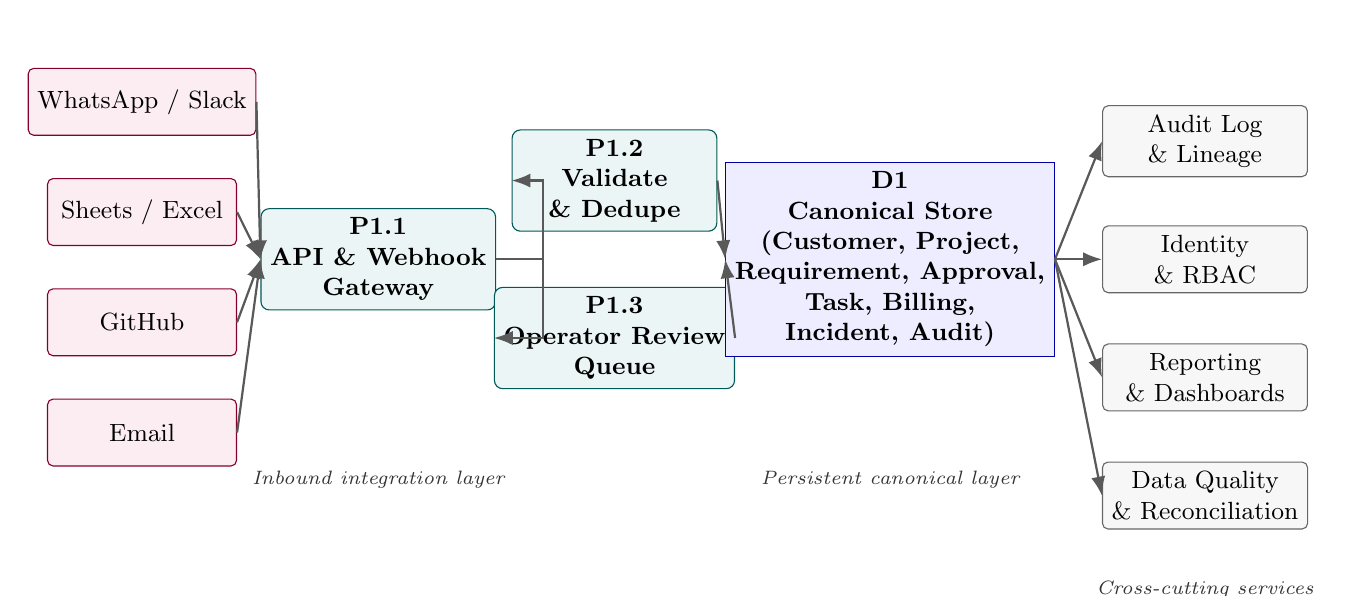
\begin{tikzpicture}[
    font=\small,
    ext/.style={draw=purple!70!black, rounded corners=2pt, fill=purple!7,
        minimum width=2.4cm, minimum height=.85cm, align=center},
    proc/.style={draw=teal!70!black, rounded corners=3pt, fill=teal!8,
        minimum width=2.6cm, minimum height=1.0cm, align=center, font=\small\bfseries},
    store/.style={draw=blue!65!black, fill=blue!7, minimum width=2.6cm,
        minimum height=1.0cm, align=center, font=\small\bfseries},
    service/.style={draw=black!60, rounded corners=2pt, fill=black!3,
        minimum width=2.6cm, minimum height=.85cm, align=center},
    arrow/.style={-{Latex[length=2.4mm]}, thick, draw=black!65}
]

% External connectors (left)
\node[ext] (wa) at (-4.0,3.0) {WhatsApp / Slack};
\node[ext] (sheet) at (-4.0,1.6) {Sheets / Excel};
\node[ext] (git) at (-4.0,0.2) {GitHub};
\node[ext] (email) at (-4.0,-1.2) {Email};

% Inbound gateway process
\node[proc] (gateway) at (-1.0,1.0) {P1.1\\API \& Webhook\\Gateway};

% Validation and dedupe
\node[proc] (validate) at (2.0,2.0) {P1.2\\Validate\\\& Dedupe};
\node[proc] (review) at (2.0,0.0) {P1.3\\Operator Review\\Queue};

% Canonical store
\node[store] (canonical) at (5.5,1.0) {D1\\Canonical Store\\(Customer, Project,\\Requirement, Approval,\\Task, Billing,\\Incident, Audit)};

% Outbound services (right)
\node[service] (audit) at (9.5,2.5) {Audit Log\\\& Lineage};
\node[service] (iam) at (9.5,1.0) {Identity\\\& RBAC};
\node[service] (dash) at (9.5,-0.5) {Reporting\\\& Dashboards};
\node[service] (dq) at (9.5,-2.0) {Data Quality\\\& Reconciliation};

% Flows from connectors into gateway
\foreach \n in {wa,sheet,git,email}{\draw[arrow] (\n.east) -- (gateway.west);}

% Gateway to validation / review
\draw[arrow] (gateway.east) -- ++(0.6,0) |- (validate.west);
\draw[arrow] (gateway.east) -- ++(0.6,0) |- (review.west);

% Validation / review into canonical
\draw[arrow] (validate.east) -- (canonical.west);
\draw[arrow] (review.east) -- (canonical.west);

% Cross-cutting services around canonical
\draw[arrow] (canonical.east) -- (audit.west);
\draw[arrow] (canonical.east) -- (iam.west);
\draw[arrow] (canonical.east) -- (dash.west);
\draw[arrow] (canonical.east) -- (dq.west);

% Background label
\node[font=\scriptsize\itshape, color=darkgray] at (-1.0,-1.8) {Inbound integration layer};
\node[font=\scriptsize\itshape, color=darkgray] at (5.5,-1.8) {Persistent canonical layer};
\node[font=\scriptsize\itshape, color=darkgray] at (9.5,-3.2) {Cross-cutting services};

\end{tikzpicture}%
}
\caption{Integration Core Subsystem DFD}
\label{fig:dfd-integration-core}
\end{figure}

\noindent The integration core is organised into three functional bands.

\begin{itemize}[leftmargin=1.6em]
    \item \textbf{Inbound integration layer (left band).} The gateway (P1.1)
          receives webhooks and scheduled imports from the retained legacy
          tools --- WhatsApp / Slack, Sheets / Excel, GitHub, and email ---
          and normalises them into candidate records. The validator (P1.2)
          applies the canonical schema, runs duplicate detection, and either
          persists the record or, when the match is ambiguous, escalates it
          to the operator review queue (P1.3).
    \item \textbf{Persistent canonical layer (centre).} The canonical store
          (D1) holds the authoritative record of every business entity, with
          provenance metadata that records the source tool, the operator who
          approved the record (if any), and the timestamp of each change. Audit
          lineage is derived from these provenance fields rather than from a
          separate system.
    \item \textbf{Cross-cutting services (right band).} The canonical store
          exposes a query and event API to four services: an audit log and
          lineage service, an identity and RBAC service, a reporting and
          dashboards service, and a data quality and reconciliation service.
          These services are the cross-cutting controls (Section~4.4) made
          concrete.
\end{itemize}

The review queue (P1.3) is the human-in-the-loop exception path. Its purpose is to
keep the system from forcing low-confidence records into the canonical store; it is
the operational expression of the "operator review" component from the high-level
architecture and is critical for the chat-approval capture workflow described in
the configured collaboration subsystem (5.2.3).

% ----------------------------------------------------------------
\subsection{Configured Collaboration \& Workflow Subsystem DFD}
\label{sec:dfd-collaboration}

The configured collaboration and workflow subsystem is where the human-facing work
of the system happens. It is built on a best-of-breed commercial tool (e.g., Jira,
ClickUp, Notion, or Linear) configured with templates, automation rules, and
approval flows that match NextStepBD's operational reality. The subsystem DFD in
Figure~\ref{fig:dfd-collaboration} shows the internal sub-processes and the flows
to and from the integration core.

\begin{figure}[H]
\centering
\resizebox{0.95\textwidth}{!}{%
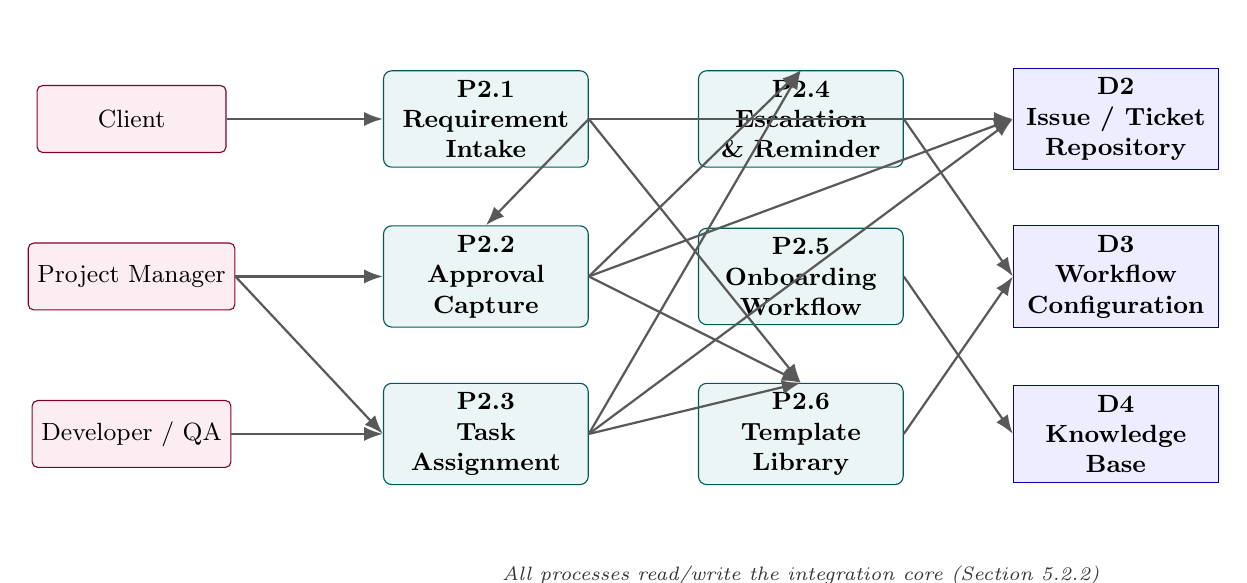
\begin{tikzpicture}[
    font=\small,
    actor/.style={draw=purple!70!black, rounded corners=2pt, fill=purple!7,
        minimum width=2.4cm, minimum height=.85cm, align=center},
    proc/.style={draw=teal!70!black, rounded corners=3pt, fill=teal!8,
        minimum width=2.6cm, minimum height=1.0cm, align=center, font=\small\bfseries},
    store/.style={draw=blue!65!black, fill=blue!7, minimum width=2.6cm,
        minimum height=1.0cm, align=center, font=\small\bfseries},
    arrow/.style={-{Latex[length=2.4mm]}, thick, draw=black!65}
]

% Actors (left)
\node[actor] (client) at (-4.5,2.6) {Client};
\node[actor] (pm) at (-4.5,0.6) {Project Manager};
\node[actor] (dev) at (-4.5,-1.4) {Developer / QA};

% Workflow processes (centre)
\node[proc] (intake) at (0.0,2.6) {P2.1\\Requirement\\Intake};
\node[proc] (approve) at (0.0,0.6) {P2.2\\Approval\\Capture};
\node[proc] (task) at (0.0,-1.4) {P2.3\\Task\\Assignment};
\node[proc] (escalate) at (4.0,2.6) {P2.4\\Escalation\\\& Reminder};
\node[proc] (onboard) at (4.0,0.6) {P2.5\\Onboarding\\Workflow};
\node[proc] (template) at (4.0,-1.4) {P2.6\\Template\\Library};

% Stores
\node[store] (issue) at (8.0,2.6) {D2\\Issue / Ticket\\Repository};
\node[store] (conf) at (8.0,0.6) {D3\\Workflow\\Configuration};
\node[store] (know) at (8.0,-1.4) {D4\\Knowledge\\Base};

% Cross-cutting link
\node[font=\scriptsize\itshape, color=darkgray, align=center] at (4.0,-3.2) {All processes read/write the integration core (Section 5.2.2)};

% Actor to process flows
\draw[arrow] (client.east) -- (intake.west);
\draw[arrow] (pm.east) -- (approve.west);
\draw[arrow] (pm.east) -- (task.west);
\draw[arrow] (dev.east) -- (task.west);

% Process internal flows
\draw[arrow] (intake.east) -- (approve.north);
\draw[arrow] (intake.east) -- (template.north);
\draw[arrow] (approve.east) -- (escalate.north);
\draw[arrow] (approve.east) -- (template.north);
\draw[arrow] (task.east) -- (escalate.north);
\draw[arrow] (task.east) -- (template.north);

% Process to store flows
\draw[arrow] (intake.east) -- (issue.west);
\draw[arrow] (approve.east) -- (issue.west);
\draw[arrow] (task.east) -- (issue.west);
\draw[arrow] (escalate.east) -- (conf.west);
\draw[arrow] (onboard.east) -- (know.west);
\draw[arrow] (template.east) -- (conf.west);

\end{tikzpicture}%
}
\caption{Configured Collaboration \& Workflow Subsystem DFD}
\label{fig:dfd-collaboration}
\end{figure}

\noindent The subsystem has six sub-processes organised in two columns.

\begin{itemize}[leftmargin=1.6em]
    \item \textbf{Left column --- the core request-to-task flow.}
          \begin{itemize}
              \item P2.1 \textbf{Requirement Intake}: a client or internal
                    user submits a requirement through a form (Section~5.4.1)
                    or a structured channel. The requirement is recorded in
                    the issue / ticket repository (D2) and a corresponding
                    canonical record is created in the integration core
                    (Section~5.2.2).
              \item P2.2 \textbf{Approval Capture}: an approval that happened
                    informally in chat or email is captured into the
                    workflow tool through a one-click confirmation, then
                    promoted into the canonical approval record. This is
                    the principal fix for Problem~1 (fragmented
                    communication).
              \item P2.3 \textbf{Task Assignment}: tasks are created from
                    requirements, linked to owners, and dispatched to
                    developers. Templates from the template library (P2.6)
                    are applied for routine task types.
          \end{itemize}
    \item \textbf{Right column --- the supporting processes.}
          \begin{itemize}
              \item P2.4 \textbf{Escalation \& Reminder}: automated
                    escalation timers, reminder rules, and role-based
                    notifications ensure that work items are not blocked
                    by a single absent stakeholder. The escalation policy is
                    stored in the workflow configuration (D3).
              \item P2.5 \textbf{Onboarding Workflow}: new hires are
                    onboarded through a structured workflow with checklists,
                    mentorship assignments, and a skills-tag capture that
                    feeds the integration core's employee-capacity record.
                    This is the principal fix for Problem~5 (scalability).
              \item P2.6 \textbf{Template Library}: a curated set of
                    templates for requirements, approvals, tasks, incidents,
                    and onboarding flows. Templates are the lever by which
                    process standardisation scales without adding per-team
                    customisation overhead.
          \end{itemize}
\end{itemize}

All six processes read and write the canonical store through the integration core
(5.2.2). The bidirectional connection is the structural reason why the
collaboration tool does not become yet another silo: every meaningful event in the
tool is captured as a canonical record, and every canonical record can be surfaced
back in the tool through a linked view.

% ----------------------------------------------------------------
\subsection{DevOps, QA \& Observability Subsystem DFD}
\label{sec:dfd-devops}

The DevOps, QA, and observability subsystem is responsible for the technical
delivery pipeline. It standardises build, test, staging, release, monitoring, and
incident management for the pilot projects, and it links deployment evidence back
to the canonical requirements and approvals in the integration core. The subsystem
DFD in Figure~\ref{fig:dfd-devops} shows the pipeline from code commit to
production, with the observability loop that closes it.

\begin{figure}[H]
\centering
\resizebox{0.95\textwidth}{!}{%
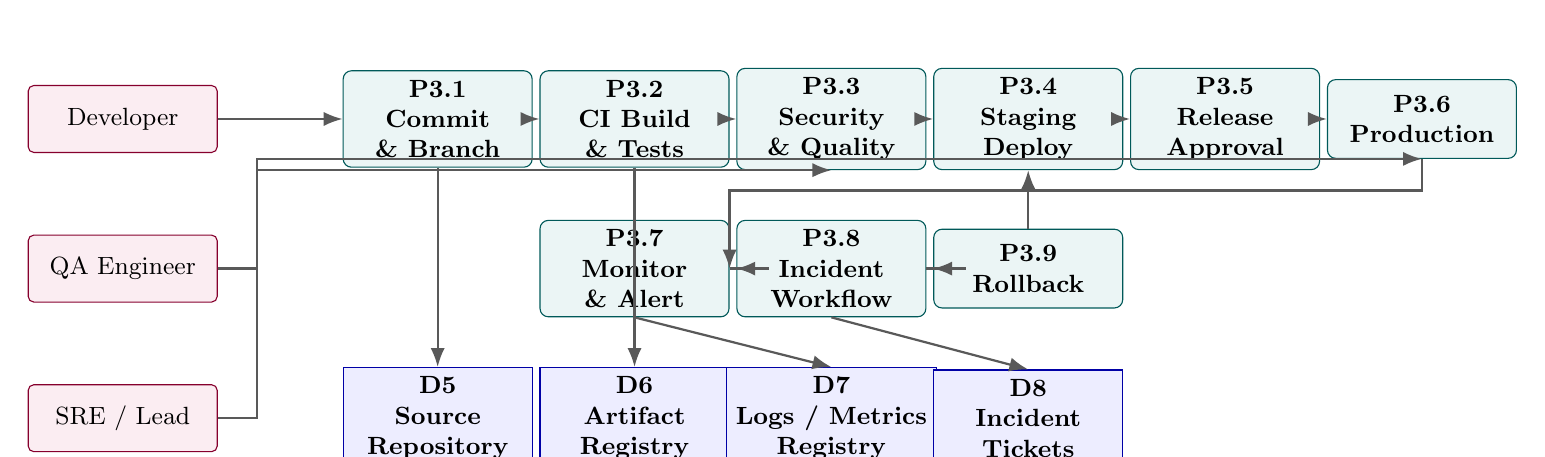
\begin{tikzpicture}[
    font=\small,
    actor/.style={draw=purple!70!black, rounded corners=2pt, fill=purple!7,
        minimum width=2.4cm, minimum height=.85cm, align=center},
    proc/.style={draw=teal!70!black, rounded corners=3pt, fill=teal!8,
        minimum width=2.4cm, minimum height=1.0cm, align=center, font=\small\bfseries},
    store/.style={draw=blue!65!black, fill=blue!7, minimum width=2.4cm,
        minimum height=1.0cm, align=center, font=\small\bfseries},
    arrow/.style={-{Latex[length=2.4mm]}, thick, draw=black!65}
]

% Actors
\node[actor] (dev) at (-3.5,0.5) {Developer};
\node[actor] (qa) at (-3.5,-1.4) {QA Engineer};
\node[actor] (sre) at (-3.5,-3.3) {SRE / Lead};

% Pipeline
\node[proc] (commit) at (0.5,0.5) {P3.1\\Commit\\\& Branch};
\node[proc] (ci) at (3.0,0.5) {P3.2\\CI Build\\\& Tests};
\node[proc] (security) at (5.5,0.5) {P3.3\\Security\\\& Quality};
\node[proc] (staging) at (8.0,0.5) {P3.4\\Staging\\Deploy};
\node[proc] (release) at (10.5,0.5) {P3.5\\Release\\Approval};
\node[proc] (prod) at (13.0,0.5) {P3.6\\Production};

% Observability layer
\node[proc] (monitor) at (3.0,-1.4) {P3.7\\Monitor\\\& Alert};
\node[proc] (incident) at (5.5,-1.4) {P3.8\\Incident\\Workflow};
\node[proc] (rollback) at (8.0,-1.4) {P3.9\\Rollback};

% Stores
\node[store] (repo) at (0.5,-3.3) {D5\\Source\\Repository};
\node[store] (art) at (3.0,-3.3) {D6\\Artifact\\Registry};
\node[store] (logs) at (5.5,-3.3) {D7\\Logs / Metrics\\Registry};
\node[store] (tickets) at (8.0,-3.3) {D8\\Incident\\Tickets};

% Main pipeline flow
\draw[arrow] (dev.east) -- (commit.west);
\draw[arrow] (commit) -- (ci);
\draw[arrow] (ci) -- (security);
\draw[arrow] (security) -- (staging);
\draw[arrow] (staging) -- (release);
\draw[arrow] (release) -- (prod);

% Cross-cutting loops
\draw[arrow] (prod.south) -- ++(0,-0.4) -| (monitor.east);
\draw[arrow] (monitor.east) -- ++(0.5,0) |- (incident.west);
\draw[arrow] (incident.east) -- ++(0.5,0) |- (rollback.west);
\draw[arrow] (rollback.north) -- ++(0,0.4) -| (staging.south);

% Stores
\draw[arrow] (commit.south) -- (repo.north);
\draw[arrow] (ci.south) -- (art.north);
\draw[arrow] (monitor.south) -- (logs.north);
\draw[arrow] (incident.south) -- (tickets.north);

% QA gate
\draw[arrow] (qa.east) -- ++(0.5,0) |- (security.south);
\draw[arrow] (sre.east) -- ++(0.5,0) |- (prod.south);

\end{tikzpicture}%
}
\caption{DevOps, QA, and Observability Subsystem DFD}
\label{fig:dfd-devops}
\end{figure}

\noindent The subsystem is a linear pipeline (top row) closed by an observability
loop (middle row) and supported by four stores (bottom row).

\begin{itemize}[leftmargin=1.6em]
    \item \textbf{Top row --- the delivery pipeline.}
          \begin{itemize}
              \item P3.1 \textbf{Commit \& Branch}: developer pushes code to
                    the source repository (D5) following the project's
                    branching policy.
              \item P3.2 \textbf{CI Build \& Tests}: continuous integration
                    runs the build, unit tests, integration tests, and
                    regression tests. Successful builds produce an
                    immutable artifact in the artifact registry (D6).
              \item P3.3 \textbf{Security \& Quality}: automated security
                    scanning, dependency checks, linting, and code-quality
                    gates run on every build. QA engineers review and
                    sign off the test report before staging.
              \item P3.4 \textbf{Staging Deploy}: the artifact is deployed
                    to a staging environment that mirrors production.
                    Smoke tests and integration tests run against staging.
              \item P3.5 \textbf{Release Approval}: a formal release
                    approval is recorded against the deployment, linked
                    to the requirement or task that drove the change. This
                    is where the canonical store receives a \emph{release
                    evidence} record.
              \item P3.6 \textbf{Production}: the artifact is deployed to
                    production with health checks in place.
          \end{itemize}
    \item \textbf{Middle row --- the observability loop.}
          \begin{itemize}
              \item P3.7 \textbf{Monitor \& Alert}: continuous monitoring of
                    logs, metrics, and uptime (D7) produces alerts on
                    service-level breaches.
              \item P3.8 \textbf{Incident Workflow}: an alert opens an
                    incident ticket (D8) in the collaboration tool, linked
                    to the affected requirement or task.
              \item P3.9 \textbf{Rollback}: an incident can trigger a
                    rollback to the previous production artifact.
          \end{itemize}
\end{itemize}

The observability loop closes back to the staging stage: when monitoring detects a
regression, the system can roll forward to a known-good artifact or roll back to
the previous one. The release approval (P3.5) is the operational moment at which
the canonical record of "what was deployed, by whom, against which requirement"
is created; that record is the evidence that the system can use for change
tracking, billing evidence, and audit.

% ----------------------------------------------------------------
\section{Database Design}
\label{sec:design-database}

The database design is the persistent foundation of the recommended system. It
specifies exactly how the canonical entities identified in Section~5.2.2 are
structured, constrained, and related, so that the data model is internally
consistent, supports the workflows of Section~5.2.3, and persists the release and
incident evidence created by Section~5.2.4.

The database architecture for the proposed system addresses five requirement
buckets that were identified through the root cause analysis and the comparative
feasibility evaluation:

\begin{itemize}[leftmargin=1.6em]
    \item \textbf{Canonical operational record.} Structured storage for
          customers, projects, requirements, approvals, and tasks, providing the
          authoritative record that the collaboration tool and the DevOps
          stack both read from and write to. This is the principal fix for
          Problems~2 (fragmentation) and~3 (data governance).
    \item \textbf{Billing and operational readiness.} Tables that connect
          approved scope and accepted deliverables to invoice preparation
          and supporting evidence, so that finance and operations can
          produce invoices without manual cross-referencing. This is the
          principal fix for the billing evidence gap that contributed to
          Problem~3.
    \item \textbf{Audit, security, and access.} Tables for the audit log, the
          user roster, and the role catalogue, with foreign-key linkage to
          every entity that an operator can touch. This is the principal
          fix for Problem~4 (security and access control).
    \item \textbf{Incident and capacity tracking.} Tables for incidents
          (post-deployment issues, support tickets) and employee-capacity
          tags (skills, current load, mentor status) that the workflow
          system and the DevOps system both depend on. This is the
          principal fix for Problem~5 (scalability).
    \item \textbf{System integration.} The SourceMessage table records
          inbound events from legacy tools (Sheets, GitHub, chat) with
          provenance, so that any record in the canonical store is
          traceable to its original source. Foreign-key relationships
          enforce referential integrity across the eight core tables.
\end{itemize}

All tables are designed to Third Normal Form (3NF) to eliminate update anomalies
and redundancy. Integrity constraints (NOT NULL, UNIQUE, CHECK, FOREIGN KEY) are
applied systematically. Indexing strategies prioritise the high-frequency query
patterns identified in the functional requirements --- in particular, the
approval lookup (P2.2 in Figure~\ref{fig:dfd-collaboration}) and the
requirement-to-task traversal (P2.3).

% ----------------------------------------------------------------
\subsection{ER Diagram}
\label{sec:design-er}

Figure~\ref{fig:er-diagram} shows the Entity-Relationship diagram for the eight
core tables of the canonical data model. Entities are shown as rectangles,
attributes as ovals, and relationships as connecting lines with cardinality
indicators. Foreign-key relationships are explicit, and the audit lineage is
modelled as a first-class relationship from every canonical entity to the
AuditLog table.

\begin{figure}[H]
\centering
\resizebox{0.95\textwidth}{!}{%
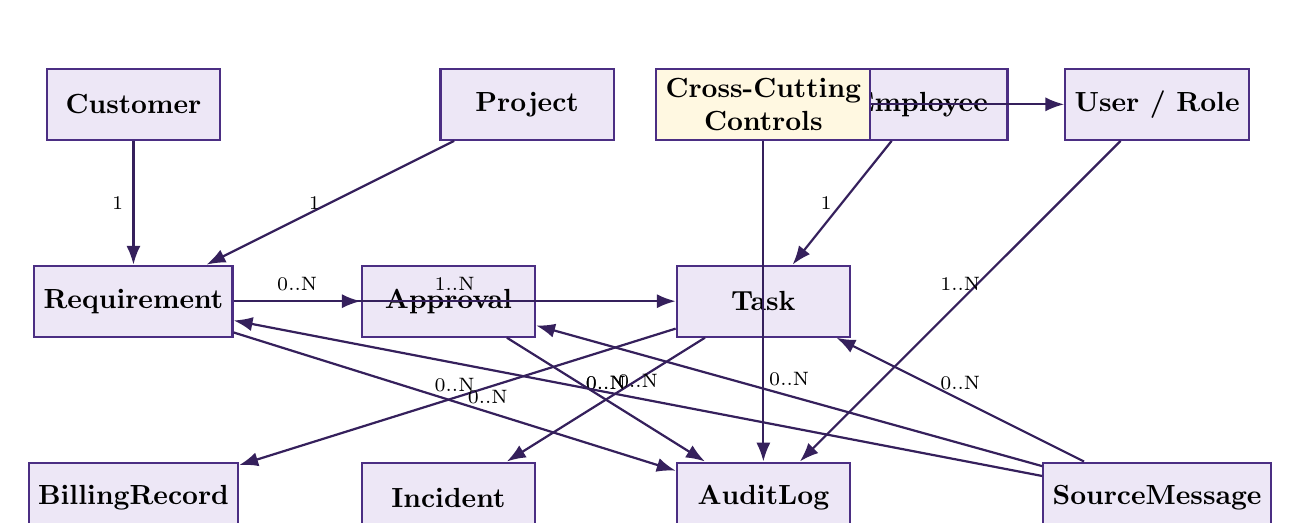
\begin{tikzpicture}[
    font=\small,
    entity/.style={draw=primary, fill=secondary, thick, minimum width=2.2cm,
        minimum height=0.9cm, align=center, font=\bfseries},
    rel/.style={draw=accent, thick, align=center, font=\scriptsize},
    arrow/.style={-{Latex[length=2.4mm]}, thick, draw=primary!70!black}
]

% Top row: Customer, Project
\node[entity] (customer) at (0,4) {Customer};
\node[entity] (project) at (5,4) {Project};
\node[entity] (employee) at (10,4) {Employee};
\node[entity] (user) at (13,4) {User / Role};

% Middle row: Requirement, Approval, Task
\node[entity] (requirement) at (0,1.5) {Requirement};
\node[entity] (approval) at (4,1.5) {Approval};
\node[entity] (task) at (8,1.5) {Task};

% Bottom row: Billing, Incident, AuditLog, SourceMessage
\node[entity] (billing) at (0,-1) {BillingRecord};
\node[entity] (incident) at (4,-1) {Incident};
\node[entity] (audit) at (8,-1) {AuditLog};
\node[entity] (source) at (13,-1) {SourceMessage};

% Cross-cutting center
\node[entity, fill=softcream] (xref) at (8,4) {\shortstack{Cross-Cutting\\Controls}};

% Relationships (top row -> middle row)
\draw[arrow] (customer) -- node[left, font=\scriptsize]{1} (requirement);
\draw[arrow] (project) -- node[left, font=\scriptsize]{1} (requirement);
\draw[arrow] (requirement) -- node[above, font=\scriptsize]{0..N} (approval);
\draw[arrow] (requirement) -- node[above, font=\scriptsize]{1..N} (task);
\draw[arrow] (employee) -- node[left, font=\scriptsize]{1} (task);
\draw[arrow] (user) -- node[above, font=\scriptsize]{1..N} (audit);

% Middle row -> bottom row
\draw[arrow] (task) -- node[right, font=\scriptsize]{0..N} (billing);
\draw[arrow] (task) -- node[above, font=\scriptsize]{0..N} (incident);
\draw[arrow] (approval) -- node[above, font=\scriptsize]{0..N} (audit);
\draw[arrow] (requirement) -- node[above, font=\scriptsize]{0..N} (audit);
\draw[arrow] (source) -- node[above, font=\scriptsize]{0..N} (requirement);
\draw[arrow] (source) -- node[above, font=\scriptsize]{0..N} (approval);
\draw[arrow] (source) -- node[above, font=\scriptsize]{0..N} (task);
\draw[arrow] (xref) -- (audit);
\draw[arrow] (xref) -- (user);

\end{tikzpicture}%
}
\caption{ER Diagram --- Canonical Data Model}
\label{fig:er-diagram}
\end{figure}

\noindent The cardinality of the principal relationships is:

\begin{itemize}[leftmargin=1.6em]
    \item \textbf{Customer} 1 --- N \textbf{Project} (a customer may have
          many projects, each project has exactly one customer).
    \item \textbf{Project} 1 --- N \textbf{Requirement} (a project has many
          requirements; a requirement belongs to one project).
    \item \textbf{Requirement} 1 --- N \textbf{Approval} (each requirement
          may have one or more approvals, including scope, sign-off, and
          delivery approvals).
    \item \textbf{Requirement} 1 --- N \textbf{Task} (a requirement is
          decomposed into one or more tasks).
    \item \textbf{Employee} 1 --- N \textbf{Task} (an employee can be
          assigned many tasks; a task is assigned to one employee at a
          time).
    \item \textbf{Task} 0..N --- 1 \textbf{BillingRecord} (a task may be
          billable; a billing record aggregates one or more tasks into an
          invoice line).
    \item \textbf{Task} 0..N --- 1 \textbf{Incident} (a task or release may
          spawn an incident).
    \item \textbf{User} 1 --- N \textbf{AuditLog} (every audit record
          identifies a user actor).
    \item \textbf{SourceMessage} 0..N --- 1 \textbf{Requirement / Approval /
          Task} (a record may be traceable back to a source event).
\end{itemize}

The audit log is treated as a first-class entity, not as a side-effect of
operational tables. Every change to a canonical entity produces a row in
AuditLog with the actor, the timestamp, the before-image, and the after-image.
This means a regulator or auditor can answer "who changed this record, when,
and from what source" with a single SQL query, which is a substantial
improvement over the present state (Problem~4).

% ----------------------------------------------------------------
\subsection{Database Tables and Data Specifications}
\label{sec:design-tables}

The eight most operationally critical tables are specified below. The column
format is: field name, key type (PK = primary key, FK = foreign key, UQ =
unique), data type, size / constraint, and a one-line description. Each table
also carries a row-count estimate and an index note at the end of the
specification, since indexing strategy is a non-trivial part of the design
even though the column details are the primary deliverable.

\subsubsection{Users Table}
\label{tab:users}

The Users table is the master record of every individual who interacts with the
system, including internal employees and external client contacts. It is the
authoritative source of identity for the audit log, the assignment record, and
the approval record.

\begin{table}[H]
\centering
\caption{Users Table: Data Types and Specifications}
\small
\renewcommand{\arraystretch}{1.30}
\setlength{\tabcolsep}{6pt}
\rowcolors{2}{roweven}{rowodd}
\begin{tabularx}{\textwidth}{>{\raggedright\arraybackslash}p{2.6cm}
                                >{\centering\arraybackslash}p{1.4cm}
                                >{\raggedright\arraybackslash}p{2.2cm}
                                >{\raggedright\arraybackslash}p{3.4cm}
                                >{\raggedright\arraybackslash}X}
\rowcolor{headerbg}
\multicolumn{1}{>{\columncolor{headerbg}\raggedright\arraybackslash}p{2.6cm}}{\textcolor{headertx}{\textbf{Field Name}}} &
\multicolumn{1}{>{\columncolor{headerbg}\centering\arraybackslash}p{1.4cm}}{\textcolor{headertx}{\textbf{Key}}} &
\multicolumn{1}{>{\columncolor{headerbg}\raggedright\arraybackslash}p{2.2cm}}{\textcolor{headertx}{\textbf{Data Type}}} &
\multicolumn{1}{>{\columncolor{headerbg}\raggedright\arraybackslash}p{3.4cm}}{\textcolor{headertx}{\textbf{Size / Constraint}}} &
\multicolumn{1}{>{\columncolor{headerbg}\raggedright\arraybackslash}X}{\textcolor{headertx}{\textbf{Description}}} \\
\midrule
user\_id           & \keyfmt{PK} & \dtype{INT}          & \dsize{NOT NULL, AUTO\_INCREMENT}   & Unique user identifier \\
full\_name         & \keyfmt{}   & \dtype{VARCHAR}      & \dsize{NOT NULL, 120}               & Display name \\
email              & \keyfmt{UQ} & \dtype{VARCHAR}      & \dsize{NOT NULL, 180}               & Login and notification address \\
role               & \keyfmt{}   & \dtype{ENUM}         & \dsize{NOT NULL}                    & CEO, PM, DEV, QA, FIN, OPS, HR, CLIENT, ADMIN \\
external\_id       & \keyfmt{}   & \dtype{VARCHAR}      & \dsize{120}                         & SSO provider subject (Keycloak, Google) \\
capacity\_tag      & \keyfmt{}   & \dtype{VARCHAR}      & \dsize{40}                          & Skill tag for auto-assignment (e.g., backend-go) \\
is\_mentor         & \keyfmt{}   & \dtype{BOOLEAN}      & \dsize{NOT NULL, DEFAULT FALSE}     & Onboarding mentor flag \\
created\_at        & \keyfmt{}   & \dtype{TIMESTAMP}    & \dsize{NOT NULL, DEFAULT NOW}       & Account creation time \\
last\_login\_at     & \keyfmt{}   & \dtype{TIMESTAMP}    & \dsize{NULL}                        & Last successful authentication \\
\bottomrule
\end{tabularx}
\end{table}

\noindent \emph{Indexes}: PK on \texttt{user\_id}; UQ on \texttt{email};
INDEX on \texttt{role} (for role-based dashboards); INDEX on
\texttt{capacity\_tag} (for capacity-based auto-assignment).

% ----------------------------------------------------------------
\subsubsection{Customers Table}
\label{tab:customers}

The Customers table is the master record of every client organisation that
NextStepBD serves. It is the parent of the Project table and the source of
billing references.

\begin{table}[H]
\centering
\caption{Customers Table: Data Types and Specifications}
\small
\renewcommand{\arraystretch}{1.30}
\setlength{\tabcolsep}{6pt}
\rowcolors{2}{roweven}{rowodd}
\begin{tabularx}{\textwidth}{>{\raggedright\arraybackslash}p{2.6cm}
                                >{\raggedright\arraybackslash}p{1.4cm}
                                >{\raggedright\arraybackslash}p{2.2cm}
                                >{\raggedright\arraybackslash}p{3.4cm}
                                >{\raggedright\arraybackslash}X}
\rowcolor{headerbg}
\multicolumn{1}{>{\columncolor{headerbg}\raggedright\arraybackslash}p{2.6cm}}{\textcolor{headertx}{\textbf{Field Name}}} &
\multicolumn{1}{>{\columncolor{headerbg}\centering\arraybackslash}p{1.4cm}}{\textcolor{headertx}{\textbf{Key}}} &
\multicolumn{1}{>{\columncolor{headerbg}\raggedright\arraybackslash}p{2.2cm}}{\textcolor{headertx}{\textbf{Data Type}}} &
\multicolumn{1}{>{\columncolor{headerbg}\raggedright\arraybackslash}p{3.4cm}}{\textcolor{headertx}{\textbf{Size / Constraint}}} &
\multicolumn{1}{>{\columncolor{headerbg}\raggedright\arraybackslash}X}{\textcolor{headertx}{\textbf{Description}}} \\
\midrule
customer\_id & \keyfmt{PK} & \dtype{INT} & \dsize{NOT NULL, AUTO\_INCREMENT} & Unique customer identifier \\
name & \keyfmt{} & \dtype{VARCHAR} & \dsize{NOT NULL, 200} & Customer organisation name \\
primary\_contact & \keyfmt{FK} & \dtype{INT} & \dsize{NOT NULL, REFERENCES Users} & Primary contact user \\
billing\_email & \keyfmt{} & \dtype{VARCHAR} & \dsize{180} & Address for invoice delivery \\
billing\_address & \keyfmt{} & \dtype{TEXT} & \dsize{NULL} & Postal address for invoicing \\
tax\_id & \keyfmt{} & \dtype{VARCHAR} & \dsize{40} & VAT / tax identifier \\
contract\_type & \keyfmt{} & \dtype{ENUM} & \dsize{NOT NULL} & PROJECT, RETAINER, MIXED \\
status & \keyfmt{} & \dtype{ENUM} & \dsize{NOT NULL} & ACTIVE, PAUSED, CLOSED \\
created\_at & \keyfmt{} & \dtype{TIMESTAMP} & \dsize{NOT NULL, DEFAULT NOW} & Onboarding date \\
updated\_at & \keyfmt{} & \dtype{TIMESTAMP} & \dsize{NOT NULL, ON UPDATE NOW} & Last canonical change \\
\bottomrule
\end{tabularx}
\end{table}

\noindent \emph{Indexes}: PK on \texttt{customer\_id}; UQ on \texttt{name} +
\texttt{billing\_email} (preventing duplicate onboarding); FK index on
\texttt{primary\_contact}; INDEX on \texttt{status} (for active-client
dashboards).

% ----------------------------------------------------------------
\subsubsection{Projects Table}
\label{tab:projects}

The Projects table is the parent of every requirement, approval, and task. Each
project has exactly one customer and may have one or more team members drawn
from the Users table.

\begin{table}[H]
\centering
\caption{Projects Table: Data Types and Specifications}
\small
\renewcommand{\arraystretch}{1.30}
\setlength{\tabcolsep}{6pt}
\rowcolors{2}{roweven}{rowodd}
\begin{tabularx}{\textwidth}{>{\raggedright\arraybackslash}p{2.6cm}
                                >{\raggedright\arraybackslash}p{1.4cm}
                                >{\raggedright\arraybackslash}p{2.2cm}
                                >{\raggedright\arraybackslash}p{3.4cm}
                                >{\raggedright\arraybackslash}X}
\rowcolor{headerbg}
\multicolumn{1}{>{\columncolor{headerbg}\raggedright\arraybackslash}p{2.6cm}}{\textcolor{headertx}{\textbf{Field Name}}} &
\multicolumn{1}{>{\columncolor{headerbg}\centering\arraybackslash}p{1.4cm}}{\textcolor{headertx}{\textbf{Key}}} &
\multicolumn{1}{>{\columncolor{headerbg}\raggedright\arraybackslash}p{2.2cm}}{\textcolor{headertx}{\textbf{Data Type}}} &
\multicolumn{1}{>{\columncolor{headerbg}\raggedright\arraybackslash}p{3.4cm}}{\textcolor{headertx}{\textbf{Size / Constraint}}} &
\multicolumn{1}{>{\columncolor{headerbg}\raggedright\arraybackslash}X}{\textcolor{headertx}{\textbf{Description}}} \\
\midrule
project\_id & \keyfmt{PK} & \dtype{INT} & \dsize{NOT NULL, AUTO\_INCREMENT} & Unique project identifier \\
customer\_id & \keyfmt{FK} & \dtype{INT} & \dsize{NOT NULL, REFERENCES Customers} & Owning customer \\
name & \keyfmt{} & \dtype{VARCHAR} & \dsize{NOT NULL, 200} & Project name \\
code & \keyfmt{UQ} & \dtype{VARCHAR} & \dsize{NOT NULL, 20} & Short code, e.g., AC-2026-07 \\
status & \keyfmt{} & \dtype{ENUM} & \dsize{NOT NULL} & PLANNED, ACTIVE, PAUSED, CLOSED \\
pm\_user\_id & \keyfmt{FK} & \dtype{INT} & \dsize{NOT NULL, REFERENCES Users} & Project manager \\
start\_date & \keyfmt{} & \dtype{DATE} & \dsize{NULL} & Project start \\
end\_date & \keyfmt{} & \dtype{DATE} & \dsize{NULL} & Projected end \\
sheet\_source\_id & \keyfmt{} & \dtype{VARCHAR} & \dsize{60} & External Google Sheet ID, if applicable \\
created\_at & \keyfmt{} & \dtype{TIMESTAMP} & \dsize{NOT NULL, DEFAULT NOW} & Record creation \\
\bottomrule
\end{tabularx}
\end{table}

\noindent \emph{Indexes}: PK on \texttt{project\_id}; UQ on \texttt{code}; FK
index on \texttt{customer\_id}; FK index on \texttt{pm\_user\_id}; INDEX on
\texttt{status} (for portfolio dashboards).

% ----------------------------------------------------------------
\subsubsection{Requirements Table}
\label{tab:requirements}

The Requirements table is the canonical record of every feature, change, or
scope item the customer has agreed to. Each requirement has one or more
approvals and is decomposed into one or more tasks. This is the principal
fix for Problem~1 (fragmented communication), because the requirement is the
first place where an informal decision is promoted into a structured record.

\begin{table}[H]
\centering
\caption{Requirements Table: Data Types and Specifications}
\small
\renewcommand{\arraystretch}{1.30}
\setlength{\tabcolsep}{6pt}
\rowcolors{2}{roweven}{rowodd}
\begin{tabularx}{\textwidth}{>{\raggedright\arraybackslash}p{2.6cm}
                                >{\raggedright\arraybackslash}p{1.4cm}
                                >{\raggedright\arraybackslash}p{2.2cm}
                                >{\raggedright\arraybackslash}p{3.4cm}
                                >{\raggedright\arraybackslash}X}
\rowcolor{headerbg}
\multicolumn{1}{>{\columncolor{headerbg}\raggedright\arraybackslash}p{2.6cm}}{\textcolor{headertx}{\textbf{Field Name}}} &
\multicolumn{1}{>{\columncolor{headerbg}\centering\arraybackslash}p{1.4cm}}{\textcolor{headertx}{\textbf{Key}}} &
\multicolumn{1}{>{\columncolor{headerbg}\raggedright\arraybackslash}p{2.2cm}}{\textcolor{headertx}{\textbf{Data Type}}} &
\multicolumn{1}{>{\columncolor{headerbg}\raggedright\arraybackslash}p{3.4cm}}{\textcolor{headertx}{\textbf{Size / Constraint}}} &
\multicolumn{1}{>{\columncolor{headerbg}\raggedright\arraybackslash}X}{\textcolor{headertx}{\textbf{Description}}} \\
\midrule
requirement\_id & \keyfmt{PK} & \dtype{INT} & \dsize{NOT NULL, AUTO\_INCREMENT} & Unique requirement identifier \\
project\_id & \keyfmt{FK} & \dtype{INT} & \dsize{NOT NULL, REFERENCES Projects} & Owning project \\
title & \keyfmt{} & \dtype{VARCHAR} & \dsize{NOT NULL, 200} & Short description \\
description & \keyfmt{} & \dtype{TEXT} & \dsize{NOT NULL} & Full requirement text \\
source\_id & \keyfmt{FK} & \dtype{INT} & \dsize{NULL, REFERENCES SourceMessages} & Provenance to original chat / email / sheet row \\
priority & \keyfmt{} & \dtype{ENUM} & \dsize{NOT NULL} & LOW, MEDIUM, HIGH, CRITICAL \\
status & \keyfmt{} & \dtype{ENUM} & \dsize{NOT NULL} & DRAFT, APPROVED, IN\_PROGRESS, DONE, WITHDRAWN \\
acceptance\_criteria & \keyfmt{} & \dtype{TEXT} & \dsize{NULL} & Definition-of-done for QA \\
created\_by & \keyfmt{FK} & \dtype{INT} & \dsize{NOT NULL, REFERENCES Users} & User who created the record \\
created\_at & \keyfmt{} & \dtype{TIMESTAMP} & \dsize{NOT NULL, DEFAULT NOW} & Record creation \\
updated\_at & \keyfmt{} & \dtype{TIMESTAMP} & \dsize{NOT NULL, ON UPDATE NOW} & Last canonical change \\
\bottomrule
\end{tabularx}
\end{table}

\noindent \emph{Indexes}: PK on \texttt{requirement\_id}; FK index on
\texttt{project\_id}; FK index on \texttt{source\_id}; INDEX on
\texttt{status} (for in-flight requirement dashboards); INDEX on
\texttt{priority} (for backlog prioritisation).

% ----------------------------------------------------------------
\subsubsection{Approvals Table}
\label{tab:approvals}

The Approvals table is the canonical record of every approval decision, no
matter where the decision was originally communicated. It is the structural
answer to Problem~1: a binding approval is never "in a chat" or "in an email"
--- it is always here, with the actor, the timestamp, the artefact approved,
and the source from which the decision was captured.

\begin{table}[H]
\centering
\caption{Approvals Table: Data Types and Specifications}
\small
\renewcommand{\arraystretch}{1.30}
\setlength{\tabcolsep}{6pt}
\rowcolors{2}{roweven}{rowodd}
\begin{tabularx}{\textwidth}{>{\raggedright\arraybackslash}p{2.6cm}
                                >{\raggedright\arraybackslash}p{1.4cm}
                                >{\raggedright\arraybackslash}p{2.2cm}
                                >{\raggedright\arraybackslash}p{3.4cm}
                                >{\raggedright\arraybackslash}X}
\rowcolor{headerbg}
\multicolumn{1}{>{\columncolor{headerbg}\raggedright\arraybackslash}p{2.6cm}}{\textcolor{headertx}{\textbf{Field Name}}} &
\multicolumn{1}{>{\columncolor{headerbg}\centering\arraybackslash}p{1.4cm}}{\textcolor{headertx}{\textbf{Key}}} &
\multicolumn{1}{>{\columncolor{headerbg}\raggedright\arraybackslash}p{2.2cm}}{\textcolor{headertx}{\textbf{Data Type}}} &
\multicolumn{1}{>{\columncolor{headerbg}\raggedright\arraybackslash}p{3.4cm}}{\textcolor{headertx}{\textbf{Size / Constraint}}} &
\multicolumn{1}{>{\columncolor{headerbg}\raggedright\arraybackslash}X}{\textcolor{headertx}{\textbf{Description}}} \\
\midrule
approval\_id & \keyfmt{PK} & \dtype{INT} & \dsize{NOT NULL, AUTO\_INCREMENT} & Unique approval identifier \\
requirement\_id & \keyfmt{FK} & \dtype{INT} & \dsize{NOT NULL, REFERENCES Requirements} & Requirement being approved \\
approver\_user\_id & \keyfmt{FK} & \dtype{INT} & \dsize{NOT NULL, REFERENCES Users} & Person who approved \\
decision & \keyfmt{} & \dtype{ENUM} & \dsize{NOT NULL} & APPROVED, REJECTED, CONDITIONAL \\
conditions & \keyfmt{} & \dtype{TEXT} & \dsize{NULL} & Free-text conditions attached to a CONDITIONAL approval \\
source\_id & \keyfmt{FK} & \dtype{INT} & \dsize{NULL, REFERENCES SourceMessages} & Provenance to the chat / email / form where it was captured \\
captured\_via & \keyfmt{} & \dtype{ENUM} & \dsize{NOT NULL} & ONE\_CLICK\_CONFIRM, OPERATOR\_REVIEW, FORM, INTEGRATION \\
captured\_at & \keyfmt{} & \dtype{TIMESTAMP} & \dsize{NOT NULL, DEFAULT NOW} & Capture timestamp \\
approved\_at & \keyfmt{} & \dtype{TIMESTAMP} & \dsize{NULL} & Original decision timestamp, if different from capture \\
\bottomrule
\end{tabularx}
\end{table}

\noindent \emph{Indexes}: PK on \texttt{approval\_id}; FK index on
\texttt{requirement\_id}; FK index on \texttt{approver\_user\_id}; FK index on
\texttt{source\_id}; INDEX on \texttt{captured\_via} (for review of which
approvals were operator-verified vs. self-captured).

% ----------------------------------------------------------------
\subsubsection{Tasks Table}
\label{tab:tasks}

The Tasks table is the operational unit of work. Each task is created from a
requirement (or, in incident-driven cases, from an Incident) and assigned to an
employee. Tasks are the principal entity consumed by the DevOps, QA, and
observability subsystem (Section~5.2.4).

\begin{table}[H]
\centering
\caption{Tasks Table: Data Types and Specifications}
\small
\renewcommand{\arraystretch}{1.30}
\setlength{\tabcolsep}{6pt}
\rowcolors{2}{roweven}{rowodd}
\begin{tabularx}{\textwidth}{>{\raggedright\arraybackslash}p{2.6cm}
                                >{\raggedright\arraybackslash}p{1.4cm}
                                >{\raggedright\arraybackslash}p{2.2cm}
                                >{\raggedright\arraybackslash}p{3.4cm}
                                >{\raggedright\arraybackslash}X}
\rowcolor{headerbg}
\multicolumn{1}{>{\columncolor{headerbg}\raggedright\arraybackslash}p{2.6cm}}{\textcolor{headertx}{\textbf{Field Name}}} &
\multicolumn{1}{>{\columncolor{headerbg}\centering\arraybackslash}p{1.4cm}}{\textcolor{headertx}{\textbf{Key}}} &
\multicolumn{1}{>{\columncolor{headerbg}\raggedright\arraybackslash}p{2.2cm}}{\textcolor{headertx}{\textbf{Data Type}}} &
\multicolumn{1}{>{\columncolor{headerbg}\raggedright\arraybackslash}p{3.4cm}}{\textcolor{headertx}{\textbf{Size / Constraint}}} &
\multicolumn{1}{>{\columncolor{headerbg}\raggedright\arraybackslash}X}{\textcolor{headertx}{\textbf{Description}}} \\
\midrule
task\_id & \keyfmt{PK} & \dtype{INT} & \dsize{NOT NULL, AUTO\_INCREMENT} & Unique task identifier \\
requirement\_id & \keyfmt{FK} & \dtype{INT} & \dsize{NOT NULL, REFERENCES Requirements} & Originating requirement \\
assignee\_user\_id & \keyfmt{FK} & \dtype{INT} & \dsize{NULL, REFERENCES Users} & Currently assigned employee \\
title & \keyfmt{} & \dtype{VARCHAR} & \dsize{NOT NULL, 200} & Short description \\
status & \keyfmt{} & \dtype{ENUM} & \dsize{NOT NULL} & TODO, IN\_PROGRESS, IN\_REVIEW, DONE, BLOCKED \\
priority & \keyfmt{} & \dtype{ENUM} & \dsize{NOT NULL} & LOW, MEDIUM, HIGH, CRITICAL \\
estimate\_hours & \keyfmt{} & \dtype{DECIMAL(5,1)} & \dsize{NULL} & Initial estimate \\
logged\_hours & \keyfmt{} & \dtype{DECIMAL(5,1)} & \dsize{NULL, DEFAULT 0.0} & Time logged against this task \\
is\_billable & \keyfmt{} & \dtype{BOOLEAN} & \dsize{NOT NULL, DEFAULT TRUE} & Whether this task contributes to billing \\
external\_issue\_id & \keyfmt{} & \dtype{VARCHAR} & \dsize{60} & ID in the configured collaboration tool \\
github\_pr\_url & \keyfmt{} & \dtype{VARCHAR} & \dsize{300} & Linked pull request URL, if any \\
release\_id & \keyfmt{FK} & \dtype{INT} & \dsize{NULL, REFERENCES AuditLog} & Linked release approval (when DONE) \\
created\_at & \keyfmt{} & \dtype{TIMESTAMP} & \dsize{NOT NULL, DEFAULT NOW} & Record creation \\
updated\_at & \keyfmt{} & \dtype{TIMESTAMP} & \dsize{NOT NULL, ON UPDATE NOW} & Last canonical change \\
\bottomrule
\end{tabularx}
\end{table}

\noindent \emph{Indexes}: PK on \texttt{task\_id}; FK index on
\texttt{requirement\_id}; FK index on \texttt{assignee\_user\_id}; UQ on
\texttt{external\_issue\_id} (to prevent duplicate sync from the collaboration
tool); INDEX on \texttt{status} (for Kanban-style dashboards); INDEX on
\texttt{is\_billable} (for billing extraction).

% ----------------------------------------------------------------
\subsubsection{BillingRecords Table}
\label{tab:billing}

The BillingRecords table aggregates approved scope and accepted deliverables
into invoice-ready records. Each row is the canonical evidence supporting a
billing line; finance and operations consume this table to produce invoices
without manual cross-referencing. This is the principal fix for the
billing-evidence gap in Problem~3.

\begin{table}[H]
\centering
\caption{BillingRecords Table: Data Types and Specifications}
\small
\renewcommand{\arraystretch}{1.30}
\setlength{\tabcolsep}{6pt}
\rowcolors{2}{roweven}{rowodd}
\begin{tabularx}{\textwidth}{>{\raggedright\arraybackslash}p{2.6cm}
                                >{\raggedright\arraybackslash}p{1.4cm}
                                >{\raggedright\arraybackslash}p{2.2cm}
                                >{\raggedright\arraybackslash}p{3.4cm}
                                >{\raggedright\arraybackslash}X}
\rowcolor{headerbg}
\multicolumn{1}{>{\columncolor{headerbg}\raggedright\arraybackslash}p{2.6cm}}{\textcolor{headertx}{\textbf{Field Name}}} &
\multicolumn{1}{>{\columncolor{headerbg}\centering\arraybackslash}p{1.4cm}}{\textcolor{headertx}{\textbf{Key}}} &
\multicolumn{1}{>{\columncolor{headerbg}\raggedright\arraybackslash}p{2.2cm}}{\textcolor{headertx}{\textbf{Data Type}}} &
\multicolumn{1}{>{\columncolor{headerbg}\raggedright\arraybackslash}p{3.4cm}}{\textcolor{headertx}{\textbf{Size / Constraint}}} &
\multicolumn{1}{>{\columncolor{headerbg}\raggedright\arraybackslash}X}{\textcolor{headertx}{\textbf{Description}}} \\
\midrule
billing\_id & \keyfmt{PK} & \dtype{INT} & \dsize{NOT NULL, AUTO\_INCREMENT} & Unique billing record identifier \\
project\_id & \keyfmt{FK} & \dtype{INT} & \dsize{NOT NULL, REFERENCES Projects} & Project being billed \\
invoice\_number & \keyfmt{UQ} & \dtype{VARCHAR} & \dsize{40} & Issued invoice number, NULL until invoiced \\
period\_start & \keyfmt{} & \dtype{DATE} & \dsize{NOT NULL} & Billing period start \\
period\_end & \keyfmt{} & \dtype{DATE} & \dsize{NOT NULL} & Billing period end \\
total\_amount & \keyfmt{} & \dtype{DECIMAL(12,2)} & \dsize{NOT NULL} & Total amount in BDT \\
currency & \keyfmt{} & \dtype{CHAR(3)} & \dsize{NOT NULL, DEFAULT 'BDT'} & Currency code \\
status & \keyfmt{} & \dtype{ENUM} & \dsize{NOT NULL} & DRAFT, SENT, PAID, OVERDUE \\
evidence\_bundle & \keyfmt{} & \dtype{JSON} & \dsize{NOT NULL} & Linked approval\_ids, task\_ids, release\_ids for audit \\
issued\_at & \keyfmt{} & \dtype{TIMESTAMP} & \dsize{NULL} & Time invoice was sent \\
paid\_at & \keyfmt{} & \dtype{TIMESTAMP} & \dsize{NULL} & Time payment was received \\
created\_at & \keyfmt{} & \dtype{TIMESTAMP} & \dsize{NOT NULL, DEFAULT NOW} & Record creation \\
\bottomrule
\end{tabularx}
\end{table}

\noindent \emph{Indexes}: PK on \texttt{billing\_id}; UQ on
\texttt{invoice\_number}; FK index on \texttt{project\_id}; INDEX on
\texttt{status} (for accounts-receivable ageing); INDEX on
\texttt{period\_start} (for periodic extraction).

The \texttt{evidence\_bundle} JSON column is the structural device that makes
billing auditable. It stores an array of the approval, task, and release IDs
that justify the line, so a regulator or auditor can reconstruct the chain of
evidence for any invoice with a single query, without re-reading chat
transcripts.

% ----------------------------------------------------------------
\subsubsection{AuditLog Table}
\label{tab:auditlog}

The AuditLog table is the canonical record of every change to a canonical
entity. It is the structural answer to Problem~4: every sensitive action is
logged with the actor, the timestamp, the before-image, and the after-image,
and the log is searchable, exportable, and retained per the policy in
Section~4.4 (auditability target: 100\% coverage of changes to canonical
records).

\begin{table}[H]
\centering
\caption{AuditLog Table: Data Types and Specifications}
\small
\renewcommand{\arraystretch}{1.30}
\setlength{\tabcolsep}{6pt}
\rowcolors{2}{roweven}{rowodd}
\begin{tabularx}{\textwidth}{>{\raggedright\arraybackslash}p{2.6cm}
                                >{\raggedright\arraybackslash}p{1.4cm}
                                >{\raggedright\arraybackslash}p{2.2cm}
                                >{\raggedright\arraybackslash}p{3.4cm}
                                >{\raggedright\arraybackslash}X}
\rowcolor{headerbg}
\multicolumn{1}{>{\columncolor{headerbg}\raggedright\arraybackslash}p{2.6cm}}{\textcolor{headertx}{\textbf{Field Name}}} &
\multicolumn{1}{>{\columncolor{headerbg}\centering\arraybackslash}p{1.4cm}}{\textcolor{headertx}{\textbf{Key}}} &
\multicolumn{1}{>{\columncolor{headerbg}\raggedright\arraybackslash}p{2.2cm}}{\textcolor{headertx}{\textbf{Data Type}}} &
\multicolumn{1}{>{\columncolor{headerbg}\raggedright\arraybackslash}p{3.4cm}}{\textcolor{headertx}{\textbf{Size / Constraint}}} &
\multicolumn{1}{>{\columncolor{headerbg}\raggedright\arraybackslash}X}{\textcolor{headertx}{\textbf{Description}}} \\
\midrule
audit\_id & \keyfmt{PK} & \dtype{BIGINT} & \dsize{NOT NULL, AUTO\_INCREMENT} & Monotonically increasing audit identifier \\
actor\_user\_id & \keyfmt{FK} & \dtype{INT} & \dsize{NOT NULL, REFERENCES Users} & Who performed the change \\
entity\_type & \keyfmt{} & \dtype{ENUM} & \dsize{NOT NULL} & CUSTOMER, PROJECT, REQUIREMENT, APPROVAL, TASK, BILLING, INCIDENT \\
entity\_id & \keyfmt{} & \dtype{INT} & \dsize{NOT NULL} & Primary key of the affected record \\
action & \keyfmt{} & \dtype{ENUM} & \dsize{NOT NULL} & CREATE, UPDATE, DELETE, EXPORT, VIEW, APPROVE, REJECT \\
before\_json & \keyfmt{} & \dtype{JSON} & \dsize{NULL} & Snapshot of the record before the change \\
after\_json & \keyfmt{} & \dtype{JSON} & \dsize{NULL} & Snapshot of the record after the change \\
ip\_address & \keyfmt{} & \dtype{VARCHAR} & \dsize{45} & Source IP for the change \\
user\_agent & \keyfmt{} & \dtype{VARCHAR} & \dsize{200} & Browser / client identifier \\
occurred\_at & \keyfmt{} & \dtype{TIMESTAMP} & \dsize{NOT NULL, DEFAULT NOW} & Event timestamp \\
\bottomrule
\end{tabularx}
\end{table}

\noindent \emph{Indexes}: PK on \texttt{audit\_id}; FK index on
\texttt{actor\_user\_id}; INDEX on \texttt{(entity\_type, entity\_id)} (for
"show me the history of this record"); INDEX on \texttt{occurred\_at} (for
time-range queries); INDEX on \texttt{action} (for compliance reports).

Because AuditLog is append-only and never updated, it is safe to retain
indefinitely and to expose to the data quality service for completeness
checks. A record that should be in AuditLog and is not is, by definition, a
data-integrity bug.

% ----------------------------------------------------------------
\subsubsection{Incidents Table}
\label{tab:incidents}

The Incidents table records post-deployment issues and support tickets. Each
incident is linked to the task or release that produced it (or to the
requirement that was affected), and is the operational entry point for the
DevOps, QA, and observability subsystem's incident workflow (P3.8 in
Figure~\ref{fig:dfd-devops}).

\begin{table}[H]
\centering
\caption{Incidents Table: Data Types and Specifications}
\small
\renewcommand{\arraystretch}{1.30}
\setlength{\tabcolsep}{6pt}
\rowcolors{2}{roweven}{rowodd}
\begin{tabularx}{\textwidth}{>{\raggedright\arraybackslash}p{2.6cm}
                                >{\raggedright\arraybackslash}p{1.4cm}
                                >{\raggedright\arraybackslash}p{2.2cm}
                                >{\raggedright\arraybackslash}p{3.4cm}
                                >{\raggedright\arraybackslash}X}
\rowcolor{headerbg}
\multicolumn{1}{>{\columncolor{headerbg}\raggedright\arraybackslash}p{2.6cm}}{\textcolor{headertx}{\textbf{Field Name}}} &
\multicolumn{1}{>{\columncolor{headerbg}\centering\arraybackslash}p{1.4cm}}{\textcolor{headertx}{\textbf{Key}}} &
\multicolumn{1}{>{\columncolor{headerbg}\raggedright\arraybackslash}p{2.2cm}}{\textcolor{headertx}{\textbf{Data Type}}} &
\multicolumn{1}{>{\columncolor{headerbg}\raggedright\arraybackslash}p{3.4cm}}{\textcolor{headertx}{\textbf{Size / Constraint}}} &
\multicolumn{1}{>{\columncolor{headerbg}\raggedright\arraybackslash}X}{\textcolor{headertx}{\textbf{Description}}} \\
\midrule
incident\_id & \keyfmt{PK} & \dtype{INT} & \dsize{NOT NULL, AUTO\_INCREMENT} & Unique incident identifier \\
title & \keyfmt{} & \dtype{VARCHAR} & \dsize{NOT NULL, 200} & Short description \\
severity & \keyfmt{} & \dtype{ENUM} & \dsize{NOT NULL} & P1, P2, P3, P4 \\
status & \keyfmt{} & \dtype{ENUM} & \dsize{NOT NULL} & OPEN, IN\_PROGRESS, RESOLVED, CLOSED \\
linked\_task\_id & \keyfmt{FK} & \dtype{INT} & \dsize{NULL, REFERENCES Tasks} & Originating task, if known \\
linked\_requirement\_id & \keyfmt{FK} & \dtype{INT} & \dsize{NULL, REFERENCES Requirements} & Affected requirement, if known \\
reporter\_user\_id & \keyfmt{FK} & \dtype{INT} & \dsize{NOT NULL, REFERENCES Users} & Who reported the incident \\
assignee\_user\_id & \keyfmt{FK} & \dtype{INT} & \dsize{NULL, REFERENCES Users} & On-call engineer currently assigned \\
root\_cause & \keyfmt{} & \dtype{TEXT} & \dsize{NULL} & Post-mortem summary when resolved \\
resolved\_at & \keyfmt{} & \dtype{TIMESTAMP} & \dsize{NULL} & Resolution timestamp \\
created\_at & \keyfmt{} & \dtype{TIMESTAMP} & \dsize{NOT NULL, DEFAULT NOW} & Report time \\
\bottomrule
\end{tabularx}
\end{table}

\noindent \emph{Indexes}: PK on \texttt{incident\_id}; FK index on
\texttt{linked\_task\_id}; FK index on \texttt{linked\_requirement\_id}; FK
index on \texttt{reporter\_user\_id}; FK index on \texttt{assignee\_user\_id};
INDEX on \texttt{severity} (for P1 dashboards); INDEX on
\texttt{(status, severity)} (for triage views).

% ----------------------------------------------------------------
\subsubsection{SourceMessage Table}
\label{tab:sourcemessage}

The SourceMessage table records every inbound event from a legacy system
(Sheets, GitHub, chat, email) that has been processed by the integration
core's gateway (P1.1 in Figure~\ref{fig:dfd-integration-core}). It is the
structural reason why the canonical record has provenance: every Requirements,
Approvals, or Tasks row that was created from a legacy source points back
to a SourceMessage row that records exactly what was received, when, and from
where.

\begin{table}[H]
\centering
\caption{SourceMessage Table: Data Types and Specifications}
\small
\renewcommand{\arraystretch}{1.30}
\setlength{\tabcolsep}{6pt}
\rowcolors{2}{roweven}{rowodd}
\begin{tabularx}{\textwidth}{>{\raggedright\arraybackslash}p{2.6cm}
                                >{\raggedright\arraybackslash}p{1.4cm}
                                >{\raggedright\arraybackslash}p{2.2cm}
                                >{\raggedright\arraybackslash}p{3.4cm}
                                >{\raggedright\arraybackslash}X}
\rowcolor{headerbg}
\multicolumn{1}{>{\columncolor{headerbg}\raggedright\arraybackslash}p{2.6cm}}{\textcolor{headertx}{\textbf{Field Name}}} &
\multicolumn{1}{>{\columncolor{headerbg}\centering\arraybackslash}p{1.4cm}}{\textcolor{headertx}{\textbf{Key}}} &
\multicolumn{1}{>{\columncolor{headerbg}\raggedright\arraybackslash}p{2.2cm}}{\textcolor{headertx}{\textbf{Data Type}}} &
\multicolumn{1}{>{\columncolor{headerbg}\raggedright\arraybackslash}p{3.4cm}}{\textcolor{headertx}{\textbf{Size / Constraint}}} &
\multicolumn{1}{>{\columncolor{headerbg}\raggedright\arraybackslash}X}{\textcolor{headertx}{\textbf{Description}}} \\
\midrule
source\_id & \keyfmt{PK} & \dtype{BIGINT} & \dsize{NOT NULL, AUTO\_INCREMENT} & Unique inbound event identifier \\
source\_type & \keyfmt{} & \dtype{ENUM} & \dsize{NOT NULL} & WHATSAPP, SLACK, EMAIL, SHEETS, GITHUB, FORM \\
source\_ref & \keyfmt{} & \dtype{VARCHAR} & \dsize{200} & External identifier (message ID, sheet row, PR number) \\
raw\_text & \keyfmt{} & \dtype{TEXT} & \dsize{NULL} & Original payload, redacted for PII if needed \\
parsed\_json & \keyfmt{} & \dtype{JSON} & \dsize{NULL} & Structured extraction by the validator (P1.2) \\
confidence & \keyfmt{} & \dtype{DECIMAL(3,2)} & \dsize{NULL} & Extraction confidence, 0.00--1.00 \\
mapped\_entity & \keyfmt{} & \dtype{ENUM} & \dsize{NULL} & REQUIREMENT, APPROVAL, TASK, INCIDENT (if recognised) \\
mapped\_entity\_id & \keyfmt{} & \dtype{INT} & \dsize{NULL} & FK to the resulting canonical row, if created \\
needs\_review & \keyfmt{} & \dtype{BOOLEAN} & \dsize{NOT NULL, DEFAULT FALSE} & Routed to operator review queue (P1.3) \\
received\_at & \keyfmt{} & \dtype{TIMESTAMP} & \dsize{NOT NULL, DEFAULT NOW} & Inbound timestamp from the source \\
processed\_at & \keyfmt{} & \dtype{TIMESTAMP} & \dsize{NULL} & When the validator (P1.2) finished extraction \\
\bottomrule
\end{tabularx}
\end{table}

\noindent \emph{Indexes}: PK on \texttt{source\_id}; INDEX on
\texttt{source\_type}; INDEX on \texttt{(source\_type, source\_ref)} (for
duplicate detection on re-sync); INDEX on \texttt{needs\_review} (for
operator queue dashboard); INDEX on \texttt{received\_at}.

% ----------------------------------------------------------------
\subsection{Table-to-Process Cross-Reference}
\label{sec:design-tables-xref}

The eight table specifications above are the operational deliverable of
Section~5.3, but they only become useful when the reader can see which process
writes to which table. Table~\ref{tab:tables-xref} provides that cross-reference
at a glance.

\begin{table}[H]
\centering
\caption{Cross-Reference: Tables to DFD Processes}
\label{tab:tables-xref}
\small
\renewcommand{\arraystretch}{1.18}
\begin{tabularx}{\textwidth}{>{\raggedright\arraybackslash}p{3.4cm}
                                >{\raggedright\arraybackslash}p{4.6cm}
                                >{\raggedright\arraybackslash}p{4.0cm}
                                >{\raggedright\arraybackslash}X}
\toprule
\textbf{Table} & \textbf{Primary Writer} & \textbf{Primary Reader} & \textbf{Primary Use} \\
\midrule
Users                 & Identity service            & All                       & Login, role-based access, capacity assignment \\
Customers             & CRM connector / form         & All                       & Customer master record \\
Projects              & PM workflow (P2.1)          & PMs, finance, management  & Project master record, portfolio view \\
Requirements          & Intake form (P2.1)          & PMs, developers, QA       & Work decomposition, acceptance criteria \\
Approvals             & Approval capture (P2.2)     & Finance, QA, PMs          & Authoritative approval evidence \\
Tasks                 & Task assignment (P2.3)      & Developers, QA, finance   & Operational work, billing extraction \\
BillingRecords        & Billing extraction (job)    & Finance, clients          & Invoice generation, evidence bundle \\
AuditLog              & All services                & Security, management, regulators & Compliance, change history, investigation \\
Incidents             & QA / on-call (P3.8)         & QA, PMs, SRE              & Defect and support tracking \\
SourceMessage         & Gateway (P1.1)              & All (transitively)        & Provenance for legacy-sourced records \\
\bottomrule
\end{tabularx}
\end{table}

% ----------------------------------------------------------------
\section{Form Design}
\label{sec:design-forms}

The form design section specifies the user interface layer for the five
operational forms that NextStepBD staff and clients use to enter data into
the system. Each form is purpose-calibrated to its user role and to the
process it feeds, and follows a consistent internal pattern: purpose, user
role, input fields, validation rules, and integration with the corresponding
database table and DFD process node. All forms are accessible through a
unified web-based staff portal and through a lightweight client portal for
external client users.

The five forms together cover the most important data entry touchpoints in
the recommended system:

\begin{enumerate}[leftmargin=1.6em]
    \item \textbf{Client Requirement Intake Form} --- the principal entry
          point for new requirements from clients.
    \item \textbf{Approval Capture Form} --- the structural answer to
          Problem~1 (fragmented communication); turns an approval that
          happened in chat or email into a canonical record.
    \item \textbf{Task Status / Change Request Form} --- used by
          developers and PMs to update a task, change scope, or record
          completion.
    \item \textbf{Incident Report Form} --- used by developers and QA to
          report a post-deployment issue.
    \item \textbf{Billing Evidence Form} --- used by finance to attach
          task and approval references to a billing period.
\end{enumerate}

% ----------------------------------------------------------------
\subsection{Client Requirement Intake Form}
\label{sec:form-intake}

\textbf{Purpose.} The Client Requirement Intake Form is the principal entry
point for new requirements from clients. It is used by account leads, project
managers, and (for client-portal self-service) by client users themselves.
The form turns a free-text client request into a structured Requirement
record (Section~\ref{tab:requirements}) and a linked draft issue in the
configured collaboration tool.

\textbf{User role.} Account lead, project manager, or client user (via the
client portal).

\textbf{Input fields.}

\begin{table}[H]
\centering
\caption{Client Requirement Intake Form: Input Fields}
\small
\renewcommand{\arraystretch}{1.30}
\setlength{\tabcolsep}{6pt}
\rowcolors{2}{roweven}{rowodd}
\begin{tabularx}{\textwidth}{>{\raggedright\arraybackslash}p{3.6cm}
                                >{\raggedright\arraybackslash}p{1.6cm}
                                >{\raggedright\arraybackslash}p{2.4cm}
                                >{\raggedright\arraybackslash}X}
\toprule
\textbf{Field} & \textbf{Required} & \textbf{Type} & \textbf{Notes} \\
\midrule
Project (lookup)            & Yes & Dropdown    & From \texttt{Projects} table; filtered by user role \\
Title                       & Yes & Text (200)  & Short description, shown in the issue title \\
Description                 & Yes & Long text   & Full requirement text; markdown supported \\
Acceptance criteria         & No  & Long text   & Definition-of-done; may be added later by PM \\
Priority                    & Yes & Dropdown    & LOW, MEDIUM, HIGH, CRITICAL \\
Source reference            & No  & Text (200)  & Optional external reference (e.g., email subject, chat message ID) \\
Linked parent requirement   & No  & Dropdown    & For change requests against an existing requirement \\
\bottomrule
\end{tabularx}
\end{table}

\textbf{Validation rules.}
\begin{itemize}[leftmargin=1.6em]
    \item \textbf{Title and description are non-empty.} Empty title is rejected
          client-side and server-side.
    \item \textbf{Priority is required.} Defaults to MEDIUM if not explicitly
          set; CRITICAL triggers an automatic escalation in the workflow
          tool.
    \item \textbf{Project lookup is filtered by role.} A client user sees only
          their own projects; a PM sees projects they manage; an admin sees
          all.
    \item \textbf{Source reference is sanitised.} If the source is a chat or
          email message, PII is redacted before the source reference is
          stored in SourceMessage.
\end{itemize}

\textbf{Integration.} On submit, the form:
\begin{itemize}[leftmargin=1.6em]
    \item creates a row in \texttt{Requirements} (Section~\ref{tab:requirements})
          with \texttt{status = DRAFT} and \texttt{priority} as set;
    \item creates a corresponding row in \texttt{SourceMessage}
          (Section~\ref{tab:sourcemessage}) with the form submission as the
          payload and \texttt{mapped\_entity = REQUIREMENT};
    \item creates a draft issue in the configured collaboration tool (D2 in
          Figure~\ref{fig:dfd-collaboration}) linked to the
          \texttt{external\_issue\_id} field of the task that will be created
          from the requirement;
    \item writes an audit log row (Section~\ref{tab:auditlog}) with
          \texttt{action = CREATE}, \texttt{entity\_type = REQUIREMENT}.
\end{itemize}

% ----------------------------------------------------------------
\subsection{Approval Capture Form}
\label{sec:form-approval}

\textbf{Purpose.} The Approval Capture Form is the structural answer to
Problem~1. Approvals in NextStepBD frequently happen informally in chat or
email; before this form existed, there was no traceable record of who
approved what, when. The form turns an informal decision into a canonical
Approvals row (Section~\ref{tab:approvals}) and is the most important
single form in the system.

\textbf{User role.} Project manager, account lead, client user, or operator
(when a low-confidence inbound approval is routed to the operator review
queue, P1.3 in Figure~\ref{fig:dfd-integration-core}).

\textbf{Input fields.}

\begin{table}[H]
\centering
\caption{Approval Capture Form: Input Fields}
\small
\renewcommand{\arraystretch}{1.30}
\setlength{\tabcolsep}{6pt}
\rowcolors{2}{roweven}{rowodd}
\begin{tabularx}{\textwidth}{>{\raggedright\arraybackslash}p{3.6cm}
                                >{\raggedright\arraybackslash}p{1.6cm}
                                >{\raggedright\arraybackslash}p{2.4cm}
                                >{\raggedright\arraybackslash}X}
\toprule
\textbf{Field} & \textbf{Required} & \textbf{Type} & \textbf{Notes} \\
\midrule
Requirement (lookup)       & Yes & Dropdown    & From \texttt{Requirements} table; must be APPROVED or earlier status \\
Approver (lookup)           & Yes & User picker & Pre-filled with current user; can be reassigned to a delegated approver \\
Decision                   & Yes & Radio       & APPROVED, REJECTED, CONDITIONAL \\
Conditions                 & No  & Long text   & Required when \texttt{Decision = CONDITIONAL} \\
Source of approval         & No  & Dropdown    & CHAT, EMAIL, MEETING, FORM, INTEGRATION (pre-filled when invoked from a captured message) \\
Source reference            & No  & Text (200)  & Optional external reference \\
Original approval timestamp & No  & Datetime    & Pre-filled from the source message timestamp when available \\
\bottomrule
\end{tabularx}
\end{table}

\textbf{Validation rules.}
\begin{itemize}[leftmargin=1.6em]
    \item \textbf{Conditions is required when Decision is CONDITIONAL.} The
          form rejects submission if \texttt{Decision = CONDITIONAL} and
          \texttt{conditions} is empty.
    \item \textbf{Approver must have permission to approve this requirement.}
          The form checks the role catalogue (Users.role) against the
          requirement's project; a developer cannot approve a financial
          scope change, for example.
    \item \textbf{One approval per requirement per approver, by default.}
          Duplicate approvals are detected server-side and the form presents
          the existing approval with an option to update rather than create a
          duplicate.
    \item \textbf{Source reference is preserved exactly.} The form does not
          silently modify the source reference; if it is a chat message
          URL, the URL is stored verbatim.
\end{itemize}

\textbf{Integration.} On submit, the form:
\begin{itemize}[leftmargin=1.6em]
    \item creates a row in \texttt{Approvals} (Section~\ref{tab:approvals})
          with the actor, decision, conditions, and source reference as
          captured;
    \item links the new approval to the originating
          \texttt{SourceMessage} row (if the approval was invoked from a
          captured message) or creates a new \texttt{SourceMessage} row with
          \texttt{mapped\_entity = APPROVAL};
    \item transitions the originating \texttt{Requirement} to status
          \texttt{APPROVED} (or leaves it at the prior status if rejected or
          conditional);
    \item writes an audit log row (Section~\ref{tab:auditlog}).
\end{itemize}

% ----------------------------------------------------------------
\subsection{Task Status / Change Request Form}
\label{sec:form-task}

\textbf{Purpose.} The Task Status / Change Request Form is the operational
update form for tasks. It is used by developers and PMs to record progress,
flag blockers, request scope changes, and close tasks. It is also the form
that bridges the workflow tool to the canonical store, because every status
change submitted here produces an updated \texttt{Tasks} row and an audit
log row.

\textbf{User role.} Developer (for status updates) or project manager (for
scope changes, reassignments, and blockers).

\textbf{Input fields.}

\begin{table}[H]
\centering
\caption{Task Status / Change Request Form: Input Fields}
\small
\renewcommand{\arraystretch}{1.30}
\setlength{\tabcolsep}{6pt}
\rowcolors{2}{roweven}{rowodd}
\begin{tabularx}{\textwidth}{>{\raggedright\arraybackslash}p{3.6cm}
                                >{\raggedright\arraybackslash}p{1.6cm}
                                >{\raggedright\arraybackslash}p{2.4cm}
                                >{\raggedright\arraybackslash}X}
\toprule
\textbf{Field} & \textbf{Required} & \textbf{Type} & \textbf{Notes} \\
\midrule
Task (lookup)              & Yes & Dropdown    & From \texttt{Tasks} table; pre-filled when invoked from a task view \\
New status                 & Yes & Dropdown    & TODO, IN\_PROGRESS, IN\_REVIEW, DONE, BLOCKED \\
Assignee (override)        & No  & User picker & PM use; defaults to current user for developers \\
Logged hours               & No  & Decimal     & Added to \texttt{logged\_hours} when changed \\
Reason for change          & Cond. & Long text & Required when transitioning to BLOCKED or to a different assignee \\
Linked PR URL              & No  & Text (300)  & GitHub pull request URL, set automatically by the CI webhook when present \\
Linked release ID          & No  & Text (60)   & Set automatically when the task's status transitions to DONE and a release is recorded \\
\bottomrule
\end{tabularx}
\end{table}

\textbf{Validation rules.}
\begin{itemize}[leftmargin=1.6em]
    \item \textbf{Transition to BLOCKED requires a reason.} This is the most
          important rule in the system: the BLOCKED state is the operational
          signal that a task is stuck, and a reason is mandatory so the
          weekly review (governance cadence, Section~4.4) can act on it.
    \item \textbf{Transition to DONE triggers release check.} If the task
          has \texttt{is\_billable = TRUE} and there is no linked release
          record, the form warns and asks the user to confirm or attach a
          release.
    \item \textbf{Logged hours cannot decrease.} Negative deltas to
          \texttt{logged\_hours} are rejected; corrections require a
          separate adjustment task.
    \item \textbf{Reassignment requires a reason.} Reassigning a task to a
          different employee produces a reason field; the audit log captures
          the previous assignee for traceability.
\end{itemize}

\textbf{Integration.} On submit, the form:
\begin{itemize}[leftmargin=1.6em]
    \item updates the \texttt{Tasks} row (Section~\ref{tab:tasks}) with the
          new status, assignee, hours, and PR / release references;
    \item writes an audit log row (Section~\ref{tab:auditlog}) with
          \texttt{action = UPDATE} and the before / after snapshots;
    \item if \texttt{status} is BLOCKED, opens a draft \texttt{Incident}
          (Section~\ref{tab:incidents}) linked back to the task and the
          originating \texttt{Requirement}, ready for triage by the
          on-call engineer.
\end{itemize}

% ----------------------------------------------------------------
\subsection{Incident Report Form}
\label{sec:form-incident}

\textbf{Purpose.} The Incident Report Form is the entry point for
post-deployment issues, support tickets, and defect reports. It is used by
developers, QA engineers, and (for client-reported issues) by account leads
on behalf of clients. Each incident is linked back to the task or release
that produced it, so post-mortems are grounded in the same canonical record
that drove the original work.

\textbf{User role.} Developer, QA engineer, or account lead (on behalf of
client).

\textbf{Input fields.}

\begin{table}[H]
\centering
\caption{Incident Report Form: Input Fields}
\small
\renewcommand{\arraystretch}{1.30}
\setlength{\tabcolsep}{6pt}
\rowcolors{2}{roweven}{rowodd}
\begin{tabularx}{\textwidth}{>{\raggedright\arraybackslash}p{3.6cm}
                                >{\raggedright\arraybackslash}p{1.6cm}
                                >{\raggedright\arraybackslash}p{2.4cm}
                                >{\raggedright\arraybackslash}X}
\toprule
\textbf{Field} & \textbf{Required} & \textbf{Type} & \textbf{Notes} \\
\midrule
Title                       & Yes & Text (200)  & Short description, shown in the incident list \\
Severity                    & Yes & Dropdown    & P1, P2, P3, P4 \\
Description                 & Yes & Long text   & Reproduction steps, observed vs. expected, environment \\
Linked task (lookup)         & No  & Dropdown    & From \texttt{Tasks} table; if known, the incident is pre-linked \\
Linked requirement (lookup)  & No  & Dropdown    & From \texttt{Requirements} table; if known, the affected requirement is pre-linked \\
Assignee (on-call)           & No  & User picker & Defaults to the on-call rotation, can be reassigned \\
\bottomrule
\end{tabularx}
\end{table}

\textbf{Validation rules.}
\begin{itemize}[leftmargin=1.6em]
    \item \textbf{P1 incidents trigger immediate notification.} Submission of
          a P1 incident opens a notification to the on-call engineer and the
          engineering manager within 60 seconds.
    \item \textbf{Description must include reproduction steps or a
          justification.} A description that contains fewer than 20
          characters and no observed/expected pair is rejected; this
          prevents "can't reproduce" tickets from entering the backlog
          without context.
    \item \textbf{Link to a known task or requirement is encouraged but not
          forced.} Some incidents (e.g., infrastructure issues) do not
          have a single originating task; the link is therefore optional
          but visible by default.
\end{itemize}

\textbf{Integration.} On submit, the form:
\begin{itemize}[leftmargin=1.6em]
    \item creates a row in \texttt{Incidents} (Section~\ref{tab:incidents});
    \item writes an audit log row (Section~\ref{tab:auditlog});
    \item if the incident is P1, dispatches a notification through the
          collaboration tool and through the alerting service (P3.7 in
          Figure~\ref{fig:dfd-devops});
    \item opens a triage view in the collaboration tool with the incident
          linked to its candidate root-cause task or requirement.
\end{itemize}

% ----------------------------------------------------------------
\subsection{Billing Evidence Form}
\label{sec:form-billing}

\textbf{Purpose.} The Billing Evidence Form is used by finance and project
managers to attach task and approval references to a billing period, so
that invoice lines are auditable back to the canonical record. It is the
operational entry point for the \texttt{evidence\_bundle} JSON field in the
BillingRecords table.

\textbf{User role.} Finance officer or project manager (with finance
review).

\textbf{Input fields.}

\begin{table}[H]
\centering
\caption{Billing Evidence Form: Input Fields}
\small
\renewcommand{\arraystretch}{1.30}
\setlength{\tabcolsep}{6pt}
\rowcolors{2}{roweven}{rowodd}
\begin{tabularx}{\textwidth}{>{\raggedright\arraybackslash}p{3.6cm}
                                >{\raggedright\arraybackslash}p{1.6cm}
                                >{\raggedright\arraybackslash}p{2.4cm}
                                >{\raggedright\arraybackslash}X}
\toprule
\textbf{Field} & \textbf{Required} & \textbf{Type} & \textbf{Notes} \\
\midrule
Project (lookup)            & Yes & Dropdown    & From \texttt{Projects} table \\
Billing period start        & Yes & Date        & First day of the period being billed \\
Billing period end          & Yes & Date        & Last day of the period being billed \\
Included tasks (multi)      & Yes & Multi-pick  & From \texttt{Tasks} where \texttt{is\_billable = TRUE} and \texttt{status = DONE} in the period \\
Included approvals (multi)  & No  & Multi-pick  & From \texttt{Approvals} that justify the included scope \\
Total amount (auto)         & No  & Decimal     & Computed from selected tasks; user can override with a reason \\
Currency                    & Yes & Dropdown    & BDT (default), USD, EUR, GBP \\
\bottomrule
\end{tabularx}
\end{table}

\textbf{Validation rules.}
\begin{itemize}[leftmargin=1.6em]
    \item \textbf{Selected tasks must be DONE and billable.} The form
          presents only tasks in the chosen period with
          \texttt{status = DONE} and \texttt{is\_billable = TRUE}; tasks in
          other states are not selectable.
    \item \textbf{Override of total amount requires a reason.} If the
          user-edited total differs from the computed total by more than
          1\%, a reason field is required.
    \item \textbf{Billing periods do not overlap for the same project.} The
          form rejects periods that overlap with existing DRAFT or SENT
          invoices for the same project.
    \item \textbf{Included approvals are scoped to the included tasks.} An
          approval is selectable only if it is linked to one or more of
          the currently selected tasks.
\end{itemize}

\textbf{Integration.} On submit, the form:
\begin{itemize}[leftmargin=1.6em]
    \item creates a row in \texttt{BillingRecords} (Section~\ref{tab:billing})
          with the \texttt{evidence\_bundle} JSON field populated from the
          selected tasks and approvals;
    \item writes an audit log row (Section~\ref{tab:auditlog}) with
          \texttt{action = CREATE};
    \item transitions the selected tasks to a \texttt{INVOICED} substate
          so they cannot be double-counted in a subsequent billing period.
\end{itemize}

% ----------------------------------------------------------------
\subsection{Form Design Integration Summary}
\label{sec:form-integration}

The five forms above collectively cover all the principal data entry
touchpoints in the recommended system. Each form is purpose-built to its
user role and process context, minimising the fields visible to each user
type, maximising data quality through inline validation, and creating the
structured, auditable records that the system's database and reporting
capabilities depend upon.

Table~\ref{tab:form-integration} summarises how each form links to its
primary user, its linked DFD process, and its primary database table. The
table closes the design argument: every form is the data entry point for
a process, and every process writes to a canonical record, and every
canonical record is auditable.

\begin{table}[H]
\centering
\caption{Form Design Integration Summary}
\label{tab:form-integration}
\small
\renewcommand{\arraystretch}{1.25}
\begin{tabularx}{\textwidth}{>{\raggedright\arraybackslash}p{4.2cm}
                                >{\raggedright\arraybackslash}p{3.4cm}
                                >{\raggedright\arraybackslash}p{3.4cm}
                                >{\raggedright\arraybackslash}p{3.0cm}}
\toprule
\textbf{Form} & \textbf{Primary User} & \textbf{Linked Process} & \textbf{Primary DB Table} \\
\midrule
Client Requirement Intake   & Account lead / client & P2.1 (Requirement intake)            & Requirements \\
Approval Capture           & PM / account lead / operator & P2.2 (Approval capture)     & Approvals \\
Task Status / Change Request & Developer / PM        & P2.3 (Task assignment)               & Tasks \\
Incident Report            & Developer / QA / lead  & P3.8 (Incident workflow)            & Incidents \\
Billing Evidence           & Finance / PM           & Billing extraction (P2.3 + scheduled job) & BillingRecords \\
\bottomrule
\end{tabularx}
\end{table}

\noindent The Client Requirement Intake Form initiates the work pipeline that
flows through the Approval Capture Form, the Task Status Form, the Incident
Report Form, and finally the Billing Evidence Form. The Approval Capture
Form is the operational moment at which an informal decision becomes a
canonical record, and is the single most important form for closing the
gap that Problem~1 (fragmented communication) opens. The Incident Report
Form closes the delivery loop by feeding post-deployment issues back into
the canonical record so that post-mortems and the requirement trace are
kept consistent. The Billing Evidence Form closes the financial loop by
producing invoice evidence bundles that can be audited without re-reading
chat transcripts.

% ----------------------------------------------------------------
\section{Conclusion}
\label{sec:design-conclusion}

The design presented in this chapter translates the analytical findings and
the comparative feasibility conclusion of Section~4.4 into a comprehensive,
implementable system architecture for NextStepBD's Integrated Operational
Excellence system. The four design elements --- the top-level and subsystem
DFDs, the ER diagram, the eight table specifications, and the five form
designs --- work as an integrated whole. The DFDs define what information
flows where and through which processes; the ER diagram and the table
specifications define exactly how that information is structured and
persisted; and the forms define the human--computer interaction layer through
which NextStepBD staff and clients enter data into the system in their
day-to-day operational roles.

The DFD hierarchy reveals a system designed around three architectural
principles that fall directly out of the comparative selection in
Section~4.4.

\begin{enumerate}[leftmargin=1.6em]
    \item \textbf{Small canonical core over monolithic build.} The
          integration core (Section~5.2.2) is the single piece of
          in-house software in the recommended architecture. It owns the
          canonical record of customers, projects, requirements, approvals,
          tasks, billing, and incidents, and provides the API and webhook
          gateway that connects every other tool in the system. Everything
          else --- the collaboration tool, the DevOps stack, the legacy
          tools that remain in use --- is configured rather than built,
          and the configuration is auditable through the cross-cutting
          controls (identity, RBAC, audit, redaction, data quality,
          backup, monitoring) that the integration core provides. This is
          the structural realisation of the Configure strategy: the
          organisation keeps the tools that have already earned user
          trust, and layers governance over them rather than replacing
          them.
    \item \textbf{Familiar tooling over disruptive replacement.} The
          configured collaboration and workflow subsystem (Section~5.2.3)
          is built on a commercial product that NextStepBD staff already
          know how to use. The system does not ask the team to learn a
          new tool; it asks them to use the tool they already have, with
          templates and automation rules that align the tool to the
          canonical record. The Approval Capture Form (Section~5.4.2) is
          the principal example: a one-click confirmation flow inside
          the familiar tool, rather than a custom web app that the team
          must learn to use.
    \item \textbf{Captured decisions over informal memory.} Every form
          in Section~5.4 produces a canonical record with provenance.
          Every record is linked back to the originating source message
          (Section~5.3.2, \texttt{SourceMessage} table), so the chain of
          evidence from a chat message to a requirement to an approval
          to a task to a billing line is reconstructable with a single
          SQL query. This is the structural answer to Problem~1, the
          audit-evidence requirement in Problem~4, and the
          on-boarding-time requirement in Problem~5 simultaneously: a
          new hire joining the team can read the canonical record of
          past decisions instead of reconstructing them from memory.
\end{enumerate}

The database design implements these principles in a normalised,
integrity-constrained relational schema. The eight tables specified in
Section~5.3.2 provide the persistent data foundation for every process in
the DFD hierarchy, with carefully designed foreign-key relationships
ensuring referential integrity across the canonical model. Two design
choices in particular deserve emphasis. First, the
\texttt{evidence\_bundle} JSON column in BillingRecords stores the
approval and task IDs that justify an invoice line, so a regulator or
auditor can reconstruct the chain of evidence without re-reading chat
transcripts. Second, the \texttt{SourceMessage} table makes provenance a
first-class property of every record that originated from a legacy tool
(Sheets, GitHub, chat, email), which is the structural reason why the
canonical record is trustworthy.

The five form designs complete the system specification by defining the
user interaction layer. Each form is purpose-calibrated to its user role
and to the process it feeds, ensuring that data enters the system in a
structured, validated form at the earliest possible point --- preventing
the data quality degradation that cascades when unvalidated inputs
propagate through downstream processes. The Approval Capture Form, in
particular, operationalises the cultural and process transformation
required by the Configure strategy, giving the team a structured language
for capturing decisions that replaces the ambiguous chat-only
processes responsible for the bulk of the rework risk identified in
Chapter~1.

In aggregate, the designs presented in this chapter demonstrate that the
resolution of NextStepBD's five critical problems is not dependent on
technology investment alone, but on a coherent, mutually reinforcing
architecture in which a small canonical core, a configured familiar
tool, and a standard delivery pipeline are designed as an integrated
system rather than as isolated components. The pilot acceptance targets
in Section~4.4 --- 95\% formal approval capture, 50\% reduction in
clarification cycles, 95\% selected-field synchronisation, 90\% correct
auto-assignment, two-week reduction in onboarding time --- are
operationally measurable in the system designed here, and the
business case that supports them (Medium cost band, four-to-six-month
pilot, six-to-nine-month full rollout) is consistent with the architecture
specified in this chapter.

% =================================================================
% END OF CHAPTER 5 — Design
% =================================================================

\end{document}
